\documentclass[doublespacing]{utdthesis}
% For one-and-a-half spacing, use: \documentclass[halfspacing]{utdthesis}

%%% Load any desired packages in the space below.
%%% Warning: Do not load packages that change the margins, headers, or footers!
%%%
% Optional: If you want to use Times as your font, load it here.  Note that
% although package "times" should work, it may not be the best choice.  Newer
% LaTeX distributions offer "mathptmx" and "newtxtext,newtxmath" as superior
% replacements.  You should find out which is best for your LaTeX.  (If this
% sounds confusing, you probably shouldn't try to change the font to Times.)
%\usepackage{times}
%
% Optional: If your LaTeX has microtype, use it to improve text quality:
\usepackage{microtype}
%
% Recommended: If your dissertation contains math, use the AMS packages:
\usepackage{amsmath,amssymb,amsthm}
%
% Recommended: If your dissertation needs embedded graphics, use graphicx:
\usepackage{graphicx}
%
% Recommended: If your bibliography contains web page URLs, the url package
% improves their appearance (e.g., better line breaking):
\usepackage{xurl}
%
% Required: To satisfy UTD's formatting requirements for citations, use the
% "natbib" package.  (Use other citation packages at your own risk; not all
% are flexible enough to meet UTD's requirements.)  If you wish to use numeric
% citations, change "authoryear" to "numbers" below.  Use the "chicago" BibTeX
% style, which most closely matches the Turabian formatting required by UTD.
% UTD mandates a blank line between each pair of bibliography entries, so set
% \bibsep as shown below.  Finally, if you are accustomed to using \cite as
% your citation macro, point it to natbib's \citep macro as shown.
\usepackage[authoryear]{natbib}
\bibliographystyle{chicago}
\setlength{\bibsep}{12pt plus 1pt minus 1pt}
\let\cite=\citep
%
% Required: If you have any wide tables or figures that need to be typeset
% in landscape, use the rotating package:
\usepackage{rotating}
%
% Optional: If you use hyperref to auto-generate hyperlinks, always load it
% LAST since it modifies everything else.  In addition, only load hyperref if
% you use pdftex or pdflatex to generate PDFs directly.  Do NOT use it if you
% use plain tex or latex to generate a DVI file.  (If you are generating DVI
% files which you then convert to PDF, you should seriously consider switching
% to pdflatex.  The DVI format loses information because it cannot support
% modern PDF document features.  Using pdflatex to generate PDFs directly
% therefore results in documents of significantly higher quality.)
\usepackage{ifpdf}
\ifpdf
  \usepackage{hyperref}
\fi

\usepackage{booktabs}
\usepackage[skip=0.5\baselineskip]{caption}
\usepackage{epigraph}
%
%%% End of packages.

%%% Define all your personal macros here (if you have any).
%
\providecommand{\hyperref}[2][]{#2}

\newenvironment{exampleclasscode}
 {\parindent=1cm\vskip0pt plus2pt minus0pt\begin{verse}}
 {\end{verse}\vskip0pt plus2pt minus0pt}
%
%%% End of personal macro definitions.


%%% The following definitions MUST come before the document begins.
%
\author{Aaron Lebo}
\title{comprop \\ Computational Propaganda on reddit.com (2013-2022)}
\thesistype{Dissertation}  % or "Thesis"
\degreefull{Doctor of Philosophy}
\degreeabbr{PhD}
\subject{Political Science}
\graduationmonth{May}
\graduationyear{2023}
\prevdegrees{AS, BA, MA} % comma-separated list of PREVIOUS degrees

% List committee members in order.  Mark chairpersons with a "*":
\committeemember*{Patrick T. Brandt}
\committeemember{Vito D'Orazio}
\committeemember{Euel W. Elliott}
\committeemember{Jennifer S. Holmes}
%
%%% End of definitions.


%%% Beginning of actual thesis document.

\begin{document}

\frontmatter

\signaturepage

\copyrightpage{2023} % optional

\begin{dedication} % optional
Dedicated to my grandparents.
\end{dedication}

\maketitle

\begin{acks}{April 2023} % date when thesis first submitted to committee
The author thanks Patrick Brandt for his support and guidance while completing this work.
I also thank the rest of my dissertation committee: Vito D'Orazio, Euel Elliott, and Jennifer Holmes, as well as Brian Berry for their input and help.
Not listed but not forgotten are every professor I've had as a student in the EPPS at UTD, I'm inspired by their knowledge and goodwill.
Thanks to my best teachers, my parents, you have always been there for me, and my brothers, you have never done anything but make me proud.
Finally, \#utdlug, thanks for being my friends over the last 9 years.
\end{acks}

\begin{abstract}
This dissertation concerns the use of computational propaganda, or the use of bots, trolls, algorithms, disinformation, misinformation, and astroturfing campaigns on the social media website reddit.com.
Simple heuristics and tools like Word2vec are used to identify ideological groups of users.
Three separate case studies include the annexation of Crimea by Russia in 2013, the 2016 presidential election in the United States, and the 2022 invasion of Ukraine by Russia.
They establish the historic context of advances in communication technology and find evidence of ideological capture by pro-Russian and other users.
\end{abstract}

\tableofcontents
\listoffigures % required if you have any figures
\listoftables % required if you have any tables

\mainmatter

\chapter{Introduction}
\label{c:intro}

\epigraph{Along the whole line of road there are men (they say) stationed with horses, in number equal to the number of days which the journey takes, allowing a man and horse to each day; and these men will not be hindered from accomplishing at their best speed the distance which they have to go, either by snow, or rain, or heat, or by the darkness of night.}{Herodotus}

On November 8, 2016, in a surprise to most pundits and political analysts, Donald Trump was elected president of the United States.
Two days later, Mark Zuckerberg, CEO of Facebook, was asked whether Russian interference on Facebook affected the election.
He responded that this was a ``pretty crazy idea'' \cite{spangler2016}.
Since then, after testifying before Congress and the revelations of Cambridge Analytica, Brexit, and the Mueller Report, Zuckerberg and Facebook have admitted to and made attempts to combat ``fake news'' and foreign interference on their platform \cite{spring2020}.

Partisans to this day argue about whether this interference exists and whom it favors, but the most obvious question might be: how could this happen?
Zuckerberg famously started the social network at the age of 19 in his Harvard dorm room.
In a move of marketing brilliance, the site was slowly made accessible on college campuses, capturing some of the most valuable early adopters.
Eventually the site was made available to anyone, surpassing 2 billion active users by 2017, perhaps the single largest grouping of people in history \cite{yurieff2017}.
Facebook became the darling of Wall Street, Zuckerberg was able to suggest ``young people are just smarter'', and the company hired tens of thousands of the best developers, data scientists, and assorted PhDs, while gathering a truly massive amount of public and private data \cite{coker2007}.
Yet, Facebook and its leader were blind to the concerted, large-scale foreign political action on the platform.
How did this happen?

In answering this, it is important to not single out Facebook, Zuckerberg, or any other source, they are part symptom and cause of the rise of social media, which is itself only the most recent development of communication technology.
Modern technology has had a massive impact on how individuals and groups communicate as well as how they engage in political discussion and competition. It is now possible to distribute information and agendas to hundreds of millions of people with nothing more than a connection to the Internet.
This potential was first widely demonstrated during the Arab Spring uprisings in 2011 \cite[p. 1376]{lotan2011}.
It is now common for reports, videos, and opinions to be generated while events are ongoing, as seen in domestic incidents in Orlando and Dallas and international events in Munich and Turkey among others, just during 2015 and 2016.
Russia's invasion of Ukraine in 2022 has similarly provided the world with uncountable hours of combat footage and atrocities.

Criminal organizations already have a long history of using modern communication to great effect.
Drug cartels have evolved from narcocorridos to using social media to distribute videos of their actions against rival gangs.
ISIS used the encrypted application Telegram for both private communication and recruitment efforts, and Islamic terrorist groups produce content with high production values \cite{bloom2019navigating}.
This behavior is to be expected, terrorist and revolutionary movements are largely predicated on reaching a disproportionate audience using cheap methods, usually at a technical disadvantage to the opponent.
This is, in fact, part of the logic of suicide bombings: it is very effective to cause mass casualties and draw public attention by attacks on soft targets with limited available resources \cite{bloom2004}.

It is worth noting that Western sources of information are relatively soft targets, that is, they are unprotected, at least in regards to the Internet. While China is guarded by the “Great Firewall” from outside influences, and other authoritarian regimes take similar measures, on the Western internet,
anybody is free to come and go.
This openness allows domestic and foreign groups to directly communicate with and affect the average citizen in ways really never seen or anticipated.
If Putnam \citeyear{putnam1988} was able to imagine two-level games with a strict separation between leaders and domestic constituencies in the late 1980s, they require rethinking in an era where leaders can cheaply engage and communicate with their opponent’s constituents through social media or other means.
While leaders and states still manage to frame issues, information can no longer be effectively contained or controlled and groups of all sizes and backgrounds now compete in complex multilevel games of debate and opinion on any given political issue.

This engagement is sometimes overt and even relatively benign, such as pro-Russian articles on Russia Today.
It is more nefarious in incidents such as the hacking of the Democratic National
Convention by Russian intelligence services.
Materials obtained from these hacks are often released to the world through sites such as WikiLeaks, and in an age of increased democratization and transparency, can be cast as a social positive.
These attacks favor disadvantaged groups.
Why engage hardened military targets when even more damage can be done by phishing the password of a high-level official?
Terrorist groups have already shifted overt action towards less protected targets \cite[p. 215]{brandt2010}.
Such virtual target selection should be expected by state or non-state and foreign or domestic actors.

This targeting can lead to less obvious or hidden engagement.
Social media websites are designed with very simple voting schemes and rules to reach the largest audience, not to resist capture.
The flaws in these overly simplistic systems have been criticized at least as far back as Plato and the ancient Greeks \cite[1.7]{xenophon} \cite[VIII, 555b-562a]{plato}.
Groups can control the agenda and determine what topics are viewed and discussed, and then steer discussion towards their desired end.
As the public increasingly gets its news from Twitter, Facebook, and other
networks, and as journalists themselves are increasingly informed by social media, this becomes an incredible tool for propaganda and other forms of disinformation.

Another way of looking at it is in terms of social capital, to which Putnam \citeyear{putnam2000} says, ``...networks and the associated forms of reciprocity have value. They have value for the people that are in them, and at least in some instances, demonstrable externalities...''.
He later states those externalities can be positive or negative.
This is his argument in regards to political development in Italy: social
institutions created horizontal networks with positive externalities in the north and hierarchical networks and clientelism with negative externalities in the south \cite{putnam1993}.
Modern social media consists of well-defined networks and their (less-defined) externalities which can directly be observed and studied.

Importantly, those trying to observe and study these dynamics must realize that their environment has changed, too. 
The ``Data Century'' provides an abundance of material, both a positive and a negative.
While scientists and historians studying the past are often lacking good data, as of 2020, every day there were 23 billion new text messages, 5 billion searches, 500 million tweets, 294 billion e-mails, 222 million calls via Skype, and 360 terabytes uploaded to YouTube \cite{gill2021}.
Data are the new oil, with immense value, as long as they can be harnessed.
It is easy to forget that data have mass, as text, they fill pages and screens that human beings have limited ability to absorb, bad or irrelevant crowds out the good, and the act of processing or storing large amounts is expensive and time-consuming.
Furthermore, much data are ``radioactive'' due to being of a private or personal nature and can only be safely handled using modern techniques like differential privacy \cite{d2015}.

Academic study provides additional challenges.
The explosion of available data has been made accessible with a wide variety of tools, often from social media companies themselves, but the state of the art is always changing.
Researchers often deal with very limited budgets, few available positions, and tight deadlines, such that it is easy to get lost in an ocean of algorithms and toolkits, each hyped and with their own advantages and disadvantages, a choice only made more difficult because it is secondary to the work and goals of social scientists.
Within hard sciences and STEM, social science is sometimes derided as ``not real science'', but the applied use of these tools by domain knowledge experts often presents the most opportunity.

Today's researchers and social scientists have the advantage of great data sources but are required not only to be domain experts but to additionally have an awareness of psychology, sociology, history, statistics, algorithmic efficiency, language, user interface design, and a working BS meter.
They must be effective communicators and to take care that their findings are not misrepresented.
Untold damage and lost credibility occurred due to the mixed messaging of public health officials during the Covid-19 pandemic.
In 2003, the Bush administration invaded Iraq and in the following years used a political science concept, democratic peace theory, to justify it (incidentally, the National Security Advisor, Condelezza Rice, had a PhD in political science) \cite{russett2005}.
Moreover, in a global society, science, even when done in Western universities, can no longer afford to practice Orientalism or other well-meaning but biased approaches \cite{said1979orientalism}.
Similarly, though the past sometimes reads as a list of men and technology is still very male-dominant, the male bias of perspective that filled academic departments is no longer an option in universities where women now outnumber men as incoming students.

Effective science is science that reduces the personal bias of the researcher, even when that is not easy.
Part of this and part of effective communication is for academics to understand that despite their own backgrounds, they exist in the elite of society.
It is critical that they do not ``punch down'' and isolate those they are studying and in many cases in direct contact with, especially because terms used in academic contexts are commonly used in popular contexts in today's ``culture wars''.
In the search for ``truth'', empathy, understanding, openness, representation, and humility are are more important than ever.

It is with these issues in mind that the following chapters are written to meet the requirements for a PhD in political science.
The objective is to write at what Steve Jobs called the intersection of technology and the humanities \cite{isaacson2012}.
We use political science research, some old, some new, with applied modern but simple to understand statistics and machine learning techniques to study the impact of ``computational propaganda'' on the social media website Reddit across domestic and foreign contexts during the years 2013-2022.

This is a study about perspectives and definitions.
Some large percentage of academic arguments and perhaps the majority of arguments on the Internet are based on subtle differences in the meaning of shared terms.
Therefore, before outlining the details and form of this research at the end of this chapter, we first establish relevant background context and definitions.

\section{Science and Kuhnian Revolutions}

Science is a term used loosely in many different settings, but at its heart is a system of obtaining knowledge about the world and the meta study of that process of knowing.
There are other forms of knowledge gathering including faith (fideism) and reason (rationality), but what sets science apart is the systematic, repeatable method by which it works.
The scientific method involves establishing a simplified model of the world, asking a question within that model with a corresponding hypothesis of expected outcomes, then empirical (evidence-based) testing of that question.
Importantly, the process is repeatable and ideally it motivates the next series of questions, hypotheses, tests, and answers in an ongoing cycle \cite{gauch2012}.

By virtue of being effective, science as a term is often associated with things that are not scientific, to give authority and credibility to issues that cannot or have not been rigorously tested, or for research topics that are still open questions.
This is not unlike the dogmatism sometimes associated with religious belief.
During the Covid-19 pandemic, ``trust the science'' and similar mantras were used in an attempt to guide people towards evidence-based action, but this backfired when the disease outpaced our knowledge of it.
Scientism is the improper use of science or scientific claims, commonly as an appeal to authority \cite[p. 753]{peterson2003}.
Politics provides an environment that is especially vulnerable to this.

Science, being a human creation, is not a perfect set of steps neatly increasing in understanding.
Thomas Kuhn \citeyear{kuhn1970} argued that science is instead a series of revolutions of progress.
There exist models of the world which are mostly useful ways of explaining it, for example Isaac Newton's model of gravity.
These eras or paradigms see accumulated research and development built up around them until we gradually discover inconsistencies with the existing model,
eventually causing a paradigm shift to a new model with better explanatory power.
For example, Einstein's theory of relativity.

We highlight Kuhn's view to make clear that scientific progress is a social process.
Models and paradigms will only be accepted when they are well-communicated.
Conspiracy theories are one of the main forms of computational propaganda, where the underdog position is often framed as just giving the facts.
The facts, unfortunately, are not sufficient, they have to be communicated in a way that the listener finds acceptable.
This effective, unbiased communication a goal of this research and an explanation for our emphasis on empathy and understanding.

\section{Computational Propaganda}

Propaganda is as old as history itself.
Some of the most ancient inscriptions we have are of Egyptian and Mesopotamian kings boasting of their exploits.
Cyrus the Great, founder of the Persian Empire, was so effective in his presentation as a defender of human rights that his proclamation is written in the Old Testament \cite[Ezra 6]{bible}.
During the Crusades, Christian and Muslim leaders adopted a variety of titles stressing their divinely appointed roles and success.
Mehmet the Conqueror styled himself Kaiser-i Rum, the sovereign of Prussia was King in Prussia, not King of Prussia, and Napoleon became Emperor of the French, not Emperor of France, making their claims and limits widely known.

The 20th century saw rapid development of propaganda.
In commercial, capitalist contexts by the 1920s, Edward Bernays was writing of ``conscious and intelligent manipulation of the organized habits and opinions of the masses'' \cite{bernays2005}.
He had a long career writing on this and public relations, and working with advertisers and government.
Nazi Germany was a propaganda state, Hitler was obsessed with mass psychology, his speeches, planned monuments, and movies like Triumph of the Will were designed for their affect upon the viewer.
Joseph Goebbels, his Propaganda Minister, was also his truest believer and most loyal follower, dying in the same manner with his family a day after Hitler.

Of course Nazi Germany was not alone in using propaganda during World War 2.
More recently, Noam Chomsky has written extensively of the ``manufactured consent'' that mass media can present to the public through simply covering or not covering issues around the world \cite{herman2010}.
The story on the front page of the New York Times will naturally generate more interest than the single paragraph found on page 32.
Propaganda has been extensively studied and practiced in the United States for over a century.

The Soviet Union embraced it, too, its continuous development by the Soviet regime and intelligence services created what only recently has been termed computational propaganda.
Computational propaganda is a subset of propaganda, the differentiator being the tools used.
In the same manner Twitter has made it possible for individuals to reach millions, computers and networks allow individuals or small groups (including government and parties) of people to have exaggerated reach spreading ideas across the world.
These attacks are automated using bots and algorithms, and often involve ``astroturfing'' campaigns which give the illusion of mass support.
The emphasis is the scale, the ``Big Data'' aspect of the propaganda, only made possible within the last two decades with the spread of the Web and social media.
Computational propaganda can take place within a country and across borders, Woolley and Howard \citeyear{woolley2018} provide case studies of Russia, Ukraine, Canada, Poland, Taiwan, Brazil, Germany, the United States, and China.
Much of the following chapters focus on its extensive use by Russia and Vladimir Putin's regime.

\section{Active Measures}

Propaganda is just one part of a larger strategy of ``active measures'' used by Russia after the invasion of Crimea in 2014, with roots going back to the founding of the USSR.
The key to these measures is the use of disinformation, or the intentional spread of false information.
Disinformation is not new, George Washington was an active practitioner, the fake Potemkin villages of Catherine the Great's minister provide another 18th century example, itself a possible myth \cite[ch. 24]{chernow2010} \cite[p. 379]{montefiore2016}.
The Soviet variant was different in its targeting of the general public. 
More recently, misinformation has been used to describe unintentionally false beliefs, but the end result, the spread of falsehoods and the breaking down of social trust is the same.

Rid \citeyear{rid2020} details numerous Soviet disinformation campaigns.
These include the painting of swastikas in post-WW2 West Germany to undermine the government, which led to a spike in swastikas and anti-Semitism globally, as well as a concerted effort to portray AIDs as a creation of the US government among minority groups during the 1980s.
The United States, specifically the CIA, competed with this for a short time in the 1950s with glossy magazines and newspapers on topics such as jazz, or with fake party newsletters and media.
These were printed by West German fronts and distributed in East Germany to spread influence but were quickly abandoned due to unclear cost-effectiveness.
Outside of the 1940s and 50s, active measures were primarily a Soviet tool.

We highlight three campaigns of the early Soviet era: Operation Trust, the Tanaka Memorial, and the Whalen forgeries. 
The Trust was a plot by the Cheka (Russian intelligence) immediately following the Russian Civil War in which Alexander Yakushev, a monarchist opposed to the Soviets was captured and turned.
In this new role as an apparent monarchist that fed information to his Chekist handlers, he met with exiled anti-Bolshevist forces in Europe, including the Grand Duke Nikolai, whom he convinced to remain inactive by depicting the fall of communist rule as only a matter of time.
This delay gave the government enough time to consolidate its power, permanently ending threats from emigres abroad \cite[ch. 1]{rid2020}.

In 1925, the Cheka received a document from China, allegedly photographed in archives in Tokyo which detailed plans by the prime minister, Tanaka, to invade eastern China.
In order to hide their involvement, the document was sent and sold in China where it was translated and printed in a newspaper in Nanjing, then retranslated and rediscovered in Tokyo.
When Japan later invaded Manchuria, the validity of the document seemed confirmed, and it was subsequently covered in the New York Times in 1932, discussed before Congress in 1940, and referred to in anti-US material in Kuwait in 1987.
In the years since, basic facts have been shown to be wrong, the original document has never been recovered, and Soviet intelligence has repeatedly flipped on whether it was a forgery.
Leon Trotsky, present but dubious about its authenticity in 1925, spent the last years of his life believing it was genuine.
In the end, the Japanese disavowals of its authenticity were only seen as proof it was real, anger at Japanese militarism outweighing evidence \cite[ch. 2]{rid2020}.

In the United States, a confirmed forgery brought down Grover Whalen, police commissioner in New York City.
Whalen was strongly anti-communist and used the discovery of six letters in 1930 as evidence that the Communist International, directed from Moscow, was operating in the city.
The authenticity of the documents was immediately questioned, but Whalen insisted they were genuine.
When Max Wagner, a local printer, showed that he was the original source of the letters which had been dropped off at his printshop by a stranger, Whalen's unpopularity and loss of credibility led to his resignation \cite[ch. 3]{rid2020}.

The documents were apparently part of a larger ruse to cast doubt on genuine material.
In other instances, Soviet intelligence intentionally mixed real and fake items together, the controversy over the exposure and debate was then further  manipulated to cause divisions and distrust.
They are similar to the ``Hunter Biden laptop'', which was dropped off at a repair shop in 2016.
Because the chain of custody for the data was impossible to track, because it was similar to other Russian kompromat schemes, and perhaps out of partisanship, Twitter and Facebook restricted sharing of the story during the 2020 election \cite{roose2020}.
4 years earlier, the election was affected by the FBI's announcement of investigation into a laptop connected to the Clinton camp. 

\section{Framing}

Disinformation is a form of framing in that it distorts how we perceive new data.
Individuals in the 1940s were more likely to believe that the Tanaka Memorial was real if they wanted it to be.
Two people can look at the exact same set of facts and come to very different conclusions due to their own bias or perspective.
Riker coined the term ``heresthetic'' to describe how politicians can frame issues to change a losing position to a winning ones.
Instead of engaging in rhetoric arguing over existing options, politicians can strategically bring related but different issues into the discussion in order to change the dimensionality, the debate no longer over option 1 but instead over options 1 and 2, to which voters will have different preferences \cite{riker1986}.

In this research, we analyze different groups of political users, progressive and conservative, where framing of issues is obvious.
Riker's research was right at the beginning of the cable TV, talk radio, Internet era, and we argue this change in technology is critical to dimensionality.
Prior to the 1990s, there were limited large media outlets that mostly agreed on form and the importance of issues.
Today, anyone can and often will change discussion around topics by introducing new dimensions, making political discourse much more chaotic, and group beliefs seemingly contradictory.

\section{Dimensionality}

Dimensionality is an under appreciated aspect of politics and discourse.
Voters are often described along a single dimension: progressive or conservative, Democrat or Republican.
Of course, voters are not that simple, and sometimes we use more specific measures like social and fiscal stances.
Voters can be fiscally conservative but socially progressive, and vice versa.
We often struggle with multiple dimensions, but 3D space is fairly intuitive: X (left, right), Y (top, bottom), Z (forward, backward).
Time is a fourth dimension, maybe best explained in the first chapter of H.G. Well's \emph{The Time Machine}, an axis that so far we can only move along in a single direction \cite{wells}.

When analyzing text and meaning, we often use hundreds or thousands of dimensions, automatically detected from the use of language.
While we can represent stances as 0 or 1, progressive or conservative, we can also measure them as ranges, 0 being the most progressive, 10 being the most conservative, or as decimals, 0.0 the most progressive, 1.0 the most conservative, and 0.348573 somewhere in between.
Humans struggle to think in these terms, but computers do it naturally.
Not only is dimensionality an important part of understanding machine learning, but we argue that the reduction of dimensionality to what is essentially good or bad, apparent in the following Reddit data, is detrimental to discourse.
Moreover, social scientists have the tools to think in higher dimensions, and as such should no longer restrict themselves to limited measurements.

\section{Selectorate Theory}

Selectorate theory was developed by Bruce Bueno de Mesquita.
It states that in political contexts, the group that makes decisions or matters is often much smaller than the group for which they are making decisions.
In a democracy, the selectorate are those that can vote, and the winning selectorate the portion needed to win election.
Despotic regimes often have a much smaller winning selectorate, the power behind the throne \cite{de2005}.
This different structure and base necessary to appeal to explains the difference in behavior of autocracies and democracies, it is also a useful way to think of the Putin regime and Russia.
BBDM (as he is known in political science) is perhaps better known to the public due to History channel shows calling him the ``next Nostradamus'', presumably due to the effectiveness of models that make predictions focused on the winning selectorate.
We will return to this popular aspect in discussing conspiracy theories, but it is this very narrow selectorate which drives and dominates discussion that we want to highlight in the following chapters.

Selectorate theory also in part explains how Facebook was caught off-guard in 2016 and why Putin and Russia's invasion in 2022 has proven so disastrous.
Facebook's winning selectorate is very small despite having a massive number of users that have some stake in the system.
In meeting the expectations of their inner circle and in shaping that inner circle to them, leaders in many settings can be locked into echo chambers that tell them what they expect to hear, leading to information gaps and encouraging suboptimal behavior.

\section{Graph Theory}

We end this section with a summary of the history of graph theory and textual analysis.
Social network analysis has a long and wide history.
In the 1930s, the founder of group psychotherapy, Jacob Moreno, invented sociograms, some of the earliest network diagrams \cite{moreno1934}.
Preceding him, George Simmel coined the phrase ``webs of relations'' and the importance of dyads and triads can be traced to his work \cite[p. 249]{ward2011}. 
By the 1960s, Stanley Milgram was experimenting with ``small-world'' experiments which would eventually turn into the concept of six-degrees of separation: everyone in the world is connected by six or fewer steps in
relationships \cite{milgram1967}.

The first uses within political science focused on qualitative description of world hierarchies of power \cite{galtung2019}. 
Similar research continued throughout the 1970s, though most of the major
advances remained in other fields.
Harrison White took network analysis from an emphasis on nodes and their attributes to a study of their relations and connections. Just as importantly, he later discovered ``structural equivalence'', which says nodes located at similar places within different networks should display similar behavior \cite{lorrain1971}.
His students, continuing this emphasis, included Granovetter \citeyear{granovetter1973}, who studied ``weak ties'' and found that bridging networks with diffuse ties were more effective than dense networks of many ties within certain
contexts, such as social mobility and job searches.
This entire era of research showed that relations and typologies may be as or more important to behavior as the objects they connect.

By the early 1980s, an empirical school had developed out of sociology regarding the study of social networks, which led to the development and discovery of numerous measurable features of networks used in later research \cite[p. 249]{ward2011}. 
These include prestige, centralization, closeness, cliques, bridges, density, structural holes, path length, homophily, centrality, in-degree and out-degree, Eigenvector centrality, betweenness, and clustering \cite{burt1982, de1978, mcpherson2001, maoz2006, hammerli2006, fowler2007, kolaczyk2009, fowler2011}.

The use of network analysis within political science has remained limited until recently.
There have been studies with a political bent, such as Padgett and Ansell’s \citeyear{padgett1993}, analysis of the Medici takeover of Florence.
Strictly political research took off after 9/11 with the study of terrorist cells.
Krebs \citeyear{krebs2002} demonstrated the obvious importance of Mohammad Atta in the network of the hijackers.
Similarly, Pedahzur and Perliger \citeyear{pedahzur2006} took a look at Palestinian suicide bomber networks, noticing the importance of hubs.
Sageman has done extensive analysis on terrorism and social networks.
Yang, Liu, and Sageman \citeyear{yang2006} detail innovative ways of visualizing the US Millennial Plot and Hamburg Cell.
Of particular interest to this research, his 2004 book comes to the
conclusion that in modern terrorist networks, social bonds precede ideological commitment, and their emergent and decentralized nature make them especially resilient \cite{sageman2004}.
Perhaps social media networks follow this same pattern of connection and then self-selected extremism.

Social network analysis has also seen a surge of interest within international relations.
Hafner-Burton and Montgomery, working from the premise that ``outcomes follow structure'', found that data from 1885-1992 shows that conflict increases when states are aligned in structurally similar clusters, and that increases in material inequality might be offset by sociological power derived from preferential trade agreements \cite{hafner2009, hafner2006, hafner2008}.
Cranmer and Desmarais have a number of statistical analyses of international relations and suggest that simple models of dyads miss much of the interdependency inherent in alliances and that alliance formation is largely driven by network structures \cite{cranmer2012, cranmer2012toward}.
Finally, network centrality apparently constrains aggression \cite{kinne2012}.

Despite this recent interest, social network analysis still has much untapped potential for political science.
Lazer notes that the very term international relations is somewhat of a misnomer: though graph theory suggests every country is a node and every alliance, conflict, and trade flow an edge, structural network analysis methods have not been systematically applied to many contexts \cite[p. 63]{lazer2011}.
Recent work shows promise through its focused applications.

\section{Textual Analysis}

In comparison, text analysis has a long history in political science, which is only natural because ``language is the medium for politics and political conflict'' \cite[p. 269]{grimmer2013}.
Early studies include Mosteller and Wallace’s \citeyear{mosteller1963} search for the authorship of the unattributed Federalist Papers.
Mayhew’s seminal work makes an emphasis of the uses of particular types of political speech such as credit claiming and by the mid-1990s campaign advertising was being studied for positive or negative tone \cite{mayhew, iyengar}.
Increasingly systematic and advanced analysis has been used for event coding via hidden Markov models and ideological scaling of members of Congress through Wordscores, a dictionary-based supervised learning method \cite{schrodt2000, laver2003}.

The proliferation of cheap computing power and readily available datasets has led to an explosion of methods and their applications to political science.
Improving on Wordscores, Slapin and Proksch developed Wordfish, an unsupervised learning method, and used it to estimate policy positions from German party manifestos and debates in the Irish legislature \cite{proksch2008, proksch2010}.
Grimmer \citeyear{grimmer2012} and Lowe and Benoit \citeyear{lowe2013} have since validated Wordfish with supervised learning methods: it meets the standards of human coding, assuming ideological dominance in the text \cite{grimmer2012, lowe2013}.
Wordfish is only one of many recent innovations in the area.
Support vector machines have proven useful for classification, culling more than 92\% of irrelevant documents for input to the Militarized Interstate Dispute 4.0 dataset \cite{dorazio2014}.
With similar goals but different methods than Wordfish, various Bayesian models have been applied to coding political texts \cite{grimmer2010, elff2013}.

More recently, neural networks (a form of machine learning) have seen continued development and application.
We make extensive use of Word2vec, which converts words in text to vectors (lists) of numbers that are directly comparable.
BERT and other models using the ``transformer'' architecture have made additional improvements in tracking the meaning of terms within specific contexts, this is an area which sees continual progress due to investment by Google, Facebook, and others.
Importantly, each method has different advantages and disadvantages depending on the sourced dataset as well as the problem at hand.
There is no globally best method for automated text analysis, it is important that the researcher understands the tradeoffs and is able to justify their particular approach \cite{grimmer2013}.

\section{Dataset}

Reddit, Inc. runs reddit.com, a social media website which has existed since 2005.
It allows users to submit links for discussion to curated groups (called subreddits), which are generally focused around a particular niche.
Other users may upvote or like submissions and comments, and well-liked
content gets more prominently displayed.
This general model, with several tweaks, is the one that dominates every major social network.

Reddit’s design is not very different than a number of other kinds of Internet bulletin boards, but its reach and popularity is rare.
As of May 2016, according a Pew survey, nearly 4\% of all Americans use the site and 78\% of those consumers use it as their primary form of news \cite{pew2016}.
It now regularly hosts question and answer sessions with athletes, actors, and political figures such as President Obama and Donald Trump.
In fact, that same survey shows that Facebook and Twitter are even more popular sources of news than Reddit.
Twitter has a smaller but similarly global audience.
This raw size makes Facebook and Twitter important if obvious targets of social science research.
Within the scope of this particular study, however, Reddit has several advantages.

With the dynamic and varied data inherent to a social network, replicability becomes a concern.
All research deals with the relative ease of access, potential licensing issues, and the monetary costs of any given dataset.
Facebook and Twitter release their data under relatively closed licensing terms.
Reddit’s more liberal licensing terms means that the entire data corpus has been collected and made available at various times by different entities, with one archive including content from January 2008 through 2022, which we use.
Some early analysis has already been done using this dataset and it is easily made current via a well-documented API \cite{balsamo2021}.

Besides availability, Reddit has several features which provide metadata useful for research.
In an analysis of content and relationships any additional data is invaluable. For example, video of an interview is more telling than its transcript: despite recording the same scene, video has more information.
Internet discussions often contain substantial and varying levels of information rich metadata such as timestamps, location information, follower and following relationships, account creation information, user history, etc. In trying to identify user patterns any single piece of metadata is key, especially if these patterns and relationships may be intentionally hidden, as we would expect them to be in a disinformation campaign.

In terms of specific features, Reddit has a richer discussion and group model than Twitter.
Twitter comments are limited to 140 characters, while Reddit’s comments may be up to 10,000 characters in size.
Additionally, Reddit’s comments are explicitly threaded (each contains a flag to its parent) and while Twitter has no concept of groups, there are tens of thousands of ``subreddits'' of varying size and subject.
Facebook, while featuring threaded discussions and groups, more aggressively polices user accounts.
Until recently it had a real name policy which was strictly enforced, and multiple user accounts were disallowed, whereas ``throwaway'' accounts are used if not encouraged on Reddit.
In sum, Reddit has more accessible and richer data for the purposes of
research.

\section{Methods}

The next three chapters follow the same format: 

1. We download, filter using keywords, and analyze the data for a specific timeframe.

2. We identify groups of users (pro-Russian, progressive, conservative) based on heuristics including from which domains or to which subreddits they post.

3. We analyze the links and Wikipedia articles posted by each group.

4. We use network analysis algorithms like k-means and measures like betweenness centrality to observe how users cluster together in discussions and which users drive discussion.

5. We create Word2vec models for groups of users which allow us to discover what words users associate with other words and display them using graphs of talking points.

Chapter 2 is a foreign application looking at pro-Russian users and their behavior posting about the invasion of Crimea from 2013 to 2015. 
Chapter 3 is a domestic study of progressive and conservative users and their posting related to the 2016 presidential election from 2015 to 2017.
Chapter 4 details the rise of conspiracy theories in political discourse, at home and abroad, as well as  the most recent Russian computational propaganda used during the invasion of Ukraine in 2022.

In the process of this research, we built a small toolkit using the Python and R programming languages that makes it possible to replicate these analyses for any topic and any user groups throughout Reddit's history.
We use modern techniques but select those based on being easy to use and understand.
This is science in the open, upon completion this will be posted online and questions, objections, and improvements welcomed.
This is a work about narratives and as such is written with an emphasis on the old but sometimes forgotten interconnectedness from which has emerged the technology discussed within.

We expect that groups of partisan users will be easily identifiable and will show strong bias in how they interpret and discuss various topics.
We cannot due to the limitations of this research identify whether partisan users are connected to government or other organized entities.
In the course of this research, we seek to answer the following questions:

1. Do social media networks show evidence of being controlled or captured by ideologically-extreme entities including special interest groups, nation-states, corporations, and politicians?

2. If this capture is happening, to what extent is it impacting objective coverage and reporting of events? In other words, what, if any, are the negative externalities from these forms of social capital?

\chapter{rusprop: Crisis in Ukraine (2013-2015)}
\label{c:rus}
\epigraph{But they are provided with horses and all the other necessaries just like those we have described, so that the Emperor's messengers, come they from what region they may, find everything ready for them.}{Marco Polo}
\section{Introduction}

To understand the context and strategies of modern Russian computational propaganda, it is useful to first take a look to the past, many of the same dynamics are still in effect.
Russia is and was a country of many peoples with both Western and Eastern influences dominated by a small authoritarian elite.
This environment was the breeding ground for early modern revolutionary groups and propaganda.
Narodnaya Volya (People's Will) was founded in 1879 and heavily influenced by ``propaganda of the deed'' which advocated for, among other actions, terrorist attacks \cite[p. 5]{hoffman2017}.
Though an ``essentially contested concept'', the defining characteristic of terrorism contra other forms of political violence is (according to most definitions) the centrality of propaganda \cite[p. 86]{schmid2011}.
This became an especially useful strategy with the rise of modern mass media and a literate middle class which could rapidly disseminate news, ideas, and fear.

Narodnaya Volya is probably best known for the assassination of Tsar Alexander II in 1881.
Vladimir Lenin's older brother Alexander Ulyanov was executed after a failed plot on the life of the next tsar by a later iteration of the group.
His death is often cited as a radicalizing influence on Lenin \cite[p. 60]{service2000}.
The early Bolsheviks matured and were brutalized in this environment dominated by terrorism, conspiracy, and propaganda; they used these tools upon acquiring power.
The newspaper Pravda (``Truth'') was recreated in 1917 with Kamenev, Stalin, and Bukharin as editors during and after the revolution and remained an official publication of the Soviet regime until the collapse of the USSR \cite[p. 209]{trotsky2008} \cite[p. 43]{cohen1980}.
Lenin is known for The Red Terror, an explicit policy of marginalization, dehumanization, and removal of groups such as wealthy peasants (kulaks), clergy, intellectuals, and political opponents.
The Cheka (secret police) was established to meet counterrevolutionary threats, Soviet press encouraged the violence, and Old Bolsheviks like Trotsky and Zinoviev defended it as necessary \cite{melgunoff1927, trotsky2017} \cite[p. 114]{leggett1981}.
Similar programs existed well into Stalin's reign; Kamenev, Bukharin, and Zinoviev became victims of The Great Terror of the 1930s; Trotsky was assassinated in Mexico City in 1941.

Under the head of the Cheka, Felix Dzerzhinsky, a department for disinformation (dezinformatsiya) was established in 1923 \cite[p. 18]{rid2020}.
The term agitprop similarly came into use after the establishment of a department for agitation and propaganda; these departments small parts of a propaganda ``machine'' \cite{kenez1985}.
Soviet propaganda made use of common techniques such as cults of personality, indoctrination of youth, politicized cinema and art, and class and ethnic hatred.
However, the Soviet use of disinformation and ``active measures'' was unmatched in scale and sophistication.
During the Cold War American hypocrisy over Jim Crow laws, lynchings, and Vietnam were harnessed; as late as the 1980s Soviet media was spreading the conspiracy theory that AIDS was intentionally engineered by the US government \cite[ch. 11, 22]{rid2020}.

The fall of the Soviet Union left a power vacuum which was filled by strongmen and oligarchs throughout the former republics.
As an officer in the KGB, Vladimir Putin was no stranger to the uses of information and disinformation and his transformation from a relative unknown to the president of Russia was greatly aided by the media campaigns of multiple oligarchs.
While many Soviet institutions ended, others survived through a facelift and rebranding.
The KGB, for example, remained largely intact as the SVR. 
Past propaganda tactics were appropriated including fakes and forgeries, reflexive control - turning the internal divisions of an opponent on itself, and active measures - clandestine operations to influence foreign governments, undermine domestic confidence, and degrade relationships with other countries.
The Rose Revolution in Georgia in 2003 and the Orange Revolution in Ukraine the following year convinced decision makers that Russia was losing soft power and influence over traditional buffer states in eastern Europe.
The establishment of Russia Today (now RT) in 2005 was part of an intentional campaign to recast the country as an underdog to the hegemony of the United States and the latter less as an enemy but rather as a competitor to be engaged by practical means \cite[pp. 21-24]{woolley2018}.
The US invasion of Iraq in 2003, war in Georgia in 2008, and the Arab Spring uprisings of 2011 were seen as further evidence of Western intervention requiring new strategies.

There is some truth to Western influence behind unrest in several of these states but a bigger factor, cited extensively, was the unexpected impact that new social media networks such as Twitter had as conduits of information, mobilization, and organization \cite{harlow2011, bruns2014}.
Russia was experiencing their reach, too.
By 2010, the vast majority of traditional media outlets in Russia such as TV, print, and radio were under government control.
During the 1990s a nascent tech industry grew due to the efforts of entrepreneurs taking advantage of market freedoms.
Whether due to Internet penetration being minuscule (as of 2002 only 2.1 million users or 2\% of the adult population was online), the desire to grow the economy or explore new avenues of surveillance, or some combination of the three, an emerging blogosphere and search engine industry was left alone.
While 2010 saw Russia's media environment rated as ``not free'', that same year Harvard's Berkman Center considered the online environment mostly free \cite[pp. 24-25]{woolley2018}.

This new environment took on a different character than most Russian press. Several outlets without ties to existing media sprung up and did their own in-depth and often critical reporting.
These outlets and regular bloggers were exposed to much more scrutiny and persuasive evidence with extensive proofs was expected.
Created in the US, the blogging service LiveJournal became so popular among Russians that a Russian holding company purchased controlling interest.
Russian born networks and sites such as Vkontakte (Russia's Facebook), Odnoklassniki, and Yandex became more widely used than American counterparts without government intervention, in contrast to China.
By 2008 over 14 million people or 16 percent of the adult population were online \cite[pp. 24-26]{woolley2018}.

Russia's political class took notice.
Upon assuming the presidency in 2008, Dmitry Medvedev lacked the powerbase, resources, and popular credibility of Putin.
One of the ways he sought to rectify this was by attempting to reach an emerging online middle class.
He and his advisors took to tweeting, blogging, and he personally visited several American tech giants.
His outreach was to the extent that he became known as the ``blogger in chief''.
The first use of the now common Russian bots and trolls was seen during the elections of 2012, in which students (primarily) were paid to post pro-government messages and diversionary content \cite[pp. 26-27]{woolley2018}.
Putin's return to the presidency that year led to a change not only in leadership but in strategy and government oversight.

This change was at least in part due to an extended period of nation-wide protests in reaction to the perceived rolling back of freedoms that had expanded over the preceding several years.
The use of bots proved to be an effective tool for Putin's regime to combat this.
The Russian tech industry had become proficient at spam and search engine optimization techniques since the 1990s and bots became an easy way to silence opposition by simply out-producing other viewpoints.
Denial of service (DDoS) attacks served a similar purpose.
The government was able to apply other more restrictive measures via content laws that limited what was permissible to publish.
In 2014, opposition leader Alexander Navalny's blog was banned by LiveJournal and that same year Pavel Durov, founder and CEO of Vkontakte, was forced to sell his shares of the company and left the country after years of resisting coercion to provide the government with personal information of users posting critical material \cite[pp. 29-30]{woolley2018}.

Both of these actions were directly connected to the crisis in Ukraine and Crimea.
It began in November 2013 when Ukrainian president Viktor Yanukovych suspended an association agreement with the European Union.
This resulted in months of protests known as Euromaidan which saw Yanukovych and his government removed from power in February 2014.
During that same week unmarked soldiers took control of Crimea and in March a referendum with limited international recognition annexed Crimea to the Russian Federation.
This was accompanied by uprisings in eastern Ukraine (the Donbas region) by pro-Russian insurgents aided by the Russian military.
Multiple ceasefires were signed with the final (Minsk II) in February 2015 leaving Crimea under Russian control and large portions of Donbas in the hands of insurgents \cite[pp. 44-45]{woolley2018}.

The crisis was the first widespread test of what Western observers have termed the ``Gerasimov doctrine'' after a speech delivered in January 2013 by the Chief of the General Staff of the Armed Forces of Russia, Valery Gerasimov.
Though not a doctrine in any true sense, it is described as general strategy of asymmetrical, almost guerilla warfare using limited and covert military action combined with propaganda efforts at home and abroad that is both practical and rapidly iterative.
It has also been termed hybrid war, psychological operations/warfare (more generally known as psyops), political war, information operations/war, and ambiguous warfare.
The multitude of definitions represent the newness of the approach and the West's struggle to combat it - one author claims that the ``ambiguity'' reflects this more than the Russian understanding of such methods; the earliest descriptions seem to be mostly Western projections of Russian behavior \cite{mcdermott2016}.

Military engagement was obvious in Ukraine but the interesting part of the hybrid approach for the purpose of this research is the psychological and attempts to control flows of information.
While the Russian government could shut down and stifle networks based at home, it had to take a different approach elsewhere.
This took the form of content produced by media sources such as RT and trolls (fake accounts, sock puppets) which was then disseminated by those trolls, bots, and innocents whom accepted the information at face value.
Several broad themes dominated - Yanukovych's ouster being a Western coup, states in the eastern EU were failed, and the EU as a whole weak due to immigration.
Harnessing the events of World War II and the presence of anti-Russian, far-right groups such as Right Sector in Ukraine, the conflict was depicted as a struggle of Russian patriots against fascists \cite[p. 41]{woolley2018}.

Several specific examples are instructive.
In July 2014, Channel One in Russia reported that Ukrainian nationalists had crucified a three year-old boy.
RT and other outlets repeated these claims, though later investigations by Russian and international media found them to be false.
Similarly, it was falsely claimed that Ukrainian soldiers were getting paid in stolen land and ``two slaves'' \cite[p. 41]{woolley2018}.
The event which brought the most international attention was the downing of Malaysian Airlines Flight 17 (MH17) on July 17, 2014 over eastern Ukraine in which 298 people were killed.
Dutch investigators later concluded that this was the result of a Buk surface-to-air missile supplied to pro-Russian separatists by the Russian military, but in the immediate aftermath conspiracy theories abounded and the Russian government deflected responsibility.
RT, Tass, and other outlets reported the claims of a Spanish aircraft controller ``Carlos'' who stated that at an airport in Kiev he had observed a military aircraft near the crash site.
This conveniently fit the narrative produced by the Russian Ministry of Defense with satellite images showing the same Ukrainian plane.
Foreigners were not allowed to work as Ukrainian flight officers and scant evidence besides the Twitter account tweeting pro-Russian messages before the event exists of Carlos.
Journalist Sergey Parkhomenko had his Facebook account temporarily suspended due to mass flagging by ``complainer'' bots after reporting on the event, large numbers of fake accounts pushing similar narratives took to Polish sites, and analysis has found an increase in pro-Russian bots and associated content on Twitter during this time \cite[pp. 55-56]{woolley2018}.

The scale of these efforts isn't clear. In 2015, the New York Times reported on the privately-owned Internet Research Agency based in Olgino, a suburb of Saint Petersburg, a so-called ``troll factory'' which employed some 250 people working 12 hours a day; there are analogs in Ukraine and Poland \cite[pp. 43, 51, 97-99]{woolley2018}.
During an interview the journalist was depicted as meeting with a neo-Nazi which was later reported on by Russian media.
By 2015, there was a set of 16 sites licensed by the federal government with an emphasis on political issues that has been dubbed the ``Russian media factory'' \cite[p. 43]{woolley2018}.

What is more apparent are the general forms and goals.
The strong ideological stance of Soviet-era propaganda has been replaced by a pragmatic approach with an emphasis on virality which appeals to the same leftist audience of the Cold War but is also happy to stir up Polish nationalism \cite[pp. 23, 28, 94]{woolley2018}.
When Soviet media reported on AIDS as an invention of the US, elaborate and extensive ``proofs'' were provided.
The modern variant, while still prone to an emphasis on sources and research, has largely dropped the pretense of truth, as in the crucified boy case.
It has instead adopted the conspiracy theorist pattern of taking a small kernel of truth and expanding it into the unrecognizable and often explicitly targets existing conspiracies around 9/11 and similar events.
The goal is to entertain, to instill doubt, to divide, to ``blur the border between lies and reality'' \cite[pp. 42]{woolley2018}.
It is reminiscent of the inversion of agenda setting used by Donald Trump in 2016 with a gish gallop of reporting which stirs the imagination but avoids focusing on a single issue for too long \cite[pp. 190]{woolley2018}.
RT's innocent and even positive-sounding motto of ``question more'' is directly reflected in media which presents biased views by noncredible sources while imploring the viewer to do their own research and is echoed by modern conspiracy theories such as Pizzagate and Q in which believers style themselves ``researchers'' of phenomena which are intentionally obscure mazes with no end.
If Russian propaganda has indeed shifted to focus on engagement through virality and conspiracy theorizing, then we should find this on Reddit, a large, open social network.

\section{Results}

\subsection{Dataset}

\begin{figure}[!ht]
\centering
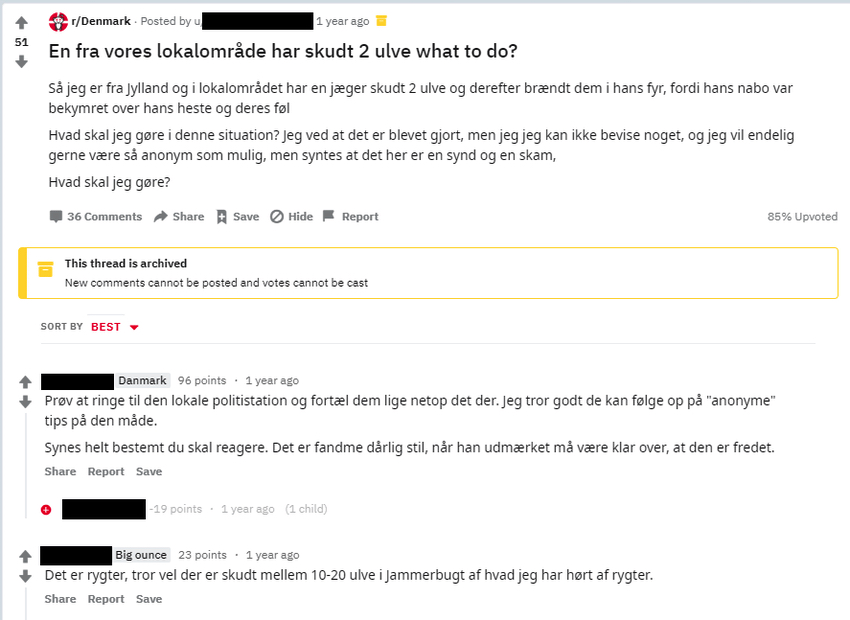
\includegraphics[width=\textwidth]{reddit}
\caption{Submission with comments \cite{reddit}}
\label{fig:reddit}
\end{figure}

The purpose of this chapter's analysis is to apply this existing literature and understanding of Russian methods of computational propaganda to the Reddit data (described in the introduction) with a focus on the Ukrainian crisis.
Reddit's content consists of submissions posted by users within subreddits (topical groups/communities); each submission may have replies (associated children comments), and each comment may have its own replies.
They form what is commonly called a ``thread'', or in formal terms, a ``tree'' because of its branches.
Figure \ref{fig:reddit} is an example submission with comments.

\begin{figure}[!ht]
\centering
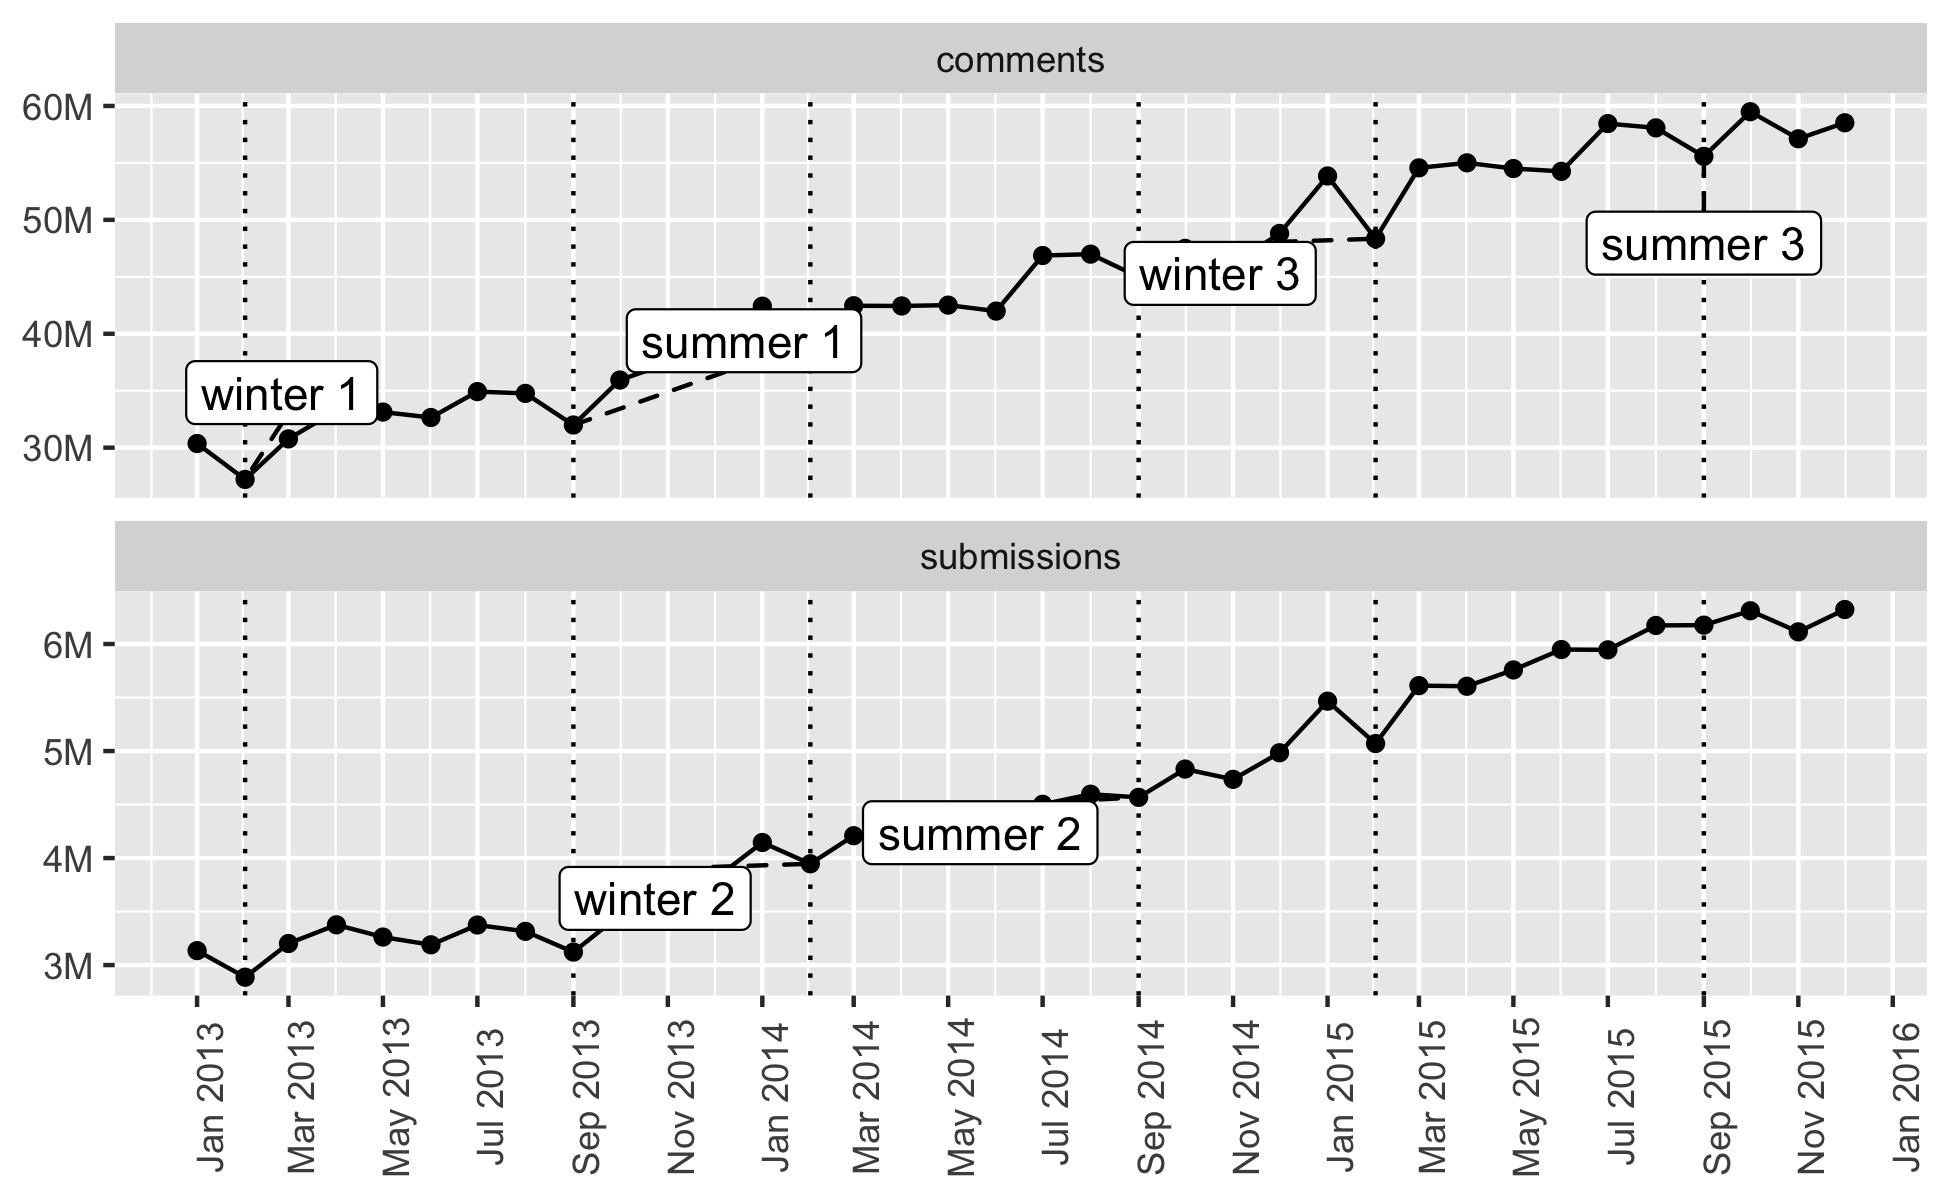
\includegraphics[width=\textwidth]{rus/count}
\caption{Comments and submissions}
\label{fig:count}
\end{figure}

The base dataset contains all 1,764,821,061 items or 163,041,230 submissions and 1,601,\\779,831 comments by 18,236,653 users across 460,025 subreddits on Reddit from January 2013 to December 2015.
These are freely available via Reddit's API, instead of downloading them ourselves, we use PushShift's archive which provides the very large dataset in an optimal compression format and has been used by other academic research \cite{pushshift}.
Figure \ref{fig:count} displays comments and submissions by month.

Though the most important events of the crisis start in late 2013 and end in  early 2015, the wider date range is selected to provide a control and context to capture change over time.
The total number of submissions and comments increases linearly each month, reflecting Reddit's growing popularity; in January 2013 there were 3,134,862 submissions and 30,365,867 comments, in December 2015 there were 6,322,479 submissions and 58,523,312 comments, increases of 101.68\% and 92.73\%.
The number of submissions and comments are directly correlated; over the three year period, the ratio of submissions to comments is never less than 9.42\% or greater than 11.11\%.

The most obvious pattern is a regular dip in activity at the end of each summer (September) and in winter (February).
Reddit's demographics skew younger such that this is probably connected to students returning to school after breaks.
This ``Eternal September'' has been recognized for decades.
Prior to the creation and adoption of the web, the Internet was used and populated by a much narrower range of people, usually professionals and experts at universities or self-selected early adopters and enthusiasts.
Usenet was a standard protocol which allowed users to send and receive messages in a format similar to Reddit; because new university students unfamiliar with norms gained access every year, September came to be dreaded by regular Internet users.
When AOL started offering consumer Usenet access in 1994, the previous September was said to have never ended \cite[p. 401]{isaacson2014}.

Next, the text component of each item (title and selftext for submissions, body for comments), is processed using the Python library spaCy. \footnote{The items, already divided into submissions and comments and split by month are downloaded from PushShift, decompressed into JSON, and saved into a format (Parquet) more appropriate for data work, split up by day.
The data include fields that are unnecessary for this research; for submissions only the id, created\_utc, edited, retrieved\_on, author, subreddit, url, title, and selftext fields are kept, for comments the id, created\_utc, edited, retrieved\_on, author, subreddit, link\_id, parent\_id, and body fields are kept.}
This natural language processing (NLP) toolkit uses modern techniques to correctly split (tokenize and parse) text in various languages into words, sentences, and other linguistic parts.
It also importantly converts words into vectors (lists, arrays, sequences) of numbers that are useful for computation and analysis, the basis of machine learning.

\begin{figure}[!ht]
\centering
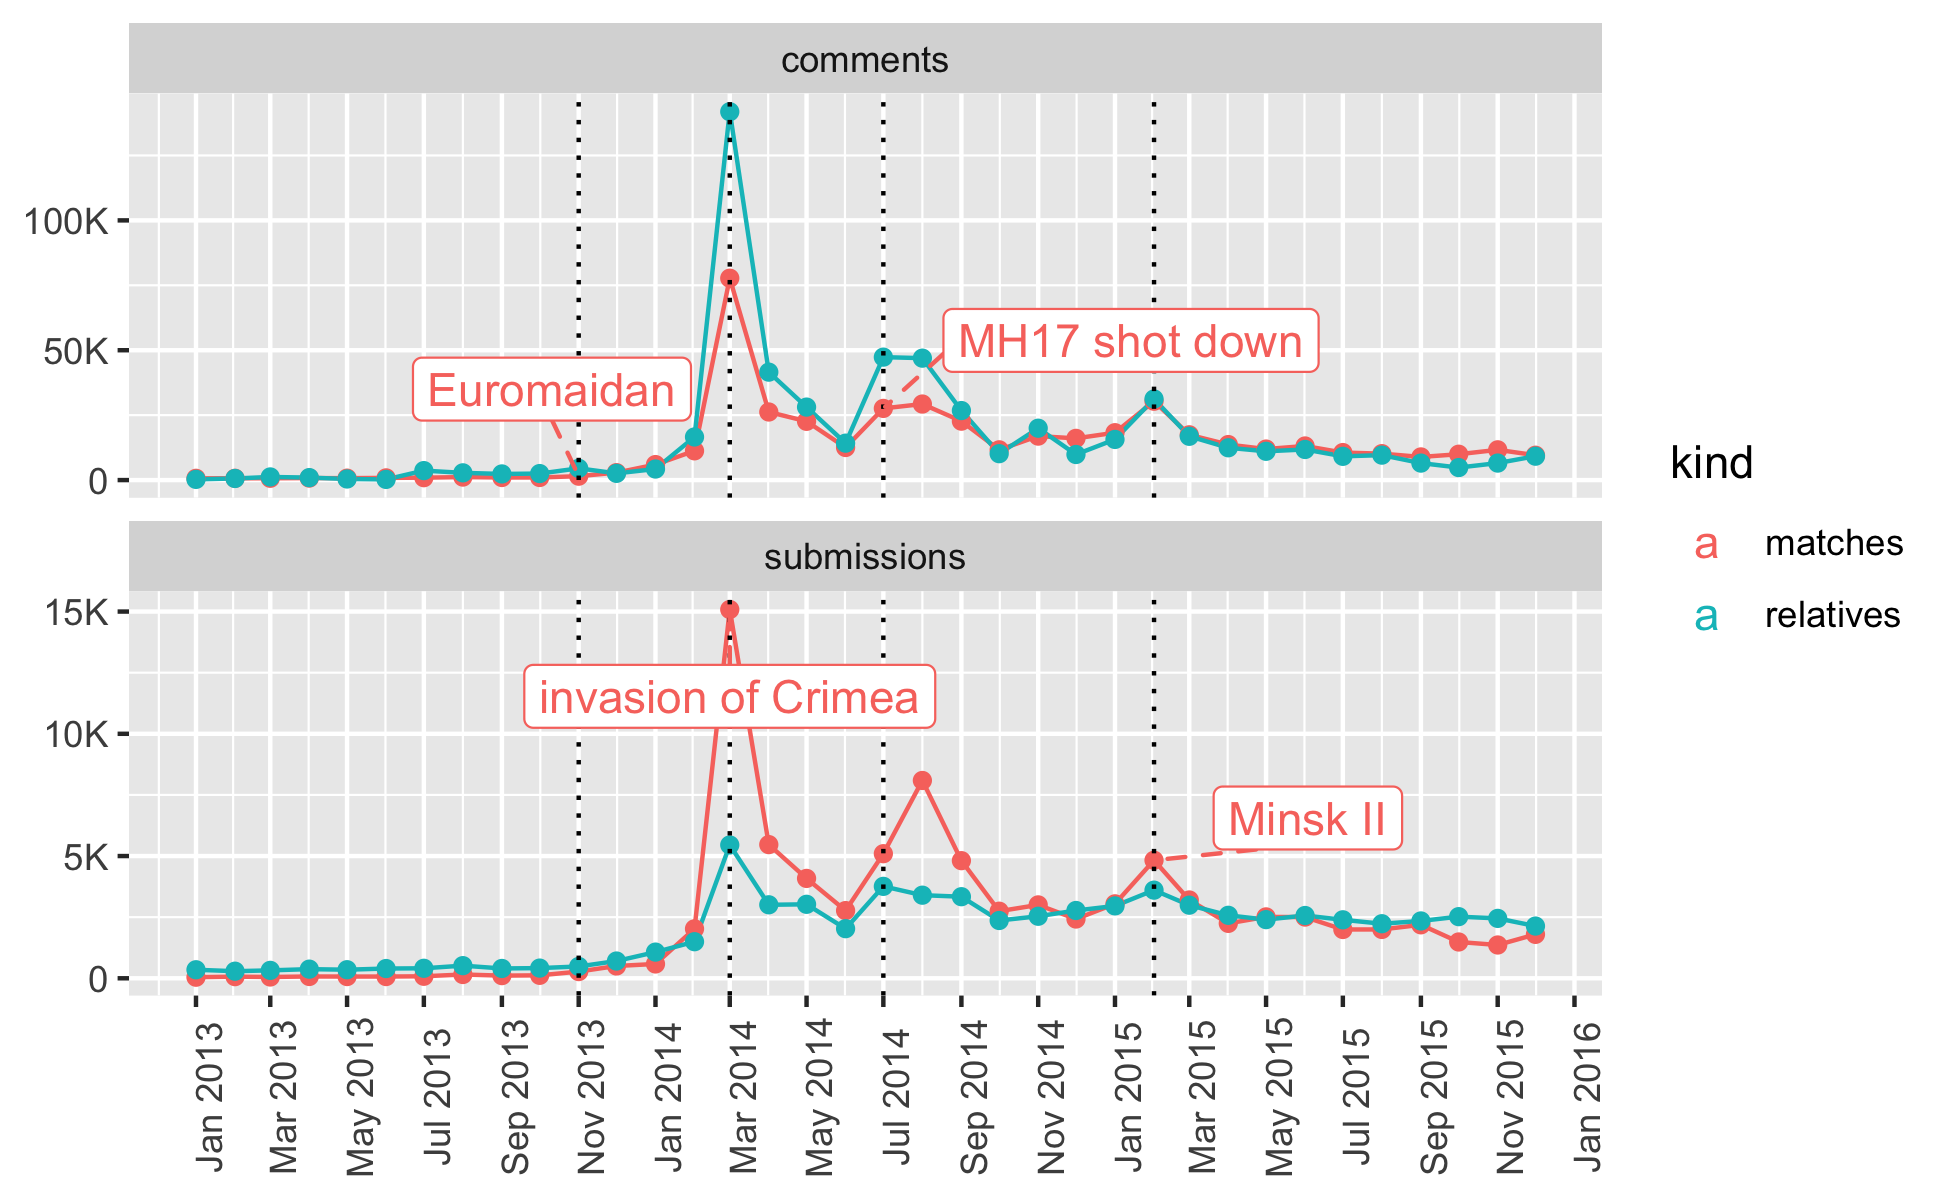
\includegraphics[width=\textwidth]{rus/things1}
\caption{Matches and relatives}
\label{fig:matches}
\end{figure}

The majority of items are irrelevant to the topic so the text of each item is filtered through a set of keywords and terms (case-insensitive).
The item is considered a ``match'' if ``Euromaidan'' or ``Donbas(s)'' are present, or if various combinations of ``Crimea'', ``Crimean(s)'', ``Putin'', ``Russia'', ``Russian(s)'', ``Ukraine'', ``Ukrainian(s)'', and terms related to ``annexation'' and ``invasion'' are found. \footnote{We only match against case-insensitive terms, an improvement would be to match against stems (used later in the chapter).}
In addition to these ``matches'', items connected to them are marked as ``relatives''.
For submissions, this includes every comment in response to it, for comments, this includes the submission the comment is in response to as well as any comments (children) replying to the match and the replies to those replies, etc.
Figure \ref{fig:matches} displays matches and relatives by month.

Euromaidan is a very unique term specific to the conflict and the Donbass region not commonly mentioned in Western popular media outside of the conflict
The dyads ensure we match on content including both countries or relevant topics (Putin, invasion) within the context of Russia, Ukraine, and Crimea.
Despite explicitly matching on Euromaidan, there is not a substantial increase in activity during that time (November 2013); that month there are 274 matched, 484 related submissions and 1,489 matched, 6,023 related comments.
Only in February 2014, the start of the invasion of Crimea, does there begin to be more matched than related submissions; this suggests that until this time it was a background topic brought up while discussing other primary topics.
Even then there are only 2,024 matched and 1,496 related submissions.
March 2014 follows with the peak of discussion: there are 15,084 matched, 5,453 related submissions, and 77,741 matched, 219,586 related comments, increases of 483.44\% for the submissions and 659.58\% for the comments.
The second peak of the comments is July 2014, the month of MH17's downing, with matched submissions rising the next month, even though ``MH17'' is not explicitly matched as a keyword.
February of 2015 is a third peak which is when the Minsk II ceasefire was signed, after that discussion returns to a similar level as in February 2014.
In total there are 86,969 matched, 70,447 related submissions and 459,053 matched, 1,033,697 related comments across the three years.
These patterns show that there are definite spikes and dips directly connected to the major events of the conflict and that our match terms are finding this relevant information.

\begin{table}[!ht]
\centering
\caption{Subreddits}
\begin{tabular}{lrrrrr}
\toprule
subreddit & \% & matches* & items & match \% & users \\
\midrule
worldnews             &   26.42 &   8643307 &    11747329 &    73.58 &   670840 \\
ukraine               &   10.39 &   3398449 &     4449535 &    76.38 &   226133 \\
UkrainianConflict     &    4.60 &   1504119 &     1765260 &    85.21 &   111672 \\
UkraineWarVideoReport &    3.46 &   1133154 &     1554034 &    72.92 &   125078 \\
CombatFootage         &    3.08 &   1007114 &     1543356 &    65.25 &   105349 \\
europe                &    2.22 &    725743 &     1857161 &    39.08 &    65027 \\
interestingasfuck     &    2.16 &    706541 &     4724053 &    14.96 &   218316 \\ß
news                  &    1.50 &    490912 &     5105814 &     9.61 &   102269 \\
politics              &    1.49 &    488251 &     6034055 &     8.09 &   111127 \\
AskARussian           &    1.46 &    476317 &      645065 &    73.84 &    25777 \\
conspiracy            &    1.40 &    458934 &     4302073 &    10.67 &    49986 \\
PublicFreakout        &    1.14 &    371466 &     5078293 &     7.31 &   106408 \\
neoliberal            &    1.09 &    355758 &     2846818 &    12.50 &    12885 \\
Damnthatsinteresting  &    1.06 &    348223 &     3066770 &    11.35 &   137484 \\
RussiaUkraineWar2022  &    0.82 &    269498 &      353670 &    76.20 &    35129 \\
ukpolitics            &    0.78 &    253829 &     1164034 &    21.81 &    10976 \\
NonCredibleDefense    &    0.69 &    226047 &      903671 &    25.01 &    21413 \\
nextfuckinglevel      &    0.65 &    211148 &     2937907 &     7.19 &    93475 \\
de                    &    0.62 &    201494 &     1500742 &    13.43 &    11344 \\
CryptoCurrency        &    0.55 &    181134 &     4980486 &     3.64 &    30981 \\
AskReddit             &    0.55 &    179205 &    39669986 &     0.45 &    56466 \\
ThatsInsane           &    0.51 &    168041 &     1069685 &    15.71 &    69375 \\
wallstreetbets        &    0.51 &    167041 &     7255226 &     2.30 &    46690 \\
Conservative          &    0.42 &    137499 &     1615715 &     8.51 &    19408 \\
CredibleDefense       &    0.34 &    112541 &      127050 &    88.58 &     6494 \\
russia                &    0.33 &    109417 &      171355 &    63.85 &    11906 \\
MapPorn               &    0.28 &     93019 &     1058404 &     8.79 &    32329 \\
canada                &    0.27 &     88474 &     1916732 &     4.62 &    16165 \\
CrazyFuckingVideos    &    0.26 &     85168 &     1691437 &     5.04 &    35943 \\
UkraineInvasionVideos &    0.26 &     84348 &      115132 &    73.26 &    13433 \\
summary (top 30)      &   69.32 &  22676191 &   121250848 &    32.64 &          \\
summary (all)         &  100.00 &  32713731 &  1456280549 &     0.49 &  2565090 \\
\bottomrule
\end{tabular}

\label{fig:subreddits}
\end{table}

These results are expected if the keyword filtering is correctly matching relevant data.
However, Reddit is divided into subreddits, which means that we can further remove large chunks of unrelated topics.
A common issue with social science datasets is sports can cause false positives; every four years in the World Cup or Olympics, countries ``battle'' countries and teams and fans ``invade'' the other team's stadium.
The World Cup semi-final between Brazil and Germany in 2014, games between Ukraine and Russia, or interactions between athletes from these countries have usually have limited connection to world politics.
Similarly, Reddit's demographics tend towards many discussions about videogames and e-sports, both of which are international interests.
Other topics are generally irrelevant to this research.
Therefore, out of the original set with at least 100 matches and relatives, 69 subreddits and their matches and relatives, including r/soccer, r/hockey, r/eurovision, r/languagelearning, and r/starcraft are excluded.
Table \ref{fig:subreddits} displays the 30 subreddits with the most matches and relatives.

There are total 1,560,766 matches and relatives by 193,560 users across 5,138 subreddits.
The r/worldnews subreddit accounts for 42.2\% of all matches and relatives, though only 3.48\% of all items in that subreddit are matches or relatives, slightly below the average mean of 4.8\% for the top 30.
The top 7 subreddits account for more than 73\% of all matches and relatives, and the top 30, 85.71\%. \footnote{This is a standard power law distribution, discussed later in this chapter.}
Only a few subreddits have to be targeted to monitor and direct these discussions and the Reddit homepage has and still does link to r/worldnews, directing users to it.
r/worldnews has the most unique users (85,829) in these discussions, only two other subreddits have more than 20,000 users, and r/russia has 4,578, r/ukraine 3,080, and r/conspiracy 3,875. 
It would take small numbers of users (real or not) to dominate these discussions, especially if we assume that the average user is not coordinating with others to push a narrative.
Finally, four subreddits have double-digit match rates, three: r/UkrainianConflict (37.56\%), r/russia (20.5\%), r/ukraine (46.16\%) have match rates over 20\%.

\subsection{Classification}

We need some way of detecting Russian propaganda and the users that post it.
There are many ways to categorize textual content and by extension the producers of that content.
These range from the relatively unsophisticated but time-tested manual coding of documents to an ever-expanding set of modern techniques.
The rise of machine learning has brought many supervised and unsupervised systems into play including naive Bayes classifiers, support vector machines, neural networks, and various natural language processing approaches.
Woolley and Guilbeault's analysis of the 2016 US presidential election via Twitter used BotOrNot, a software suite which takes into account a wide array of features to aid in bot detection \cite[p. 198]{woolley2018}.

These approaches all have strengths and weaknesses relative to a given dataset though many options would work fine for this particular study.
Our chosen method is based on a few specific goals.
While heavily influenced and modeled after Woolley and Guilbeault, this research not is particularly concerned whether a user is a ``bot'' or ``troll'', setting aside the muddled use of those terms.
The abundance of features these software suites take into account can be detrimental as they are highly specific, sensitive to the changing behavior of users constantly trying to avoid detection, and difficult to describe or justify to a non-technical audience.

Our intended audience is not just computer scientists or machine learning experts but political and other social scientists as well as a non-academic audience.
If the author fails to understand the complexities or nuances of neural networks or fails to impart that knowledge to the reader then confidence in the overall argument is lost.
Therefore, in classification and in each step of this research simple and pragmatic techniques are favored as they are easier to describe, defend, and debug.

For text and user classification we use an approach based on web addresses or URLs.
Google rose to prominence and profitability in the early 2000s thanks to their PageRank system which categorizes and ranks sites based on which sites in turn reference or link to them.
This was inspired by the custom of citations and references that powers academic research \cite[p. 462]{isaacson2014}.
To cite an author or work is to if not agree with them to at the very least acknowledge that said work has some kind of social currency; it is a form of provenance.

Web addresses themselves, not just the resources they reference, are often packed with information including the date, author, or title.
They always include a domain address, which is registred with in public information about the owner.
Given the assumption that individuals generally spread material that they agree with, by categorizing domains we can more broadly categorize content and the users that link to this content.
For example, \url{www.nytimes.com/2020/08/05/us/politics/state-department-russian-disinformation.html}.

\begin{table}[!ht]
\centering
\caption{Cites}
\begin{tabular}{lrrrrrr}
\toprule
{} & \% & cites & users &  cites / & \% prog & \% cons \\
domain &  &  &  & users & users & users \\
\midrule
reddit.com*           &   21.94 &   2722645 &   630963 &         4.32 &         13.41 &          9.79 \\
youtube.com*          &    9.62 &   1193237 &   251651 &         4.74 &         16.49 &         17.00 \\
imgur.com             &    6.01 &    746031 &   200126 &         3.73 &         10.76 &          9.57 \\
wikipedia.org         &    3.70 &    459470 &   126526 &         3.63 &         19.83 &         11.21 \\
twitter.com*          &    3.45 &    428391 &    81020 &         5.29 &         23.65 &         22.73 \\
washingtonpost.com    &    2.03 &    252175 &    68845 &         3.66 &         40.00 &         19.00 \\
nytimes.com*          &    1.37 &    170305 &    54124 &         3.15 &         32.52 &         16.96 \\
cnn.com               &    1.13 &    139847 &    47536 &         2.94 &         36.94 &         22.44 \\
archive.org*          &    1.06 &    131008 &    20095 &         6.52 &         29.30 &         37.80 \\
google.com*           &    1.05 &    130314 &    48537 &         2.68 &         16.23 &          9.06 \\
politico.com          &    0.97 &    120307 &    37074 &         3.25 &         45.09 &         26.10 \\
thehill.com           &    0.90 &    111112 &    30702 &         3.62 &         43.44 &         28.39 \\
theguardian.com       &    0.84 &    103685 &    39020 &         2.66 &         41.09 &         17.61 \\
huffingtonpost.com*   &    0.72 &     89205 &    32861 &         2.71 &         44.03 &         18.67 \\
sli.mg                &    0.72 &     88865 &    15886 &         5.59 &         10.85 &         22.45 \\
independent.co.uk     &    0.62 &     77328 &    22716 &         3.40 &         44.67 &         13.21 \\
reuters.com           &    0.56 &     69324 &    23100 &         3.00 &         36.07 &         23.85 \\
wikileaks.org         &    0.52 &     64918 &    12213 &         5.32 &         19.71 &         23.63 \\
breitbart.com         &    0.50 &     62530 &    17220 &         3.63 &         25.17 &         52.35 \\
politifact.com        &    0.49 &     60982 &    26742 &         2.28 &         32.46 &         13.41 \\
foxnews.com           &    0.46 &     57092 &    23051 &         2.48 &         24.60 &         35.29 \\
bbc.com*              &    0.43 &     53800 &    24014 &         2.24 &         22.17 &         17.11 \\
businessinsider.com   &    0.41 &     51133 &    24106 &         2.12 &         34.92 &         21.58 \\
fivethirtyeight.com   &    0.38 &     47223 &    18570 &         2.54 &         39.89 &         11.51 \\
facebook.com*         &    0.37 &     46391 &    18790 &         2.47 &         18.70 &         10.88 \\
nbcnews.com           &    0.37 &     46260 &    19792 &         2.34 &         42.94 &         20.70 \\
realclearpolitics.com &    0.34 &     42197 &    15416 &         2.74 &         34.86 &         20.09 \\
theatlantic.com       &    0.34 &     41577 &    19370 &         2.15 &         44.51 &         17.66 \\
go.com                &    0.33 &     41301 &    17435 &         2.37 &         44.54 &         17.30 \\
npr.org               &    0.31 &     38915 &    18260 &         2.13 &         43.26 &         13.57 \\
summary (top 30)      &   61.96 &   7687568 &          &         3.32 &         31.07 &         20.03 \\
summary (all)         &  100.00 &  11761790 &  1174637 &         1.97 &         45.13 &         41.51 \\
\bottomrule
\end{tabular}

\label{tab:doms}
\end{table}

This url contains a date, title, and topic (US politics), and is hosted on the New York Times (nytimes.com) domain.
We obtain all the domains in the dataset by extracting the url in each submission as well as those found in the body text of submissions and comments, using the already processed spaCy data.
Domains are then extracted from addresses, careful to take into account the variety of international suffixes including .co.uk. \footnote{Technically, the ``public suffix'' of the domain is captured using the publicsuffix2 Python library.}

The 30 most cited-domains are summarized in Table \ref{tab:doms}.
Domains from the previously excluded subreddits are not included, and we further filter the dataset by removing 8 users that are apparent bots, including u/AutoModerator and u/autotldr (an article summarizer), common across subreddits, and u/ModeratorLog and u/PoliticBot, which mirror other subreddits.
We also merge several related domains and ``link shorteners'' together; reddit.com and redd.it are different names for the same thing.

The distribution is top-heavy with 313,409 of 426,426 (68.61\%) citations distributed among these 30 domains submitted by 84,735 of 149,365 (56.73\%) users.
Wikipedia is the most cited, with 92,254 or 20.14\% of all cites despite being editable by anyone, prone to opaque conflicts between editors, and having been the target of multiple attempts by individuals, organizations, and state entities to whitewash reputations \cite{wiki:criticism}.
This tracks with the expectation of ``facts'' and evidence in the Russian blogosphere, a reaction to unreliable state media \cite[p. 25]{woolley2018}.
Wider Soviet and Russian disinformation has emphasized evidence, but it is not obvious whether this use of Wikipedia is a Redditism or widely-used elsewhere.

Reddit is another 18.40\% of cites; between it, Wikipedia, imgur.com, YouTube, and Twitter are more than 53.58\% of all links.
Facebook only has 1,509 cites, reflecting its parallel ``walled garden'' environment of personal connections.
The news sources themselves are distributed evenly across various regions with media in the UK (theguardian.com, bbc.com, telegraph.co.uk, dailymail.co.uk, independent.co.uk) and US (nytimes.com, washingtonpost.com, cnn.com, bloomberg.com, wsj.com) well-represented.
Ukrainian \\ (kyivpost.com) and independent Russian outlets are present (themoscowtimes.com) as well as aljazeera.com and globalresearch.ca.
Perhaps most notable are the multiple outlets owned, sponsored, or controlled by the Russian government: itar-tass.com, rt.com, and ria.ru.
Similarly, rferl.org, Radio Free Europe/Radio Liberty, is funded by the US government.
These Russian state domains are the basis of our categorization scheme.

We begin with a ``core'' list of 14 Russian government-owned or controlled domains including the official Kremlin site (kremlin.ru), Ministry of Defense site (mid.ru), and major domestic media providers (russia.tv, 1tv.ru, voiceofrussia.com).
To these are added domains controlled by the Iranian and Chinese governments: Press TV, Fars News, Xinhuanet, and China Daily.
These domains are all selected based on their presence within the dataset.
Our core assumption is that state media is unlikely to publish anything but state propaganda, or at the very least will not publish content contrary to the interests of the state.
If a user cites these sources often they are spreading, willingly or not, propaganda.

While all have government ties, they have different origins.
Rossiyskaya Gazeta (rg.ru) came into being in 1990 just before the fall of the USSR \cite{strovsky2021}.
Russia-24 (vesti.ru) and RT were founded during the Putin era \cite[p. 305]{yablokov2015}.
ITAR-TASS and RIA Novosti are much older, the former began in 1904 under the tsarist regime and continued into the Soviet era through today, and the latter was established in 1941 \cite{watanabe2017, simons2016}.
They are supplemented by a number of publications that while not officially government-owned have close ties and loyalties to the Kremlin, often through the convoluted system of oligarchs.
Izvestia (iz.ru) was founded in 1917 during the revolution and is today owned by Yuriy Kovalchuk's National Media Group; Kovalchuk is known as ``Putin's banker'' \cite{voltmer2000}.

These unofficially Kremlin-aligned sites are contained in a separate ``extended'' list with publications which have been appropriated; lenta.ru saw mass firings and resignations by the editorial staff in early 2014 in a shift towards propaganda \cite[p. 45]{lazitski2020}.
There are also a number of sites with hidden ties that are repeaters of the state line including Global Research (globalresearch.ca) and New Eastern Outlook (journal-neo.org); according to the US State Department, NEO presents itself as an academic journal \cite{nyt:globalresearch, statedept}.

We count domains with extremist anti-Semitic and conspiracy theorist views among the extended grouping.
Russia, like many other countries, has a troubled history of Jewish relations. 
When the surrounding countries divided up the Poland-Lithuanian Commonwealth at the end of the 18th century, the large population of Jews ended up Russian subjects (not citizens, not Russians), restricted to the Pale of Settlement in the west; in the late 19th and early 20th century there were numerous pogroms (mass violence) against these Jewish communities, this led to mass emigration to the United States and other countries.
In the early 1950s, at the height of his power, Stalin's prejudices and paranoias ended with him giving support to the arrest and torture of dozens of doctors in the medical community in a supposed Jewish ``Doctors' plot''; the media blitz of the Russian state media and the prosecution of the non-existent conspiracy stopped with his death in March 1953 \cite[ch. 56]{montefiore2007}.
Putin has used similar rhetoric, suggesting Jews (or Ukrainians or Tartars with Russian citizenship) were responsible for meddling in the 2016 presidential election in the US \cite{putin2018}.
Violence and rhetoric against Jews has increased in the US in recent years with the infamous ``tiki torch'' parade in Charlottesville in 2017, attacks in Pittsburgh in 2018, Poway, California and Jersey City in 2019, and numerous smaller incidents like the taking of hostages at a synagogue in Colleyville, Texas in 2022. 
The Unz Review (unz.com) and Russia Insider (russian-insider.org) engage in Holocaust denial and anti-Semitic stances along with generally favorable coverage of Russia \cite{bevensee2018}.

This anti-Semitic content often overlaps with conspiracy theories and can be found on the political extremes.
One dominant notion is that of false flags where (usually) the United States government is said to engage in covert actions against its own citizenry to allow for increased control or military engagement, the primary example being the 9/11 truther movement.
Starting with the claims of ``crisis actors'' in the Sandy Hook school shootings in 2012, it is perhaps difficult to find events of mass violence not claimed to be fake.
Conspiracy theories are well-represented in Alex Jones-owned domains: InfoWars (infowars.com) and PrisonPlanet (prisonplanet.com).
Jones has made numerous claims of false flags and in 2022 was ordered to pay \$45.2 million in punitive damages to the parents of a victim of Sandy Hook \cite{jones2022}.

The basis and probable cause of many of these claims is due to US military action.
Veterans Today (veteranstoday.com) explicitly targets former US service members with a pro-Russian message and was partners with NEO \cite[p. 24]{statedept}..
We include a number of domains in the extended list for content which while critical and skeptical of neoliberal US foreign policy, fails to apply that same skepticism to Russian intentions, in some cases parroting Kremlin-associated material.
On the right of the political spectrum are sites favorable to former Republican presidential candidate and long-time libertarian Ron Paul: Ron Paul Institute (ronpaulinstitute.org) and The Daily Bell (thedailybell.com).
The left is represented by OpEdNews (opednews.com) and Antiwar.com.
This kind of selectivity critical reporting is reminiscent of Western liberals like Walter Duranty, former Moscow Bureau Chief of the New York Times.
Despite winning a Pulitzer for favorable reporting on the USSR in the early 1930s, at the same time he repeatedly denied the famine in Ukraine known as the Holodomor \cite[p. 445]{dutton2005}.

\begin{table}[!ht]
\centering
\caption{Rus domains}
\begin{tabular}{rlrrrrr}
\toprule
rank & domain &       \% &  cites &  users &  cites/users &  \% rus users \\
\midrule
9                &                         rt.com &   27.07 &   5425 &   2070 &         2.62 &        43.91 \\
16               &                 itar-tass.com* &   10.21 &   2046 &    624 &         3.28 &        63.83 \\
25               &                         ria.ru &    6.35 &   1272 &    513 &         2.48 &        51.65 \\
27               &              globalresearch.ca &    6.18 &   1238 &    625 &         1.98 &        37.72 \\
30               &                  zerohedge.com &    5.74 &   1150 &    458 &         2.51 &        51.30 \\
34               &                sputniknews.com &    5.40 &   1082 &    382 &         2.83 &        61.37 \\
52               &            ian56.blogspot.com* &    3.30 &    661 &      6 &       110.17 &        98.49 \\
57               &             russia-insider.com &    3.04 &    610 &    141 &         4.33 &        77.21 \\
66               &              voiceofrussia.com &    2.61 &    523 &    242 &         2.16 &        45.89 \\
67               &                       lenta.ru &    2.60 &    521 &    194 &         2.69 &        55.28 \\
92               &                      pravda.ru &    1.88 &    377 &    181 &         2.08 &        53.32 \\
102              &                     kremlin.ru &    1.66 &    332 &    162 &         2.05 &        48.49 \\
103              &                    antiwar.com &    1.65 &    331 &     92 &         3.60 &        76.44 \\
108              &                       rbth.com &    1.55 &    311 &    132 &         2.36 &        58.84 \\
128              &            washingtonsblog.com &    1.26 &    253 &    110 &         2.30 &        59.68 \\
145              &                   infowars.com &    1.07 &    215 &     86 &         2.50 &        54.88 \\
153              &  informationclearinghouse.info &    1.04 &    208 &     98 &         2.12 &        61.06 \\
156              &                      gazeta.ru &    1.00 &    201 &    132 &         1.52 &        36.32 \\
165              &                     presstv.ir &    0.93 &    187 &    123 &         1.52 &        34.76 \\
169              &                     ukraina.ru &    0.91 &    183 &     16 &        11.44 &        90.71 \\
181              &                       sott.net &    0.85 &    170 &     75 &         2.27 &        65.29 \\
193              &                    rusvesna.su &    0.79 &    159 &     83 &         1.92 &        47.17 \\
196              &                    lifenews.ru &    0.78 &    156 &     93 &         1.68 &        46.15 \\
203              &                voltairenet.org &    0.73 &    146 &     71 &         2.06 &        53.42 \\
207              &                  xinhuanet.com &    0.72 &    144 &     91 &         1.58 &        45.83 \\
214              &                       vesti.ru &    0.68 &    137 &     84 &         1.63 &        35.77 \\
216              &                         mid.ru &    0.68 &    136 &     64 &         2.12 &        57.35 \\
227              &           paulcraigroberts.org &    0.64 &    128 &     61 &         2.10 &        53.91 \\
235              &           ronpaulinstitute.org &    0.61 &    122 &     55 &         2.22 &        43.44 \\
280              &              beforeitsnews.com &    0.48 &     96 &     57 &         1.68 &        23.96 \\
& summary (top 30) &   92.40 &  18520 &   7121 &         6.19 &        54.45 \\
& summary (all)    &  100.00 &  20043 &   7853 &         4.30 &        58.11 \\
\bottomrule
\end{tabular}

\label{tab:rus_doms}
\end{table}

Of course, any categorization based on site content alone is subjective.
This arbitrariness is one of the criticisms leveled at other compilation attempts of pro-Russian sources like PropOrNot \cite{chen2016}.
Importantly, all domains included in the extended list have a higher percentage of citations from ``rus users'' that post these pro-Russian domains, core and extended.
For example, of all citations of nytimes.com, 21.05\% are from users that have cited these selected domains at least 10 times over the three-year period in the original dataset.
In comparison, russia-insider.com is at 77.21\% and ronpaulinstitute.org is at 43.44\%; of the 30 most-cited domains in Table \ref{tab:doms} (average 26.59\%), 18 have rates below 25\%, but of the 30 most-cited domains from the core and extended set (average 54.45\%), only 4 are below 40\%.
We assume that individuals will cite material which they not only agree with but which generally agrees with other material they have posted.
Since users have the ability to delete accounts on Reddit, in order to not overcount cites by rus users, we remove the specially marked ``[deleted]'' user.
Table \ref{tab:rus_doms} displays summary stats for the rus domains.

This list is top-heavy with 92.40\% of all citations of pro-Russian domains; the 3 most-cited (itar-tass.com, rt.com, ria.ru) are from the core set and are a combined 43.63\% of cites, they are ranked 9th, 16th, and 25th of all links posted about this topic.
The first domain not from the core set is globalresearch.ca (ranked 27th overall) with content from Jones, Unz, and numerous other conspiracy-focused entities.
37.72\% of all users that post it are ``rus'', compared to 43.91\%, 63.83\%, and 51.65\% of the first 3 and the overall mean of 58.11\%.
It also is the only of the first 17 rus domains with fewer than 2 cites per user; this suggests organic activity.

The sum activity is small; domains from the rus core and extended lists total 
20,043 cites by 7,853 users, 4.70\% of 426,426 total cites across all domains.
Of the rus set, rt.com is cited by the most users (2,070), ian56.blogspot.com by 6; ``Ian56'' is a known Russian troll across social networks \cite[p. 278]{heffer2020}.
Of 331 cites by 92 users of antiwar.com, 76.44\% were by rus users.
These numbers suggest that a very limited set of users are responsible for most of the ideological content on this topic, pro-Russians posting antiwar content is framing that is only obvious when those cites are aggregated.

Finally, the presence of Paul Craig Roberts' site is worth noting.
Assistant Treasury Secretary during the Reagan administration, he has since become a writer for unz.com, has been featured on RT as a guest, is a 9/11 ``Truther'', argued for Holocaust denialism and other conspiracy theories, and was accused of ``Putin worship'' \cite[p. 2388]{marmura2014}.
He is an example of a small but prominent group of individuals and institutions which favor and legitimatize each other.

\begin{table}[!ht]
\small
\centering
\caption{Wiki articles}
\begin{tabular}{lrrrrr}
\toprule
{} &       \% &  cites &  users &  cites/ & \% rus \\
wikipedia.com/wiki/                                               &         &        &        & users & users             \\
\midrule
Ukraine                                            &   10.92 &   1056 &     90 &        11.73 &         1.80 \\
Budapest\_Memorandum\_On\_Security\_Assurances         &    5.97 &    577 &    425 &         1.36 &         6.59 \\
Holodomor                                          &    5.35 &    517 &    312 &         1.66 &         4.64 \\
Crimea                                             &    4.97 &    481 &    179 &         2.69 &         5.41 \\
Euromaidan                                         &    4.11 &    397 &    152 &         2.61 &        14.36 \\
2014\_Crimean\_Crisis                                &    3.36 &    325 &     48 &         6.77 &        14.77 \\
Crimean\_Status\_Referendum,\_2014                    &    3.29 &    318 &    176 &         1.81 &        15.09 \\
Covert\_United\_States\_Foreign\_Regime\_Change\_Actions &    3.16 &    306 &    173 &         1.77 &        30.72 \\
Whataboutism                                       &    2.69 &    260 &    168 &         1.55 &        11.15 \\
Nuclear\_Weapons\_And\_Ukraine                        &    2.42 &    234 &    115 &         2.03 &         3.42 \\
Iran\_Air\_Flight\_655                                &    2.13 &    206 &    161 &         1.28 &         4.37 \\
2014\_Ukrainian\_Revolution                          &    2.05 &    198 &     73 &         2.71 &         9.09 \\
Russo-Georgian\_War                                 &    1.87 &    181 &    136 &         1.33 &        14.92 \\
Viktor\_Yanukovych                                  &    1.86 &    180 &     61 &         2.95 &         2.78 \\
Annexation\_Of\_Crimea\_By\_The\_Russian\_Federation     &    1.86 &    180 &     89 &         2.02 &         3.89 \\
Ukrainian\_Insurgent\_Army                           &    1.59 &    154 &     86 &         1.79 &         9.74 \\
Siberia\_Airlines\_Flight\_1812                       &    1.59 &    154 &    125 &         1.23 &        10.39 \\
Crimean\_Referendum,\_1994                           &    1.56 &    151 &     81 &         1.86 &        26.49 \\
Stepan\_Bandera                                     &    1.54 &    149 &     97 &         1.54 &        19.46 \\
Right\_Sector                                       &    1.50 &    145 &     87 &         1.67 &         8.28 \\
Svoboda\_(Political\_Party)                          &    1.47 &    142 &     93 &         1.53 &         5.63 \\
Deportation\_Of\_The\_Crimean\_Tatars                  &    1.44 &    139 &    109 &         1.28 &         9.35 \\
Crimean\_Tatars                                     &    1.44 &    139 &     56 &         2.48 &         2.88 \\
Massacres\_Of\_Poles\_In\_Volhynia\_And\_Eastern\_Galicia &    1.40 &    135 &     81 &         1.67 &        30.37 \\
2014\_Pro-Russian\_Unrest\_In\_Ukraine                 &    1.39 &    134 &     58 &         2.31 &         8.96 \\
Crimean\_War                                        &    1.39 &    134 &     76 &         1.76 &         4.48 \\
Igor\_Girkin                                        &    1.37 &    132 &     73 &         1.81 &        15.91 \\
Azov\_Battalion                                     &    1.30 &    126 &     85 &         1.48 &        20.63 \\
Tu\_Quoque                                          &    1.29 &    125 &     60 &         2.08 &         6.40 \\
Ukrainian\_Presidential\_Election,\_2010              &    1.23 &    119 &     68 &         1.75 &        13.45 \\
summary (top 30)                                   &   77.50 &   7494 &   3593 &         2.35 &        11.18 \\
summary (all)                                      &  100.00 &   9670 &   5126 &         1.93 &        11.34 \\
\bottomrule
\end{tabular}

\label{tab:wiki}
\end{table}

In the way these individuals and sources are telling points of reference, facts and events can serve the same purpose; we end this section with a review of commonly cited Wikipedia articles in Table \ref{tab:wiki}.
The sum activity is once again small, though Wikipedia was the most-cited domain, only 9,670 links by 5,126 users are extractable articles, of which the 30 most-cited account for 77.50\%.
Only 3 articles have more than 2.95 cites per user.
Pro-Russian users strongly favor certain topics and articles, those over the average of 11.34\% of rus users track Russian talking points.

The Budapest Memorandum (6.59\% rus users) was a multilateral agreement signed in 1994 which promised to respect the territorial integrity of Ukraine; multiple countries accused Russia of breaking this agreement with the invasion of Crimea.
Nuclear weapons and Ukraine may have a low rus cite percentage (3.42\%) because Ukraine surrendering their nuclear weapons to Russia was part of the deal.
The Holodomor (4.64\%) was the mass starvation of Ukrainians as a policy of the USSR in the early 1930s; the Crimean Tatars were (2.88\%) displaced over the centuries, faced Nazi atrocities, mass deportation during World War II due to alleged Nazi collaboration (9.35\%), then were banned from return until 1989.
The Tatars were an estimated 98\% of the population when Crimea was originally annexed in 1783, by 2004 that number was 12\%.

Covert Foreign regime change actions of the US has the highest rus percentage (30.72\%); the Russo-Georgian War (14.92\%) is oft-cited as an example of Western expansion into Russia's traditional sphere of influence.
Other apparent examples of whataboutism are attempts to tie the downing of MH17 to past downings of civilian planes.
Flight 655 was a downing by the USS Vincennes in 1988, Flight 1812 was a downing by Ukraine in 2001.
Igor Girkin (15.91\%) is a hard-line Russian nationalist, active in military actions throughout the conflict, former Supreme Commander of the self-proclaimed Russian ``Donetsk People's Republic'' accused of multiple atrocities including the downing of MH17.

One of the common talking points of Russian propaganda around the Ukrainian conflict is to paint the Ukrainian government as fascist and to associate it with Nazi actions in World War 2.
The Azov Battalion (20.63\% rus users) and Right Sector are far-right paramilitary groups operating in Ukraine against Russian interests.
Svoboda is an ultranationalist political party.
The volunteer battalion especially would become a feature of Russian propaganda, a justification for war in 2022 after it was reorganized and integrated into the Ukrainian National Guard in late 2014.
Stepan Bandera (19.46\%) was a fascist during World War 2 responsible for a number of atrocities, Putin has invoked him directly as a justification for Crimea's annexation: ``...saving them from the new Ukrainian leaders who are the ideological heirs of Bandera, Hitler's accomplice during World War II'' \cite[p. 204]{garcia2016}.
``Banderites'' and related terms are tells of Russian propaganda, he is not well-known in the US.
The Volhynia massacres (30.37\%) were carried out by the Ukrainian Insurgent Army, formed in October 1942 by Banderas' followers to fight Soviets and Nazis.

The multiple referenda are instructive.
Crimea has a majority Russian population as does much of southeastern Ukraine, in a state of insurgency since 2014.
Not surprisingly, referenda there tend to favor Russian interests, and the 2014 referendum in particular has been considered illegitimate by most countries due to Russian intervention.
The article for that year's referendum is cited by 16.09\% rus users, the 1994 version has the third-highest rus user percentage of 26.49\%.
These fit the confusing pattern of authoritarian regimes embracing democracy and popular will when convenient.

\begin{table}[!ht]
\centering
\caption{User groups}
\begin{tabular}{lrrrrrr}
\hline
& & & comment & comment & submission & submission \\
group & users & doms & matches & relatives & matches & relatives \\
\hline
neutral &  193647 &  346457 &           381264 &             776965 &               39312 &                 52842 \\
spreader &     262 &   80023 &            40618 &              52658 &               19011 &                  7143 \\
superspreader &      75 &   43239 &            13201 &              16223 &               13280 &                  3118 \\
totals &  193910 &  518141 &           459054 &            1033697 &               87008 &                 72688 \\
\hline
\end{tabular}

\label{tab:rus_groups}
\end{table}

Wikipedia articles are useful to provide context, but they are not included in either the core or extended list of Russian domains.
Using the combined list we are able to categorize users as shown in Table \ref{tab:rus_groups}.
Users that cite these domains at least 10 times over the three-year period of the dataset are considered ``spreaders'' of pro-Russian propaganda, with this limit used as a buffer to allow for unintentional activity.
Those that cite them 25 or more times are considered ``superspreaders''.
Too low of a cutoff will capture incidental posters or those that post a large and wide variety of material, too high of a cutoff removes the users we most want to capture, but these are arbitrary thresholds.
Without filtering subreddits, of the 193,910 users in the matched dataset, 193,647 (99.86\%) are neutral with fewer than 10 cites, 262 (0.14\%) are spreaders of pro-Russian content with at least 10 but less than 25 cites, and another 75 (0.04\%) are superspreaders with at least 25 cites. 
The totals include bots; the rest of the table shows pro-Russian users are a very small part of the dataset.

\subsection{Network Analysis}

With users categorized we can observe how they are distributed and how they interact using network analysis.
We want to know how the user network is shaped, whether pro-Russian users exist in their own isolated communities, or if they are ignored by others or receive many responses from a variety of people and therefore drive discussion.
Has Russian propaganda reached positions of influence within the core of the network?

Network analysis consists of statistical techniques that take into account features within networks (graphs) to determine their overall shape and layout. Graphs are composed of nodes (such as users) and their edges (connections). Graphs can be directed (displaying the flow of connections and information) or undirected (only showing that there is a connection).
Nodes have overall degree (the number of nodes which connect to them) and in the case of directed networks in-degree (incoming connections) and out-degree (outgoing connections) \cite[pp. 199-200]{woolley2018}.
There are many useful measures within graph theory but how useful those measures are and indeed the very basis of a graph is arbitrary and dependent upon the data and its interpretation.
It is up to the researcher to turn unstructured content into a truly representative model.
We use the NetworkX library, written in Python, to build and analyze our graphs.

\begin{figure}[!ht]
\centering
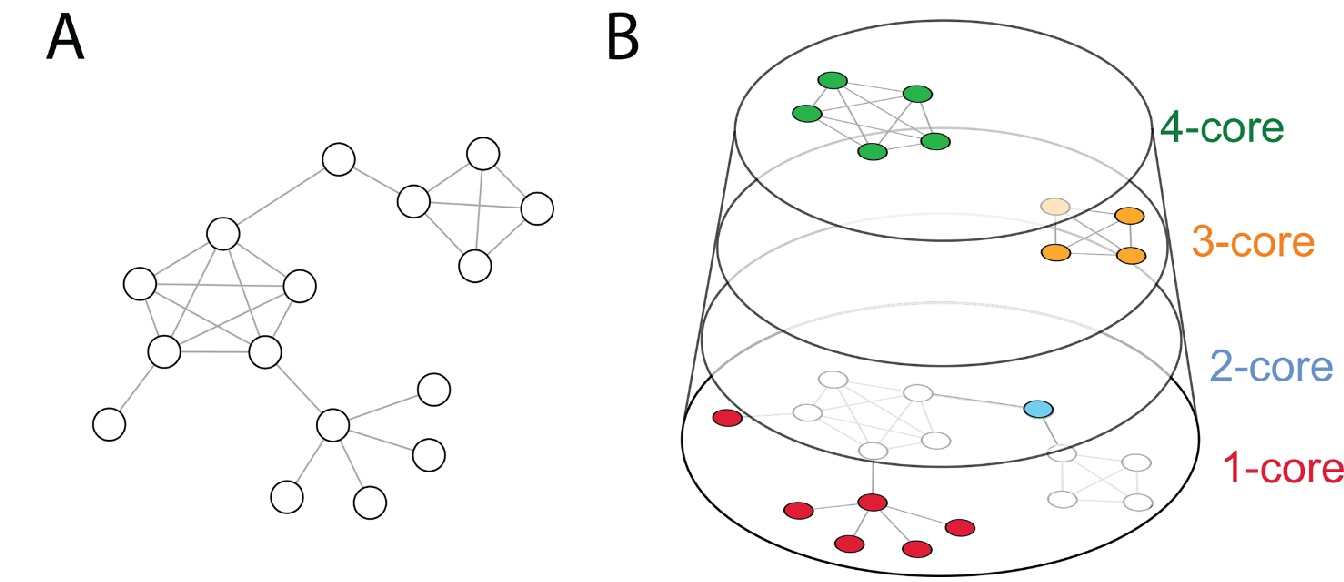
\includegraphics[width=\textwidth]{rus/kcore}
\caption{k-core \cite{barbera2015}}
\label{fig:kcore}
\end{figure}

Our first analysis consists of k-core decomposition.
This decomposition splits the largest-connected component of a network (subset of the network with the most connected nodes) into k-shells where each individual shell is composed of all nodes with the same or higher number of connections.
Specific cores contain multiple shells: the 10-core contains k-shells 1 through 10.
K-core decomposition is mostly dependent upon a node's degrees.
Nodes located in the highest shells have the most connections and are most able to disseminate information through the network and nodes in the lower shells are on the periphery \cite[p. 200]{woolley2018}.
Figure \ref{fig:kcore} illustrates the k-core for a random graph.

To reiterate, the structure of many graphs is arbitrary.
The same data can be represented in a graph that connects different nodes using different criteria, is directed or undirected, or has different weights measuring the strength of connections between nodes.
Woolley and Guilbeault base their k-core analysis on a network of Twitter users where connected users have both retweeted each other \cite[p. 202]{woolley2018}.
In order to capture the strictest measure of connection, our k-core analysis is run on an undirected network where nodes (users) have any edge (tie) only if they have posted in response (directly or to a child reply) to each other at least once.
We want to capture users that are interacting, not just those that post a lot of content (spam) but are ignored by the rest of the network.

\begin{figure}[!ht]
\centering
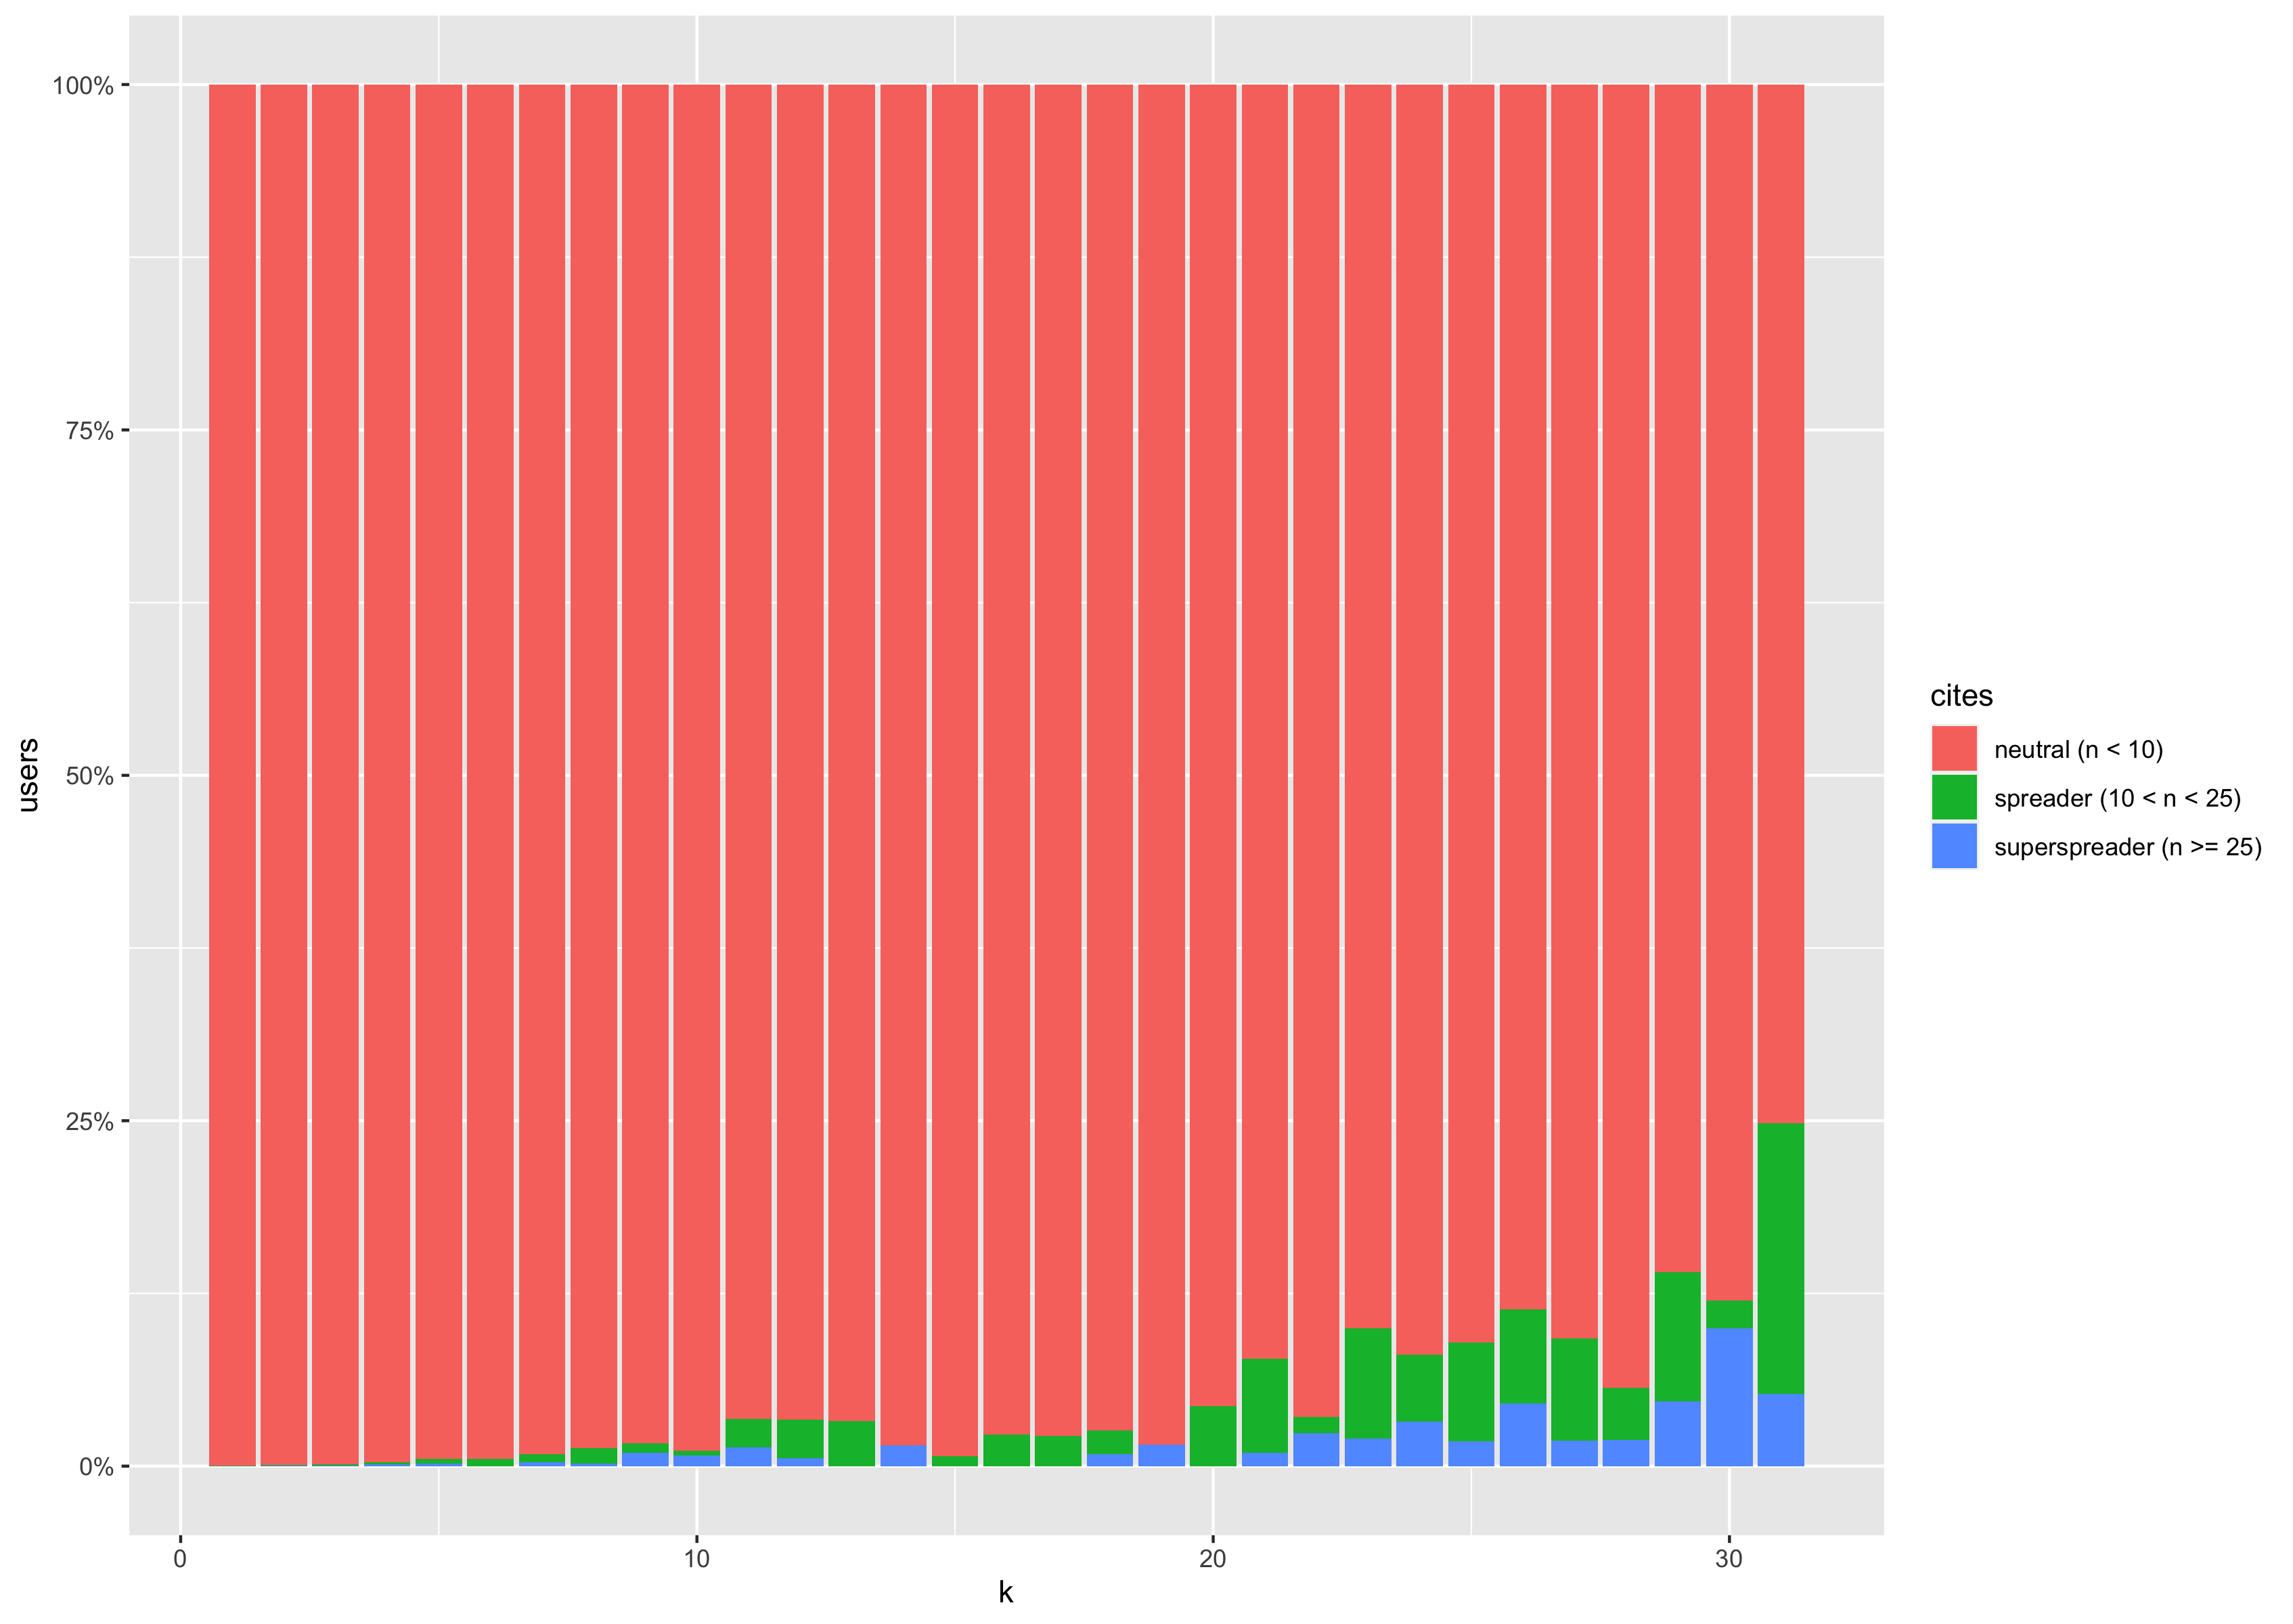
\includegraphics[width=\textwidth]{rus/kshells}
\caption{K-shells}
\label{fig:kshells}
\end{figure}

Figure \ref{fig:kshells} displays the k-core distribution.
The largest-connected component of the user network is composed of 59,009 users, 166 (0.28\%) are spreaders of Russian propaganda with at least 10 and less than 25 cites of domains in the combined Russian domain list, 66 (0.11\%) are superspreaders with at least 25 cites.
In total numbers (not depicted), neutral users have an extreme skew to the right with 53,808 (91.19\%) users located in the first 5 shells (on the periphery).
In contrast both the spreaders and superspreaders are more distributed in the higher shells; 168 (72.51\%) spreaders or superspreaders are found in shells 10 through 31, 132 (56.90\%) are found in shells 20 and higher, 76 (32.76\%) are found in the top shell, 26.66\% of all superusers.
Just as importantly, in the higher shells, rus users are a large percentage of all users, the top shell (31) is 24.87\% rus.
This indicates that Russian propaganda has reached positions of influence within the core of the network.

\begin{table}[!ht]
\footnotesize
\centering
\caption{Most ties in top k-shell}
\begin{tabular}{lrrllrl}
\toprule
 & ties & rus & top rus dom & top dom & cites & subreddit \\
user & & cites & & & & \\
\midrule
vigorous         &   856 &       1061 &      itar-tass.com &  itar-tass.com &    279 &          worldnews \\
holocauster-ride &   585 &         67 &              rt.com &  wikipedia.org &     91 &          worldnews \\
chewbacca81      &   574 &         18 &         rusvesna.su &  wikipedia.org &    145 &             russia \\
putupyourdukes   &   541 &          5 &   globalresearch.ca &  wikipedia.org &     50 &          worldnews \\
istinspring      &   483 &         34 &              rt.com &  wikipedia.org &    176 &             russia \\
Gibbit420        &   461 &         13 &              rt.com &  wikipedia.org &     75 &  UkrainianConflict \\
DisregardMyPants &   460 &         12 &              ria.ru &  wikipedia.org &     61 &  UkrainianConflict \\
spankaway        &   459 &          8 &              ria.ru &  wikipedia.org &     60 &  UkrainianConflict \\
4ringcircus      &   426 &          2 &              rt.com &  wikipedia.org &     13 &             russia \\
kornjacanasolji  &   415 &          6 &              mid.ru &  wikipedia.org &     43 &          worldnews \\
Glideer          &   408 &          9 &      newcoldwar.org &  wikipedia.org &     28 &  UkrainianConflict \\
Kuklachev        &   407 &          7 &              ria.ru &    youtube.com &     98 &  UkrainianConflict \\
kwonza           &   400 &          9 &               rg.ru &  wikipedia.org &     21 &          worldnews \\
ThePandaRider    &   378 &         10 &   globalresearch.ca &  wikipedia.org &     58 &  UkrainianConflict \\
WeAreBRICS       &   375 &         18 &              rt.com &  wikipedia.org &     35 &             russia \\
HighDagger       &   373 &         20 &         rusvesna.su &  wikipedia.org &    319 &          worldnews \\
JasonYamel       &   367 &          4 &            lenta.ru &  wikipedia.org &     69 &             europe \\
Infidius         &   356 &         14 &              rt.com &  wikipedia.org &     18 &          worldnews \\
turdovski        &   346 &         25 &  russia-insider.com &    youtube.com &    636 &             russia \\
kinmix           &   346 &          9 &              rt.com &  wikipedia.org &     57 &  UkrainianConflict \\
eugene7          &   345 &         13 &         lifenews.ru &    twitter.com &    104 &  UkrainianConflict \\
mkvgtired        &   340 &          6 &   globalresearch.ca &  wikipedia.org &     23 &             europe \\
9A4172           &   337 &          9 &              rt.com &    youtube.com &     21 &  UkrainianConflict \\
SpaceRaccoon     &   335 &         23 &      itar-tass.com &    youtube.com &    120 &             russia \\
orion4321        &   327 &          9 &  orientalreview.org &    youtube.com &    122 &  UkrainianConflict \\
Nilbop           &   326 &          6 &      itar-tass.com &  wikipedia.org &    116 &             europe \\
mrv3             &   323 &          8 &        infowars.com &  quickiwiki.com &     21 &          worldnews \\
LucifersCounsel  &   322 &         26 &              rt.com &  wikipedia.org &    182 &          worldnews \\
Vysotsky2        &   321 &         14 &              rt.com &    twitter.com &    112 &             russia \\
Rinnve           &   321 &         20 &           gazeta.ru &  wikipedia.org &     51 &          worldnews \\
\bottomrule
\end{tabular}

\label{tab:user_ties}
\end{table}

We further analyze the users of the top shell in Table \ref{tab:user_ties}.
The user with by far the most ties (856) with other users as well as citations of pro-Russian domains is the aptly-named u/vigorous.
This user is among 5 superspreaders in the top 30 with another 11 spreaders: rus users are 53.33\% of the 30 users with the most ties in the top shell.
15 prefer itar-tass.com, rt.com, or ria.ru out of our tagged Russian domains, but only u/vigorous cites them more than any other domain (279 times), and is one of 10 users whom post most often in the r/worldnews subreddit.
Unaware, non-partisan users are more likely to run into this biased content there than the other 3 subreddits favored by these top users.

Worth noting is the prevalence of Wikipedia.
21 of 30 users (70\%) cite it more than any other domain with 16 (53.33\%) of those citing it more than 50 times.
This presents a unique environment for the average user with no strong ties to or knowledge of the topic.
On the average thread some portion of it will contain users discussing the Ukrainian crisis with links to the at least nominally objective and accurate (and trusted) Wikipedia alongside disguised propaganda such as Oriental Review.
Oriental Review and users posting disinformation can either use complete falsehood or more-effectively (as the Wikipedia citations suggest) frame an event or fact in a way favorable to their position.

What dynamics are diving these user patterns?
Why is this relatively small set of users that post often salacious material from organizations out of the mainstream producing so much engagement?
It is probable that on a relatively niche (or non-salient) topic that this material does convince some of those that were uninformed.
However, it may be just as effective to divert the attention and resources of users with opposite positions by goading them on with controversy; by having the discussion there is the appearance of a contested concept, perhaps the main impression of the uninterested user.
King, Pan, and Roberts' research of the Chinese government's ``50c'' army shows ``strategic distraction'' itself has value \cite{king2017}.
Besides the noise it adds to the discussion, it is possible that trolling operations that are targeted internationally have a side-effect or goal of convincing domestic populations, too.
The r/russia subreddit, for example, provides an outlet to the West that may attract Russians at home and abroad; by virtue of being a foreign source it appears open but could be heavily manipulated.

\begin{table}[!ht]

\centering
\caption{Users by betweenness centrality}
\begin{tabular}{lrrrrll}
\toprule
 & bet & in & out & rus & dom & subreddit \\
user & cent z & deg z & deg z & cites & & \\
\midrule
holocauster-ride &       57.40 &     30.63 &      14.02 &         67 &   wikipedia.org &          worldnews \\
vigorous         &       52.42 &     26.16 &      45.72 &       1061 &   itar-tass.com &          worldnews \\
HighDagger       &       50.20 &     23.97 &       7.72 &         20 &   wikipedia.org &          worldnews \\
DisregardMyPants &       40.14 &     22.37 &       9.67 &         12 &   wikipedia.org &          worldnews \\
4ringcircus      &       34.59 &     21.42 &       7.49 &          2 &   wikipedia.org &             russia \\
chewbacca81      &       30.82 &     26.48 &      13.62 &         18 &   wikipedia.org &             russia \\
istinspring      &       30.63 &     26.88 &       9.60 &         34 &   wikipedia.org &             russia \\
putupyourdukes   &       30.47 &     24.51 &      13.60 &          5 &   wikipedia.org &          worldnews \\
Gibbit420        &       29.68 &     17.74 &      13.06 &         13 &   wikipedia.org &  UkrainianConflict \\
SpaceRaccoon     &       28.87 &     16.77 &      10.55 &         23 &     youtube.com &          worldnews \\
jaywalker32      &       28.73 &     14.79 &       5.76 &          8 &      reddit.com &          worldnews \\
vityok           &       27.20 &     12.80 &      12.20 &         23 &     youtube.com &             europe \\
varjag           &       27.14 &     12.56 &       4.04 &          2 &   wikipedia.org &  UkrainianConflict \\
mrv3             &       26.65 &     16.28 &       7.06 &          8 &   quickiwiki.com &          worldnews \\
angryteabag      &       25.63 &     12.65 &       5.51 &          2 &     youtube.com &          worldnews \\
kornjacanasolji  &       23.15 &     20.43 &       8.30 &          6 &   wikipedia.org &          worldnews \\
spankaway        &       22.67 &     25.87 &       7.95 &          8 &   wikipedia.org &  UkrainianConflict \\
RedWolfz0r       &       22.61 &     16.01 &       6.15 &          5 &   wikipedia.org &  UkrainianConflict \\
blurgtheamoeba   &       22.01 &      7.59 &       2.83 &          1 &   wikipedia.org &          worldnews \\
MonsieurAnon     &       20.73 &     18.20 &       5.96 &          0 &   wikipedia.org &          worldnews \\
zveroshka        &       19.15 &     11.50 &       4.41 &          2 &     youtube.com &          worldnews \\
kwonza           &       19.02 &     22.10 &       9.98 &          9 &   wikipedia.org &          worldnews \\
dubdubdubdot     &       18.92 &     14.09 &       3.32 &         31 &     youtube.com &          worldnews \\
BornInTheCCCP    &       18.75 &     13.17 &       4.93 &          2 &   wikipedia.org &  UkrainianConflict \\
Infidius         &       18.61 &     16.73 &      11.02 &         14 &   wikipedia.org &          worldnews \\
richmomz         &       18.30 &      9.08 &       7.26 &          5 &  theguardian.com &          worldnews \\
InternetFree     &       17.91 &      7.98 &       3.76 &          3 &   wikipedia.org &          worldnews \\
porlov           &       17.81 &     11.09 &       3.95 &          2 &   wikipedia.org &          worldnews \\
random\_racoon    &       17.74 &     16.08 &       6.91 &          7 &     youtube.com &          worldnews \\
iamadogforreal   &       17.72 &      6.24 &       5.44 &          0 &   wikipedia.org &          worldnews \\
\bottomrule
\end{tabular}

\label{tab:user_zs}
\end{table}

These particular users by generating lots of controversial content are likely to form the most connections in our undirected graph and therefore end up in the top cores of our k-core analysis.
It is useful to take a slightly different look at the graph via betweenness centrality.
Within a single connected component of a network each node has a shortest path (fewest connecting nodes) to every other node.
Nodes which end up on the shortest paths for the most node pairs score highly on betweenness centrality; these nodes serve as ``gatekeepers'' for the flow of information.
Degree affects this score in a similar manner to k-core analysis \cite[p. 201]{woolley2018}. 
Unlike the undirected graph used previously, when calculating this score we use a directed graph of users connected by replies.
In the case of reciprocal ties, the graph flows in the direction of the most replies.
Table \ref{tab:user_zs} displays the top 30 users by betweenness centrality.

Several of these values are expressed as z-score - the number of standard deviations from the mean; u/vigorous has a betweenness centrality score over 52.42 standard deviations from the mean, which means that they are located on the shortest path between other users many times above the average.
The average user in comparison will send and receive fewer responses and the responses they do receive will often be other less active users peripheral to the network.
They are one of the 16 users in this list (53.33\%) also counted among users with the most ties within the top k-shell in Table \ref{tab:user_ties}.
Every user has in and-out degree counts well above average but the ratio of in to out-degree varies.
5 are superspreaders of Russian propaganda with another 7 spreaders.
20 users cite Wikipedia more than any other site, 21 prefer r/worldnews, and the other subreddits (r/UkrainianConflict, r/russia, r/europe) are the same as those in the top k-shell.

\begin{table}[!ht]

\centering
\caption{Users by degree}
\begin{tabular}{lrrrrl}
\toprule
 & tot & in & out & rus & dom \\
user & deg z & deg & deg & cites & \\
\midrule
mrojek               &      60.32 &     117 &     5929 &          9 &  themoscowtimes.com \\
vigorous             &      43.59 &    1175 &     3202 &       1061 &      itar-tass.com \\
giggster             &      36.53 &     108 &     3565 &          6 &         reuters.com \\
Goobiesnax           &      29.64 &     224 &     2762 &          2 &      wikipedia.org \\
independentlythought &      28.79 &      14 &     2887 &          0 &         nytimes.com \\
TuEsiAs              &      26.29 &     122 &     2530 &          2 &        youtube.com \\
autowikibot          &      25.63 &    2446 &      140 &          7 &      wikipedia.org \\
holocauster-ride     &      23.41 &    1373 &      992 &         67 &      wikipedia.org \\
ionised              &      23.25 &      29 &     2320 &         16 &     theguardian.com \\
anutensil            &      23.05 &      12 &     2317 &         22 &         reddit.com \\
bobbybrown0503       &      22.27 &      12 &     2239 &          2 &     theguardian.com \\
chewbacca81          &      21.29 &    1189 &      964 &         18 &      wikipedia.org \\
live\_free            &      20.66 &     215 &     1875 &          0 &         reddit.com \\
putupyourdukes       &      20.40 &    1102 &      963 &          5 &      wikipedia.org \\
Buckfost             &      19.60 &      62 &     1923 &          2 &           imgur.com \\
Elizavetaisblue      &      19.48 &      58 &     1915 &          2 &        youtube.com \\
lobogato             &      18.96 &     444 &     1477 &          5 &  themoscowtimes.com \\
Den\_iz\_perf          &      18.93 &       8 &     1910 &          0 &  washingtonpost.com \\
istinspring          &      18.66 &    1207 &      684 &         34 &      wikipedia.org \\
Kuklachev            &      18.65 &     710 &     1180 &          7 &        youtube.com \\
uptodatepronto       &      18.41 &      45 &     1821 &         14 &        twitter.com \\
AkitaBijin           &      18.37 &      72 &     1790 &          2 &           rferl.org \\
jlew24asu            &      18.32 &      30 &     1827 &          0 &         reuters.com \\
eu\_ua                &      18.08 &     197 &     1636 &          1 &         google.com \\
i\_love\_fsa           &      17.87 &      16 &     1796 &         20 &    dailystar.com.lb \\
spankaway            &      17.06 &    1162 &      569 &          8 &      wikipedia.org \\
Gibbit420            &      17.02 &     802 &      925 &         13 &      wikipedia.org \\
kwonza               &      16.80 &     995 &      710 &          9 &      wikipedia.org \\
DisregardMyPants     &      16.71 &    1007 &      689 &         12 &      wikipedia.org \\
Madbreakfast         &      16.63 &     152 &     1537 &          1 &        twitter.com \\
\bottomrule
\end{tabular}

\label{tab:user_deg}
\end{table}

Finally, Table \ref{tab:user_deg} displays a slightly different view of the same data, the top 30 users by total degree.
The same subreddits are present, but the set of domains and users is more diverse, only 10 have more than 10 cites of rus domains.
The majority of users in this list have high out-degree especially compared to in-degree.
However, several of the users, especially the superspreaders, have high, or inflated, in-degrees. 
The superspreaders u/holocauster-ride (1,373/992) and u/istinspring (1,207/684) have significantly more incoming connections than outgoing; u/vigorous, despite having 3,202 outgoing connections compared to the 5,929 of the neutral user u/mrojek, has 1,058 more incoming connections.

Overall, no matter which network measure we use, propaganda appears to exist at all levels in slightly different forms.
Similar users, domains, an emphasis on Wikipedia, and subreddits are apparent. Some users are much more effective than others at getting reactions (those in the top k-shells), but a number of users are very active without a lot of incoming responses.
Is this behavior naturally occurring or intentional?
Does outrageous material happen to cause reactions or is it selected and posted because of that virality?
Is r/worldnews prominent because it is a featured subreddit or is it targeted because of that?
To know whether these questions matter, we need to better understand the nature of the content being posted through textual analysis.
We have identified pro-Russian users and seen that they are located in the core of the network, the next step is to find out what topics they are discussing and whether this discussion is noticeably different form neutral users.

\subsection{Textual Analysis}

It was the growth of the tech industry and social media after 2000 which produced the dynamics for computational propaganda and generated textual data at a scale never before seen.
This in turn produced the need for tools to process these massive amounts of (big) data and the resources to produce these tools in the form of the machine learning (artificial intelligence) revolution.
Specifically, more accurate models of representing language were developed that better understood context and meaning.
In 2013, a team led by Tomas Mikolov at Google published Word2vec \cite{mikolov2013}.
Technically, Word2vec uses a shallow 2-layer neural network to produce word embeddings; because there is an abundance of material that already explains similar machine learning methods, we refer to them and view Word2vec as a black box, as a machine that we feed data into and from which we get results.

Word2vec is trained with a large amount of textual data.
With each document fed in for training, Word2vec updates its model and understanding of how individual words relate to each other by representing each individual word as a vector (list, array, sequence) with a decimal value for any number of dimensions, these word vectors are ``embedded'', exist in a ``vector space''.
Usually there are hundreds of dimensions, one for each abstract attribute of the word, by this we are able to efficiently and accurately use mathematical operations on the vectors and therefore the word.
For example, \emph{kitten = dog - puppy + cat}.
Upon training a Word2vec model, it can be queried to get a ranked list of most or least-similar words.

\begin{table}[!ht]
\centering
\caption{Word vectors}
\begin{tabular}{rr}
\toprule
   friend &     enemy \\
\midrule
 0.070801 &  0.306641 \\
-0.213867 &  0.034180 \\
 0.153320 &  0.019531 \\
 0.094238 &  0.192383 \\
-0.034424 & -0.382812 \\
 0.433594 &  0.287109 \\
-0.165039 & -0.157227 \\
-0.057861 &  0.051270 \\
 0.175781 &  0.208984 \\
-0.082031 &  0.267578 \\
\bottomrule
\end{tabular}

\label{tab:friend1}
\end{table}

\begin{table}[!ht]
\centering
\caption{Most-similar terms}
\begin{tabular}{ll}
\toprule
       friend &                     enemy \\
\midrule
          pal &                   enemies \\
      friends &                 adversary \\
        buddy &               adversaries \\
  dear\_friend &                  hostiles \\
 acquaintance &         old\_Mariam\_Sajadi \\
       cousin &      inevitably\_Schulberg \\
   girlfriend &        heartless\_ruthless \\
    colleague &     must\_outthink\_outwork \\
        uncle &  Islamofascist\_terrorists \\
     roommate &                aggressors \\
\bottomrule
\end{tabular}

\label{tab:friend}
\end{table}

To show this in a more concrete and political context, we use a freely-available model from Google that has been trained on about 100 billion words from a news dataset.
For our input (not training) data we use the line from Lincoln's first inaugural address, ``We are not enemies, but friends. We must not be enemies''.
Common text cleaning techniques will often filter out most of these words; Table \ref{tab:friend1} displays 10 dimensions of the vector representations and Table \ref{tab:friend} the 10 most-similar words for ``friend'' and ``enemy''.

These results mostly present associations that humans would naturally make, they also tell a lot about the training data used.
There are singular and plural forms of the same word, varied casing, and underscores; whether this level of text cleaning and filtering is acceptable comes down to familiarity with the data as well as intended goals.
Cleaning is a boring but necessary process, because of this some introductions and guides understate how very trial and error-intensive it can be.
Feeding ``bad'' (unrepresentative, inaccurate) data into a model will usually produce ``bad'' results.
In that case, that worked for Google for an example dataset.
For our own needs, we will train our own models based on populations (groups) of users in the Reddit data.

\begin{table}[!ht]
\centering
\caption{User groups}
\begin{tabular}{lrrrrrr}
\toprule
{} & users & doms & comment & comment & submission &  submission \\
group         &  &  & matches & relatives & matches & relatives \\
\midrule
neutral       &  193647 &  346457 &           381264 &             776965 &               39312 &                 52842 \\
superspreader &      75 &   43239 &            13201 &              16223 &               13280 &                  3118 \\
top           &  117383 &  191927 &           246513 &             463195 &               18875 &                 48024 \\
totals        &  193910 &  458107 &           459054 &            1033697 &               87008 &                 72688 \\
\bottomrule
\end{tabular}

\label{tab:group1}
\end{table}

Table \ref{tab:group1} displays basic stats about these groups: the number of users within, how many domains they post, and the quantity of matches and relatives for both submissions and comments.
We reuse the existing neutral and superspreader user groups based on the number of pro-Russian citations.
The groups offer competing ideologies, we want to know to what extent the average discussion on relevant topics corresponds to or is apparently influenced by each group.
Short of a controlled testing environment, it is difficult to determine what the average user will read, pay attention to, or remember for a given Reddit submission with comments.
In order to approximate interest, we create a new ``top'' users group consisting of all matches and related items that have at least a single reply to them.
Items that have no responses have not motivated anyone to take action, positive or negative, by excluding them we get the topics and content that are drawing interest.

The text portion of each item (title and selftext for submissions, body for comments) is processed by spaCy and each word is converted to its lemma, the base word.
Stopwords (the, and, it, etc) are removed and separate Word2vec models are trained for each group using the processed data and the Gensim Python library; these trained models can then be used to compare associations made with various terms (words) across these different sets of users.

We use t-SNE (t-distributed stochastic neighbor embedding) to reduce the word vector's 300 dimensions down to a two-dimensional projection that is easy to visualize.
Ideally, words more closely related to each other are closer together, but with each graph we are looking at a limited 2D slice \cite{van2008}.
We separately use k-means on the vectors to group the terms into k clusters of terms that are used commonly with each other. 
Ultimately, what Word2vec captures and we are able to observe is which words are found in close physical proximity in the text, this is their ``similarity''. \footnote{The Gensim Python library is once again used here, but both t-SNE and k-means are well-understood algorithms implemented in a number of languages.
The basis of progress in many fields, but especially programming, is that the user does not have to know how a program (or its parts) work, in the same way you do not have to know how a car engine works to drive a car.
The user does need to know their goals (dimensionality-reduction), the expected inputs (vectors of many dimensions), outputs (vectors of two-dimensions, points), consequences (reducing dimensionality means losing information), and common mistakes (k-means similarly works on many dimensions, so using 300 is better than 2).
These are small machines that can be understood separately, plugged together, and need little programming knowledge.}

Considering that t-SNE was published in 2008 and Word2vec in 2013, the ability to visualize text and its associated meaning in this manner is relatively new. 
It is tempting, especially with the direct mapping of words to numeric values to treat it as a kind of scientific numerology or for it to be a Rorschach test. We cannot make absolute statements about meaning as we have intentionally removed dimensions, information to build the plot.
However, there is apparent face-validity and using domain knowledge we can identify patterns and make observations.
For clarity, terms in the context of Word2vec are \emph{italicized} going forward.

\begin{figure}[!ht]
\centering
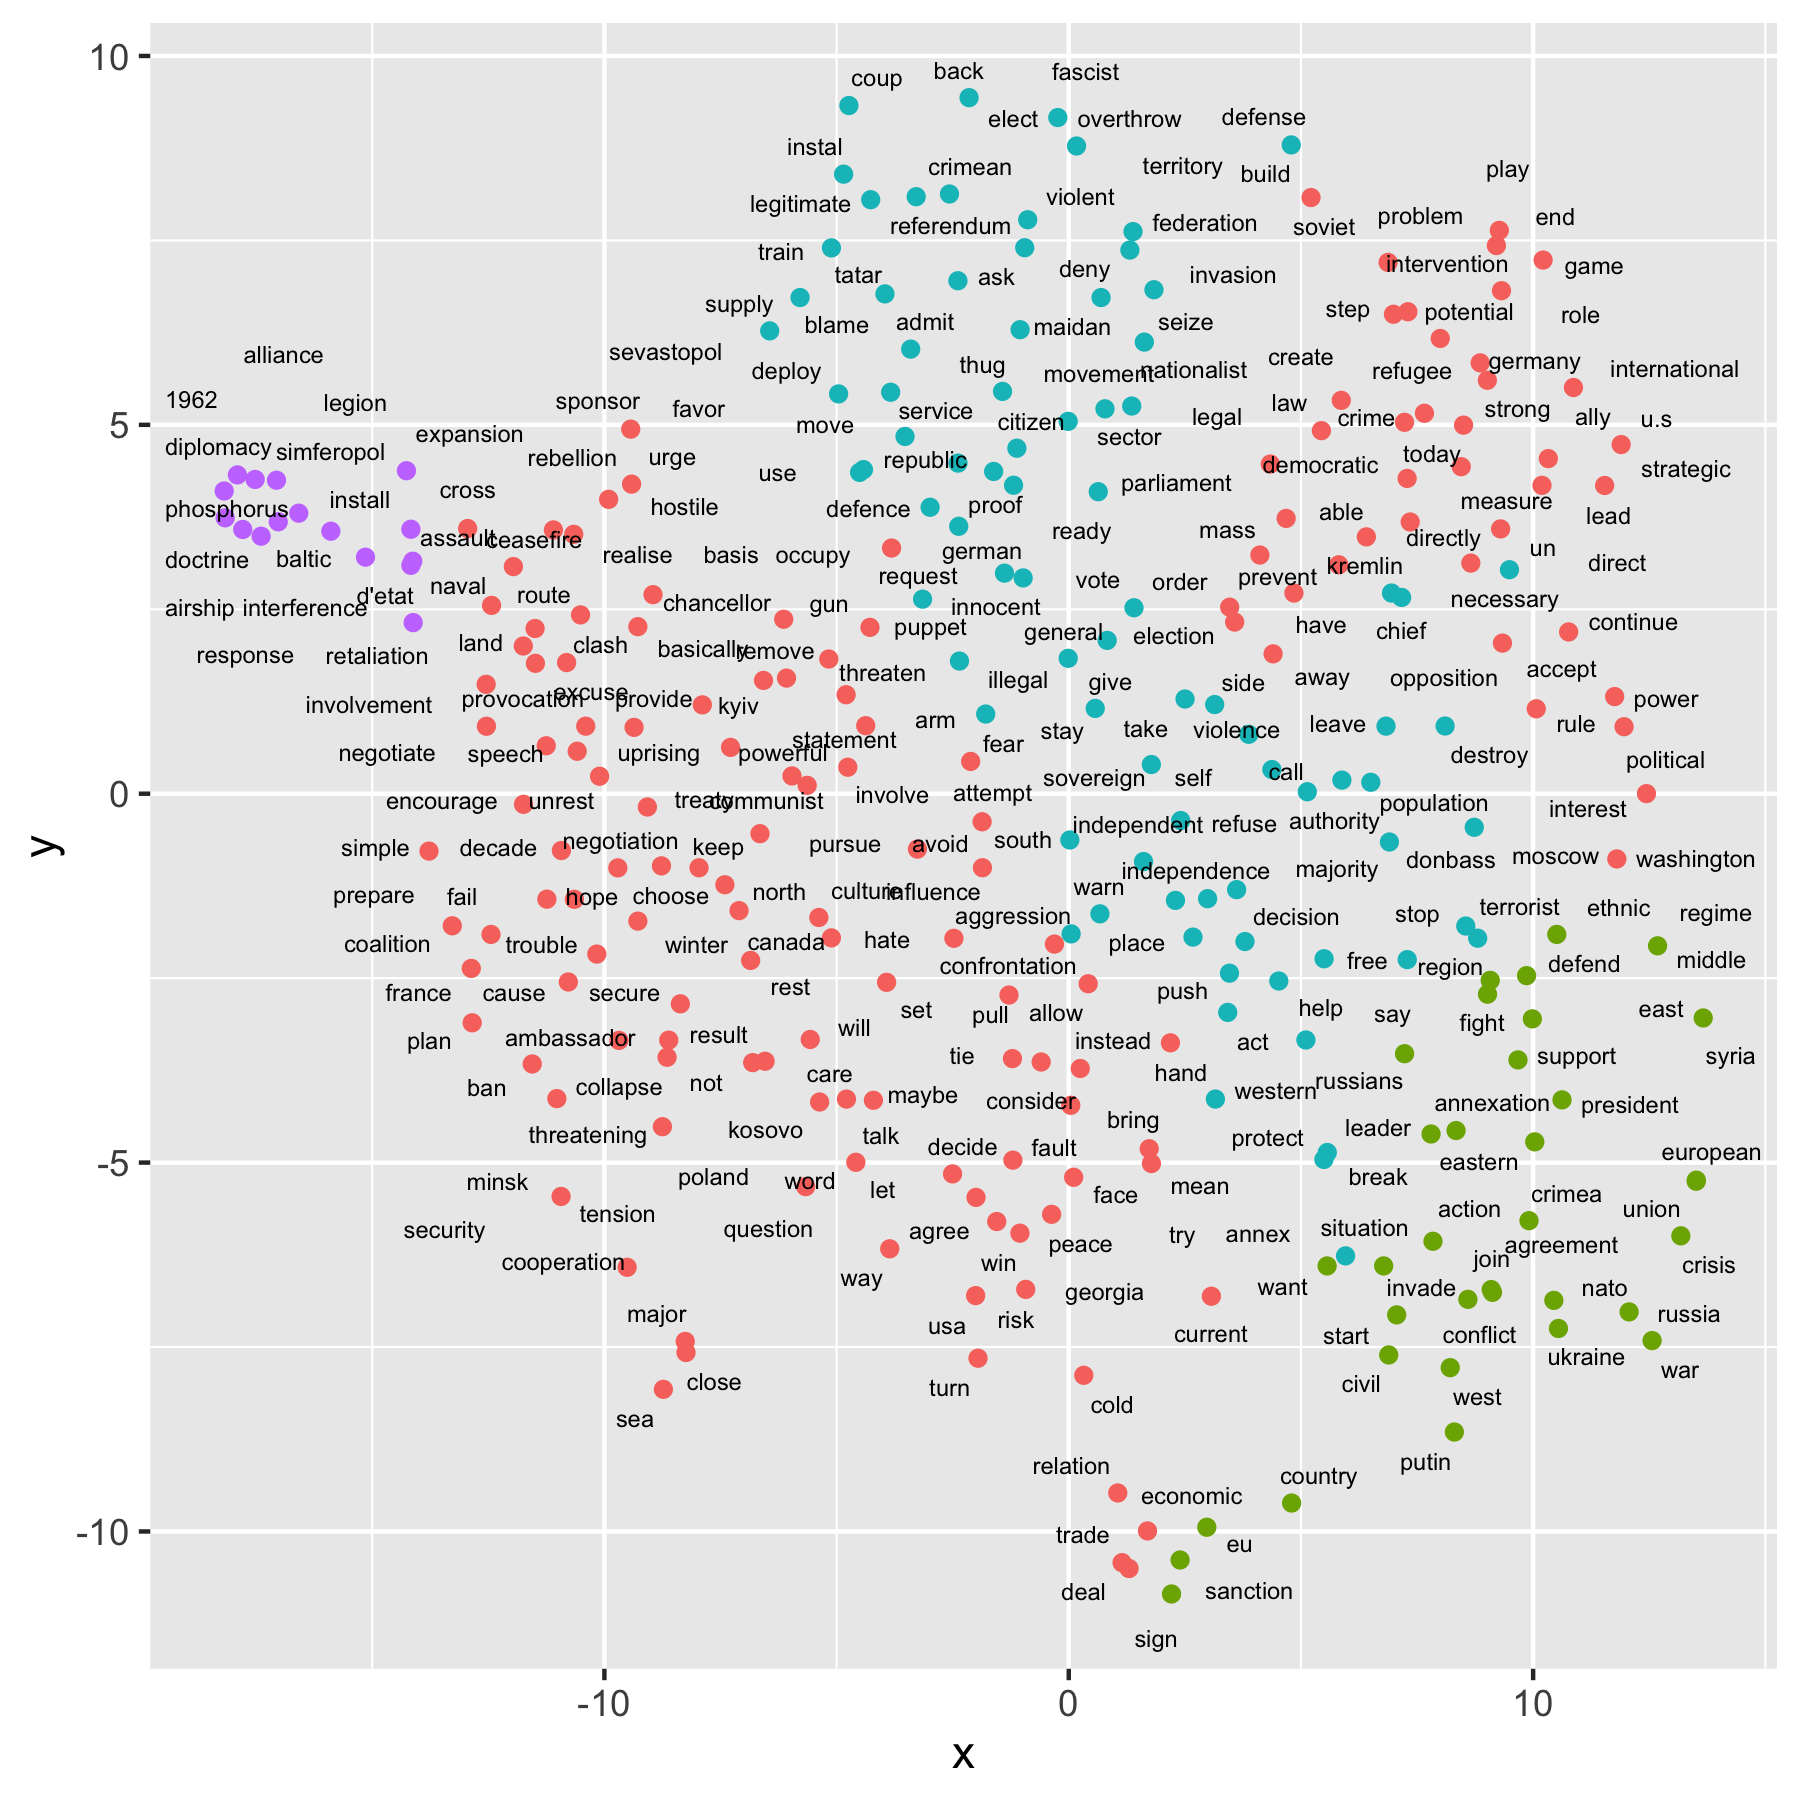
\includegraphics[width=\textwidth]{rus/superspreader_putin}
\caption{Most-similar to ``putin'' (superspreaders)}
\label{fig:superspreader_putin}
\end{figure}

The following figures display the most-similar words for ``putin'' for selected terms across two groups.
In Figure \ref{fig:superspreader_putin}, there are 287 terms; because Word2vec discovers relationships, terms cluster both by ``personness'' and other factors, we remove 13 names of individuals to avoid this.
There is no optimal k for the number of clusters, but the clustering remains similar using various options and the superspreader group presents similar plots using different terms: \emph{putin, crimea, ukraine}.
The term \emph{putin} is located near 8.3, -8.65, its surrounding cluster contains the entities he is in direct competition with: \emph{west, nato, ukraine, european, union, eu}, using various means: \emph{conflict, war, sanction, agreement, invade, defend, fight, support, action, russia}, over objects of contention: \emph{crimea, russians, middle, east, eastern, region, syria}.

The cluster at -15, 2 includes pointed arguments: \emph{1962}, the year of the Cuban Missile Crisis, and claims of \emph{phosphorous}.
Split across -10, -5, and 10, 5 is an international cluster of secondary actors and issues: \emph{france, germany, kremlin, u.s, ally, ambassador, chancellor, poland, kosovo, georgia} and less concrete actions and notions: \emph{speech, provocation, negotiate, encourage, prepare, strategic, prevent, power}.
Finally, the cluster located at 0, 10 is a series of terms that match Russian talking points, painting the new government of 2014 as nazis denying popular will: \emph{coup, fascist, maidan, puppet, nationalist, movement, thug, overthrow, sector, illegal, legitimate, instal, sovereign, independent, referendum, majority, population, donbass}.

\begin{figure}[!ht]
\centering
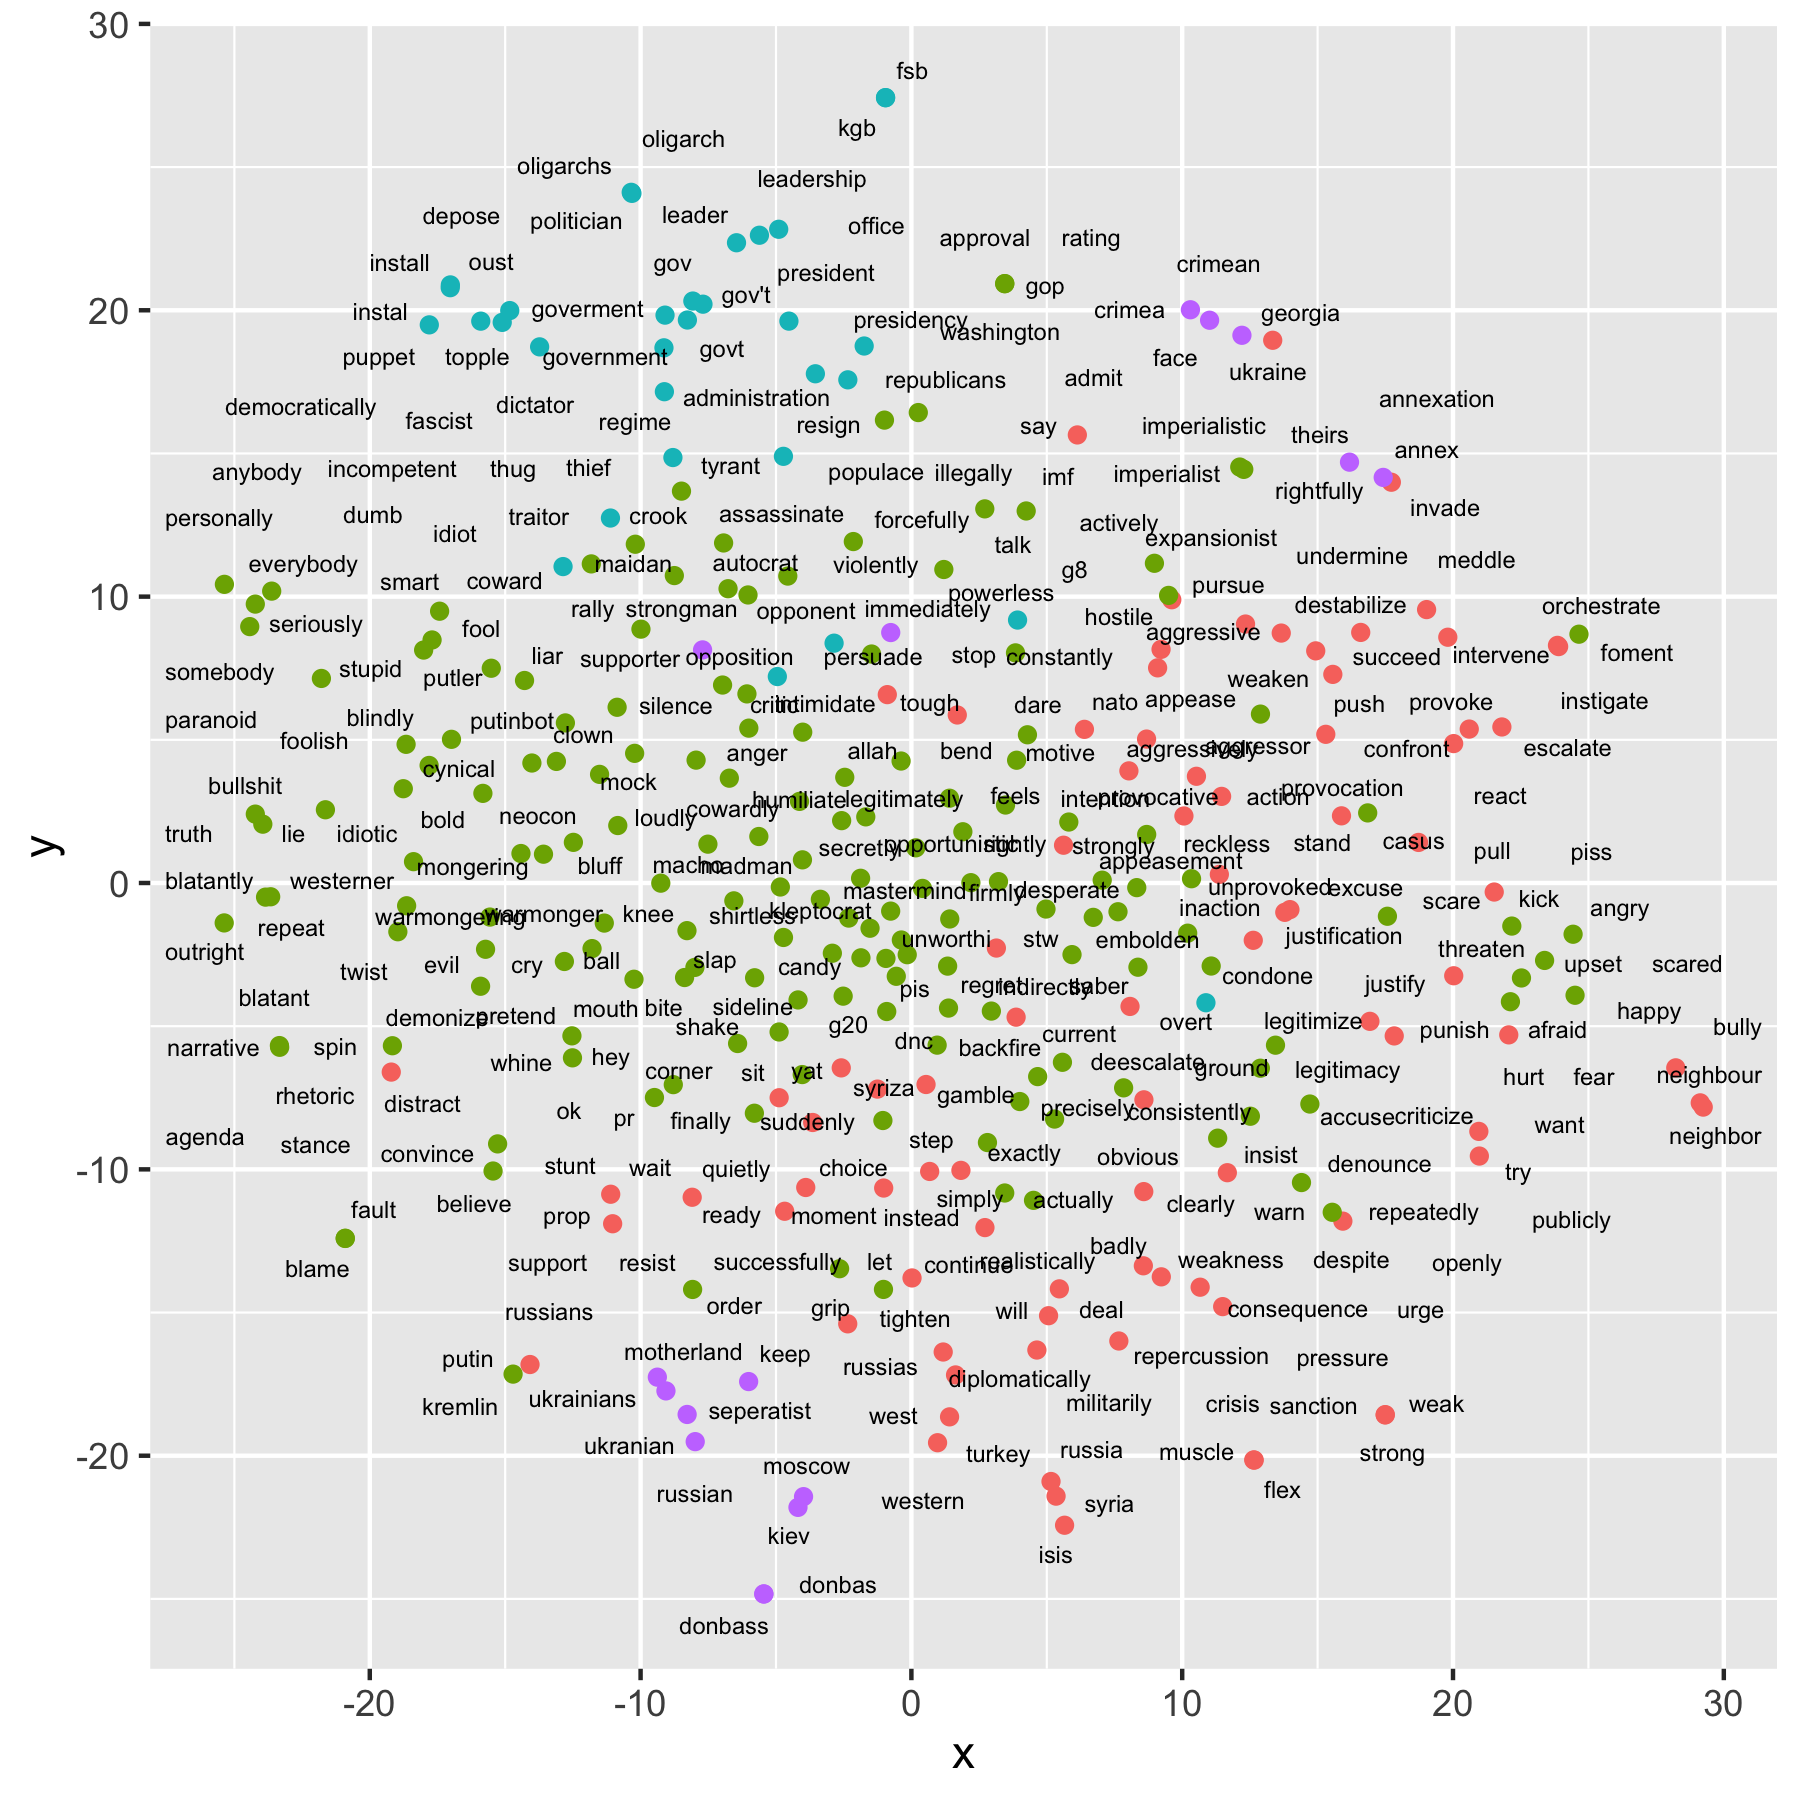
\includegraphics[width=\textwidth]{rus/neutral_putin}
\caption{Most-similar to ``putin'' (neutral users)}
\label{fig:neutral_putin}
\end{figure}

In comparison, the neutral users plot of Figure \ref{fig:neutral_putin} presents similar clusters with a different emphasis.
This group is dominated by individuals; 316 terms are displayed with 84 excluded.
We locate \emph{putin} near -14, -16; nearby is a cluster of relevant parties: \emph{ukrainian(s), moscow, kiev, donbas(s), crimea(n), separatist}.
The international cluster (10, -20) of actions remains, though it tends to be more negative: \emph{pressure, bully, neighbor, hurt, punish, weakness, repercussion, crisis, unprovoked, aggressive}.
Similarly, the cluster at -10, 2 focuses on a puppet government, though it is not obvious to which government it is referring: \emph{puppet, government, topple, fascist, dictator, depose, install, oust, thug, oligarch(s), kgb, fsb}.
The most obvious difference is found in the central \emph{putin} cluster, where the majority of the terms are very negative: \emph{stupid, idiotic, foolish, paranoid, bullshit, demonize, evil, madman, liar, fool, putler, clown, coward(ly), desperate, warmongering}.
Clearly, these different groups display strong differences in narrative and opinion; to determine whether either group is representative of discussion we look at different terms in the top users group.

\begin{figure}[!ht]
\centering
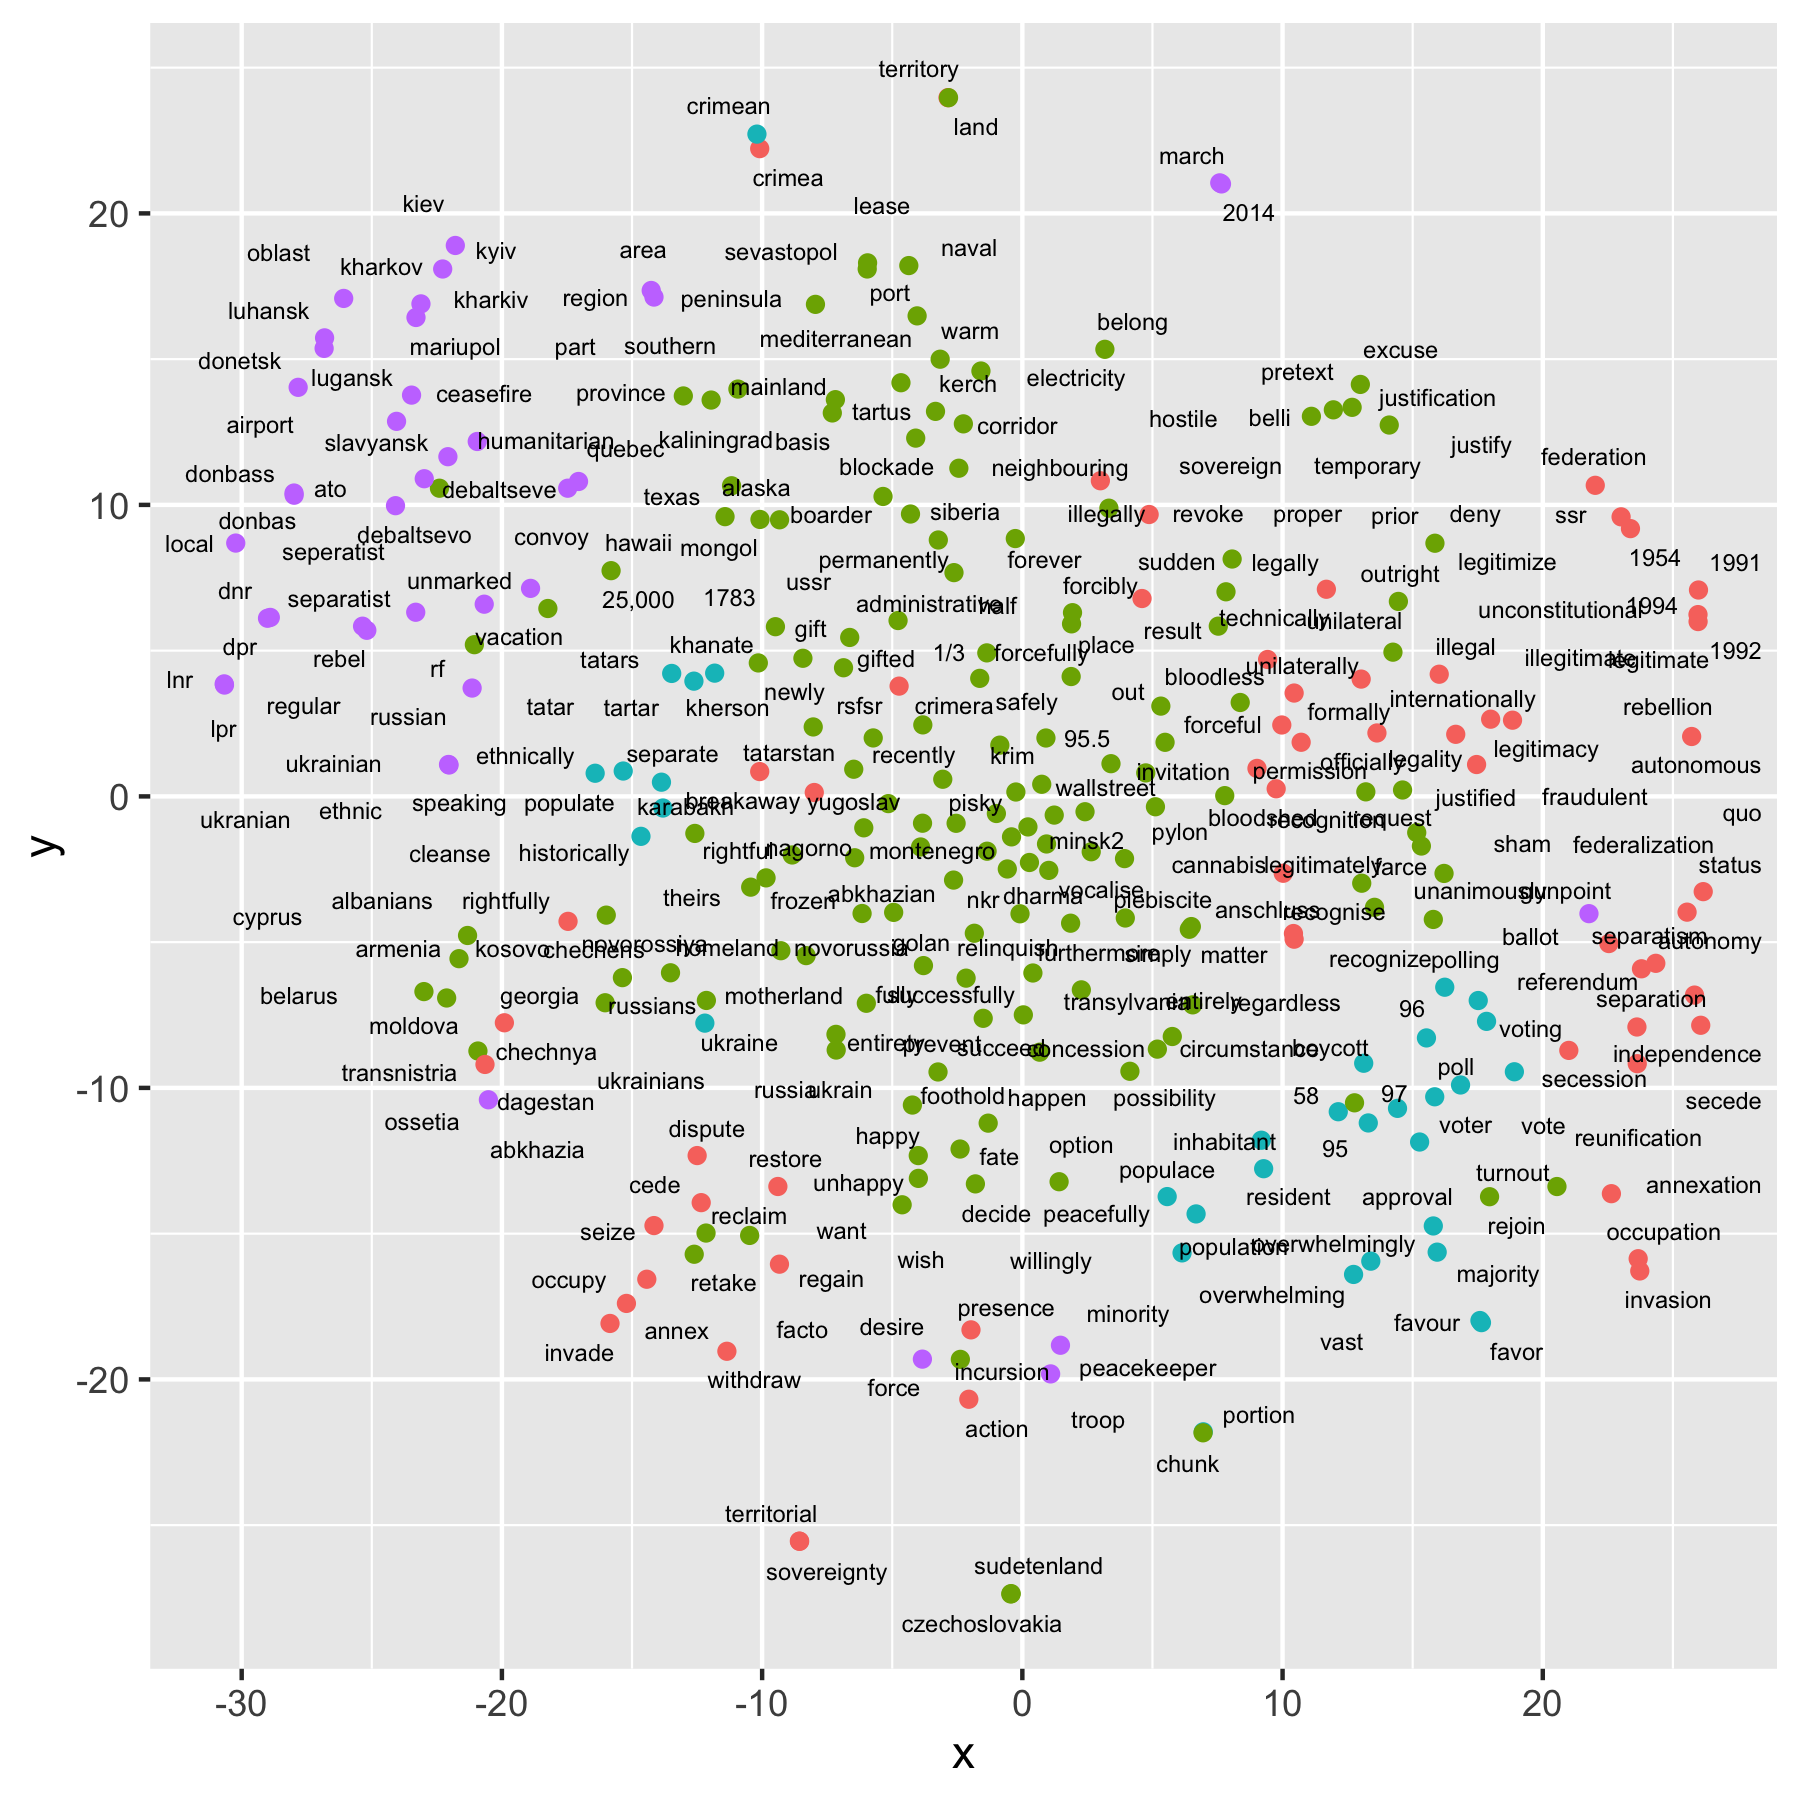
\includegraphics[width=\textwidth]{rus/top_crimea}
\caption{Most-similar to ``crimea'' (top users)}
\label{fig:top_crimea}
\end{figure}

\begin{figure}[!ht]
\centering
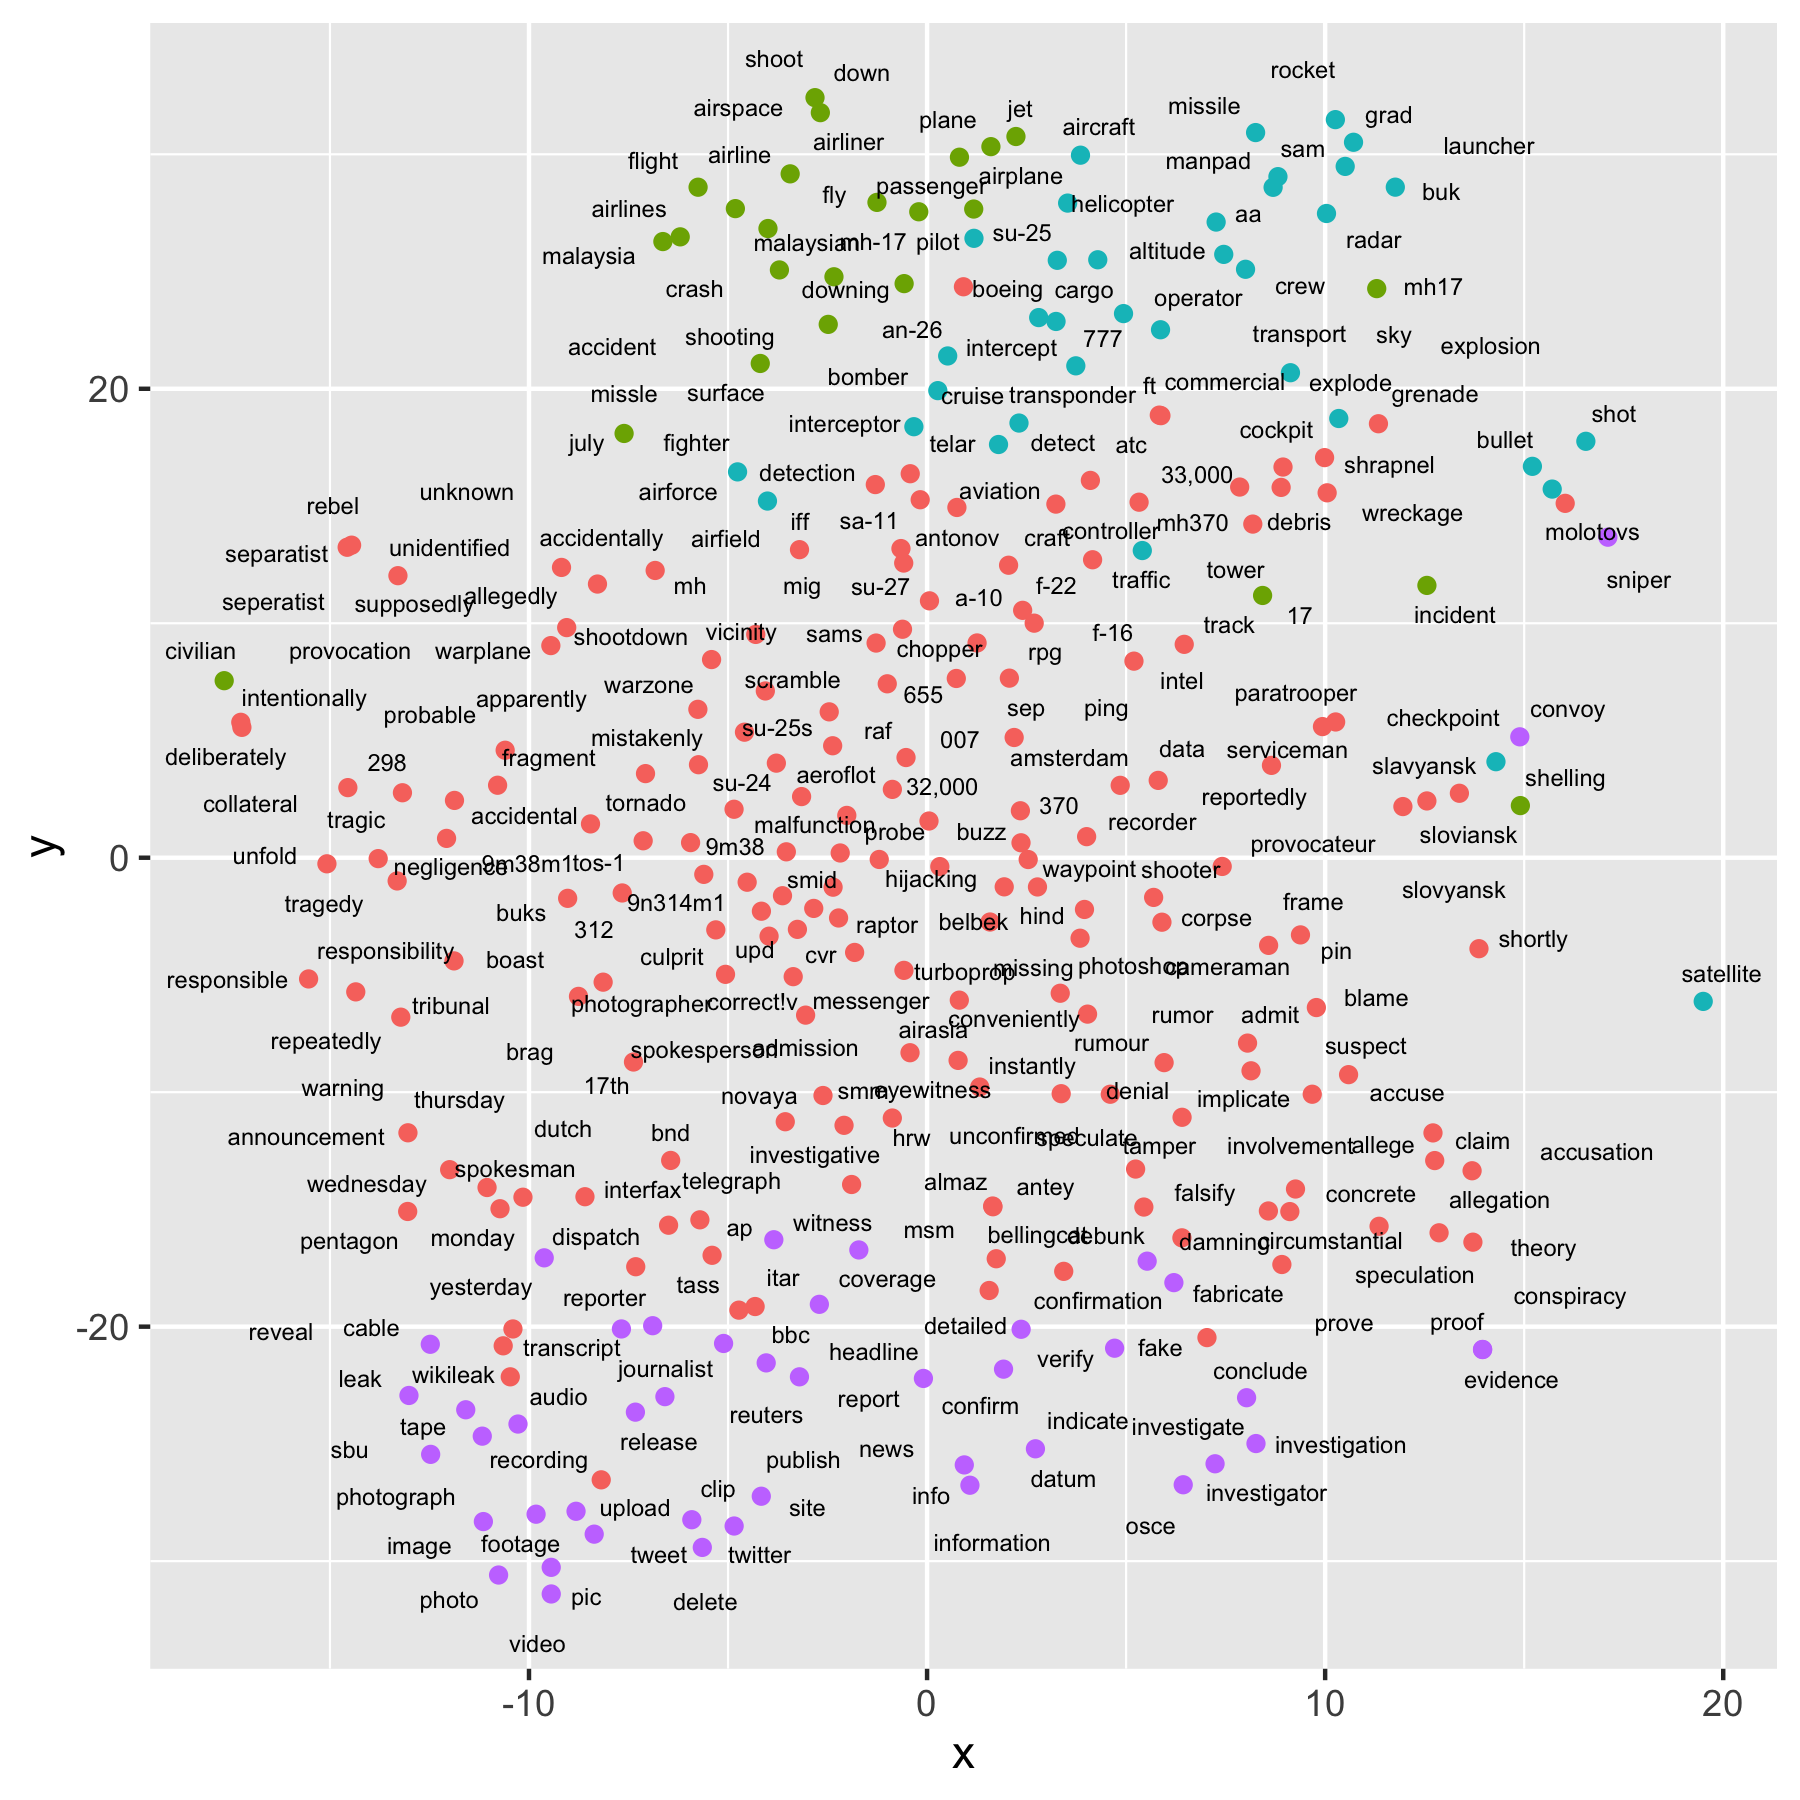
\includegraphics[width=\textwidth]{rus/top_mh17}
\caption{Most-similar to ``mh17'' (top users)}
\label{fig:top_mh17}
\end{figure}

Figures \ref{fig:top_crimea} and \ref{fig:top_mh17} show most-similar terms for the top users group.
The first graph displays the 294 most-similar terms for ``crimea'' with 6 terms excluded.
The cluster at -20, 10 contains the reality on the ground with Russian-backed republics established by separatists in the Donbass region: \emph{separatist, ceasefire, donbas(s), donetsk, luhansk, oblast, march, 2014}.
The term \emph{crimea} is found nearby at -10, 20, but most of its cluster is located at 25, -10 with a discussion of the legalities involved: \emph{secession, federalization, legitimacy, fraudulent, autonomous, unconstitutional, reunification}, relevant years: \emph{1991, 1992, 1994, referendum}, and \emph{1954, ssr}, the year Ukraine was attached to the Ukrainian SSR.
The nearby cluster at 10, -15 continues the topic of voting: \emph{population, populace, willingly, peacefully, overwhelming(ly), vote(r), poll(ing), favor}, reflecting the Russian populace of the region, and at -15, 0, remembering that those demographics were recent: \emph{historically, populate, ethnic, cleanse, tatar(s), khanate}.
The last cluster at 0, 0 has a similar historic tilt: \emph{1783, novorussia, warm, port, sevastapol}, and transparent attempts to connect the annexation of Crimea to other historic annexations and existing independence movements: \emph{hawaii, texas, alaska, kosovo, quebec}, yet also contains more recent, more negative analogs: \emph{sudetenland, anchluss, czechoslovakia}.

In Figure \ref{fig:top_mh17}, there are 286 terms with 14 excluded; ``mh17'' is found near 10, 25, its cluster is at -5, 25 with a straightforward account: \emph{malaysia, airlines, accident, shooting, downing, crash}.
The cluster at 5, 25 gives more details: \emph{buk, missile, sam}, the Buk was the Russian-supplied missile system used by separatists (probably commanded by Igor Girkin) to destroy the plane.
The cluster found at 0, -10 is concerned with the investigation: \emph{image, photograph, footage, clip, site, report, bbc, itar, reuters, tweet, twitter, journalist, transcript, confirm, evidence}, as is the main cluster located at 0, 0, with the \emph{dutch} investigative team that confirmed the separatist shoot down as well as \emph{bellingcat}, an investigative team dedicated to debunking misinformation.
Distributed around the cluster is the \emph{conspiracy theory} given by the supposed \emph{traffic controller} at an \emph{airfield tower} in Ukraine that saw an Ukrainian \emph{su-24} in the \emph{vicinity} of the shoot down, an account promoted by Russian media.

For the Putin plots, both superspreaders and neutral users contain abstract terms related to Putin himself as well as a variety of details about the Ukrainian and Crimean conflict.
The biggest and expected difference is in the many negative references found in the neutrals but missing from the superspreaders

In comparison, the plots of the top users (or users that are getting responses), while including relevant details also contain a large number of terms related to Russian talking points.
For example, the many dates and references to annexation in the Crimea plot and stories distributed by the Russian MoD and media regarding MH17.
This mixed group of active discussion we might expect to be less colored than the actual Russian superspreaders is instead the most-framed.
It makes sense that the act of communication and debate between two groups brings out more information, this suggests that the best way to combat disinformation is not to target ideological groups but rather to ensure valid, factual information is there to counter the misleading when discussions happen.

\section{Discussion}

In this chapter we discussed how a combination of dynamics - the fall of the Soviet Union, rise of the Putin regime, and growth of the tech industry across the world led to an embrace of computational propaganda by the Russian government.
Computational propaganda was combined with asymmetric warfare, covert operations such as poisonings, and hacking and misinformation campaigns to produce the so-called Gerasimov doctrine.
This was first tested at scale in Ukraine from 2013 to 2014 leading up the the Crimea's annexation by Russia.
We use the existing academic literature about this crisis and general tactics of Russian ``trolls'' across social media including Facebook and Twitter in order to guide our analysis of the crisis using the Reddit dataset.

We clean the dataset, process it using spaCy, then use a basic filtering scheme checking for the presence of terms like ``putin'' and ``crimea'' to find matched and related items.
The dataset is further filtered using a set of rules regarding subreddits in order to exclude irrelevant data.
The resulting data shows spikes in activity corresponding closely with the main events of the crisis - the abdication of Yakunovych and annexation of Crimea, the downing of MH17, and the Minsk II ceasefire.

Next, we use a simple categorization scheme using web domain addresses in order to put content and users into neutral and pro-Russian groupings, filtering out apparent bots.
This involves a combined list of ``core'' Russian (and Chinese/Iranian) state-owned domains and outlets and an ``extended'' list of domains across the political spectrum known for parroting Kremlin talking points or conspiracy theories, some more covertly or intentionally than others.
Users with at least 10 cites of a domain in this list across the 3 years are known as ``spreaders'' of pro-Russian content and those with more than 25 are ``superspreaders''.
We find that while discussing this topic users generally cited a variety of US, British, Ukrainian, other international, and Russian outlets with Russian state media being prominent.
Pro-Russian users seem to favor niche, low-credibility sources.
Users cited Wikipedia more than any other domain with many references to analogous historical events.

In order to observe patterns in activity as well as the possible reach of the pro-Russian users, we use several methods from graph theory and network analysis.
The first, k-core analysis, confirms the presence of pro-Russian users in the highest shells of users with the most connections to other users in the network, with spreaders and superspreaders found heavily clustered in the top k-core.
These same superspreaders similarly dominate top measures of betweenness centrality and total degree (number of connections) and show an apparent preference for a handful of subreddits and for citing Wikipedia.
These various measures suggest that pro-Russian propaganda has achieved positions of influence in the network, allowing for easy dissemination.

Finally, we train our own Word2vec models.
By training separate models for different groups of users we are able to compare word associations of a given term across them.
This is achieved by dimensionality reduction in order to plot terms on a two-dimensional graph with points clustered via k-means.
In the case of the term \emph{putin}, neutral users present a cluster of negative terms which is absent for the superspreaders.

These different groups show a different focus, but to capture which narratives dominate the average discussion, we create a final group of ``top users'', containing only items that have at least a single reply.
Both \emph{crimea} and \emph{mh17} include clusters with straightforward accounts as well as a relatively nuanced description of various connected issues.
However, these accurate accounts are distributed among pointed historic and legal arguments, as well as conspiracy theories promoted by the Russian state.

We note the apparent effectiveness of the framing of these issues - the exact same event or notion can be used to support wildly different positions.
Whether framing in this data is the result of an intentional campaign or just obsessive users is difficult to say, though users including u/vigorous post an unusually high number of items.
We note the apparent presence of power laws in the dataset.
Zipf's law, commonly applied to textual data, says that in a large enough body of text the term used most frequently will be used twice as often as the second most used term, three times as often as the third, and so on; or, the frequency of a term is inversely proportional to its rank.
Zipf has been more generally applied to other human interactions, this clustering activity seems to be a feature of human behavior.
The practical result of most discussions being limited to a few subreddits, most citations involving the same domains or articles, and a relatively limited number of topics means that it would take very few users to control and direct discussion, to have outsized influence.
Compounding this is the difficulty of knowing what varied demographics with their own beliefs, biases, and knowledge bases will notice and prefer when presented the average Reddit thread, news article, or equivalents of clusters of terms.

The end result of this chapter has been the development of a general framework for filtering and categorizing a large textual dataset.
For any group of users across any topic we can distill the combined text into a visualization of several hundred words, graphs of talking points.
Next, we apply this framework to the 2016 US presidential election.


\chapter{usprop: The 2016 Presidential Election (2015-2017)}
\epigraph{Nations reel and stagger on their way; they make hideous mistakes; they commit frightful wrongs; they do great and beautiful things. And shall we not best guide humanity by telling the truth about all this, so far as the truth is ascertainable?}{W. E. B. Du Bois}

\section{Introduction}
The previous chapter provided a foreign, international case study of pro-Russian superspreaders and their influence on discussion over the Crimean invasion and following conflict.
The Mueller Report, discussed shortly, gives details of a sustained  computational propaganda campaign that engaged with and supported both progressive and conservative causes during the 2016 presidential election.
Besides this foreign interference, the presidential election draws the most coverage and interest of all elections in the United States.
Furthermore, the United States has a history of using new communication technology in campaigns and an active press.
Given that we should expect more partisan activity during presidential elections, what did progressives and conservatives discuss during the 2016 election?
Do the narratives in these discussions match reality or is are they distorted and biased?

Social media is only the leading edge of communication technology, one largely developed within the United States.
The United States, as an open, capitalist democracy has had an outsized impact on the development and commercialization of communication technology during the last two centuries, political adoption has quickly followed.
In this chapter we take a wide scope, hoping to capture the very gradual global development of these tools throughout history.
From the printing press to Twitter, communication has made the world of today feel much smaller than it has been historically and our benefit of hindsight presents a simple narrative of progress which in reality was the emergent result of many interacting cultures over time, an abstract social network.
Correspondingly, the following describes how the political systems of the United States and Russia differ due to an accumulation of historic factors, these old events giving narratives their power.

\subsection{The Mueller Report: Conspiracy, Coordination, Collusion?} 

On March 22, 2019, The Report On The Investigation Into Russian Interference In The 2016 Presidential Election or ``Mueller Report'' was delivered to US Attorney General William Barr \cite{nyt-2019}.
Two days later, Barr sent a four-page summary (the Barr letter) to Congress with the Justice Department's conclusion that there was not sufficient evidence of coordination with Russian operatives during the 2016 election or obstruction of justice by Trump and his associates to warrant further action \cite{barr-2019}.
Mueller criticized Barr's summary as failing to ``capture the nature, context, and substance'' of the 448-page report, leading to ``public confusion'' \cite{wp-2019}.
The report was released with redactions to the public on April 18, 2019 \cite{cnbc-2019}.

Robert Mueller was appointed Special Counsel after Trump dismissed Director of the Federal Bureau of Investigation, James Comey, while Comey and the FBI were investigating Trump and his associates for connections with Russian officials.
Special counsels are appointed when there is a conflict of interest, the most prominent example is Watergate.
Mueller was given authority to investigate connections between Trump associates and Russia, whether Trump obstructed justice with Comey's dismissal, and whether there was Russian interference in the 2016 election \cite[p.11]{mueller}.

Volume 1 of the report details how the Internet Research Agency (IRA), funded by Yuri Prigozhin, in 2014 began a social media campaign of ``information warfare'' and ``active measures'' that were ``designed to provoke and amplify political and social discord in the United States''.
That year IRA employees made trips to the US and obtained information and material used in a campaign aimed at undermining the electoral system.
By 2016, their efforts shifted focus to supporting Sanders and Trump while attacking Clinton; party infighting and a Trump presidency being favorable to Russian interests \cite[p. 14]{mueller}.

Their tactics involved ``specialists'' representing themselves as American individuals and organizations across the political spectrum on various social media websites \cite[p.22]{mueller}.
During 2016, the IRA purchased more than 3,500 ads on Facebook worth \$100,000 to promote causes supported by botnets across platforms: ``United Muslims of America'' had over 300,000 followers, ``{Don't Shoot Us}'' over 250,000, ``Secured Borders'' over 130,000, and, on Twitter, @Pamela\_Moore13 over 70,000. 
US media outlets quoted IRA accounts; Donald Trump Jr., Eric Trump, and Kellyanne Conway cited or retweeted @TEN\_GOP; Roger Stone, Sean Hannity, and Michael Flynn interacted with the same account; Donald Trump's personal account responded to @10\_gop, an alias of the deactivated @TEN\_GOP. 
As of January 2018, Twitter had disclosed 3,814 IRA accounts posting 175,993 tweets in the 10 weeks leading up the the 2016 election; by August 2017 IRA Facebook accounts made over 80,000 posts reaching at least 29 million ``U.S persons'' and up to 126 million people \cite[pp. 26-28]{mueller}.

Fake personas organized dozens of rallies in the US, some with hundreds of attendees throughout 2016, but failed to get official support from the Trump campaign, despite multiple attempts.
These measures were combined with the hacking of members of the Clinton campaign and the Democratic National Convention by Russian intelligence (GRU) using methods like spearphishing - an email disguised as password reset giving unintended access \cite[p.29-37]{mueller}.
This and Clinton-related material was leaked during the campaign by the personas of DCLeaks and Guccifer 2.0, both tied to GRU \cite[p.41]{mueller}.
These personas had repeated contact with Julian Assange; WikiLeaks would twice release this material within hours of the revelation of Trump scandals, and would continue to suggest that the source had been Seth Rich, murder victim, despite knowing otherwise.
GRU similarly gained access to and installed malware on networks of individuals and organizations involved in local and state elections, voting-technology companies, and voter databases \cite[p.46-51]{mueller}.

The report summarizes, ``the Russian government interfered in the 2016 presidential election in sweeping and systematic fashion''.
While political rhetoric is often intentionally obtuse, legal rhetoric by nature should be precise.
The jargon of the report lends itself especially to misrepresentation, using legal terms which have different meanings in a popular, public context.
Collusion is not a ``term of art'' in federal criminal law, but multiple parties involved with the social media campaigns and hacking have been charged with and convicted of conspiracy and other felonies. 
There was no conclusive evidence that the Trump campaign coordinated, or had an agreement with Russian officials, but there was extensive communication and apparent attempts to hide this interaction \cite[p.2-9]{mueller}.
In the case of the IRA social media contacts, there were no charges due to a lack of evidence that anyone that coordinated or communicated with them were aware they were fake US personas operated by Russian specialists \cite[p.35]{mueller}.
However, the Trump campaign welcomed the illegal foreign election interference they were aware of and former National Security Advisor Michael Flynn and Trump campaign chairman Paul Manafort pled guilty to lying about their interactions with Russians \cite[p.9-10]{mueller}.
The report makes no judgement on competence, but it is clear that officials and citizens across the political spectrum were duped throughout the 2016 election cycle using domestic corporations and technology.

\subsection{History}

To understand American political development up to 2016, it is useful to go further back into Russian history.
The states known today as Russia, Belarus, and Ukraine began with the Kievan Rus' polities founded in the 9th century.
The earliest historical source we have of these events is the Primary Chronicle, part history, part legend, written more than a century later of ``bygone years'', not unlike other national epics like the Greek Iliad, Hebrew Bible, or Persian Shahnameh.
Scandinavian Norsemen, known as Varangians, traded with, settled among, and raided the Baltic and Eastern Slavic tribes that lived along the rivers between the Baltic and Black seas.
In the Chronicle's account, the Varangians were driven out by locals whom then fought amongst themselves, leading to their request of the Scandinavians to return under Rurik and his brothers as rulers.
He supposedly took power in Novgorod; certainly and gradually the Varangians Slavicized and adopted local customs, creating a unique ethnicity and culture, the Rus'.
Rurik, said to have died in 879, may not have existed, but the Rurikids remained the ruling dynasty of Kievan Rus' until 1598 \cite[p.1-4,53]{bushkovitch2011}.

The Rus' traded as far east as Baghdad and raided as far south and east as Persian and Turkic settlements near the Caspian Sea; in 860, they attacked Constantinople. 
This raid was led by the founders of Kiev, according to the Chronicle. 
Due to geography the Byzantine Greeks and Rus' made natural trading partners and competitors; Constantinople would be attacked on at least two other occasions over the next century, but treaties were signed and relations normalized \cite[p.41-52]{gleason2009}.
The eastern Church sent missionaries among the Slavs, and Igor of Kiev's wife, Olga, converted and served as regent after his death.
Her son, Sviatoslav, in 965 defeated the Khazars, a unique Jewish Turkic state and basis for modern anti-Semitic theories.
His son, Vladimir the Great, converted to Christianity in 988 and married the Byzantine Emperor Basil's daughter, Anna, cementing the eastern European ties of the Rus' \cite[p.6-8]{bushkovitch2011}.
That year Vladimir sent 6,000 men to help Basil quell a revolt; Basil, not trusting the loyalty of his own men, formally established this Varangian Guard as the emperor's personal bodyguard \cite{gleason2009}.

In this same era, the Norsemen that headed west became known as Vikings.
Repeated raids up French rivers and on Paris led to a peace treaty in 911 in which the Viking Rollo became Duke of Normandy, a vassal of the King of France, and was baptized.
His descendant William conquered England in 1066 and this Norman elite eventually blended with existing waves of Anglo-Saxon, Viking, Roman, and Celtic inhabitants to form a unique ethnicity and culture, the English \cite{rowley2022}.
It was from Western Europe that the United States took its political culture and the WASP (White Anglo-Saxon Protestant) core until recently acted as owners and custodians of political power, now challenged (and evolving) due to new media.

Norse settlement extended as far west as Greenland and Newfoundland in the 11th century.
Normans ruled portions of Scotland and Ireland, captured Sicily and Malta, ended Byzantine rule in southern Italy, established states in Antioch in Syria and on Cyprus during the Crusades, and took part in the Reconquista in Spain \cite{rowley2022}.
Descendants of Scandinavians had similar cultural origins but over time the orientation of the former Vikings to the west and the once Varangians to the east created strong distinctions.
The split between the western Catholic church and the eastern Orthodox church in 1054 along not only confessional but also political, linguistic, and national lines is an early example of this European divide obvious even today \cite[p.8-9]{bushkovitch2011}.

This more general process of a nomadic and military elite being assimilated by a native population into new synthetic cultures is common.
The Bulgars similarly Slavicized, the Magyars (Hungarians) kept their language, Anatolia and large parts of Central Asia Turkified, Turkic tribes and the Mongols of the Ilkhanate Persianized, and the Mongols of Kublai Khan established the modern capital at Beijing, in time becoming China's Yuan dynasty \cite{golden1992}.

The Rus' states under the Rurikid princes were also defeated by the Mongols. Kiev was razed in 1240, and for hundreds of years the Golden Horde dominated while the Rus' were devastated by their armies and heavy taxation.
During this time Kiev, Novgorod, and other cities lost power, Moscow rose to prominence in the northeast, and the Rus' began the divide into their modern nationalities \cite[p.19-23]{bushkovitch2011}.

In 1533, when Ivan IV (the Terrible) became Grand Prince of Muscovy, his territory was an isolated and unknown country between the Dnieper and Volga rivers.
He conquered khanates to the east, was crowned tsar in 1547, and expanded Russia to the Ural Mountains \cite[p.47-50]{bushkovitch2011}.
To the south, from the plains of the Eurasian steppe, Tatars made regular raids deep into Russian territory along the Muravsky, Izyumsky, and other ``trails'', and in 1571 Moscow was burned with tens of thousands of Russian victims and prisoners \cite[p.264-277]{madariaga2006}.
Raids continued into the 18th century and were not completely ended until the annexation of the the Wild Fields of Ukraine and Crimea during the reign of Catherine the Great. This area eventually became ``Novorussia'' through an influx of settlers and construction; the Donbas (Donets Basin) became an industrial center in the late 19th century \cite[p.109,122]{bushkovitch2011} \cite{sunderland2004}.

Despite or because of similar threats, the tsardom and then empire began a slow, continuous expansion to the west further into Europe, east towards the Pacific Ocean, and south to the Caucasus Mountains, Central Asia, and Black Sea.
Yermak Timoveyevich led the first campaign into Siberia in 1582; after 1613, Russia grew at a rate of 20,000 square miles per year \cite[p.53]{bushkovitch2011} \cite{montefiore2017}.
Russian settlement reached its furthest extent on the Pacific at Fort Ross in 1814, 90 miles from today's San Francisco.
The Russian-American Company operating the fort sold it to John Sutter in 1841, seven years later gold was found at another of his properties beginning the California Gold Rush \cite{parkman1996}.

This Russian expansion mirrors that of the United States from isolated settlements to an empire touching the Pacific, overwhelming people groups on either side of the Bering Strait.
However, their political institutions developed very differently, even though
Russians were aware of democratic forms of governance.
Novgorod was a republic with a popular assembly that elected a prince from among the boyars \cite[p.12]{bushkovitch2011}.
Peter the Great opened the country to western Europe, founding Saint Petersburg in 1703 on the Gulf of Finland, and the empire consumed states with democratic traditions  such as the the Cossacks of Ukraine and Polish-Lithuanianian Commonwealth in the 18th century.
Despite these influences, it remained a monarchical state dominated by a limited nobility, even more authoritarian than most other European monarchies of the time \cite[p.28, 65]{bushkovitch2011}.
The Emperor adopted the term autocrat from the Byzantine Greeks, emphasizing the absolute power of the sovereign to lead and protect the Orthodox Church and its followers, Russian people, and Slavic nations \cite[p. 39]{bushkovitch2011}.
This responsibility and justification was used throughout the 19th and 20th centuries, leading to the Crimean War (1853-1856) and repeated conflict in the Balkans and southeastern Europe \cite{montefiore2017}.

When Napoleon's invasion of Russia failed in 1812, Russian forces captured Paris and at the Congress of Vienna in 1815, the Russian Empire became a recognized great power that kept stability through the Concert of Europe and the Holy Alliance.
In this role, the Emperor Nicholas became known as the gendarme (policeman) of the continent.
His first act was to end an attempted coup by reformist officers known as the Decembrists in 1825, he put down a rebellion and abolished the constitution of Poland in 1830, then Russian forces were requested to crush a liberal revolt in Hungary in 1849 \cite[p. 149-166]{bushkovitch2011}.
Lincoln captured liberal sentiment in 1855 while writing of slavery and the anti-immigrant Know-Nothing party: ``When it comes to this I should prefer emigrating to some country where they make no pretense of loving liberty – to Russia, for instance, where despotism can be taken pure, and without the base alloy of hypocrisy.'' \cite[vol. 2, p. 323]{lincoln2008}

Yet Russia was slowly modernizing and liberalizing; in 1861, Emperor Alexander II freed the serfs from being tied to the land, ending an outdated, ancient feudal system which had limited industrialization \cite[p. 189-192]{bushkovitch2011}.
In the United States, the first transcontinental railroad was finished in 1869, while the Russian Trans-Siberian railway opened in 1904, connecting Europe to the Pacific \cite{bowman1957}.
Due to its large population and material resources, the country always had great wealth, but mass industrialization changed the economy and society as the coal, iron, steel, textile, and petroleum industries became some of the largest in the world (the fortune that funded the Nobel prize came from the oil fields of Baku) \cite[pp. 837-844]{portal1965}.
Saint Petersburg would double in population between 1890 and 1914 as people flocked to the cities to join a growing working class; nearly 30\% of factory workers were women \cite[p. 208-227]{bushkovitch2011}.
Defeat in the Russo-Japanese War in 1905 forced Nicholas II to establish a representative legislature, the Duma \cite[p.269,211]{bushkovitch2011}.
Though it had only been ruled by Rurikids and Romanovs for more than a thousand years, by the start of World War 1, few countries had faster economic growth or more political potential than Russia.

\subsection{The Federalist Papers}

Political evolution in the United States was to a much greater extent by intentional design.
The founding generation Lincoln called the ``patriots of seventy-six'' had this Russian and other political histories as a context and guide when putting together the Constitution seventy years earlier \cite[vol. 1, p. 112]{lincoln2008}.
Some of the best material we have on the thinking behind its design can be found in The Federalist Papers.
Part descriptive, part persuasive, the papers were in total 85 essays written by Alexander Hamilton, James Madison, and John Jay as ``Publius'' published between October 1787 and the summer of 1788 in New York newspapers in support of the ratification of the Constitution \cite[p. 2]{mosteller2012}.
Though not a complete picture of popular political views at the time, this outcome of the convention of 1787 was ratified by the states the next year.
The primary arguments against the papers came from a number of essays, several by ``Brutus'' and ``Cato'', which would years later be collected as ``The Anti-Federalist Papers''.
Despite losing the overall argument, their main contribution was a stand for a Bill of Rights; George Clinton, vice president under Jefferson and Madison, was one notable writer \cite{borden1965}.

The Federalist Papers make clear the necessity of revising the existing confederacy of states established after the revolution, in particular strengthening the federal government by giving it the power to raise taxes and army, and to act as a separate but not dominant power over the state governments.
Shay's Rebellion of 1787, led by a Revolutionary War veteran over high taxes and nonpayment was only put down after a private army was raised.
Federalist 1 poses this event as proof of the failure of the existing government and presents two options: either the Constitution would be ratified or inevitably the states would form separate regional confederacies \cite[n. 1]{fed}.
Washington, who admired and had followed the example of the Roman dictator Cincinnatus returning to work on his farm, was thought to be considering a third option, constitutional monarchy \cite[ch. 3]{feldman2017}.

Washington's motives are understandable though the lens of papers.
They are a model of how the founders perceived the world as well as their audience, those eligible to vote.
Following the Greek and Roman traditions of criticizing Athenian democracy, the distinction is made between the ``true principles of republican government'' and democracies \cite[n. 1]{fed}.
Democracies are defined as states where individuals directly vote on issues and are limited to small geographical areas (today's ``direct democracy'');
republics are states where voters elect representatives and smaller states are bound together into a greater whole.
The term ``confederate republic'' is borrowed from the political theorist, Montesquieu \cite[n. 9]{fed}.

The democracies of Greece and the maritime states of Italy are described as having been ``in a state of perpetual vibration, between the extremes of tyranny and anarchy'' due to infighting \cite[n. 9]{fed}.
Within small states it takes small amounts of influence and power to gain control, by increasing the pool of representatives and size of the state, ``true'' republics improve the quality of the people governing, disperse and redirect factional conflicts, and ``refine'' public views \cite[n. 2, 10]{fed}.
The smaller states within the larger republic receive the advantages of internal standardization and limit petty intranational conflicts and, more importantly, present a united front to outside powers, military and commercial.
Echoing an understanding of the necessity of the sovereign via Hobbes and Locke, this republic is said to have the external advantages of a monarchy \cite[n. 9]{fed}.

The founders were familiar with analyses of government going at least as far back as Plato's \emph{Republic} in which pure democracy, or the inevitable rule by sectarian demagogues, was only preferable to tyranny \cite{plato}.
Cicero's \emph{De re publica}, modeled after the former work, praised the late Roman republic's mixed government \cite{cicero}.
Polybius, a Greek historian writing in the 2nd century BCE, similarly lauds Rome's mixed constitution (the Senate and the people) and separation of powers \cite{polybius}.
Of this knowledge ``imperfectly known by the ancients'', the papers consider distribution of power into distinct departments, legislative checks and balances, courts with accountable judges, and representative legislatures as either ``wholly new discoveries'' or primarily modern advances.
They make no claims about the value of a written constitution but note that ``the science of politics'' had made much progress since the times of the Romans \cite[n. 9]{fed}.

The confederate republic is an advantage in foreign affairs by elevating the stature of the state, the operation of government, and those chosen to operate it.
``Safety from external danger is the most powerful direction of national conduct'', however, considering the country's ``insulated'' geographic position, external danger would most likely result from internal instability caused by faction.
States in constant conflict require standing armies for national defense, the ``military state becomes elevated above the civil'', and citizens view the military as superior.
The greatest danger of this happening is not from foreign powers, but due to the splintering of the union; the resulting smaller confederacies European powers would play against each other \cite[n. 8]{fed}.

To defend against this, the Constitution was designed with multiple failsafes including seperation of powers, checks and balances, and overlapping forms of representation in the houses of Congress.
The geographic size of the republic is another, the hardest to overcome.
If a section of the union experiences abuses of power, popular insurrection, or a ``religious sect degenerate into a political party'', other states can reform or aid and bring together the greatest resources to do so \cite[n. 10]{fed}.
Just as importantly, the Constitution offers a guarantee of the states themselves ``against changes to be effected by violence'' \cite[n. 21]{fed}.

These safeguards are necessary due to human behavior within which are the ``latent causes of faction...the most frivolous and fanciful'' issues leading to conflict \cite[n. 10]{fed}.
This is because ``men are ambitious, vindictive, and rapacious'', their passions ``will not conform to the dictates of reason and justice'', ``neither moral nor religious motives'' are a restraint, nations will go to war both whenever there is something to gain, and when there is not \cite[n. 6, 15, 4]{fed}.
The ``love of power'', ``self-love'', and pride of men and nations which ``naturally disposes them to justify all their actions'' are but some of the challenges of human interaction \cite[n. 10, 3]{fed}.
This weakness includes the fallibility of our reason, a driver of faction though differences in human opinion, distrust causing distrust \cite[n. 10]{fed}.
Social media similarly is designed to harness human behavior, but the incentives are much different.
Platforms benefit from virality and conflict, individuals benefit from  outrageous claims and justification of their acts, as such open democratic societies are more vulnerable to mass discussion than more constrained authoritarian countries.

The writers of the papers were are aware of other weaknesses of a republic, specifically vulnerability to foreign corruption.
It is pointed out that there have been as many popular wars as royal, commercial republics are just as quick to go to war for gain, commerce only changing the objectives of war \cite[n. 6]{fed}.
In peaceful and warlike republics alike good leaders will not always be available.
The ``class of men in every State'' that resists change is noted, the importance of moderation emphasized, and the awareness that their own discussions of government were tainted by ``considerations not connected with the public good''.
The papers stress that the Constitutional Convention was conducted through extensive and ``sedate and candid'' consideration during a time of peace, but even in this ideal situation, it was an experiment, and it was no surprise that the experiment that was the current government was flawed \cite[n. 1]{fed}.
In summary, the Constitution is designed to engage human behavior, not ignore it. 
Both party and faction, painted as negatives throughout, are crucial to the regulation of different interests, ``the principal task of modern legislation'' \cite[n. 10]{fed}.
To do this the state and federal governments must engage human emotions, the ``hopes and fears of individuals'' \cite[n. 16]{fed}.

Extensive historical examples are provided to arrive at these ``solid conclusions'', experience being the ``oracle of truth'' \cite[n. 8, 20]{fed}.
Xerxes, Plutarch, the many ancient Greek confederacies are discussed; Sparta, Athens, Rome, and Carthage categorized as republics; Rome ``never sated'' by war \cite[n. 18, 6]{fed}.
Pericles is singled out as a poor leader, Cardinal Woolsey, prime minister of Henry VIII, an ``instrument'' and ``dupe'' of Emperor Charles V of the Holy Roman Empire \cite[n. 6]{fed}.
The structure and history of that empire dating back to Charlemagne, its diets and circles as well as dysfunctions leading to the Thirty Years' War and eventual Peace of Westphalia (1648) elaborated on at length \cite[n. 19]{fed}.
The authors enumerate several bad female rulers and criticize Venice, Genoa and other democracies: the Swiss cantons, ``scarcely...a confederacy'', Poland, the United Netherlands and its stadtsholdership systematic failures \cite[n. 19, 20]{fed}.
The evolution of Great Britain is used to give context, an opportunity for the United States to ``profit by their experience'' \cite[n. 5]{fed}.
Strongest criticism is reserved for ``idle theories'' and misled ``profound philosophers''; the proposed Constitution is a practical document designed using the knowledge of the era \cite[n. 6, 11]{fed}.
We again contrast this very well-informed and historically aware approach with social media networks, which in many ways are designed for capture.
Reddit, Facebook, Twitter, and others have only the most basic of voting systems or governance but exist parallel to other real-world networks of voters, parties, and governments which they have much influence over.

\subsection{Communication is Key}

The Constitution was not designed with social media in mind with its immediate, global reach.
The key behind the enlargement of the republic was the difficulty of communication, it was this time and space which prevented factions from spreading.
The papers concede that the minority can influence national discourse and introduce ``tedious delays'' or ``contemptible compromises of the public good''; ``good may be prevented'' by constitutional restrictions requiring agreement of large numbers, but the brake is the point \cite[n. 22]{fed}.
The Constitution does not ignore passions but ``by number and local situation'' dangerous small factions are ``unable to concert and carry into effect schemes of oppression''. 
Schemes across large areas are difficult, distrust increases in proportion to the number of people involved and requiring agreement; as even local assemblies can not agree on important issues, the odds of any sizable or diverse group staying a coherent force over time is low, especially over distance \cite[n. 10]{fed}.
This locality argument is applied to state governments, too: local governments have the most interaction with the people, this familiarity presumably leading to a natural bias for one's own state.
When the people of a state favor federal action over state, there is a signal the state is in error \cite[n. 17, p. 109]{fed}.
The idea is not to abolish local interests but expects they will stay local and cannot capture the government; the Constitution is an attempt to harness often unproductive but natural human behavior as an intentional, productive force. 

Of course, communication and information technology change over time.
We can observe some of these innovations and their effects on societies and politics with our own sampling of history up to the United States in 2016.
Writing coincided with the rise of civilizations throughout the world: Sumer in Mesopotamia, Egypt, northeastern China, and southern Mexico and Guatemala independently developed writing, and proto-writing systems existed globally \cite{fischer2003}.
Writing enabled cultural, economic, and political growth and for societies to organize at previously impossible levels. 
Until very recently, the fastest way to transport people or large amounts of writing, text, and information were the same: ship or horse.
The ancient Persians and Mongols were famous for their standardized circuits of relays where a message could move from one fresh horse and rider to another across thousands of miles \cite[8.98]{herodotus} \cite{shim2014}.
This speed of communication enabled mobilization against unorganized states on their borders and also efficiently spread rumor or imperial propaganda; the tsars continued this postal (yam) network \cite{smith1970}.
The sultans of Cairo received daily messages through a series of pigeon stations, and though they lacked horses, the Inca Empire used a network of runners, the chasquis, trained to use a device, the quipu, to encode and decode messages \cite[p. 60]{bloom2001} \cite[pp. 14-15]{fischer2003}.

Though not as information-dense as writing, smoke and other optical signaling has been used much longer.
The aforementioned Polybius further developed an earlier Greek square or ``checkerboard'', a grid of letters and digits which could produce open-ended messages with fire signals \cite[10.43-45]{feldman2017}.
We know of Polybius and his work thanks to the Hellenization of the ancient world in the wake of Alexander's conquest of the Persian Empire.
Greek became a dominant language of culture, philosophy, science, and literature and would be preserved and develop under various states and religions into the Renaissance.

Similarly, Arabic, specifically the high-tongue of the poets of the interior desert, enabled the people of the Arabian peninsula to consolidate a vast empire.
While originally an oral culture where writing was an aid to memory,
the definitive Arabic text, the Quran, made them ``legible'', Arabization spread common culture, religion, and technology from Spain to India \cite[pp. XVIII-8]{mackintosh2019}.
The language had such success serving as a conduit and medium of ideas and knowledge, whether Greek or Indian, that it is easy to overlook that many of the most famous ``Arabic'' scholars were in fact culturally Turkish and Persian, using it as a second tongue \cite{starr2015}. 
The polymath al-Khwarizmi is but one example; called the father of algebra, his book on Indian numerals and decimal points introduced those concepts to Europe, and the term algorithm is derived from his name \cite{arndt1983} \cite[p. 12]{bloom2001}.

One massive advance, paper, was adopted by Islamic states after encountering this originally Chinese technology in Central Asia; the oldest extant paper Quran dates from about 950 \cite[p. 106]{bloom2001}.
It had several advantages compared to the parchment and vellum still in use in Europe and the papyrus used elsewhere.
Paper was much cheaper, could be produced anywhere, did not fray on the edges and was foldable unlike papyrus, and because ink soaked into it, was harder to forge documents on than alternatives. 
The Abbasid caliphate in Baghdad built the first paper mill in the city by 795 in order to meet the needs of a growing bureaucracy \cite[pp. 48-69]{bloom2001}.
This spawned a market for paper and books, paper sizes became standardized ( al-Baghdadi and half-Baghdadi), local varieties were preferred (Persian and Chinese paper were very high quality), and new genres (cookbooks) and masterpieces (One Thousand and One Nights) were created \cite[pp. 48-69]{bloom2001}.
The Islamic world had numerous private and public libraries: al-Khwarizmi became head of the House of Wisdom in 820 in Baghdad, al-Hakam II of Spain was said to have 400,000 books in the 950s, al-Afdal, vizier of the Fatimids in Cairo had over 500,000 books in his library when he died in 1121, and when Saladin conquered that dynasty 50 years later, he was said to have found over 1.6 million books.
In contrast, the richest library in Europe, at Sorbonne, had 338 books and another 1,728 works in 1338 \cite[pp. 117-22]{bloom2001}.
These innovations we take for granted today played a major role in progress and dominance of Islamic science for centuries \cite{hunter1978}.

Indeed, even formats like the codex and then book were gradual inventions, improvements on the ancient scroll.
Eventually Europe adopted paper making through Italy and Spain; the ``ream'' of paper made its way to English by Old French (rayme) via Spanish (risma) via Arabic (rizma) \cite[p. 9]{bloom2001}.
There the paper industry would continue to develop along with modern notions of commerce and banking, and the Italians may have sold paper at a loss to capture the Egyptian market \cite[pp. 205-212]{bloom2001}.
In Iraq, the Baghdadi paper industry rebounded after its destruction by the Mongols in 1258, but ended with Timur's sack of the city in 1401 \cite[pp. 53-56]{bloom2001}.
Improvements in communication technology after this time were connected to the wider changes of the Renaissance in Western Europe.

It was this culmination of different events by which Johannes Gutenberg invented the printing press circa 1440, a combination of his creations including movable type and an oil-based ink with existing technology, like the press.
In 1455 the run of under 200 copies of the ``Gutenberg Bible'' had been printed in Mainz, Germany \cite[p. 15]{bloom2001} \cite{chaplin2005}.
By 1500, there were up to 1,000 printing presses in Western Europe and up to 8 million printed books \cite[pp. 13-17]{eisenstein2005}.
Martin Luther's 95 Theses of 1517 started the Reformation and with it an outpouring of literature that created and exacerbated divides in Germany, the resulting Thirty Years' War, and the Westphalian peace which created today's world of sovereign states \cite[ch. 6]{eisenstein2005}.

Other states avoided upheaval through slow adoption: in 1553, Ivan Fyodorov established Russia's first print house, the only official press until the time of Peter the Great \cite[pp. 95-97]{appel1987}.
Even though the cursive Arabic script had been printed, languages that used it (Persian and Turkish) preferred the art of calligraphy; more importantly, there were an estimated 80,000 copyists in Istanbul (formerly Constantinople) in 1682 with incentive and influence to maintain their position.
The first printing press was established in the capital by Jews fleeing Spain in 1492, and the Ottoman Empire allowed presses in the ethnic millets (nations) of Greeks and other minorities in the empire; however, the first state-run press did not open until after 1710. 
When it closed in 1742, the Quran was illegal to print; the first complete Quran for Muslims by Muslims was published in 1787 in St. Petersburg \cite[pp. 218-222, 10]{bloom2001}.

Printing saw continued improvements, reducing costs and increasing output.
Federalist 2 mentions how the press ``began to teem'' with pamphlets and weekly papers in response to the Congress of 1775 \cite{fed}.
In June 1789 alone, there were hundreds of new papers and pamphlets in Paris; these were witness to and drove the revolution in France, only slowing down due to state censorship \cite[ch. 8]{popkin2019}.
During the next century, the Industrial Revolution pushed this innovation faster; bleaching agents, the ability to extract paper fiber from wood, the shift from movable type to lithography, and the development of new presses powered by steam engines occurred by 1840 \cite[pp. 3-5, 224]{bloom2001}.
The various national revolutions throughout Europe, the expansion of the franchise in democracies, the spread of Marxism and anarchist movements, all were powered by cheap, fast printing and a rising middle class.

The 19th century also saw the invention and spread of trains, telegraphy, photography, and the telephone, changing politics, especially in democracies where politicians sought to connect with the people.
The development of railways across Britain in the 1840s and 1850s made the press and London's Fleet Street a 'Fourth Estate', the 'aggregated intelligence of society'.
French and Russian claims over religious sites in Jerusalem, centuries of war between the Ottoman Empire and Russia, and genuine Russophobia came to a head in the 1850s when the press pushed the British into the Crimean War.
Lord Palmerston, the Prime Minister, has been described as the first modern politician in cultivating the press and public \cite[pp. 147-149]{figes2011}.
William Gladstone, four-time PM, as part of championing the common worker took to photography early in its life, and his Midlothian Campaign of 1880 was innovative in using a series of speeches timed for maximum coverage catering to journalist deadlines; it is considered the first modern political campaign \cite[p. 204]{brighton2015}.

In the United States, where presidential candidates had been for so long isolated from campaigning, William McKinley gave speeches during the campaign of 1896 to hundreds of thousands of visitors from his front porch in Canton, Ohio; many came by subsidized train rides \cite[p. 52]{harpine2006} \cite[pp. 130-131]{williams2010}.
During his administration, William Randolph Hearst's papers blamed the sinking of the USS Maine on a Spanish mine, inflaming the coming Spanish-American War.
Hearst and Joseph Pulitzer, in constant competition with other publishers to reach audiences with their daily newspapers, engaged in the scandalous and poorly-sourced content that came to be known as ``yellow'' journalism \cite[pp. 4-5, 219]{thomas2010}.
Hearst used his media empire to support liberal causes in youth as strongly as he supported conservative causes as he aged; his media outlets fueled the public paranoia that led to the rise of Joseph McCarthy \cite{carlisle1996}.

McKinley's successor, Theodore Roosevelt, Jr., was the first president to meet regularly, often daily, with the media \cite{juergens1982}.
Roosevelt and Woodrow Wilson campaigned extensively by train; the latter suffered a stroke during a planned tour of 10,000 miles across 29 cities in 4 weeks pushing for the ratification of the League of Nations by the Senate in the late summer of 1919 \cite[p. 15]{berg2013}.
Franklin Roosevelt, cousin of Theodore and member of the Wilson administration, was the first president to harness the radio, his Fireside Chats reaching constituents in their homes \cite{craig2000}.

His administration also provides an example of innovation not being equally distributed or understood.
During the 1936 presidential campaign, the \emph{Literary Digest} biased their sample by conducting poll by phone, a novelty only some could afford, giving the wrong prediction of a landside victory by Roosevelt's opponent.
This, at least, has been an ``infamous'' popular cautionary tale told in books and articles for years; comparison of this data with a 1937 Gallup poll suggests phone ownership was higher than thought, the survey flawed for other reasons \cite{squire1988}.

The October 7, 1960 presidential debate was the first televised; another oft-cited but unsupported story is that listeners thought that Nixon won the debate while television viewers preferred Kennedy's youth and vitality \cite{vancil1987}.
In 1969, ARPANET, the predecessor to today's Internet went live and connected four universities across the US \cite{denning1989}.
During the 1980s and 1990s, cable television and talk radio catered to partisans in ways network television could not, playing a role in the resurgence of the Republican party under Newt Gingrich \cite{lee2001}.

The Clinton administration used modern media and the new World Wide Web and was able to iterate and react to public opinion through extensive (even daily) polling \cite{heith2004}.
2008 was the first presidential campaign to feature social media sites like Facebook, Twitter, and Reddit.
While Obama and McCain spent extensively on traditional outlets like television advertising, the Obama campaign was lauded for its effective messaging and application of technology to traditional field organizing, mobilization, and outreach \cite{hendricks2010, mckenna2014}.

The last decade has seen the adoption of tech across the political spectrum: in 2010 Scott Brown used a botnet against Martha Coakley in the race for senator in Massachusetts, in 2012 the Romney campaign was accused of buying followers on Twitter, and in 2016 Ted Cruz's campaign had identified a Trump botnet attacking Cruz.
Researchers ``doing politics'' and interacting with campaigns discussed the outfit to be known as Cambridge Analytica with a Cruz campaign employee and interviewed another political operative that admitted these modern techniques were common across campaigns yet skeptical they had any impact \cite[pp. 194-195]{woolley2018}.
Though this impact is difficult to register directly in votes, the 2016 presidential campaign was the natural result of this long process of the democratization of media and society.
Reddit is the leading edge of this democratization and offers the unique ability to capture this change during a limited window of time.
Next, we attempt to measure the activity and influence of progressive and conservative users on the site.

\section{Results}

\subsection{Dataset}

\begin{figure}[!ht]
\centering
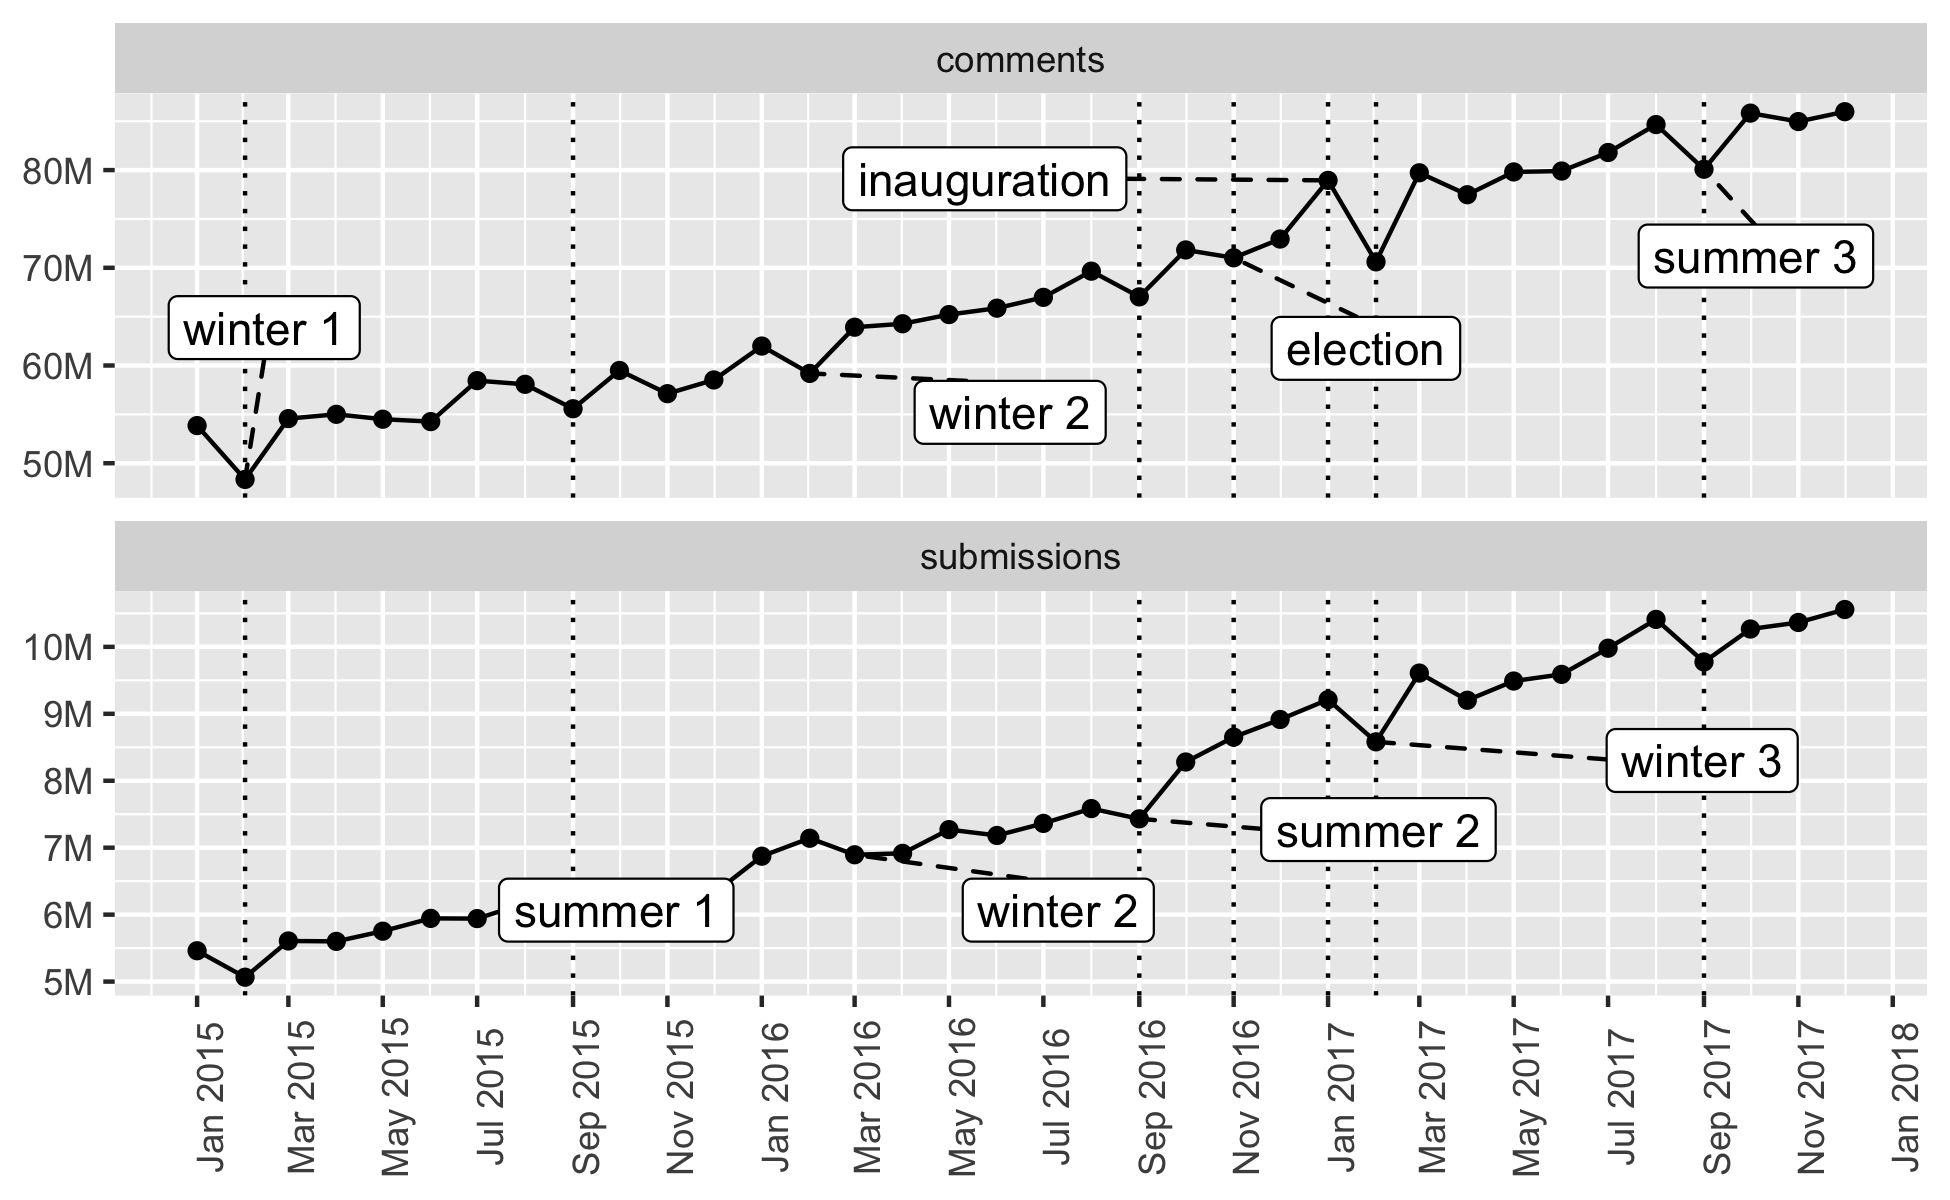
\includegraphics[width=\textwidth]{things}
\caption{Comments and submissions}
\end{figure}

The purpose of this chapter's analysis is to apply the existing literature and the framework from Chapter 2 to the 2016 presidential election in the United States.
Our base dataset contains all 2,715,684,936 items or 278,240,494 submissions and 2,437,444,442 comments by 26,777,565 users across 806,736 subreddits on Reddit from January 2015 to December 2017.
Comments and submissions posted to Reddit each month continue to increase linearly and change consistently with each other; the ratio of submissions to comments is never lower than 10.15\% or higher than 12.31\%.
In January 2015, there were 53,851,542 comments and 5,460,892 submissions, in December 2017, there were 85,973,810 comments and 10,557,874 submissions, increases of 59.65\% and 93.37\%.
Eternal September returns.
February 2017, the month after Trump's inauguration, brings decreases of -10.56\% for the comments and -6.85\% for the submissions, the biggest decrease in items month to month over the 3-year period.
 
\begin{figure}[!ht]
\centering
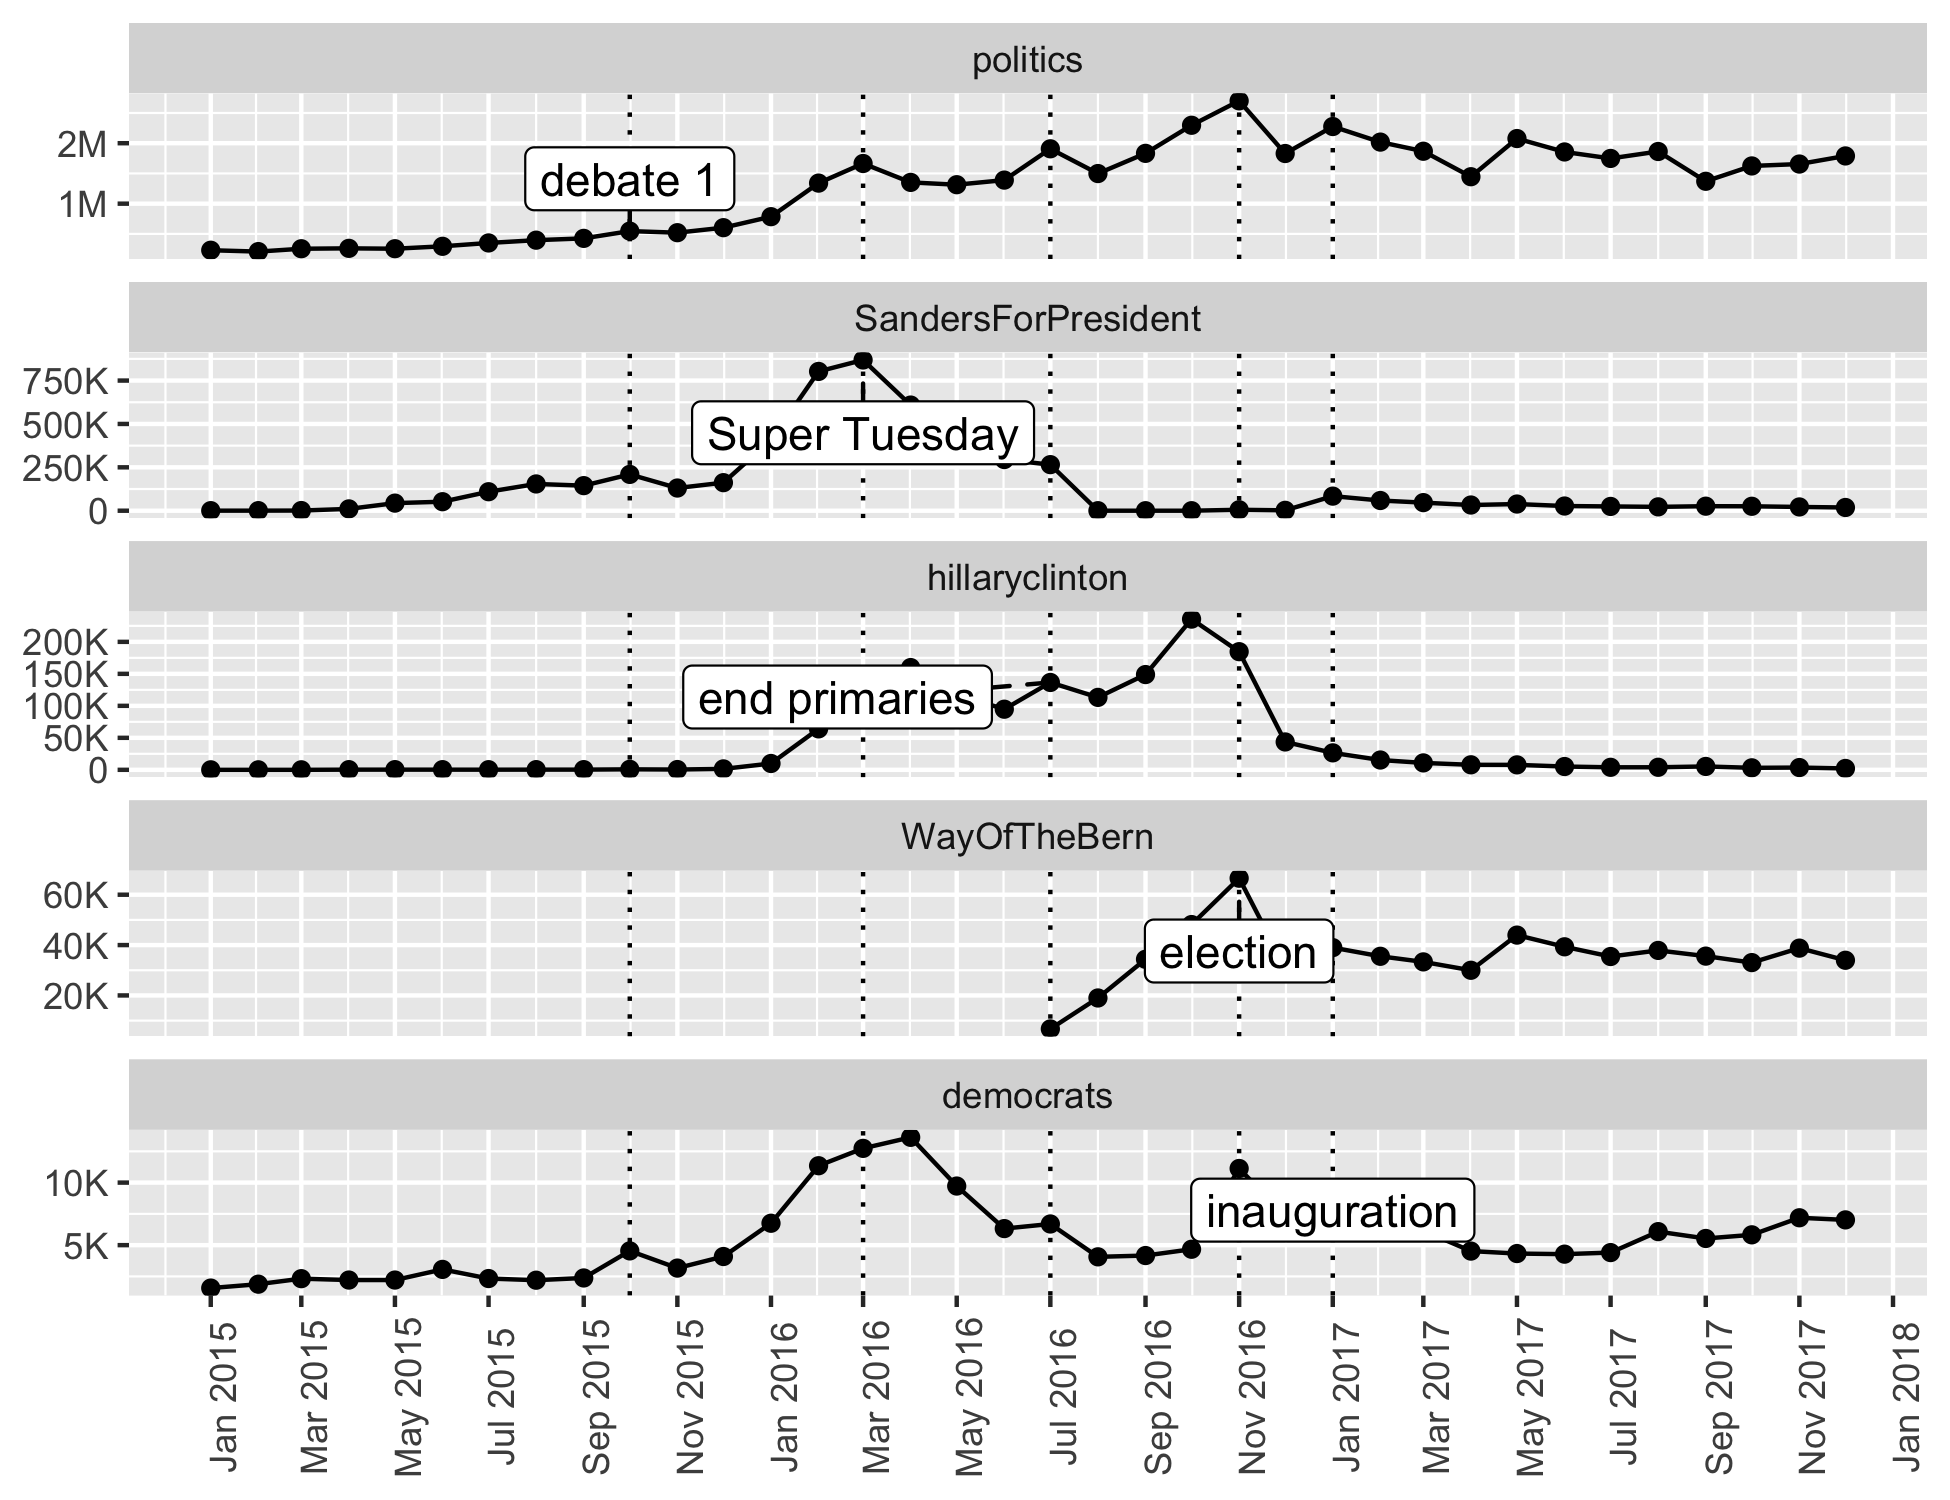
\includegraphics[width=\textwidth]{2016/progressive_count}
\caption{Comments and submissions (progressive subreddits)}
\label{fig:progressive_count}
\end{figure}

We identify ``progressive'' and ``conservative'' subsets of the data of popular political subreddits.
Figure \ref{fig:progressive_count} displays the progressive subreddits sorted by total number of items over the three-year period: r/politics (45,844,728 items), r/SandersForPresident (5,034,481), r/hillaryclinton (1,523,362), r/WayOfTheBern (641,654), and r/democrat (204,129).
The activity of these subreddits maps closely to the campaign cycle.
None of the subreddits register more than a small uptick in activity with the first debate in October 2015.
r/SandersForPresident peaks in March 2016 with 868,673 items before declining to 84,091 items in January 2017.
r/democrats has a delayed peak in April 2016 (13,630 items), then sees reduced interest until a rebound in November 2016 (11,130). 
r/WayOfTheBern also peaks in November (66,553 items) after opening in July with the Clinton nomination.
Both r/politics and r/hillaryclinton show increases, dips, then increases during the primary season (``U''), but the latter peaks in October (235,561) before sharply declining in January (26,528), while r/politics peaks in November (2,700,587) and maintains slightly reduced traffic after Trump's inauguration. 

\begin{figure}[!ht]
\centering
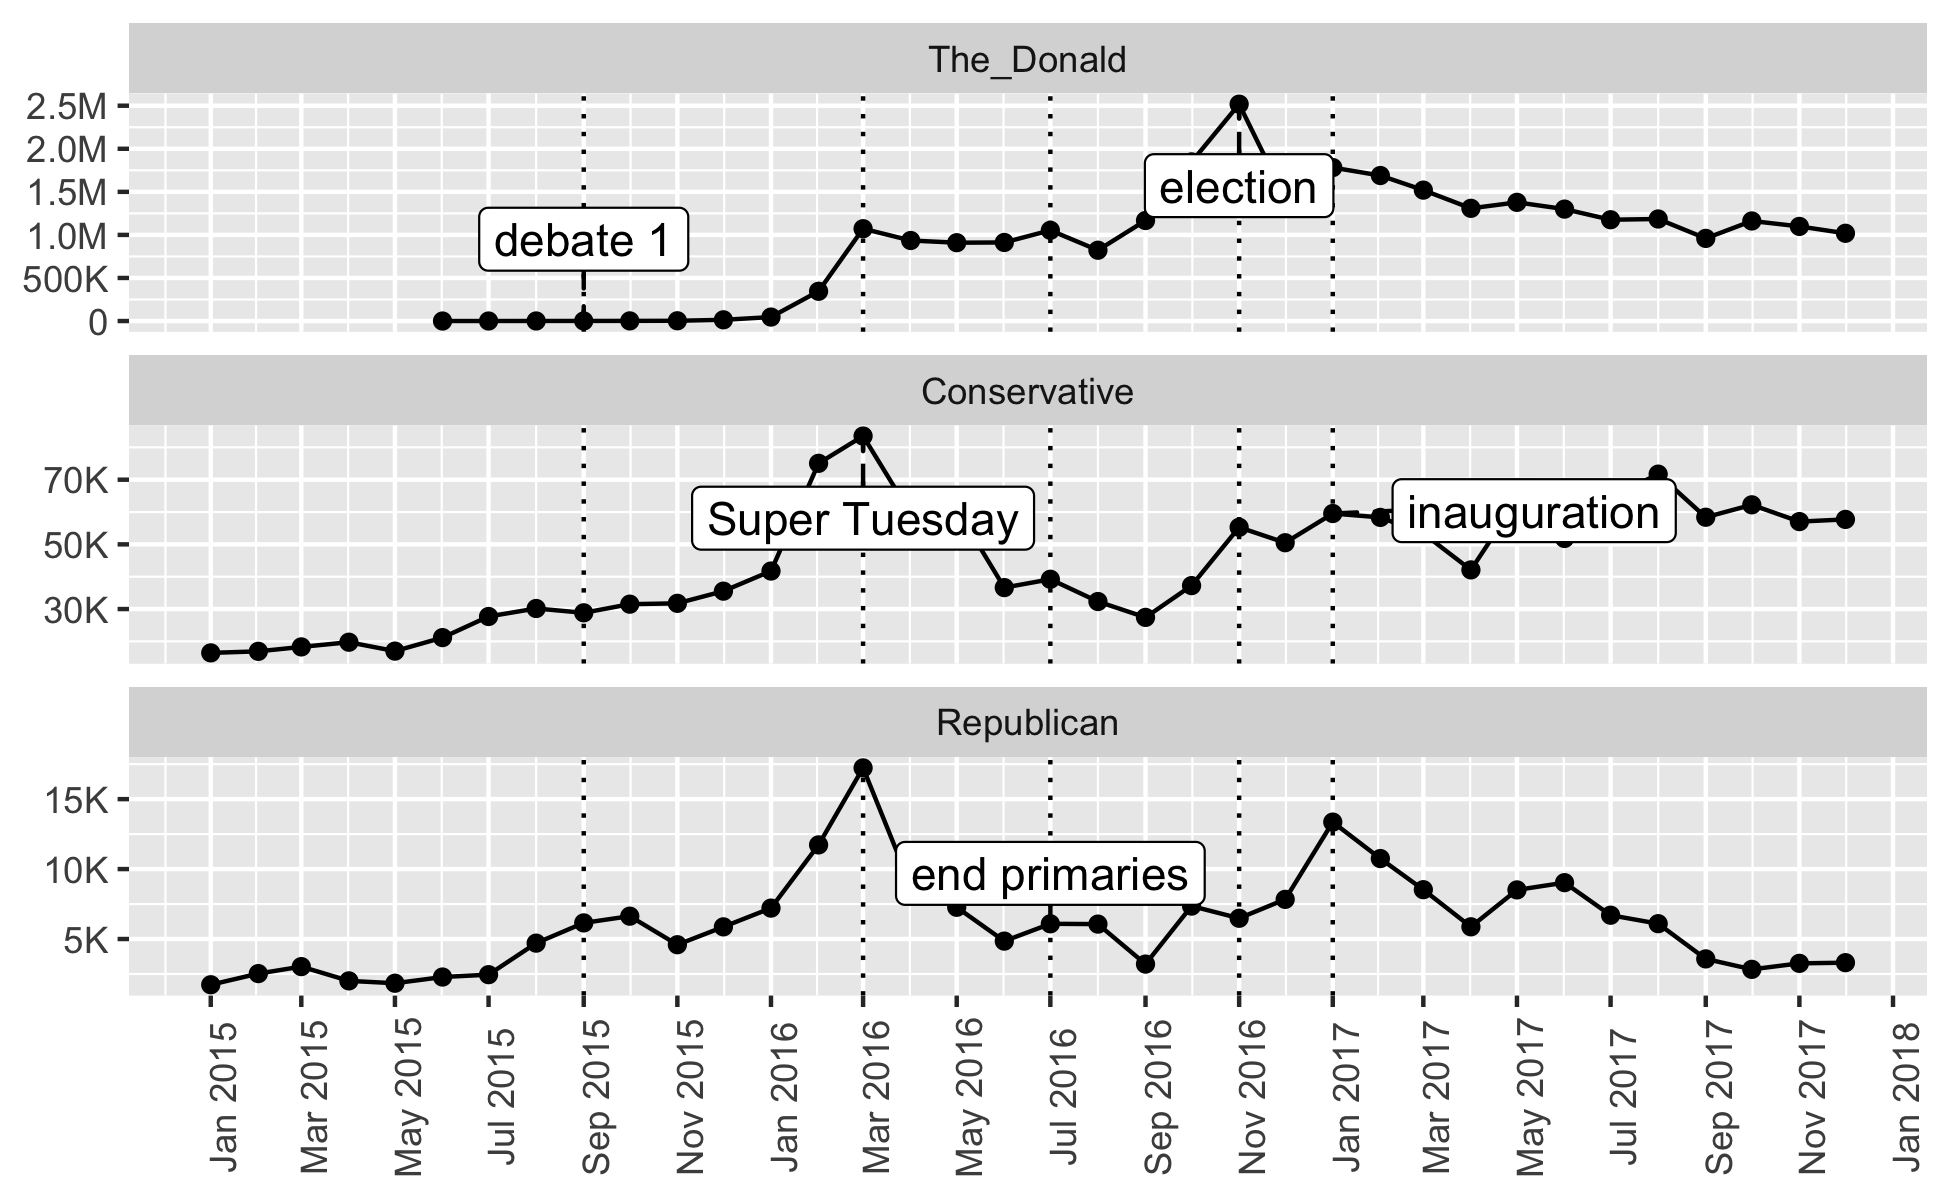
\includegraphics[width=\textwidth]{2016/conservative_count}
\caption{Comments and submissions (conservative subreddits)}
\label{fig:conservative_count}
\end{figure}

Figure \ref{fig:conservative_count} displays the conservative subreddits sorted by total number of items over the three-year period: r/The\_Donald (28,655,184 items), r/Conservative (1,595,012), and r/Republican (219,768).
Despite showing an awareness of and strategy including social media, the runner-up, Ted Cruz, does not have a large presence on Reddit.
Much like the progressive subreddits, these conservative subreddits track the campaign cycle and only see slight upticks in activity with the first debate.
r/Republican peaks in March 2016 (17,233), rebounds in January 2017 (13,358), then declines to levels seen before the election with 3,309 items in December 2017.
r/Conservative similarly peaks in March (83,501) and is more interested in the inauguration (59,540) than election (55,282), but maintains consistent traffic after November.
The activity on r/The\_Donald is representative of his candidacy.
In January 2016 there were only 46,003 items, increasing 2,230.37\% by March with 1,072,041 items, then following with the primary season trough (``U'') found in some of the progressive subreddits.
The subreddit peaks with 2,518,011 items in November 2016 and continues with high traffic through December 2017 (1,018,830).

\begin{figure}[!ht]
\centering
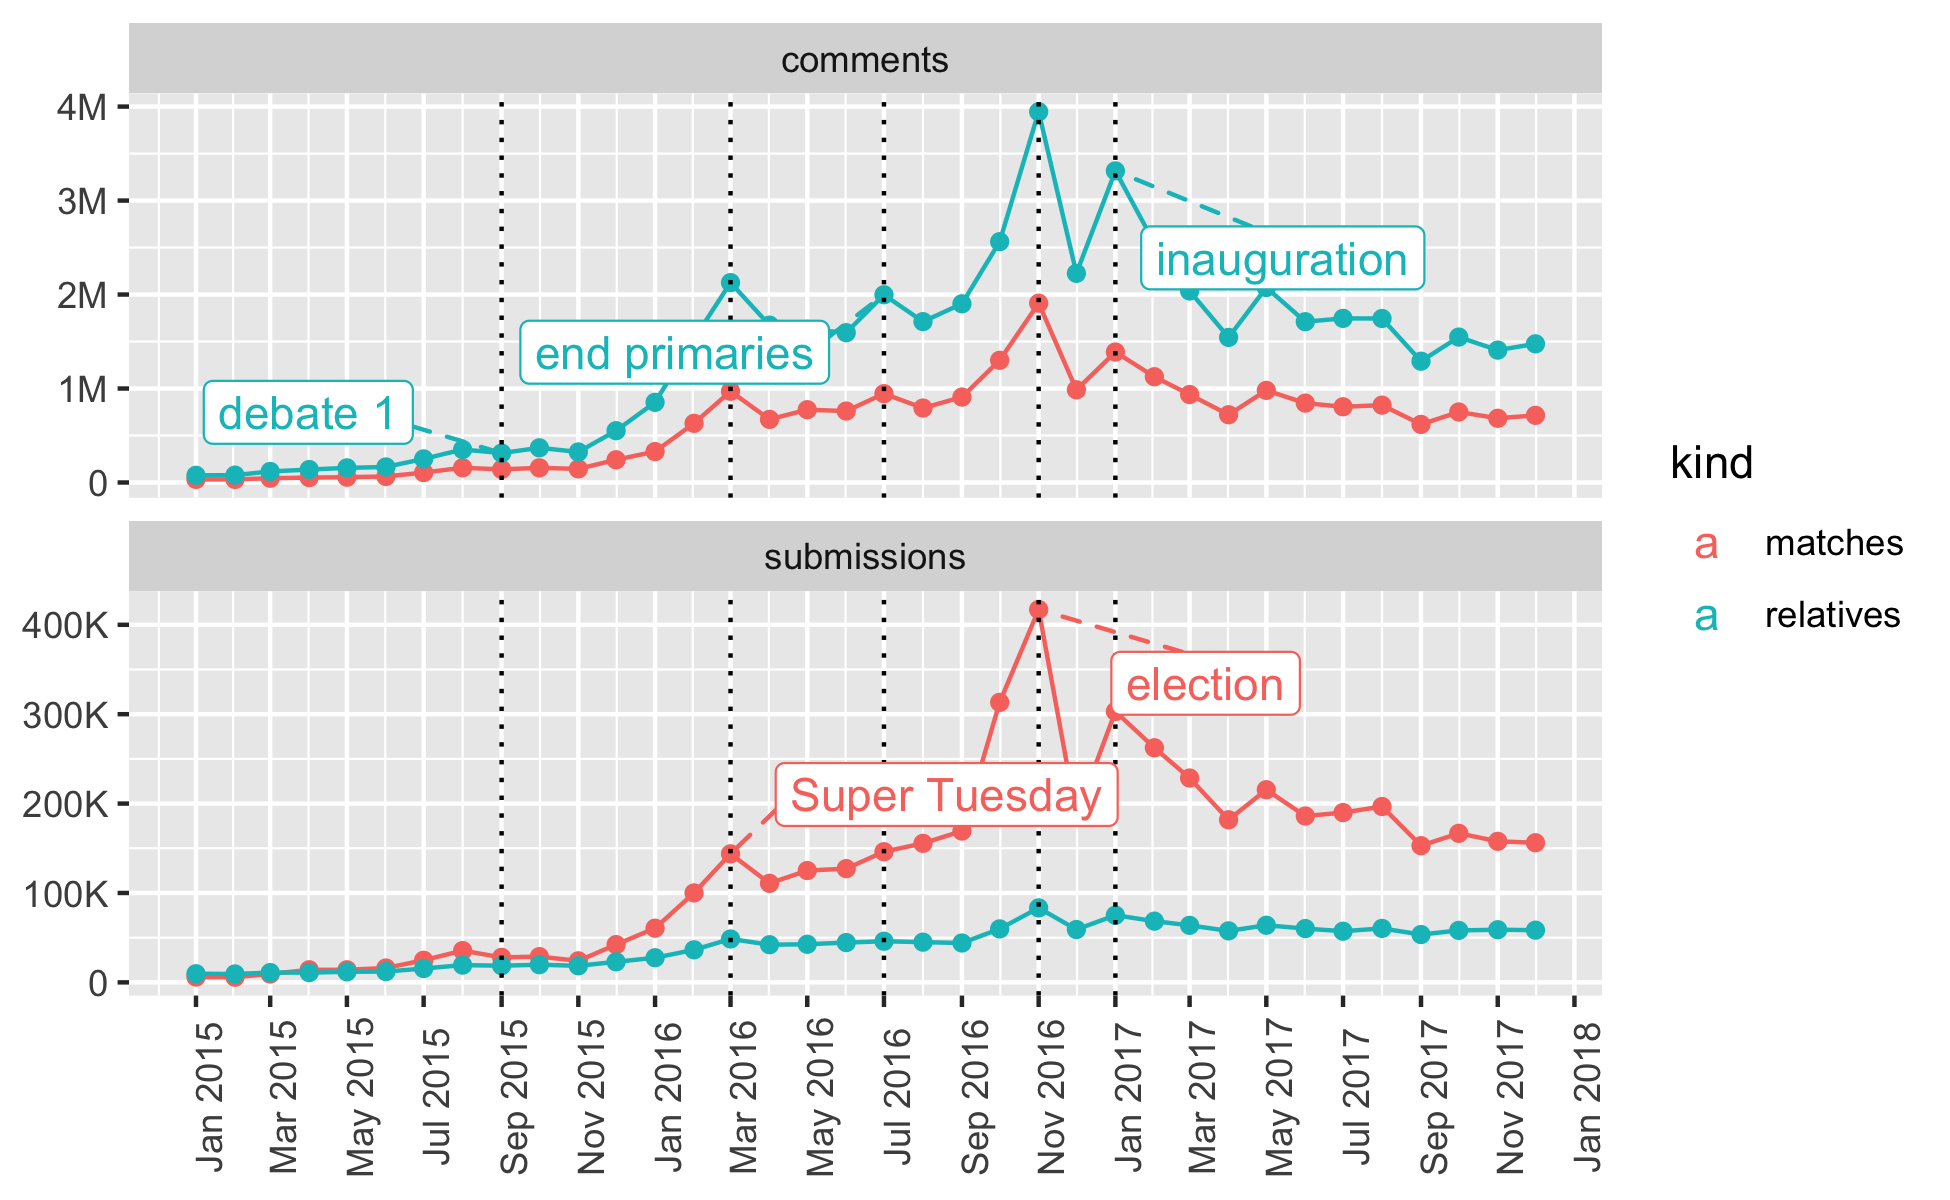
\includegraphics[width=\textwidth]{2016/match_count}
\caption{Comments and submissions}
\label{fig:match_count}
\end{figure}

Figure \ref{fig:match_count} displays matches and relatives by month.
The text component of each item (title and selftext for submissions, body for comments), is processed using spaCy, then filtered through a set of keywords and terms (case-insensitive).
The item is considered a ``match'' if ``Clinton'', ``Trump'', ``MAGA'', or terms related to ``caucus(ing)'' are present, or if various combinations of ``2016'', ``Democratic'', ``Republican'', ``Donald'', ``Hillary'', and terms related to ``debate(s)'', ``campaign(s)'', ``candidate(s)'', ``election(s)'', ``nominee(s)'', ``presidential'', ``primaries'', and ``vote(s)'' in the ``United States'' are found.
In addition to these ``matches'', items connected to them are marked as ``relatives''.
For submissions, this includes every comment in response to it, for comments, this includes the submission the comment is in response to as well as any comments (children) replying to the match and the replies to those replies, etc. 

Comments and submissions have very similar shapes and once again track the campaign cycle.
There is a very small uptick in activity with the first debates, a peak in March 2016, the familiar primary season U, absolute peak in November (1,907,800 matched, 1,242,938 related comments; 417,106 matched, 83,326 related submissions), rebound in January, and a final return to primary season levels.
In the immediate aftermath of the election, interest drops sharply, December 2016 bringing the greatest dip in matches month to month with -32.24\% fewer comments and -60.82\% fewer submissions.

\begin{figure}[!ht]
\centering
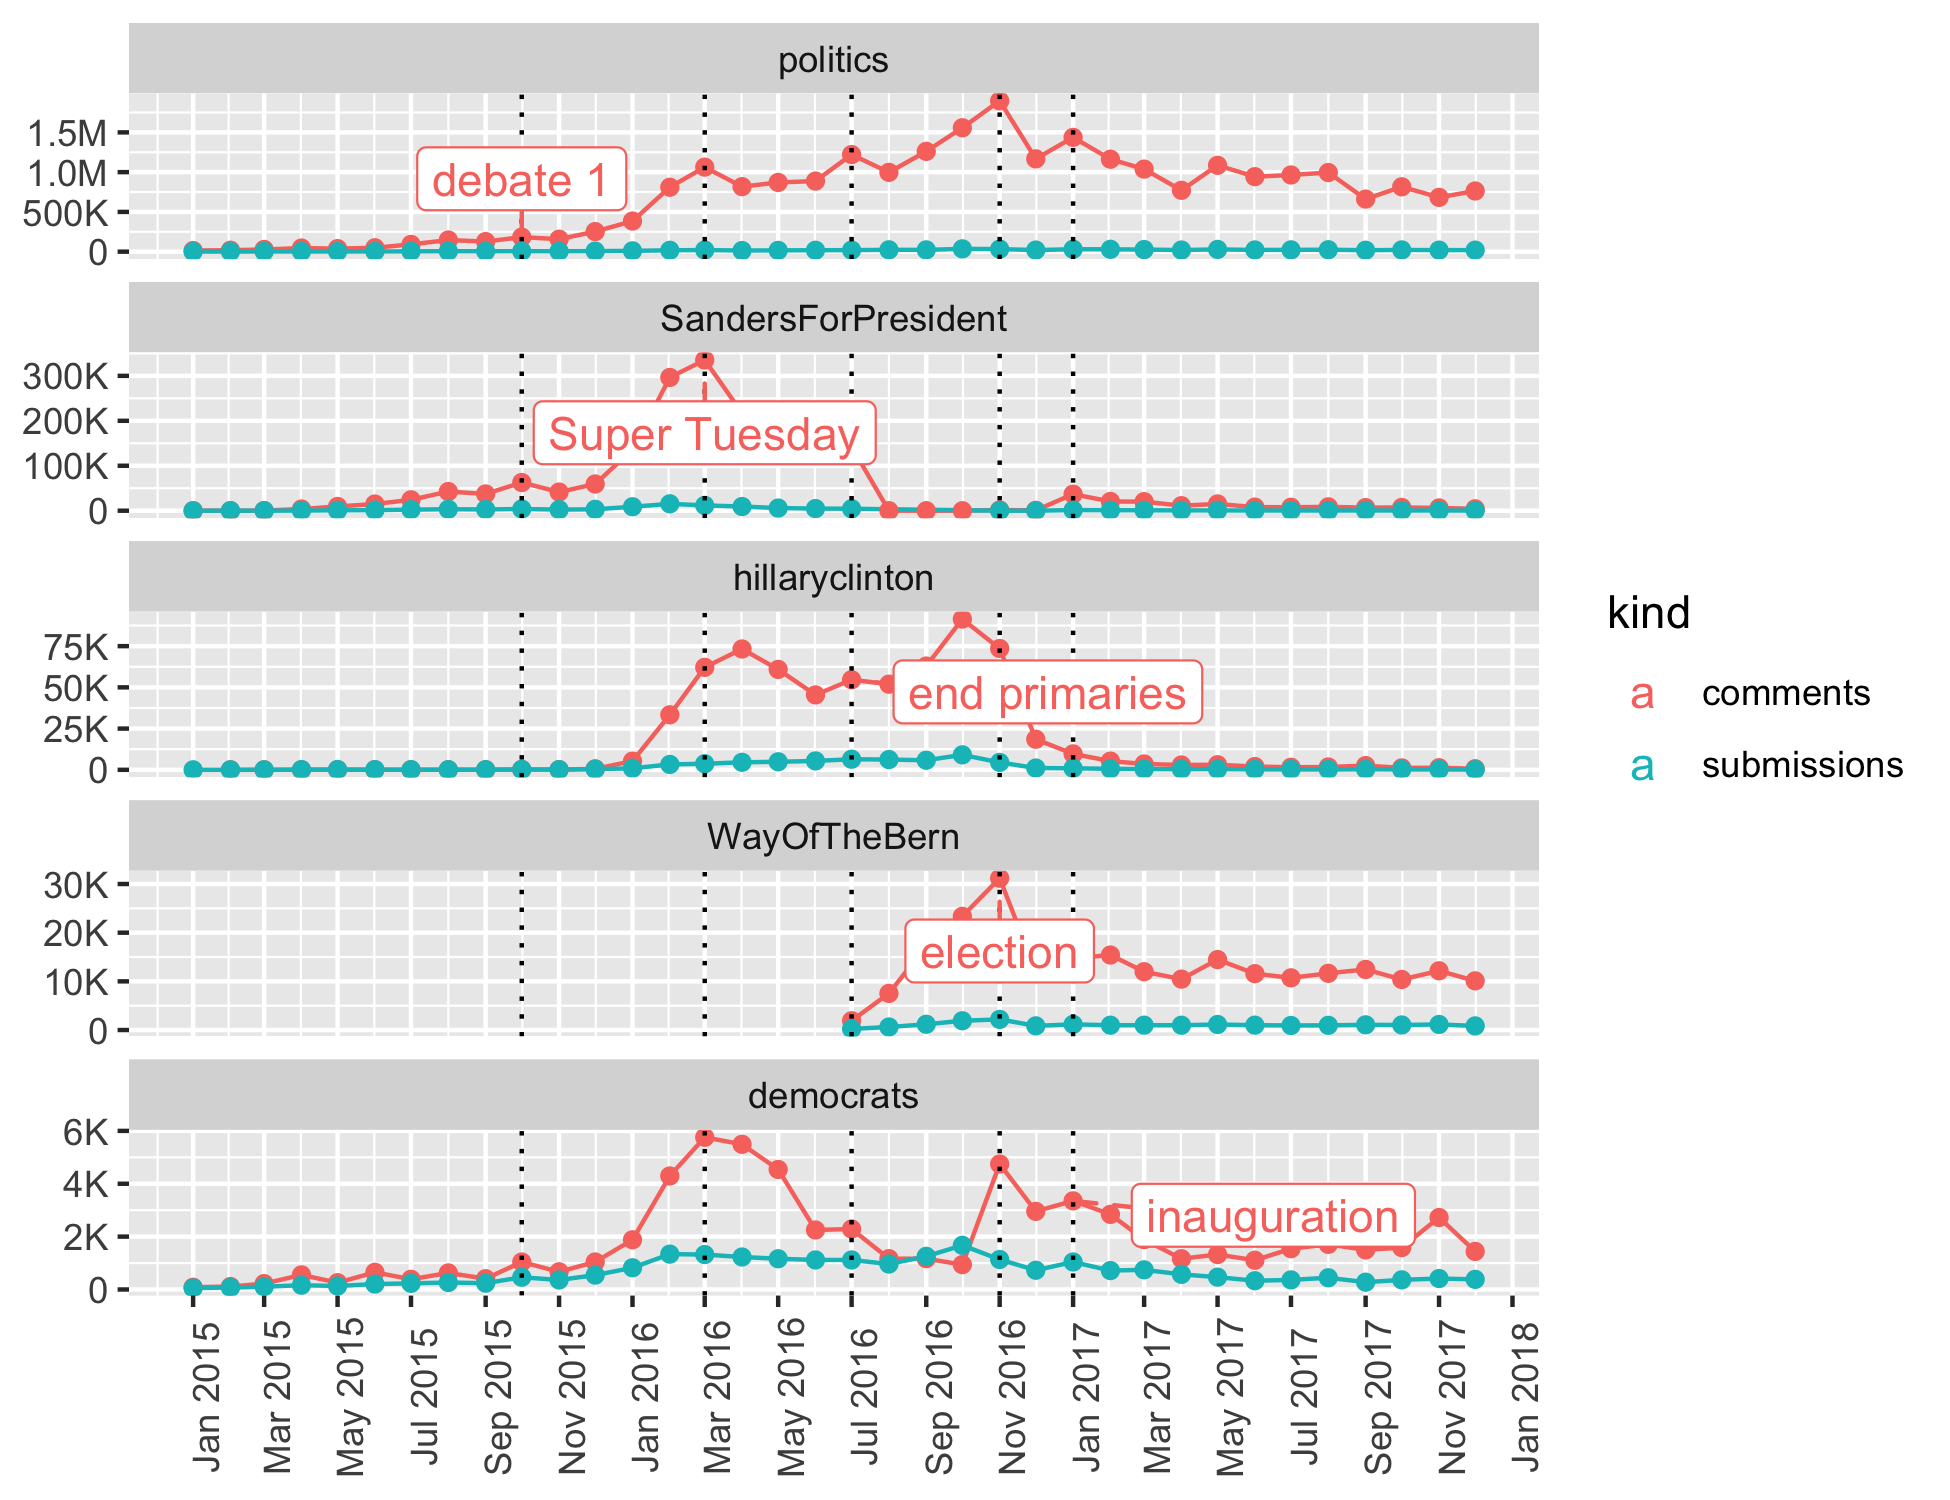
\includegraphics[width=\textwidth]{2016/progressive_match}
\caption{Matches and relatives (progressive subreddits)}
\label{fig:progressive_match}
\end{figure}

Figure \ref{fig:match_count} displays matches and relatives for submissions and comments in every subreddit combined.
However, it is likely that individual subreddits have different activity patterns.
To give another view of the data, Figure \ref{fig:progressive_match} displays graphs of the combined matches and relatives for submissions and comments for each progressive subreddit.
Using the same scale, it is more obvious that submissions are only a small percentage of activity, they are a prompt for discussion.
The content are the comments, unlike many news or social media sites.
The shape matches that of all comments and submissions in \ref{fig:progressive_count} until 2017 when they diverge more; the presidential election was the most dominant topic, a large fraction of political discussion throughout 2016.
r/politics (1,896,280,350 comment, 32,311 submission matches and relatives) and r/WayOfTheBern (31,192, 2,188 matches and relatives) peak in November 2016, r/SandersForPresident (335,343, 11,790) and r/democrats (5,756, 1,321) in March, and r/hillaryclinton (91,397, 9,087) had the most activity in October prior to the election. 

\begin{figure}[!ht]
\centering
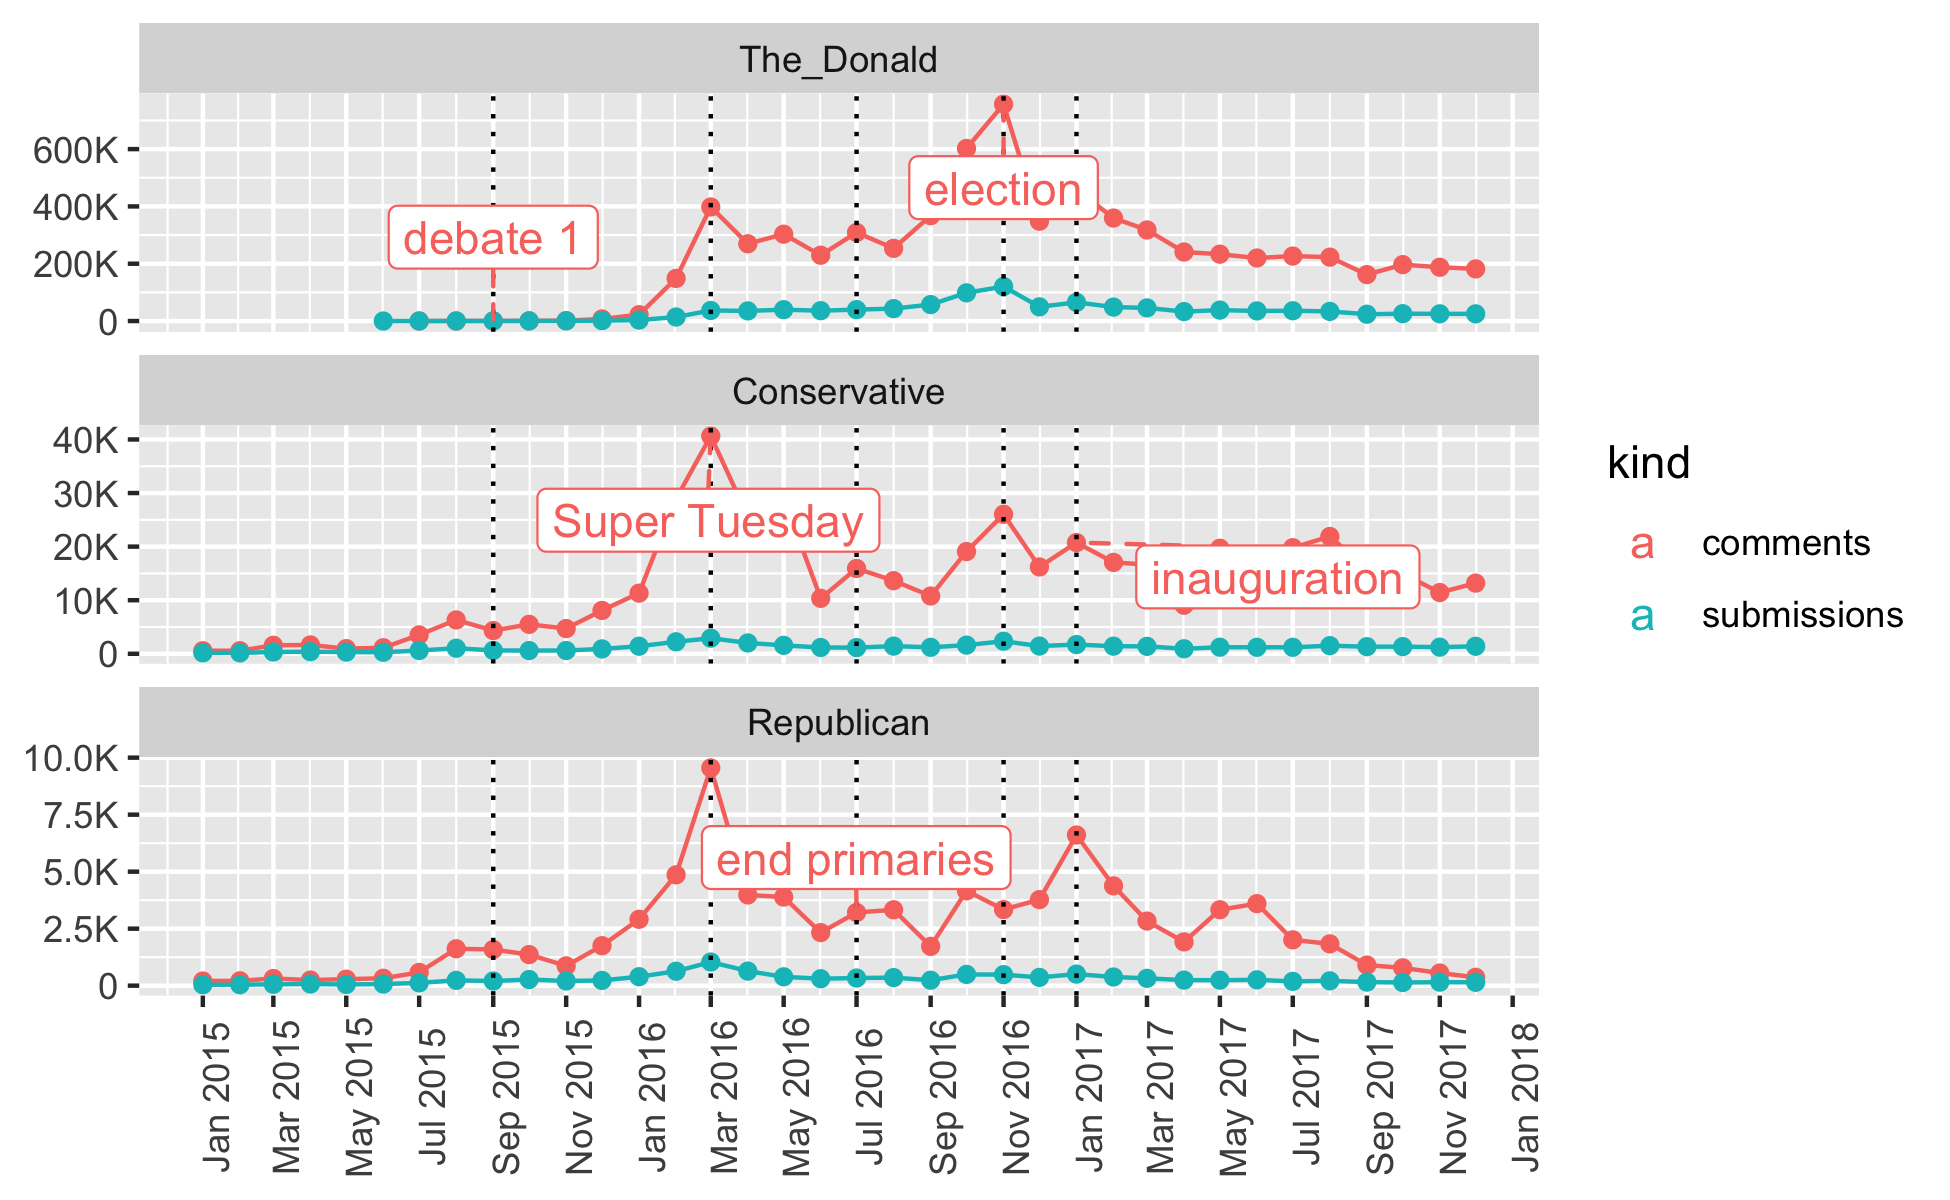
\includegraphics[width=\textwidth]{2016/conservative_match}
\caption{Matches and relatives (conservative subreddits)}
\label{fig:conservative_match}
\end{figure}

Figure \ref{fig:conservative_match} displays graphs of the combined matches and relatives for submissions and comments for each conservative subreddit.
Here too submissions are a small fraction of comments, and the shape is similar to that of all items in \ref{fig:conservative_count}.
r/Conservative (40,640 comment, 2,909 submission matches and relatives) and r/Republican (9,551, 1,037 matches and relatives) peak in March 2016, the former shows more interest in the inauguration than the election.
Unsurprisingly, r/The\_Donald peaks in November with 756,835 comment, 120,485 submission matches and relatives.
In comparison, there are more submission matches that month than the entire 95,739 matches and relatives in r/Republican from 2015-2017.

\begin{table}[!ht]
\centering
\caption{Subreddits}
\begin{tabular}{lrrrrr}
\toprule
subreddit & \% & matches* & items & match \% & users \\
\midrule
worldnews             &   26.42 &   8643307 &    11747329 &    73.58 &   670840 \\
ukraine               &   10.39 &   3398449 &     4449535 &    76.38 &   226133 \\
UkrainianConflict     &    4.60 &   1504119 &     1765260 &    85.21 &   111672 \\
UkraineWarVideoReport &    3.46 &   1133154 &     1554034 &    72.92 &   125078 \\
CombatFootage         &    3.08 &   1007114 &     1543356 &    65.25 &   105349 \\
europe                &    2.22 &    725743 &     1857161 &    39.08 &    65027 \\
interestingasfuck     &    2.16 &    706541 &     4724053 &    14.96 &   218316 \\ß
news                  &    1.50 &    490912 &     5105814 &     9.61 &   102269 \\
politics              &    1.49 &    488251 &     6034055 &     8.09 &   111127 \\
AskARussian           &    1.46 &    476317 &      645065 &    73.84 &    25777 \\
conspiracy            &    1.40 &    458934 &     4302073 &    10.67 &    49986 \\
PublicFreakout        &    1.14 &    371466 &     5078293 &     7.31 &   106408 \\
neoliberal            &    1.09 &    355758 &     2846818 &    12.50 &    12885 \\
Damnthatsinteresting  &    1.06 &    348223 &     3066770 &    11.35 &   137484 \\
RussiaUkraineWar2022  &    0.82 &    269498 &      353670 &    76.20 &    35129 \\
ukpolitics            &    0.78 &    253829 &     1164034 &    21.81 &    10976 \\
NonCredibleDefense    &    0.69 &    226047 &      903671 &    25.01 &    21413 \\
nextfuckinglevel      &    0.65 &    211148 &     2937907 &     7.19 &    93475 \\
de                    &    0.62 &    201494 &     1500742 &    13.43 &    11344 \\
CryptoCurrency        &    0.55 &    181134 &     4980486 &     3.64 &    30981 \\
AskReddit             &    0.55 &    179205 &    39669986 &     0.45 &    56466 \\
ThatsInsane           &    0.51 &    168041 &     1069685 &    15.71 &    69375 \\
wallstreetbets        &    0.51 &    167041 &     7255226 &     2.30 &    46690 \\
Conservative          &    0.42 &    137499 &     1615715 &     8.51 &    19408 \\
CredibleDefense       &    0.34 &    112541 &      127050 &    88.58 &     6494 \\
russia                &    0.33 &    109417 &      171355 &    63.85 &    11906 \\
MapPorn               &    0.28 &     93019 &     1058404 &     8.79 &    32329 \\
canada                &    0.27 &     88474 &     1916732 &     4.62 &    16165 \\
CrazyFuckingVideos    &    0.26 &     85168 &     1691437 &     5.04 &    35943 \\
UkraineInvasionVideos &    0.26 &     84348 &      115132 &    73.26 &    13433 \\
summary (top 30)      &   69.32 &  22676191 &   121250848 &    32.64 &          \\
summary (all)         &  100.00 &  32713731 &  1456280549 &     0.49 &  2565090 \\
\bottomrule
\end{tabular}

\label{tab:subreddits}
\end{table}

Table \ref{tab:subreddits} displays the 30 subreddits with the most combined matches and relatives.
There are 75,322,866 matches and relatives by 2,672,292 unique users across 70,783 subreddits (with 70 excluded).
These 30 subreddits contain 73.8\% of all matches and relatives and these items are matched an average 24.45\% of the time, compared to the 0.78\% match rate average of all subreddits.
Our selected political subreddits that are present have higher, though not the highest, match rates: r/politics (56.67\%), r/The\_Donald (28.06\%), r/SandersForPresident (38.84\%), r/hillaryclinton (48.04\%), r/Conservative (32.80\%), and r/WayOfTheBern (40.31\%).
Several other subreddits (r/EnoughTrumpSpam), might be useful to add to the partisan groupings but there is much more data available than the previous chapter, and significant traffic comes after the election.
r/politics and r/The\_Donald are more than 43.68\% of all matches and relatives, and we note the presence of r/conspiracy, the 8th most-active subreddit with its 18.84\% match rate. 
Finally, r/politics has more than 3 times as many combined matches as r/The\_Donald, which has more than 4 times as many matches as r/SandersForPresident, which has more than 10 times as many matches as r/hillaryclinton.
These Trump and Sanders subreddits have the large majority of their activity after 2015.

\subsection{Classification}

\begin{table}[!ht]
\centering
\caption{Cites (matched and related items)}
\begin{tabular}{lrrrrrr}
\toprule
{} & \% & cites & users &  cites / & \% prog & \% cons \\
domain &  &  &  & users & users & users \\
\midrule
reddit.com*           &   21.94 &   2722645 &   630963 &         4.32 &         13.41 &          9.79 \\
youtube.com*          &    9.62 &   1193237 &   251651 &         4.74 &         16.49 &         17.00 \\
imgur.com             &    6.01 &    746031 &   200126 &         3.73 &         10.76 &          9.57 \\
wikipedia.org         &    3.70 &    459470 &   126526 &         3.63 &         19.83 &         11.21 \\
twitter.com*          &    3.45 &    428391 &    81020 &         5.29 &         23.65 &         22.73 \\
washingtonpost.com    &    2.03 &    252175 &    68845 &         3.66 &         40.00 &         19.00 \\
nytimes.com*          &    1.37 &    170305 &    54124 &         3.15 &         32.52 &         16.96 \\
cnn.com               &    1.13 &    139847 &    47536 &         2.94 &         36.94 &         22.44 \\
archive.org*          &    1.06 &    131008 &    20095 &         6.52 &         29.30 &         37.80 \\
google.com*           &    1.05 &    130314 &    48537 &         2.68 &         16.23 &          9.06 \\
politico.com          &    0.97 &    120307 &    37074 &         3.25 &         45.09 &         26.10 \\
thehill.com           &    0.90 &    111112 &    30702 &         3.62 &         43.44 &         28.39 \\
theguardian.com       &    0.84 &    103685 &    39020 &         2.66 &         41.09 &         17.61 \\
huffingtonpost.com*   &    0.72 &     89205 &    32861 &         2.71 &         44.03 &         18.67 \\
sli.mg                &    0.72 &     88865 &    15886 &         5.59 &         10.85 &         22.45 \\
independent.co.uk     &    0.62 &     77328 &    22716 &         3.40 &         44.67 &         13.21 \\
reuters.com           &    0.56 &     69324 &    23100 &         3.00 &         36.07 &         23.85 \\
wikileaks.org         &    0.52 &     64918 &    12213 &         5.32 &         19.71 &         23.63 \\
breitbart.com         &    0.50 &     62530 &    17220 &         3.63 &         25.17 &         52.35 \\
politifact.com        &    0.49 &     60982 &    26742 &         2.28 &         32.46 &         13.41 \\
foxnews.com           &    0.46 &     57092 &    23051 &         2.48 &         24.60 &         35.29 \\
bbc.com*              &    0.43 &     53800 &    24014 &         2.24 &         22.17 &         17.11 \\
businessinsider.com   &    0.41 &     51133 &    24106 &         2.12 &         34.92 &         21.58 \\
fivethirtyeight.com   &    0.38 &     47223 &    18570 &         2.54 &         39.89 &         11.51 \\
facebook.com*         &    0.37 &     46391 &    18790 &         2.47 &         18.70 &         10.88 \\
nbcnews.com           &    0.37 &     46260 &    19792 &         2.34 &         42.94 &         20.70 \\
realclearpolitics.com &    0.34 &     42197 &    15416 &         2.74 &         34.86 &         20.09 \\
theatlantic.com       &    0.34 &     41577 &    19370 &         2.15 &         44.51 &         17.66 \\
go.com                &    0.33 &     41301 &    17435 &         2.37 &         44.54 &         17.30 \\
npr.org               &    0.31 &     38915 &    18260 &         2.13 &         43.26 &         13.57 \\
summary (top 30)      &   61.96 &   7687568 &          &         3.32 &         31.07 &         20.03 \\
summary (all)         &  100.00 &  11761790 &  1174637 &         1.97 &         45.13 &         41.51 \\
\bottomrule
\end{tabular}

\label{tab:doms_2016}
\end{table}

We filter out 61 apparent bots (helper and otherwise) and 9 domains, as well as combine link shorteners and domain aliases.
Table \ref{tab:doms_2016} displays the 30 most-cited domains within the matched and related items.
There are in total 11,761,790 cites by 1,174,637 unique users; these 30 domains are 61.96\% of these cites.
While reddit.com, youtube.com, imgur.com, wikipedia.org, and twitter.com are 44.72\% of cites, of the remaining sites only washingtonpost.com is over 2\%; this large set of domains is varied and widely-distributed.
Reddit domains are the most-cited: 2,722,645 times by 630,963 users, wikileaks.org has the fewest users (12,312) out of the top 30 with 64,918 cites.
It is one of four domains of 30 with more than 5 cites per user, the average of 3.32 and overall average of 1.97 cites per user suggest that bot activity is uncommon.
Using selected domains described in the following, users are categorized as ``progressive'' or ``conservative'' based on whether they have cited those domains at least 25 times over the 3-year period.
The splits of users sharing different domains is as expected: washingtonpost.com (40\% of cites by progressives, 19\% by conservatives), huffingtonpost.com (44.04, 18.67), breitbart.com (25.17, 52.35), foxnews.com (24.6, 35.29), npr.org (43.26, 13.57).
Partisan averages are higher for the overall list than the top 30 because neutral users share these more common sites and niche domains dominate the tails.

\begin{table}[!ht]
\centering
\caption{Cites (progressive subreddits)}
\begin{tabular}{lrrrrr}
\toprule
domain & \% & cites & users & cites/users & \% prog users \\
\midrule
reddit.com*           &   10.13 &   291044 &   46989 &         6.19 &         37.34 \\
youtube.com*          &    9.22 &   264895 &   71275 &         3.72 &         25.49 \\
wikipedia.org         &    4.85 &   139381 &   42928 &         3.25 &         29.76 \\
washingtonpost.com    &    4.02 &   115514 &   31883 &         3.62 &         40.80 \\
twitter.com*          &    3.43 &    98469 &   25088 &         3.92 &         40.90 \\
imgur.com             &    3.17 &    91103 &   33552 &         2.72 &         23.75 \\
nytimes.com*          &    2.33 &    66843 &   24029 &         2.78 &         34.76 \\
politico.com          &    2.04 &    58680 &   18706 &         3.14 &         45.24 \\
cnn.com               &    2.02 &    57984 &   21799 &         2.66 &         31.63 \\
thehill.com           &    1.87 &    53660 &   14906 &         3.60 &         42.35 \\
huffingtonpost.com*   &    1.48 &    42635 &   15816 &         2.70 &         43.57 \\
google.com*           &    1.14 &    32674 &   14949 &         2.19 &         23.72 \\
theguardian.com       &    1.02 &    29356 &   12838 &         2.29 &         42.95 \\
politifact.com        &    1.02 &    29191 &   12472 &         2.34 &         39.37 \\
fivethirtyeight.com   &    0.85 &    24443 &    9816 &         2.49 &         44.00 \\
realclearpolitics.com &    0.77 &    22083 &    8266 &         2.67 &         39.00 \\
businessinsider.com   &    0.70 &    20244 &    9612 &         2.11 &         39.33 \\
reuters.com           &    0.68 &    19480 &    8195 &         2.38 &         37.38 \\
nbcnews.com           &    0.64 &    18374 &    8850 &         2.08 &         40.61 \\
foxnews.com           &    0.61 &    17631 &    8816 &         2.00 &         24.80 \\
theatlantic.com       &    0.58 &    16561 &    8160 &         2.03 &         48.35 \\
go.com                &    0.54 &    15527 &    7866 &         1.97 &         37.79 \\
independent.co.uk     &    0.53 &    15208 &    6743 &         2.26 &         35.31 \\
thedailybeast.com     &    0.53 &    15196 &    6391 &         2.38 &         47.99 \\
wikileaks.org         &    0.51 &    14760 &    3752 &         3.93 &         23.32 \\
usatoday.com          &    0.51 &    14739 &    7834 &         1.88 &         36.46 \\
bloomberg.com         &    0.51 &    14525 &    6849 &         2.12 &         45.44 \\
npr.org               &    0.49 &    14149 &    7800 &         1.81 &         38.28 \\
vox.com               &    0.48 &    13823 &    5807 &         2.38 &         50.50 \\
slate.com             &    0.46 &    13250 &    6451 &         2.05 &         49.86 \\
summary (top 30)      &   57.14 &  1641422 &         &         2.72 &         38.00 \\
summary (all)         &  100.00 &  2811462 &  244521 &         1.34 &         60.58 \\
\bottomrule
\end{tabular}

\label{tab:doms_progressive}
\end{table}

Table \ref{tab:doms_progressive} displays the 30 most-cited domains within the five selected progressive subreddits.
There are 2,811,462 cites by 244,521 unique users; the top 30 domains are 57.14\% of all cites in these subreddits.
These domains appear similar to the previous table of all domains:
sharing-oriented domains (youtube.com) are the most common, the set of domains  is nearly the same, and the cites per user averages of 2.72 and 1.34 are representative and suggest natural user activity.
The average of 38\% of progressive users posting these domains also captures the makeup of these subreddits. 

\begin{table}[!ht]
\centering
\caption{Cites (conservative subreddits)}
\begin{tabular}{lrrrrr}
\toprule
domain &       \% &    cites &   users &  cites/users &  \% cons users \\
\midrule
reddit.com*            &   26.35 &   495851 &   79256 &         6.26 &         15.57 \\
youtube.com*           &   13.81 &   259777 &   42047 &         6.18 &         27.74 \\
imgur.com              &    8.85 &   166463 &   25814 &         6.45 &         10.21 \\
twitter.com*           &    5.09 &    95753 &   14465 &         6.62 &         40.20 \\
sli.mg                 &    3.79 &    71300 &   12121 &         5.88 &         21.35 \\
archive.org*           &    3.02 &    56805 &    7470 &         7.60 &         34.73 \\
breitbart.com          &    1.49 &    28037 &    5453 &         5.14 &         63.87 \\
wikipedia.org          &    1.44 &    27117 &   10062 &         2.69 &         30.72 \\
wikileaks.org          &    1.19 &    22462 &    3882 &         5.79 &         29.24 \\
donaldjtrump.com       &    1.08 &    20362 &    2633 &         7.73 &         49.49 \\
google.com*            &    1.00 &    18893 &    4695 &         4.02 &         14.89 \\
foxnews.com            &    0.81 &    15159 &    5139 &         2.95 &         49.17 \\
magaimg.net            &    0.71 &    13278 &    2158 &         6.15 &         62.05 \\
infowars.com           &    0.59 &    11187 &    4803 &         2.33 &         34.63 \\
thegatewaypundit.com   &    0.54 &    10232 &    1549 &         6.61 &         73.70 \\
thehill.com            &    0.54 &    10224 &    3529 &         2.90 &         53.87 \\
washingtonpost.com     &    0.50 &     9437 &    4404 &         2.14 &         32.93 \\
dailycaller.com        &    0.49 &     9239 &    2440 &         3.79 &         65.57 \\
votinginfoproject.org  &    0.47 &     8855 &       2 &     4,427.50 &          0.07 \\
nytimes.com*           &    0.47 &     8752 &    4545 &         1.93 &         31.33 \\
politico.com           &    0.45 &     8444 &    3411 &         2.48 &         49.79 \\
facebook.com*          &    0.43 &     8100 &    3508 &         2.31 &         23.05 \\
cnn.com                &    0.43 &     8090 &    4072 &         1.99 &         27.22 \\
dailymail.co.uk        &    0.42 &     7968 &    3268 &         2.44 &         43.76 \\
washingtontimes.com    &    0.32 &     6095 &    2118 &         2.88 &         62.95 \\
washingtonexaminer.com &    0.31 &     5906 &    1846 &         3.20 &         64.60 \\
realclearpolitics.com  &    0.29 &     5512 &    1981 &         2.78 &         41.60 \\
whitehouse.gov         &    0.28 &     5257 &    1287 &         4.08 &         64.75 \\
zerohedge.com          &    0.26 &     4965 &    1731 &         2.87 &         55.03 \\
stopthesteal.org       &    0.26 &     4837 &      50 &        96.74 &          0.62 \\
summary (top 30)       &   75.70 &  1424357 &         &       154.75 &         39.16 \\
summary (all)          &  100.00 &  1835490 &  145149 &         2.03 &         60.62 \\
\bottomrule
\end{tabular}

\label{tab:doms_conservative}
\end{table}

Table \ref{tab:doms_conservative} displays the top 30 most-cited domains within the three selected conservative subreddits.
There are 1,835,490 cites by 145,149 unique users; they comprise 75.7\% of all cites in these subreddits.
Compared to the progressives, similar domains are present and dominate the very top, but also present are a number of much more partisan domains including infowars.com and dailycaller.com.
These partisan domains have much higher percentages of citations by conservative users: magaimg.net (62.05\%) and washingtontimes.com (52.95\%) are representative, the average is only pulled down because of the presence of broader domains like twitter.com.
The overall cites per user average are only 2.03, which does not suggest bot activity.
votinginfoproject.org, shared by only two users, is the most obvious example of a general election resource common across Reddit, but note the presence of the more targeted stopthesteal.org, shared 4,837 times by 50 users.

\begin{table}[!ht]
\centering
\caption{Selected progressive domains}
\begin{tabular}{llrrrrr}
\toprule
rank & domain & \% & cites & users & cites/users & \% prog users \\
\midrule
11               &    huffingtonpost.com* &   11.61 &   42635 &   15816 &         2.70 &         43.57 \\
13               &        theguardian.com &    7.99 &   29356 &   12838 &         2.29 &         42.95 \\
15               &    fivethirtyeight.com &    6.66 &   24443 &    9816 &         2.49 &         44.00 \\
21               &        theatlantic.com &    4.51 &   16561 &    8160 &         2.03 &         48.35 \\
28               &                npr.org &    3.85 &   14149 &    7800 &         1.81 &         38.28 \\
29               &                vox.com &    3.76 &   13823 &    5807 &         2.38 &         50.50 \\
30               &              slate.com &    3.61 &   13250 &    6451 &         2.05 &         49.86 \\
33               &              salon.com &    3.33 &   12231 &    5055 &         2.42 &         49.88 \\
35               &      berniesanders.com &    3.28 &   12039 &    3880 &         3.10 &         57.57 \\
36               &              msnbc.com &    3.22 &   11828 &    5283 &         2.24 &         48.27 \\
43               &           dailykos.com &    2.79 &   10243 &    4955 &         2.07 &         47.76 \\
46               &        motherjones.com &    2.69 &    9867 &    4763 &         2.07 &         52.89 \\
49               &     hillaryclinton.com &    2.56 &    9412 &    3657 &         2.57 &         53.91 \\
50               &      thinkprogress.org &    2.44 &    8948 &    3864 &         2.32 &         57.15 \\
51               &           buzzfeed.com &    2.40 &    8796 &    3954 &         2.22 &         48.01 \\
54               &  talkingpointsmemo.com &    2.33 &    8548 &    3048 &         2.80 &         59.27 \\
59               &              nymag.com &    2.01 &    7368 &    3458 &         2.13 &         54.86 \\
62               &          newyorker.com &    1.81 &    6665 &    3647 &         1.83 &         45.09 \\
66               &           mediaite.com &    1.55 &    5684 &    2882 &         1.97 &         44.23 \\
72               &       theintercept.com &    1.40 &    5149 &    2544 &         2.02 &         47.95 \\
76               &               vice.com &    1.33 &    4896 &    2789 &         1.76 &         44.36 \\
77               &          thenation.com &    1.33 &    4877 &    2570 &         1.90 &         56.02 \\
78               &           rawstory.com &    1.33 &    4874 &    1892 &         2.58 &         41.55 \\
84               &         vanityfair.com &    1.21 &    4446 &    2557 &         1.74 &         45.86 \\
91               &       mediamatters.org &    1.08 &    3969 &    1986 &         2.00 &         51.35 \\
92               &       commondreams.org &    1.06 &    3883 &    1411 &         2.75 &         61.47 \\
94               &           alternet.org &    1.02 &    3748 &    2027 &         1.85 &         47.76 \\
96               &        feelthebern.org &    1.00 &    3688 &    1384 &         2.66 &         55.15 \\
97               &        newrepublic.com &    0.96 &    3540 &    1704 &         2.08 &         57.82 \\
98               &       rollingstone.com &    0.96 &    3517 &    2112 &         1.67 &         45.64 \\
& summary (top 30) & 85.08 &  312433 &         &         2.22 &         49.71 \\
& summary (all)    & 100.00 &  367244 &  66584 &         5.52 &         47.25 \\
\bottomrule
\end{tabular}

\label{tab:doms_progressive1}
\end{table}

To get the final set of progressive users, 66 domains were selected from the progressive subreddits.
Table \ref{tab:doms_progressive1} displays the 30 most-cited within matched and related items, ranked by their placement in Table \ref{tab:doms_progressive}.
There are 367,244 cites by 66,584 unique users; the top 30 are 85.08\% of cites.
This variety of progressive sources on average is cited by progressive users (those with at least 25 cites of these domains) 47.25\% of the time.

\begin{table}[!ht]
\centering
\caption{Selected conservative domains}
\begin{tabular}{llrrrrr}
\toprule
 & & & & & cites / & \% cons \\
rank & domain & \% & cites & users & users & users \\
\midrule
7                &                 breitbart.com &   15.12 &   28037 &    5453 &         5.14 &         63.87 \\
10               &              donaldjtrump.com &   10.98 &   20362 &    2633 &         7.73 &         49.49 \\
12               &                   foxnews.com &    8.17 &   15159 &    5139 &         2.95 &         49.17 \\
13               &                   magaimg.net &    7.16 &   13278 &    2158 &         6.15 &         62.05 \\
14               &                  infowars.com &    6.03 &   11187 &    4803 &         2.33 &         34.63 \\
15               &          thegatewaypundit.com &    5.52 &   10232 &    1549 &         6.61 &         73.70 \\
18               &               dailycaller.com &    4.98 &    9239 &    2440 &         3.79 &         65.57 \\
25               &           washingtontimes.com &    3.29 &    6095 &    2118 &         2.88 &         62.95 \\
26               &        washingtonexaminer.com &    3.18 &    5906 &    1846 &         3.20 &         64.60 \\
29               &                 zerohedge.com &    2.68 &    4965 &    1731 &         2.87 &         55.03 \\
30               &              stopthesteal.org &    2.61 &    4837 &      50 &        96.74 &          0.62 \\
33               &                    nypost.com &    2.17 &    4026 &    1596 &         2.52 &         57.25 \\
35               &                 dailywire.com &    1.91 &    3540 &    1136 &         3.12 &         58.64 \\
39               &                  townhall.com &    1.74 &    3230 &     989 &         3.27 &         70.96 \\
43               &            nationalreview.com &    1.45 &    2688 &    1043 &         2.58 &         54.65 \\
47               &  theconservativetreehouse.com &    1.40 &    2592 &     764 &         3.39 &         60.61 \\
50               &                       wnd.com &    1.28 &    2381 &     969 &         2.46 &         59.09 \\
51               &                  redstate.com &    1.23 &    2290 &     644 &         3.56 &         72.75 \\
53               &                   newsmax.com &    1.20 &    2222 &     759 &         2.93 &         63.46 \\
55               &                        rt.com &    1.19 &    2215 &    1035 &         2.14 &         50.34 \\
56               &                freebeacon.com &    1.18 &    2191 &     887 &         2.47 &         66.23 \\
64               &               telegraph.co.uk &    0.93 &    1720 &    1126 &         1.53 &         34.88 \\
66               &           americanthinker.com &    0.90 &    1675 &     563 &         2.98 &         67.70 \\
71               &                    hotair.com &    0.82 &    1512 &     453 &         3.34 &         71.83 \\
70               &                   dilbert.com &    0.82 &    1512 &     805 &         1.88 &         34.46 \\
79               &                 express.co.uk &    0.70 &    1301 &     615 &         2.12 &         58.03 \\
81               &                  theblaze.com &    0.68 &    1258 &     581 &         2.17 &         49.68 \\
82               &                   pjmedia.com &    0.68 &    1256 &     425 &         2.96 &         71.26 \\
88               &             judicialwatch.org &    0.64 &    1181 &     514 &         2.30 &         62.32 \\
91               &             thefederalist.com &    0.62 &    1147 &     526 &         2.18 &         66.70 \\
& summary (top 30) & 91.26 &  169234 &         &         6.34 &         57.08 \\
& summary (all)    & 100.00 &  185443 &  23728 &         7.82 &         51.06 \\
\bottomrule
\end{tabular}

\label{tab:doms_conservative1}
\end{table}

To get the final set of conservative users, 61 domains were selected from the conservative subreddits.
Table \ref{tab:doms_conservative1} displays the 30 most-cited within matched and related items, ranked by their placement in Table \ref{tab:doms_conservative}.
There are 185,443 cites by 23,728 unique users; the top 30 are 91.26\% of cites.
We note the presence of commonly-cited niche and partisan sources.
infowars.com, owned by conspiracy entrepreneur Alex Jones, is the 14th most-cited domain in conservative subreddits.
stopthesteal.org, while only cited by 50 users, is the 30th most-cited conservative domain.
rt.com is ranked 55th; personality-driven outlets including Ben Shapiro at dailywire.com and Glenn Beck's theblaze.com are also present.
These conservative sites are cited by conservative users 51.06\% of the time.

\begin{table}[!ht]
\centering
\footnotesize
\caption{Wiki articles (progressive subreddits)}
\begin{tabular}{lrrrrr}
\toprule
{} & \% & cites & users & cites / & \% prog \\
wikipedia.com/wiki/ & & & & users & users \\
\midrule
Whataboutism                                  &    0.63 &     883 &    587 &         1.50 &         26.84 \\
Southern\_Strategy                             &    0.51 &     704 &    448 &         1.57 &         42.47 \\
Foundations\_Of\_Geopolitics                    &    0.50 &     692 &    403 &         1.72 &         18.06 \\
Bush\_White\_House\_Email\_Controversy            &    0.49 &     687 &    396 &         1.73 &         46.14 \\
Democratic\_Party\_Presidential\_Primaries,\_2016 &    0.41 &     566 &    417 &         1.36 &         38.16 \\
National\_Popular\_Vote\_Interstate\_Compact      &    0.39 &     544 &    346 &         1.57 &         29.23 \\
Democratic\_Party\_Presidential\_Primaries,\_2008 &    0.31 &     439 &    355 &         1.24 &         34.85 \\
Clinton\_Health\_Care\_Plan\_Of\_1993              &    0.28 &     391 &    318 &         1.23 &         36.57 \\
United\_States\_Presidential\_Election,\_2016     &    0.27 &     383 &    309 &         1.24 &         30.29 \\
Bill\_Clinton\_Sexual\_Misconduct\_Allegations    &    0.26 &     364 &    299 &         1.22 &         18.96 \\
List\_Of\_Democratic\_Party\_Superdelegates,\_2016 &    0.26 &     359 &    282 &         1.27 &         28.69 \\
Dunning\%E2\%80\%93Kruger\_Effect                 &    0.25 &     345 &    267 &         1.29 &         27.83 \\
Citizens\_United\_V.\_Fec                        &    0.22 &     311 &    236 &         1.32 &         43.73 \\
Saturday\_Night\_Massacre                       &    0.22 &     307 &    268 &         1.15 &         29.32 \\
Fairness\_Doctrine                             &    0.21 &     289 &    249 &         1.16 &         27.68 \\
James\_O\%27Keefe                               &    0.21 &     287 &    133 &         2.16 &         47.39 \\
United\_States\_Presidential\_Line\_Of\_Succession &    0.21 &     287 &    262 &         1.10 &         17.77 \\
Flag\_Protection\_Act\_Of\_2005                   &    0.21 &     286 &    175 &         1.63 &         20.28 \\
Poe\%27S\_Law                                   &    0.20 &     275 &    243 &         1.13 &         22.18 \\
Narcissistic\_Personality\_Disorder             &    0.20 &     272 &    125 &         2.18 &         49.26 \\
Neoliberalism                                 &    0.19 &     270 &    195 &         1.38 &         31.11 \\
Logan\_Act                                     &    0.19 &     268 &    228 &         1.18 &         20.52 \\
Fascism                                       &    0.19 &     259 &    190 &         1.36 &         21.24 \\
Duverger\%27S\_Law                              &    0.19 &     259 &    174 &         1.49 &         37.45 \\
Hillary\_Clinton                               &    0.18 &     255 &    202 &         1.26 &         34.12 \\
Iraq\_Resolution                               &    0.18 &     253 &    193 &         1.31 &         47.83 \\
Psychological\_Projection                      &    0.18 &     250 &    191 &         1.31 &         31.20 \\
United\_States\_Presidential\_Election,\_2012     &    0.17 &     241 &    212 &         1.14 &         28.63 \\
Ad\_Hominem                                    &    0.17 &     237 &    194 &         1.22 &         30.38 \\
Hillary\_Clinton\_Email\_Controversy             &    0.17 &     237 &    179 &         1.32 &         26.16 \\
summary (top 30)                              &    8.04 &   11200 &        &         1.39 &         31.48 \\
summary (all)                                 &  100.00 &  109772 &  42932 &         1.15 &         65.14 \\
\bottomrule
\end{tabular}

\label{tab:doms_progressive_wiki}
\end{table}

Finally, Table \ref{tab:doms_progressive_wiki} displays the 30 most-cited Wikipedia articles in the progressive subreddits.
There are 109,772 citations by 42,932 users; the top 30 are only 8.04\% of cites.
Generally, these articles are relevant to the 2016 campaign and most of are not strongly favored by progressive users.
The exceptions seem to be rebuttals to partisan attacks, such as the Bush email controversy, with 46.14\% cites by progressives.
The Foundations of Geopolitics is a supposedly influential work among Russian nationalists; while it may have limited relevance here, it became prominent in 2022 with Russia's invasion of Ukraine, to be covered next chapter.

\begin{table}[!ht]
\centering
\footnotesize
\caption{Wiki articles (conservative subreddits)}
\begin{tabular}{lrrrrr}
\toprule
{} & \% & cites & users & cites / & \% cons \\
wikipedia.com/wiki/ & & & & users & users \\
\midrule
Moveon.Org                                         &    1.43 &    388 &     38 &        10.21 &         94.07 \\
Media\_Matters\_For\_America                          &    1.40 &    380 &     34 &        11.18 &         95.00 \\
New\_Life\_Children\%27S\_Refuge\_Case                  &    0.31 &     85 &     25 &         3.40 &         71.76 \\
Republican\_Party\_Presidential\_Primaries,\_2016      &    0.31 &     84 &     54 &         1.56 &         45.24 \\
Fifth\_Column                                       &    0.29 &     79 &     18 &         4.39 &         49.37 \\
Operation\_Mockingbird                              &    0.29 &     79 &     55 &         1.44 &         17.72 \\
United\_States\_Presidential\_Election,\_2016          &    0.26 &     71 &     54 &         1.31 &         21.13 \\
Alveda\_King                                        &    0.26 &     71 &      2 &        35.50 &        100.00 \\
Bill\_Clinton\_Pardon\_Controversy                    &    0.26 &     70 &     42 &         1.67 &         47.14 \\
Marc\_Rich                                          &    0.25 &     69 &     40 &         1.73 &         46.38 \\
Donald\_Trump                                       &    0.24 &     64 &     47 &         1.36 &         31.25 \\
Psychological\_Projection                           &    0.21 &     57 &     43 &         1.33 &         35.09 \\
Faithless\_Elector                                  &    0.20 &     54 &     41 &         1.32 &         11.11 \\
Bill\_Clinton\_Sexual\_Misconduct\_Allegations         &    0.18 &     49 &     44 &         1.11 &         22.45 \\
Qatar-Turkey\_Pipeline                              &    0.18 &     49 &     20 &         2.45 &          8.16 \\
Moloch                                             &    0.18 &     48 &     16 &         3.00 &         66.67 \\
List\_Of\_Islamist\_Terrorist\_Attacks                 &    0.17 &     45 &     27 &         1.67 &         26.67 \\
Frankfurt\_School                                   &    0.16 &     44 &     13 &         3.38 &         75.00 \\
Overton\_Window                                     &    0.16 &     44 &     39 &         1.13 &         27.27 \\
List\_Of\_Donald\_Trump\_Presidential\_Campaign\_Endo... &    0.16 &     43 &     24 &         1.79 &         41.86 \\
Atf\_Gunwalking\_Scandal                             &    0.15 &     41 &     23 &         1.78 &         63.41 \\
Telecommunications\_Act\_Of\_1996                     &    0.15 &     40 &     36 &         1.11 &         12.50 \\
Flag\_Protection\_Act\_Of\_2005                        &    0.15 &     40 &     37 &         1.08 &         25.00 \\
Inbreeding\_Depression                              &    0.14 &     39 &      3 &        13.00 &         94.87 \\
John\_Podesta                                       &    0.14 &     39 &     25 &         1.56 &         46.15 \\
Bohemian\_Grove                                     &    0.14 &     37 &      7 &         5.29 &         86.49 \\
Robert\_Byrd                                        &    0.14 &     37 &     31 &         1.19 &          8.11 \\
Secure\_Fence\_Act\_Of\_2006                           &    0.14 &     37 &     31 &         1.19 &         35.14 \\
Operation\_Northwoods                               &    0.13 &     36 &     26 &         1.38 &         22.22 \\
Little\_Saint\_James,\_U.S.\_Virgin\_Islands            &    0.13 &     36 &      6 &         6.00 &         91.67 \\
summary (top 30)                                   &    8.32 &   2255 &        &         4.15 &         47.30 \\
summary (all)                                      &  100.00 &  14859 &  10062 &         1.30 &         76.89 \\
\bottomrule
\end{tabular}

\label{tab:doms_conservative_wiki}
\end{table}

In the conservative subreddits there are 14,859 citations of Wikipedia by 10,062 users; the top 30 make up 8.32\% of all cites
There are relatively few cites overall, only 2 articles have more than 100, and multiple articles have fewer than 10 users.
Within this limited sample size is a focus on conspiracies.
Operation Mockingbird and Operation Northwoods were operations by intelligence agencies in the 1960s aimed at the public,
Bohemian Grove has long been a hot topic in conspiracy circles.
Bill Clinton is an issue in both progressive and conservative subreddits.
There does seem to be an attempt to connect those around the Clintons with rumors of various forms of abuse, material associated with ``Pizzagate'' and an attack on Comet Ping Pong, a pizzeria, in Washington, D.C.

\begin{table}[!ht]
\centering
\caption{User groups}
\begin{tabular}{lrrrrrr}
\hline
& & & comment & comment & submission & submission \\
group & users & doms & matches & relatives & matches & relatives \\
\hline
neutral &  193647 &  346457 &           381264 &             776965 &               39312 &                 52842 \\
spreader &     262 &   80023 &            40618 &              52658 &               19011 &                  7143 \\
superspreader &      75 &   43239 &            13201 &              16223 &               13280 &                  3118 \\
totals &  193910 &  518141 &           459054 &            1033697 &               87008 &                 72688 \\
\hline
\end{tabular}

\label{tab:2016_groups}
\end{table}

Wikipedia articles are not used to categorize users.
Table \ref{tab:2016_groups} displays basic stats about these groups: the number of users within, how many domains they post, and the quantity of matches and relatives for both submissions and comments.
Of the 2,530,782 users in the matched data, 2,437 (0.1\%) are ``conservative'' with at least 25 cites of our selected conservative domains, 4,375 (0.17\%)  are ``progressive'' with at least 25 cites of the selected progressive domains.
The totals include bots and subreddits are not excluded.
Once again, the filtered users are a very small part of the dataset.

Unlike the previous chapter, we use a higher single threshold of 25 cites because while these different sources have measurable ideologies, there is no simple government-owned or similar heuristic.
Users categorized as ``rus'' posted certain domains, those that were neutral did not.
With a much larger dataset, it is not uncommon for users to post both progressive and conservative domains; out of 5,928 users in the progressive and conservative groups, 884 have at least 25 cites of each.
We attempt to get around this by not including newspapers of record like The New York Times and Washington Post in either domain set, but in partisan contexts users will often post sources they disagree with to mock them.
Therefore, we create two more groups of users, ``progressive+'' and ``conservative+'', where users in each group have cited one set of domains at least 100 times more than the other.
Using this measure, there are 527 progressive+ users and 260 conservative+ users.

\subsection{Network Analysis}

\begin{figure}[!ht]
\centering
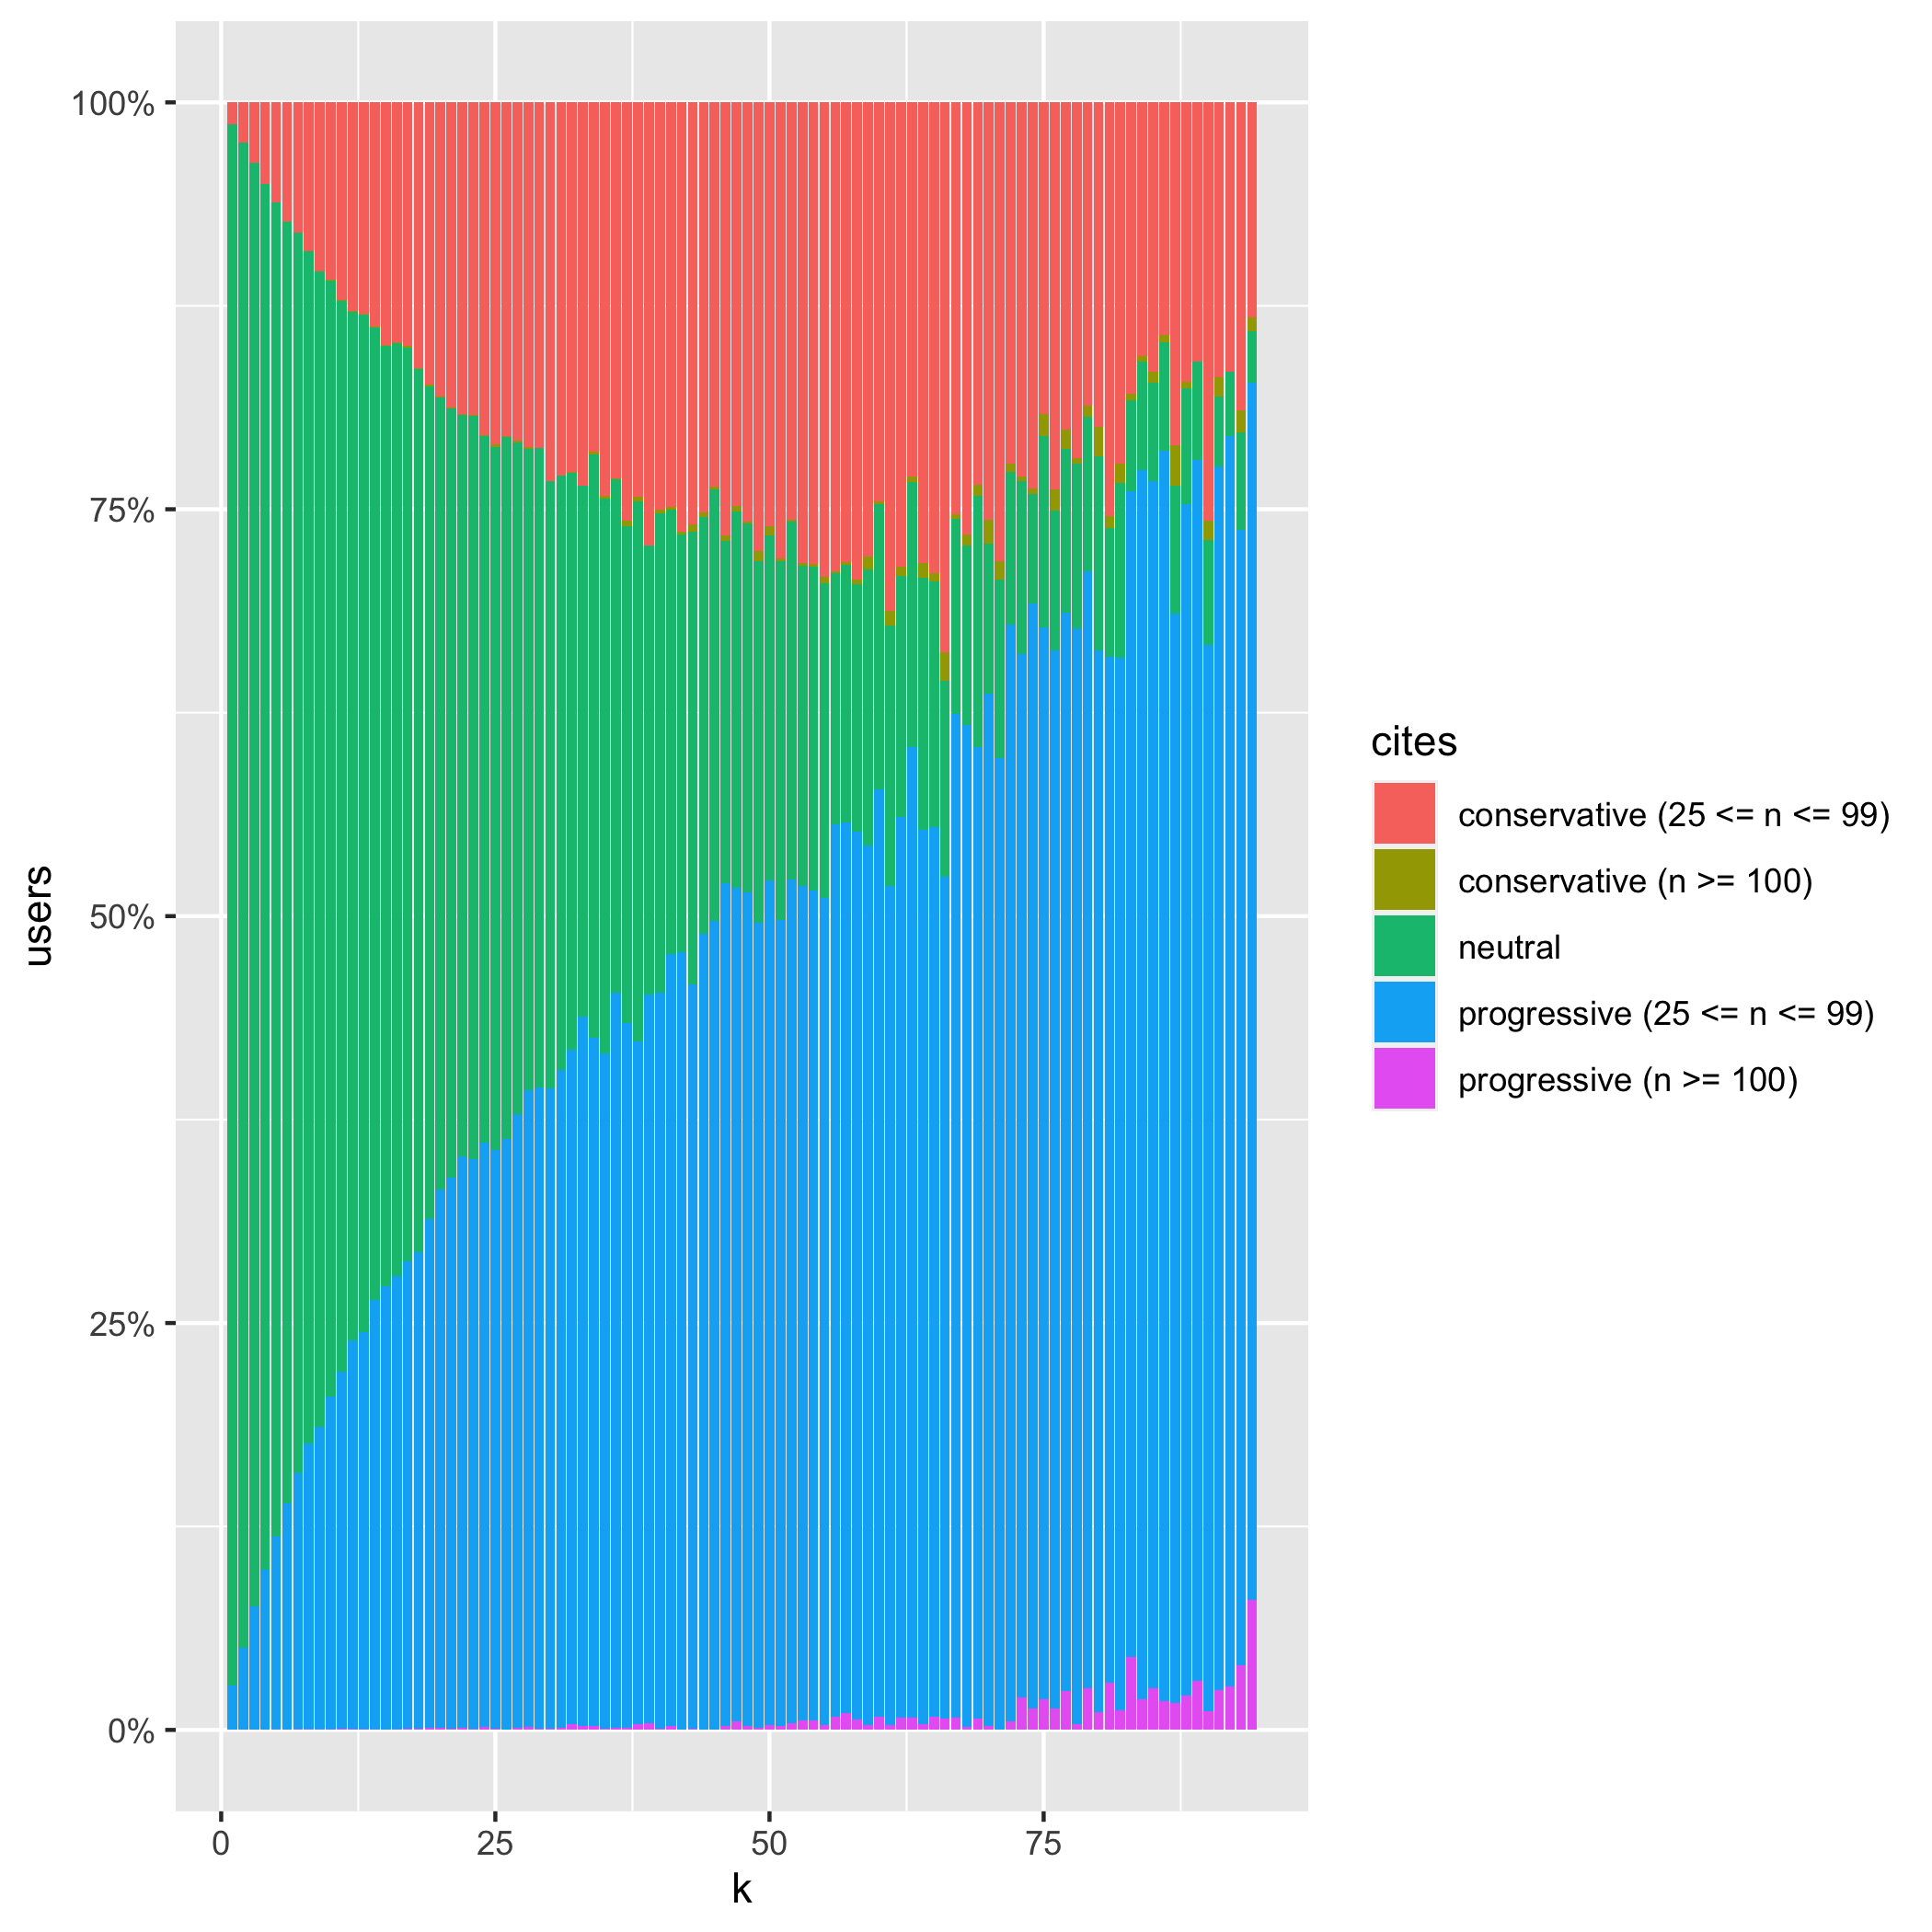
\includegraphics[width=\textwidth]{2016/kshells}
\caption{k-shells}
\label{fig:kshells_2016}
\end{figure}

Figure \ref{fig:kshells_2016} displays the k-core distribution.
The largest-connected component of the user network is composed of 980,390 users.
In total numbers (not depicted), neutral users have an extreme skew to the right with 747,511 (77.28\%) users located in the first 10 shells (on the periphery).
Compared to the previous chapter, the k-cores are much deeper, with 94 shells.
Progressives and conservatives are more distributed in the higher shells; 209 (39.14\%) users with at least 100 progressive cites are found in shells above 90, 47 (17.54\%) users with at least 100 conservative cites are found in shells higher than 80.
Progressive users dominate the higher shells; 1,911 of 2,308 (83\%) in the top k-shell (94) have at least 25 cites of progressive domains.
This clustering of partisan users in the higher shells shows that these partisan sources draw the most engagement, the dominance of progressives hints at the underlying structure of Reddit where a few subreddits such as r/The\_Donald have a dedicated but insular base with fewer users to make connections.

\begin{table}[!ht]
\centering
\footnotesize
\caption{Most ties in top k-shell}
\begin{tabular}{lrrrlrlr}
\toprule
{} & ties & prog & cons & subreddit & cites & dom & cites \\
user &    & cites & cites &         & in    &     & of    \\
\midrule
spsteve             &  1452 &           3 &           0 &    worldnews &       610 &      twitter.com &       466 \\
nohbody123          &  1236 &          11 &           1 &    worldnews &       701 &      twitter.com &       350 \\
catsinbananahats    &  1232 &           2 &           1 &  AskARussian &        23 &       reddit.com &        57 \\
BlatantConservative &  1098 &           4 &           0 &    worldnews &       296 &       reddit.com &       140 \\
Torifyme12          &   990 &           1 &           2 &    worldnews &       117 &      twitter.com &        33 \\
imyourforte         &   988 &           2 &           4 &    worldnews &       778 &    liveuamap.com &       298 \\
InnocentTailor      &   975 &           2 &           0 &    worldnews &       320 &    wikipedia.org &       106 \\
thrae\_awa           &   904 &           4 &           2 &    worldnews &       901 &      twitter.com &       515 \\
LaughingChimera1    &   881 &          10 &           3 &    worldnews &      1016 &      twitter.com &       464 \\
Recidiva            &   868 &           5 &           1 &    worldnews &        96 &    wikipedia.org &        12 \\
mewehesheflee       &   861 &          12 &           1 &    worldnews &       273 &    wikipedia.org &        62 \\
TintedApostle       &   821 &          27 &           8 &    worldnews &       330 &      youtube.com &        81 \\
Wolverinexo         &   821 &           0 &           0 &    worldnews &        26 &    wikipedia.org &        14 \\
haavarl             &   772 &           6 &           1 &    worldnews &       713 &      twitter.com &       382 \\
slothsan            &   757 &           1 &           0 &    worldnews &        88 &      twitter.com &        29 \\
dockneel            &   735 &          86 &           0 &    worldnews &       200 &  theatlantic.com &        86 \\
etzel1200           &   731 &           0 &           2 &    worldnews &       290 &      twitter.com &       180 \\
helm                &   729 &           2 &           0 &    worldnews &        56 &      twitter.com &        14 \\
rishcast            &   709 &          15 &          10 &    worldnews &      1131 &      twitter.com &      1399 \\
TLJDidNothingWrong  &   678 &           7 &           0 &    worldnews &       247 &      twitter.com &       123 \\
Papaofmonsters      &   677 &           0 &           0 &    worldnews &        27 &    wikipedia.org &        19 \\
acox199318          &   674 &           0 &           2 &    worldnews &         8 &      twitter.com &         5 \\
psychoCMYK          &   670 &           6 &           1 &    worldnews &      1025 &    wikipedia.org &       260 \\
oxpoleon            &   653 &           0 &           0 &    worldnews &        58 &    wikipedia.org &        22 \\
SefferWeffers       &   641 &           1 &           1 &    worldnews &        90 &      twitter.com &        22 \\
stirly80            &   641 &           7 &           3 &    worldnews &      2344 &      twitter.com &      1224 \\
yes\_its\_him         &   632 &          10 &           6 &    worldnews &       338 &    wikipedia.org &        60 \\
xmuskorx            &   629 &           2 &           1 &    worldnews &       176 &    wikipedia.org &        81 \\
mbattagl            &   616 &           0 &           0 &    worldnews &        18 &       reddit.com &         7 \\
dianaprd            &   615 &           9 &           0 &    worldnews &       414 &    pravda.com.ua &       151 \\
\bottomrule
\end{tabular}

\label{tab:topk}
\end{table}

The 30 users with the most ties in the top k-shell, as displayed in Table \ref{tab:topk}, seem to confirm this.
17 (56.67\%) users are classified as progressive+ with at least 100 more progressive cites than conservative cites.
Only a single user has more conservative cites than progressive, and only two users prefer a subreddit other than r/politics, r/EnoughTrumpSpam is one of them.
Unlike the rus users, there is not a strong emphasis on Wikipedia and the sources are varied and mainstream.
Having a large number of cites is not a prerequisite for many ties with other users, but only two users have fewer than 150 cites in r/politics.

\begin{table}[!ht]
\centering
\scriptsize
\caption{Users by betweenness centrality}
\begin{tabular}{lrrrrrll}
\toprule
{} & bet & in & out & prog & cons & dom & subreddit \\
user & cent z & deg z & deg z & cites & cites & & \\
\midrule
Galle\_           &      127.97 &     48.62 &      11.77 &          78 &          16 &             reddit.com &             politics \\
loki8481         &      116.72 &     45.82 &      45.14 &         299 &         117 &           politico.com &             politics \\
Lonsdaleite      &      104.37 &     33.85 &      10.15 &         366 &         142 &          wikipedia.org &             politics \\
MaximumEffort433 &       99.80 &     35.03 &      22.34 &        1995 &         153 &     washingtonpost.com &             politics \\
team\_satan       &       96.46 &     24.44 &       4.86 &          30 &           2 &        theguardian.com &  PoliticalDiscussion \\
fastmandan       &       92.08 &     63.01 &      19.33 &          56 &         200 &            youtube.com &           The\_Donald \\
BedWedOrBehead   &       91.85 &     39.99 &       8.37 &          89 &          45 &            youtube.com &             politics \\
reedemerofsouls  &       86.92 &     30.16 &      16.97 &         156 &          38 &             reddit.com &      EnoughTrumpSpam \\
IBiteYou         &       83.80 &     19.70 &      10.05 &         199 &        1428 &             reddit.com &        conservatives \\
Yosarian2        &       83.53 &     56.34 &      14.16 &         282 &          14 &            nytimes.com &             politics \\
Byzantine279     &       80.07 &     37.59 &       8.40 &          29 &           7 &            twitter.com &             politics \\
Block\_Helen      &       78.22 &     31.24 &       5.06 &          18 &          72 &             reddit.com &           The\_Donald \\
joker68          &       76.29 &     19.08 &      29.76 &          78 &        1889 &            youtube.com &           The\_Donald \\
VROF             &       75.51 &     59.49 &      18.38 &        1446 &         114 &     washingtonpost.com &             politics \\
Augustus\_Caesar1 &       72.75 &     32.41 &       8.22 &           2 &           1 &            youtube.com &             politics \\
brainiac3397     &       70.42 &     19.26 &       4.09 &          13 &           1 &          wikipedia.org &             politics \\
druuconian       &       69.35 &     45.48 &      13.64 &         107 &          26 &  realclearpolitics.com &             politics \\
rhino369         &       68.58 &      5.22 &       1.46 &           1 &           0 &            nytimes.com &             politics \\
ademnus          &       68.08 &     52.04 &      22.03 &         650 &         186 &            youtube.com &             politics \\
bottomlines      &       67.89 &     46.82 &      13.68 &          47 &         114 &               youtu.be &             politics \\
Hitchens92       &       67.41 &     14.77 &       2.96 &          66 &          11 &             reddit.com &             politics \\
majorchamp       &       65.73 &     23.27 &      17.87 &          78 &          65 &             reddit.com &             politics \\
watchout5        &       64.15 &     43.21 &      10.73 &          18 &           5 &             reddit.com &             politics \\
veritasserum     &       63.50 &      4.25 &       1.00 &           1 &           8 &             reddit.com &            AskReddit \\
DonnaGail        &       61.00 &     13.88 &       3.64 &           0 &          23 &                redd.it &           The\_Donald \\
rednoise         &       59.38 &     17.13 &       5.10 &         147 &          19 &             reddit.com &  SandersForPresident \\
NachoLawbre      &       58.71 &     34.98 &      10.98 &          90 &          43 &          wikipedia.org &             politics \\
veniceinperil    &       58.64 &     13.27 &       5.50 &          37 &           3 &          wikipedia.org &             politics \\
jacks1000        &       58.14 &     10.23 &       2.86 &          48 &          21 &          wordpress.com &           conspiracy \\
moxy801          &       58.00 &     21.50 &       6.88 &          16 &           3 &             reddit.com &             politics \\
\bottomrule
\end{tabular}

\label{tab:bet_cent}
\end{table}

What about users outside of the top k-shell?
Table \ref{tab:bet_cent} displays the 30 users with the highest betweenness centrality in terms of z-score.
Betweenness centrality is a measure of how often a user is on the shortest path connecting other users, z-scores are the number of standard deviations from the mean.
Of 8 (25.57\%) users with 100 more progressive cites than conservative, 6 favor r/politics and the other two favor r/SandersForPresident and r/EnoughTrumpSpam (multiple users are found in the previous table).
The biggest difference from the top k-shell are 5 (16.67\%) users with more conservative than progressive cites, 3 of which are categorized as conservative+ with 100 more conservative cites than progressive.
These users favor r/The\_Donald and r/conservatives.
We also note the inclusion of r/conspiracy and the varied group of sources.
While the k-core decomposition is primarily a measurement of total connections, the mix of users with high betweenness centrality scores means these users are interacting with users that are in turn interacting with others.
Progressive users populate the most active subreddits such as r/politics, but users of conservative subreddits do interact with users of other subreddits to a lesser extent.

\begin{table}[!ht]
\centering
\scriptsize
\caption{Users by total degree}
\begin{tabular}{lrrrrrll}
\toprule
{} & tot & in & out &  prog &  cons & dom & subreddit \\
user & deg z & deg & deg & cites & cites &                       &                  \\
\midrule
maxwellhill         &     298.70 &      70 &   178793 &         640 &          37 &     independent.co.uk &        worldnews \\
loremipsumchecksum  &     138.67 &     482 &    82615 &         218 &          32 &                qz.com &         politics \\
english06           &     135.48 &     585 &    80602 &          66 &          24 &            reddit.com &         politics \\
Qu1nlan             &     130.63 &    1516 &    76767 &         116 &          32 &            reddit.com &         politics \\
awake-at-dawn       &     123.53 &      20 &    74013 &         109 &          47 &           thehill.com &         politics \\
wonderingsocrates   &     120.23 &     236 &    71823 &         311 &          46 &    washingtonpost.com &         politics \\
saucytryhard        &     115.73 &     338 &    69028 &          80 &          13 &           thehill.com &         politics \\
relevantlife        &     109.92 &     373 &    65518 &         560 &          41 &            reddit.com &         politics \\
WildAnimus          &     102.32 &      73 &    61268 &         295 &         102 &           thehill.com &         politics \\
skoalbrother        &      95.52 &     452 &    56821 &         427 &          37 &             salon.com &         politics \\
NeilPoonHandler     &      93.81 &     196 &    56056 &         640 &           2 &               vox.com &         politics \\
ManiaforBeatles     &      85.07 &      69 &    50953 &         151 &          13 &     independent.co.uk &        worldnews \\
therecordcorrected  &      83.25 &    1892 &    48039 &        5843 &          85 &           twitter.com &  EnoughTrumpSpam \\
imagepoem           &      82.77 &    1209 &    48433 &         118 &          80 &           thehill.com &         politics \\
DrJarns             &      81.54 &    2509 &    46397 &         127 &        5276 &  thegatewaypundit.com &       The\_Donald \\
The-Autarkh         &      80.36 &    3617 &    44586 &         618 &          36 &    washingtonpost.com &         politics \\
progress18          &      80.22 &     153 &    47966 &        1206 &          24 &           twitter.com &   hillaryclinton \\
Antinatalista       &      78.92 &     394 &    46945 &         292 &           1 &     independent.co.uk &         politics \\
cyanocittaetprocyon &      77.42 &    1350 &    45090 &         373 &           4 &           thehill.com &         politics \\
viccar0             &      77.02 &    2010 &    44191 &         222 &          49 &    washingtonpost.com &         politics \\
DrWeeGee            &      76.55 &    1110 &    44809 &          87 &         282 &            reddit.com &       The\_Donald \\
Usawasfun           &      76.04 &    3424 &    42193 &         142 &          48 &    washingtonpost.com &         politics \\
madam1              &      74.79 &      83 &    44784 &        1050 &           1 &           reuters.com &         politics \\
PikachuSquarepants  &      72.58 &    1144 &    42403 &         112 &           4 &        politifact.com &         politics \\
Shitposter123456789 &      71.85 &     947 &    42163 &         191 &         316 &           twitter.com &         politics \\
mvea                &      68.64 &      17 &    41168 &         339 &          15 &       theguardian.com &       Futurology \\
sivribiber          &      67.74 &      26 &    40621 &         187 &           8 &    washingtonpost.com &         politics \\
SimulationMe        &      66.09 &     173 &    39491 &         370 &          10 &           thehill.com &         politics \\
wenchette           &      65.20 &    2975 &    36153 &        1457 &          55 &    washingtonpost.com &   hillaryclinton \\
anutensil           &      63.91 &     273 &    38086 &        2257 &           5 &     thinkprogress.org &        democrats \\
\bottomrule
\end{tabular}

\label{tab:tot_deg}
\end{table}

Finally, \ref{tab:tot_deg} displays the 30 users with the highest total degree, or combined incoming and outgoing connections.
Out-degree dwarfs in-degree; the user with the most incoming connections (3,617) has 44,680 outgoing connections.
21 (70\%) users are categorized as progressive+, 17 prefer r/politics, though r/hillaryclinton, r/democrats, and r/worldnews are also present.
3 (10\%) users are conservative+, two of them prefer r/The\_Donald and one prefers r/politics.
These are all very active users with large numbers of comments, replies, and cites.
We note u/therecordcorrected, an allusion to a Clinton-favoring astroturfing campaign, Correct the Record.
More interesting is the presence of u/maxwellhill with more than double the out-degree of the next user.
When Jeffrey Epstein and his confidant Ghislaine Maxwell were arrested in 2019, the user, active as a moderator on numerous subreddits, became the target of a conspiracy theory which suggested they were Maxwell.
Of course this user would have the power to influence activity on the site, but the sheer numbers suggest not a part-time user that dabbled in Reddit on the side, but rather someone that spent substantial time and effort, to an extent that does not match what we know of Maxwell's social and public life.

\subsection{Textual Analysis}

For the textual analysis we could take a similar approach as the previous chapter where we tracked the influence of superspreaders of Russian propaganda, comparing the most progressive users (progressive+) with the most conservative users (conservative+) and seeing how they appear to influence discussion.
Given that chapter's findings, we might expect these users posting the most partisan material would attract discussion in any context, especially because they post so much of it.
How much these users drive discussion is probably dependent on where the discussion is happening: progressive users posting in r/The\_Donald may draw attention the same way anyone who stands out will, but with the number of diehards they are posting against and the obvious orientation of that subreddit, their influence will be limited, and vice versa for conservative users posting in progressive environments.
Subreddits like r/worldnews or r/news should provide the most opportunity for driving discussion, even given Reddit's apparent progressive tilt.

However, the user groups in this chapter are different in several ways which present other more interesting paths of analysis.
In the Russia example, users either were pro-Russia or neutral, posting favorable content or the absence of it, but not two groups with competing, explicit parties.
The Russian context is also an international one with users very aware of and informed on the situation (even if with a slant) interacting with others with limited awareness or interest in Crimea or Ukraine.
In the United States, the election of the president is much more important and salient for the average person and almost everyone will have some knowledge of and opinion on it.
With partisanship at perceived highs, the us vs them nature of the first-past-the-post, two-party system, and the seeming ability of the tail to wag the dog (or strong partisans having outsized influence in the Internet age), it is useful to see how progressives and conservatives see each other.
Do these groups oppose a reality, or are they shadow boxing with opponents they have constructed?

The setup is straightforward.
We take the progressive+ and conservative+ groups discussed previously and defined in Table \ref{tab:2016_groups} and train Word2vec models for each, capturing the topics discussed by these most partisan and active of users.
For progressives, we query for the 300 most-similar terms for ``conservative'', and for conservatives, the 300 most-similar terms for ``progressive''.
t-SNE is used for dimensionality-reduction to produce a 2D graph, and k-means to cluster closely-related terms.
The reduction from 300 to 2 dimensions means that information is lost and we are only viewing a thin slice or perspective of the data and as such there is no optimal form of clustering.
However, similar clusters persist across multiple runs and settings and the k-means provide reasonable divisions of topics.

Before continuing, we note that similarity in the Word2vec context has multiple meanings.
Terms can be those used in the same sentence or paragraph but with opposing meanings (Democrat and Republican), or with the intention of describing each other (Republican and Conservative).
Fascist and communist may be grouped together but that does not necessarily mean that they are synonyms within the model.
Word2vec is only a measure of physical proximity within the text, as are the k-means clusters derived from it.
The graph of 300 talking points for a given term are the 300 words most commonly used in proximity to it, the clusters are the words within used most often with each other.
Clusters are used to focus on topics, but they are not definite and they do not have any relationship across graphs other than being similar.
Modern tools such as BERT are designed to capture context and meaning in a much more nuanced way, but these Word2vec models are a useful starting point.

\begin{figure}[!ht]
\centering
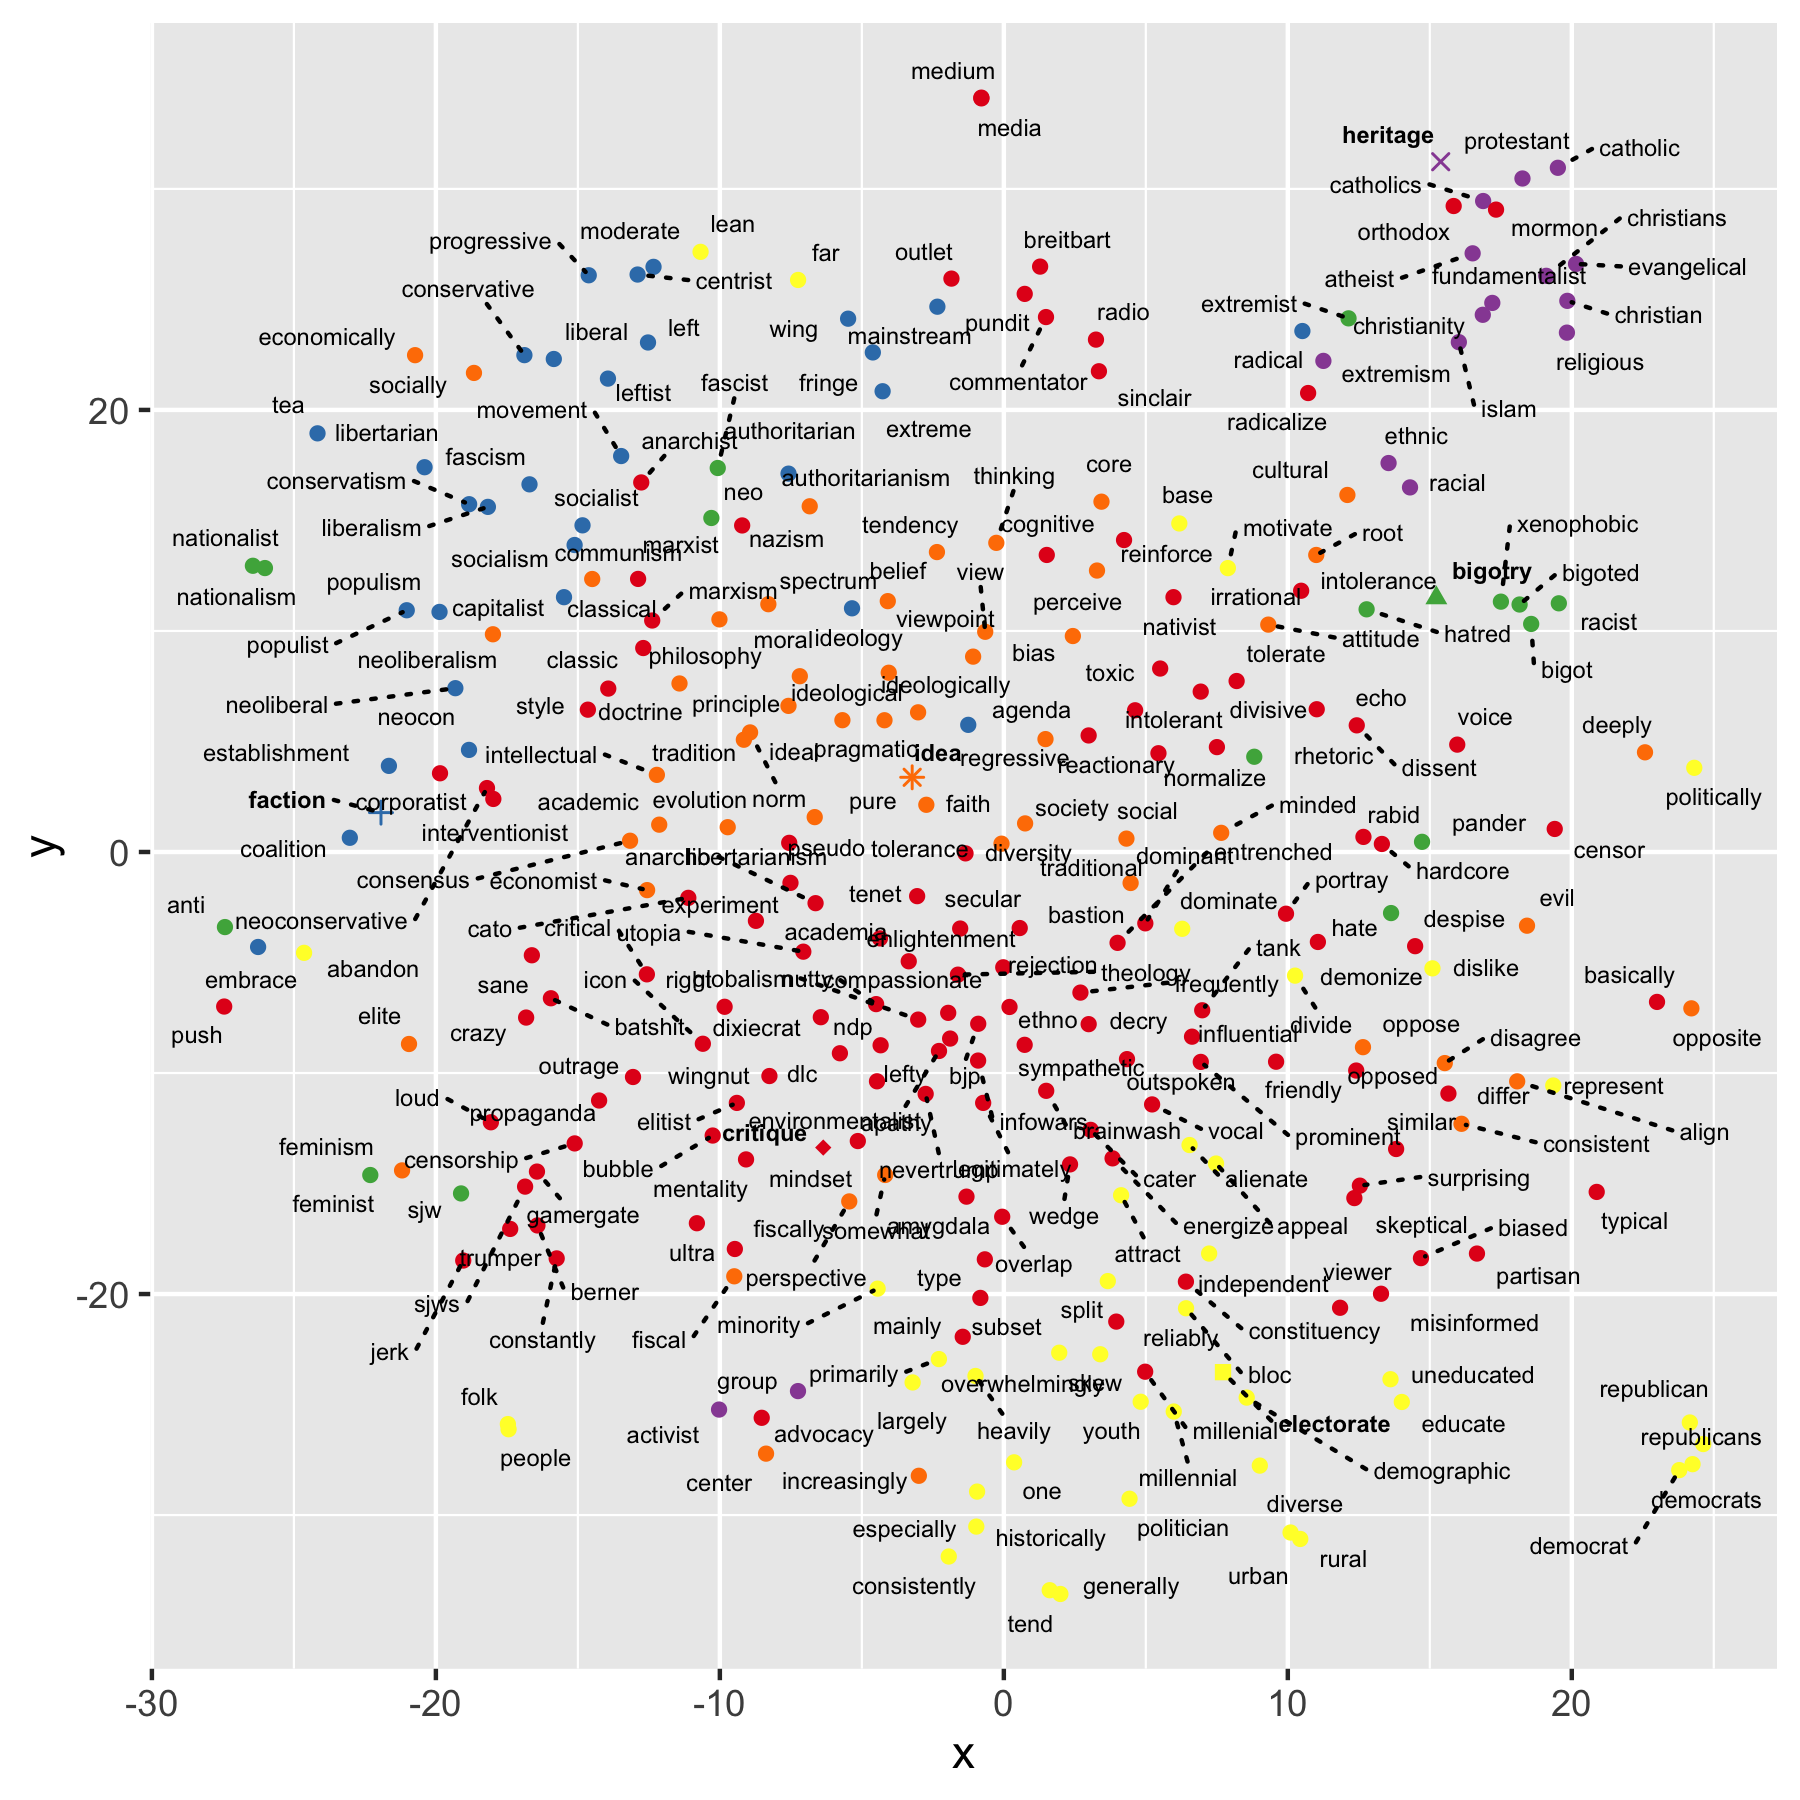
\includegraphics[width=\textwidth]{2016/prog_plus_conservative}
\caption{Most-similar to ``conservative'' (progressive+)}
\label{fig:prog_plus_cons}
\end{figure}

Figure \ref{fig:prog_plus_cons} displays the 293 most-similar terms to ``conservative'' for the progressive+ users.
Individuals are removed in order to avoid cross-cutting clustering across people and things, and several non-grammatical terms due to bad word splits have been filtered out as well.
However, only four people are filtered: Rupert Murdoch, Rush Limbaugh, and the Koch brothers, which suggests the personalities seen as most responsible for the following, or perhaps the progressive+ group's representative conservative.

In the top-left is the ``faction'' cluster containing political stances: \emph{agenda, authoritarian, capitalist, centrist, coalition, conservatism, embrace, establishment, extreme, faction, fascism, fringe, ideology, left(ist), liberal(ism), libertarian, mainstream, moderate, movement, neocon, neoliberal, populism, progressive, radical, socialism, tea, wing}.
In the opposite bottom-right corner is the ``electorate'' cluster discussing voters: \emph{abandon, alienate, appeal, attract, base, bloc, democrat(s), demographic, dislike, diverse, divide, dominate, educate, electorate, far, folk, generally, heavily, historically, independent, largely, lean, millennial, minority, motivate, overwhelmingly, people, politician, primarily, represent, republican(s), rural, skew, split, tend, uneducated, urban, youth}.
Both groupings with their variety of terms suggest comparison and do not have an obvious tilt. 

The top-right corner has the ``heritage'' cluster with terms related to group identities: \emph{activist, atheist, catholic(s), christian(s), christianity, ethnic, evangelical, extremism, fundamentalist, group, heritage, islam, protestant, racial, religious}.
Beneath it is a smaller ``bigotry'' cluster focused on targets and negative effects of tradition: \emph{anti, bigotry, extremist, fascist, feminist, hate, nationalism, neo, pander, racist, rhetoric, sjw, xenophobic}.
We note the inclusion of ``fundamentalism'' and ``extremism''  as qualifiers.

The remaining clusters are the largest with the least topic definition.
Towards the center of the plot is the ``idea'' cluster emphasizing the abstract and intellectual: \emph{academic, align, attitude, authoritarianism, belief, bias, center, communism, consensus, consistent, core, cultural, deeply, disagree, diversity, doctrine, economically, economist, elite, evil, evolution, faith, feminism, fiscal, idea(l), ideological(ly), increasingly, intellectual, minded, moral, neoliberalism, norm, oppose, opposite, perceive, perspective, philosophy, pragmatic, principle, pure, regressive, root, social(ly), society, somewhat, spectrum, tendency, thinking, tradition(al), view(point)}.
Many of these terms overlap with terms in other groups: communism, faith, and regressive could easily fit in the preceding three clusters.

Finally, the ``critique'' cluster in the bottom-left of the graph contains many of the most negative associations, including: \emph{apathy, batshit, biased, brainwash, breitbart, bubble, censor(ship), corporatist, crazy, decry, demonize, despise, dissent, divisive, dixiecrat, echo, elitist, entrenched, ethno, gamergate, globalism, hardcore, intolerant, irrational, jerk, misinformed, nazism, nutty, partisan, propaganda, pseudo, rabid, radicalize, reactionary, rejection, skeptical, tank, toxic, ultra, wedge, wingnut}.
We also note a number of terms related to mass media and partisan commentary: \emph{breitbart, cato, commentator, infowars, media, outlet, outrage, outspoken, pundit, radio, sinclair, viewer, voice}.

Without reading more into the graph than the words used, the old struggle of traditional versus progressive values and belief systems is dominant.
There are undeniably negative notions like irrationality, intolerance, and terms like rabid or nutty, but we cannot determine whether these terms only apply to conservatives or include other groups along the spectrum.
The criticism is closely connected to ``extremism'', which cannot be defined but seems associated with talk radio and new media like Breitbart and InfoWars, especially considering the removed individuals' importance to that media ecosystem.

\begin{figure}[!ht]
\centering
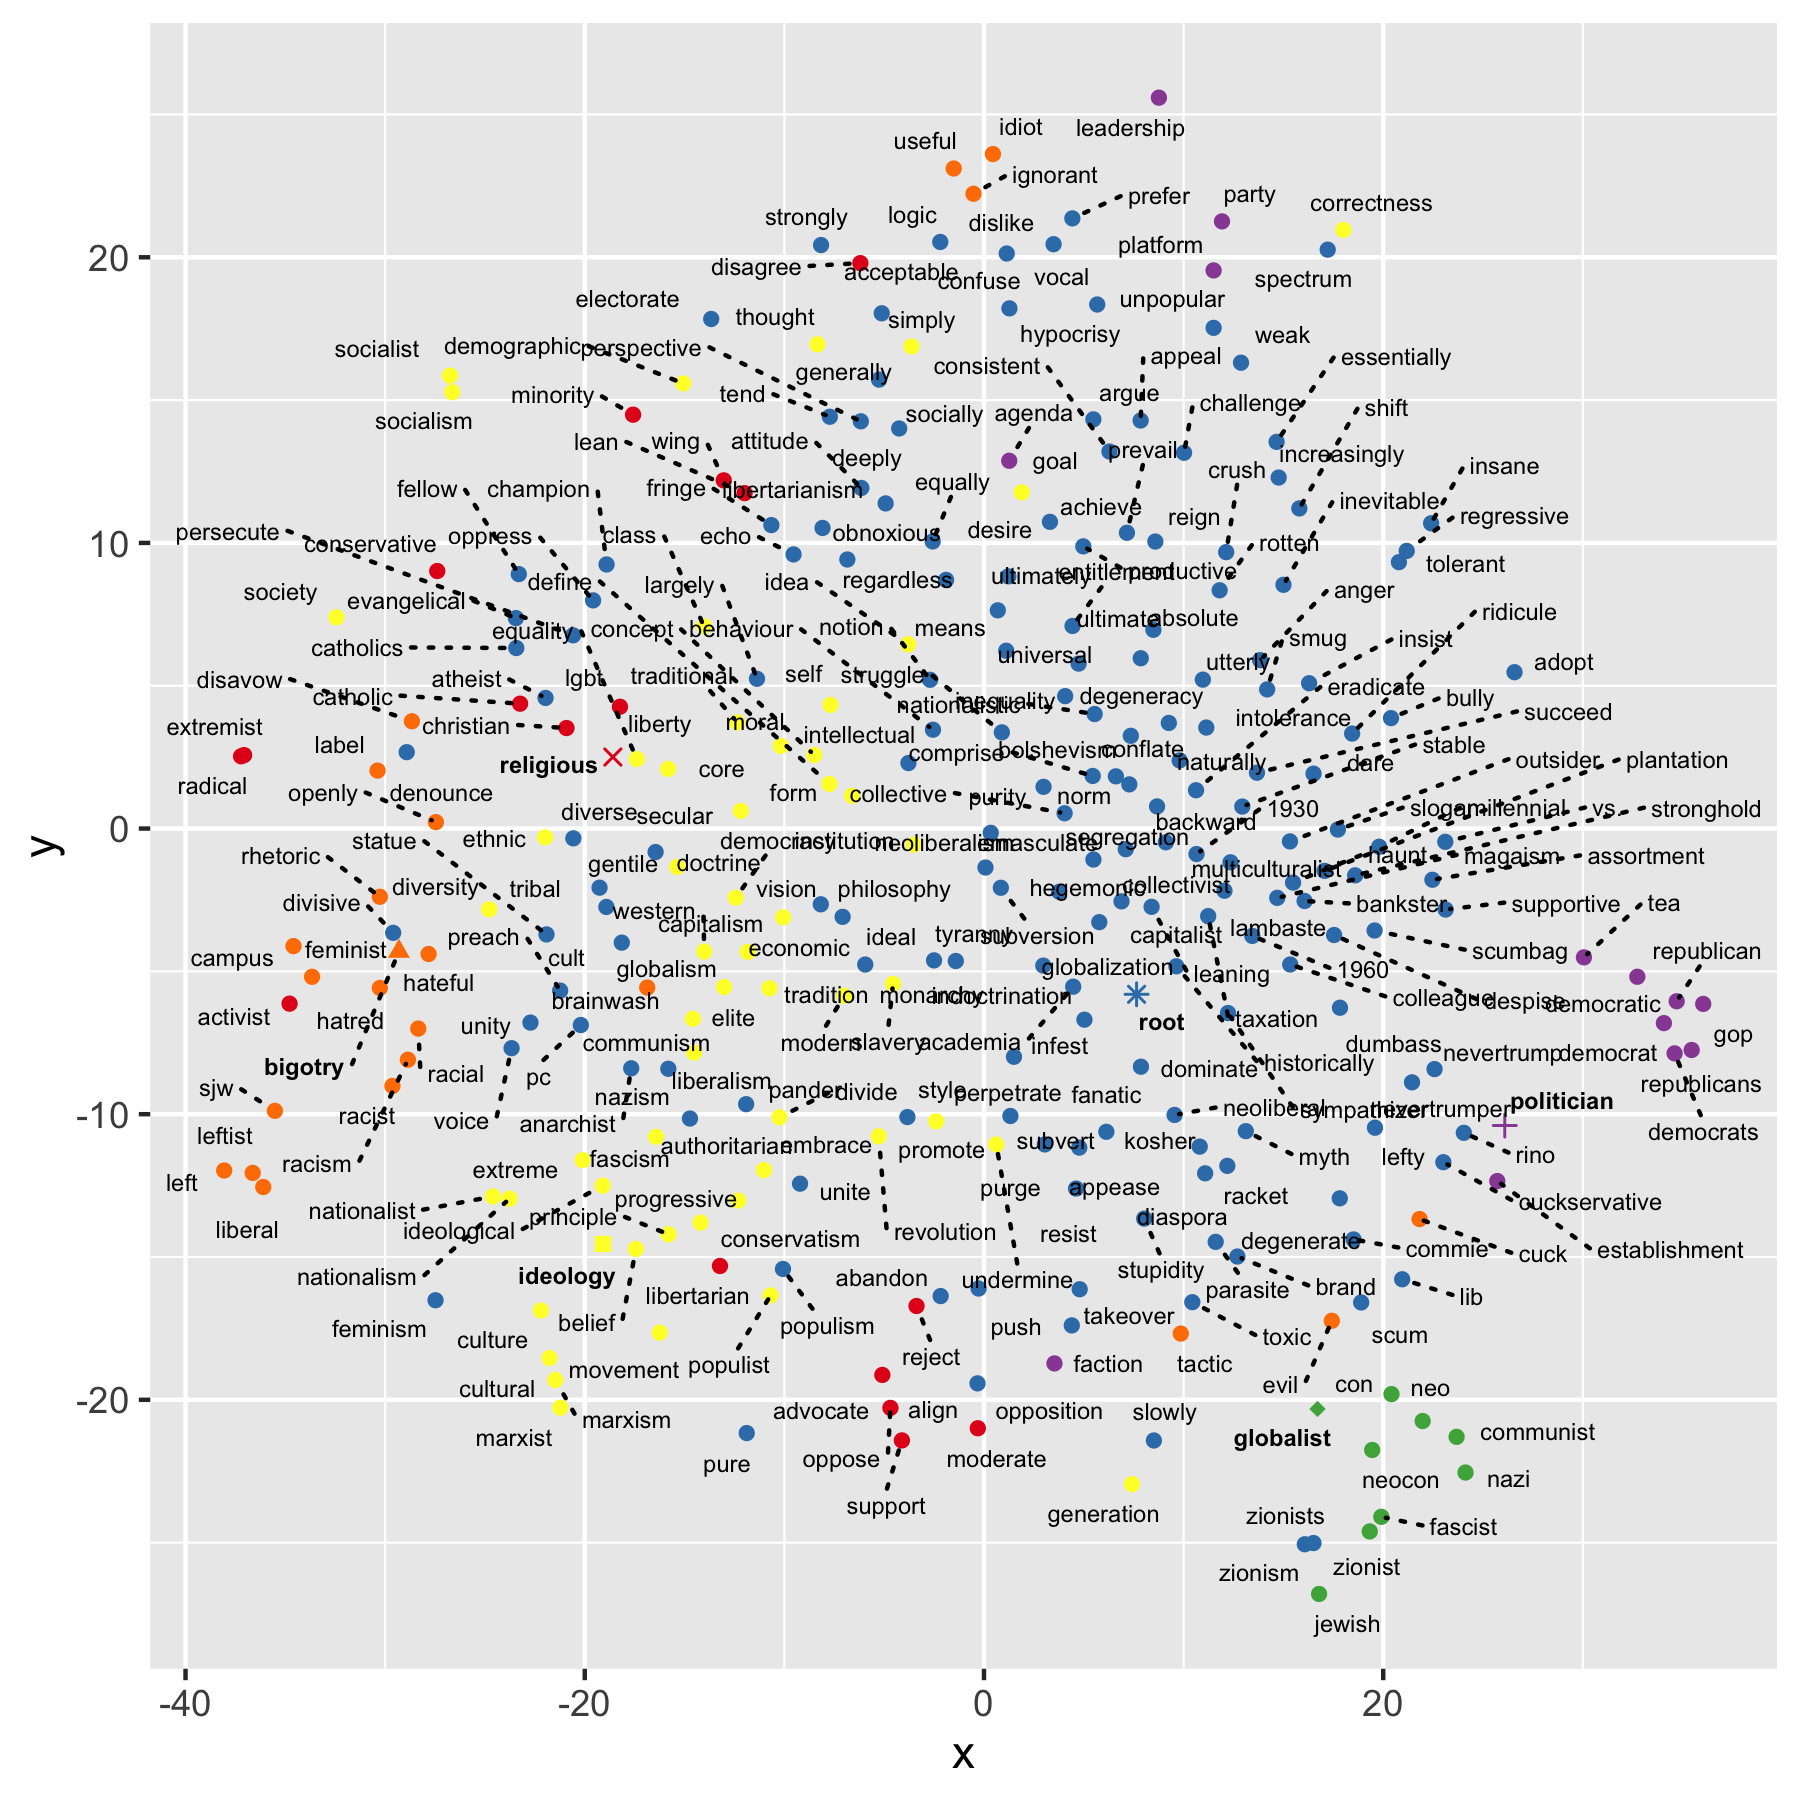
\includegraphics[width=\textwidth]{2016/cons_plus_progressive}
\caption{Most-similar to ``progressive'' (conservative+)}
\label{fig:cons_plus_prog}
\end{figure}

We now flip the group and term in order to examine users on the other end of the political spectrum.
Figure \ref{fig:cons_plus_prog} displays the 297 most-similar terms to ``progressive'' for the conservative+ users.
One term is removed due to being ungrammatical and only two individuals are filtered out: Bernie Sanders and Hitler.

The clusters in this plot have no direct relationship with the previous, but there are similarities in grouping.
One grouping shared with the progressive plot is a variety of political positions and ideologies.
This ``belief'' cluster, located towards the bottom-left, includes the terms: \emph{belief, capitalism, class, communism, concept, conservatism, core, correctness, culture, democracy, demographic, diversity, divide, doctrine, economic, elite, embrace, equality, ethnic, extreme, fascism, form, generation, globalism, goal, idea, ideology, institution, liberalism, liberty, marxism, modern, moral, movement, nationalism, populist, principle, progressive, promote, revolution, self, slavery, socialism, society, thought, traditional, undermine, western}.

There are multiple other similar clusters, a smaller ``politician'' cluster on the right side of the graph refers to Democrats and Republicans explicitly.
Found within are the terms: \emph{agenda, democrat(s), democratic, establishment, gop, leadership, opposition, party, platform, politician, republican(s), tea}.
At the top-left is a ``religious'' cluster including: \emph{activist, advocate, catholic, christian, conservative, disagree, extremist, lean, lgbt, libertarian, minority, moderate, oppose, radical, reject, religious, support, wing}. 
``Bigotry'' and other potential negatives of identities are grouped on the left side with: \emph{bigotry, brainwash, campus, cuck, disavow, evil, feminist, hatred, idiot, ignorant, label, left(ist), liberal, openly, racial, racism, rhetoric, sjw, tactic, useful}.
To the bottom-right is the ``globalization'' cluster of political extremes and terms adjacent to Israeli politics: \emph{communist, con, fascist, globalist, jewish, nazi, neo, neocon, zionist}.

Finally, the ``root'' cluster in the center of the graph covers many topics and is the least well-defined, suggesting these terms are used in a variety of contexts.
Some of the more negative or notable are: \emph{authoritarian, backward, bankster, bolshevism, bully, commie, conflate, confuse, crush, cuckservative, cult, degeneracy, denounce, despise, dislike, divisive, dominate, dumbass, echo, emasculate, eradicate, fanatic, haunt, hegemonic, hypocrisy, indoctrination, inequality, infest, insane, intolerance, lambaste, myth, nazism, obnoxious, oppress, pander, parasite, pc, persecute, plantation, purge, racket, regressive, resist, ridicule, rino, rotten, scum(bag), segregation, smug, struggle, stupidity, subvert, takeover, toxic, tribal, tyranny, unpopular, vs., weak, zionism}.
Of course, we do not know the exact context these terms were used within and the entire cluster includes neutral and positive terms.
We select these with an emphasis on ``othering'' language like degenerate, scum, parasite, and rotten, likely derived from Trump's populist rhetoric.

Both groups, progressive and conservative use similar terms and have similar clustering of topics such as religion.
There are only so many political issues to cover but this at least indicates shared interests if not views.
Each group shows apparent concern over top-down elite negative influences.
Progressives seem more worried about this from media; conservatives use more populist language of banksters, academia, globalists, and Zionists.

Using these graphs of talking points we have some idea of how these groups see each other and the wider political environment.
How do these views affect the interpretation of specific events?
In order to analyze this, we observe the reaction to the Mueller investigation into Trump's ties with Russia and related issues discussed at the beginning of this chapter.
For many conservatives, the ongoing investigation and the Steele dossier, alleged Russian kompromat from 2017, have become known as ``Russiagate''.
The initial overstated claims of the dossier were effective at discrediting the later substantial findings of Mueller's report, which given the historical use of Soviet and Russian active measures may have been the point.

\begin{figure}[!ht]
\centering
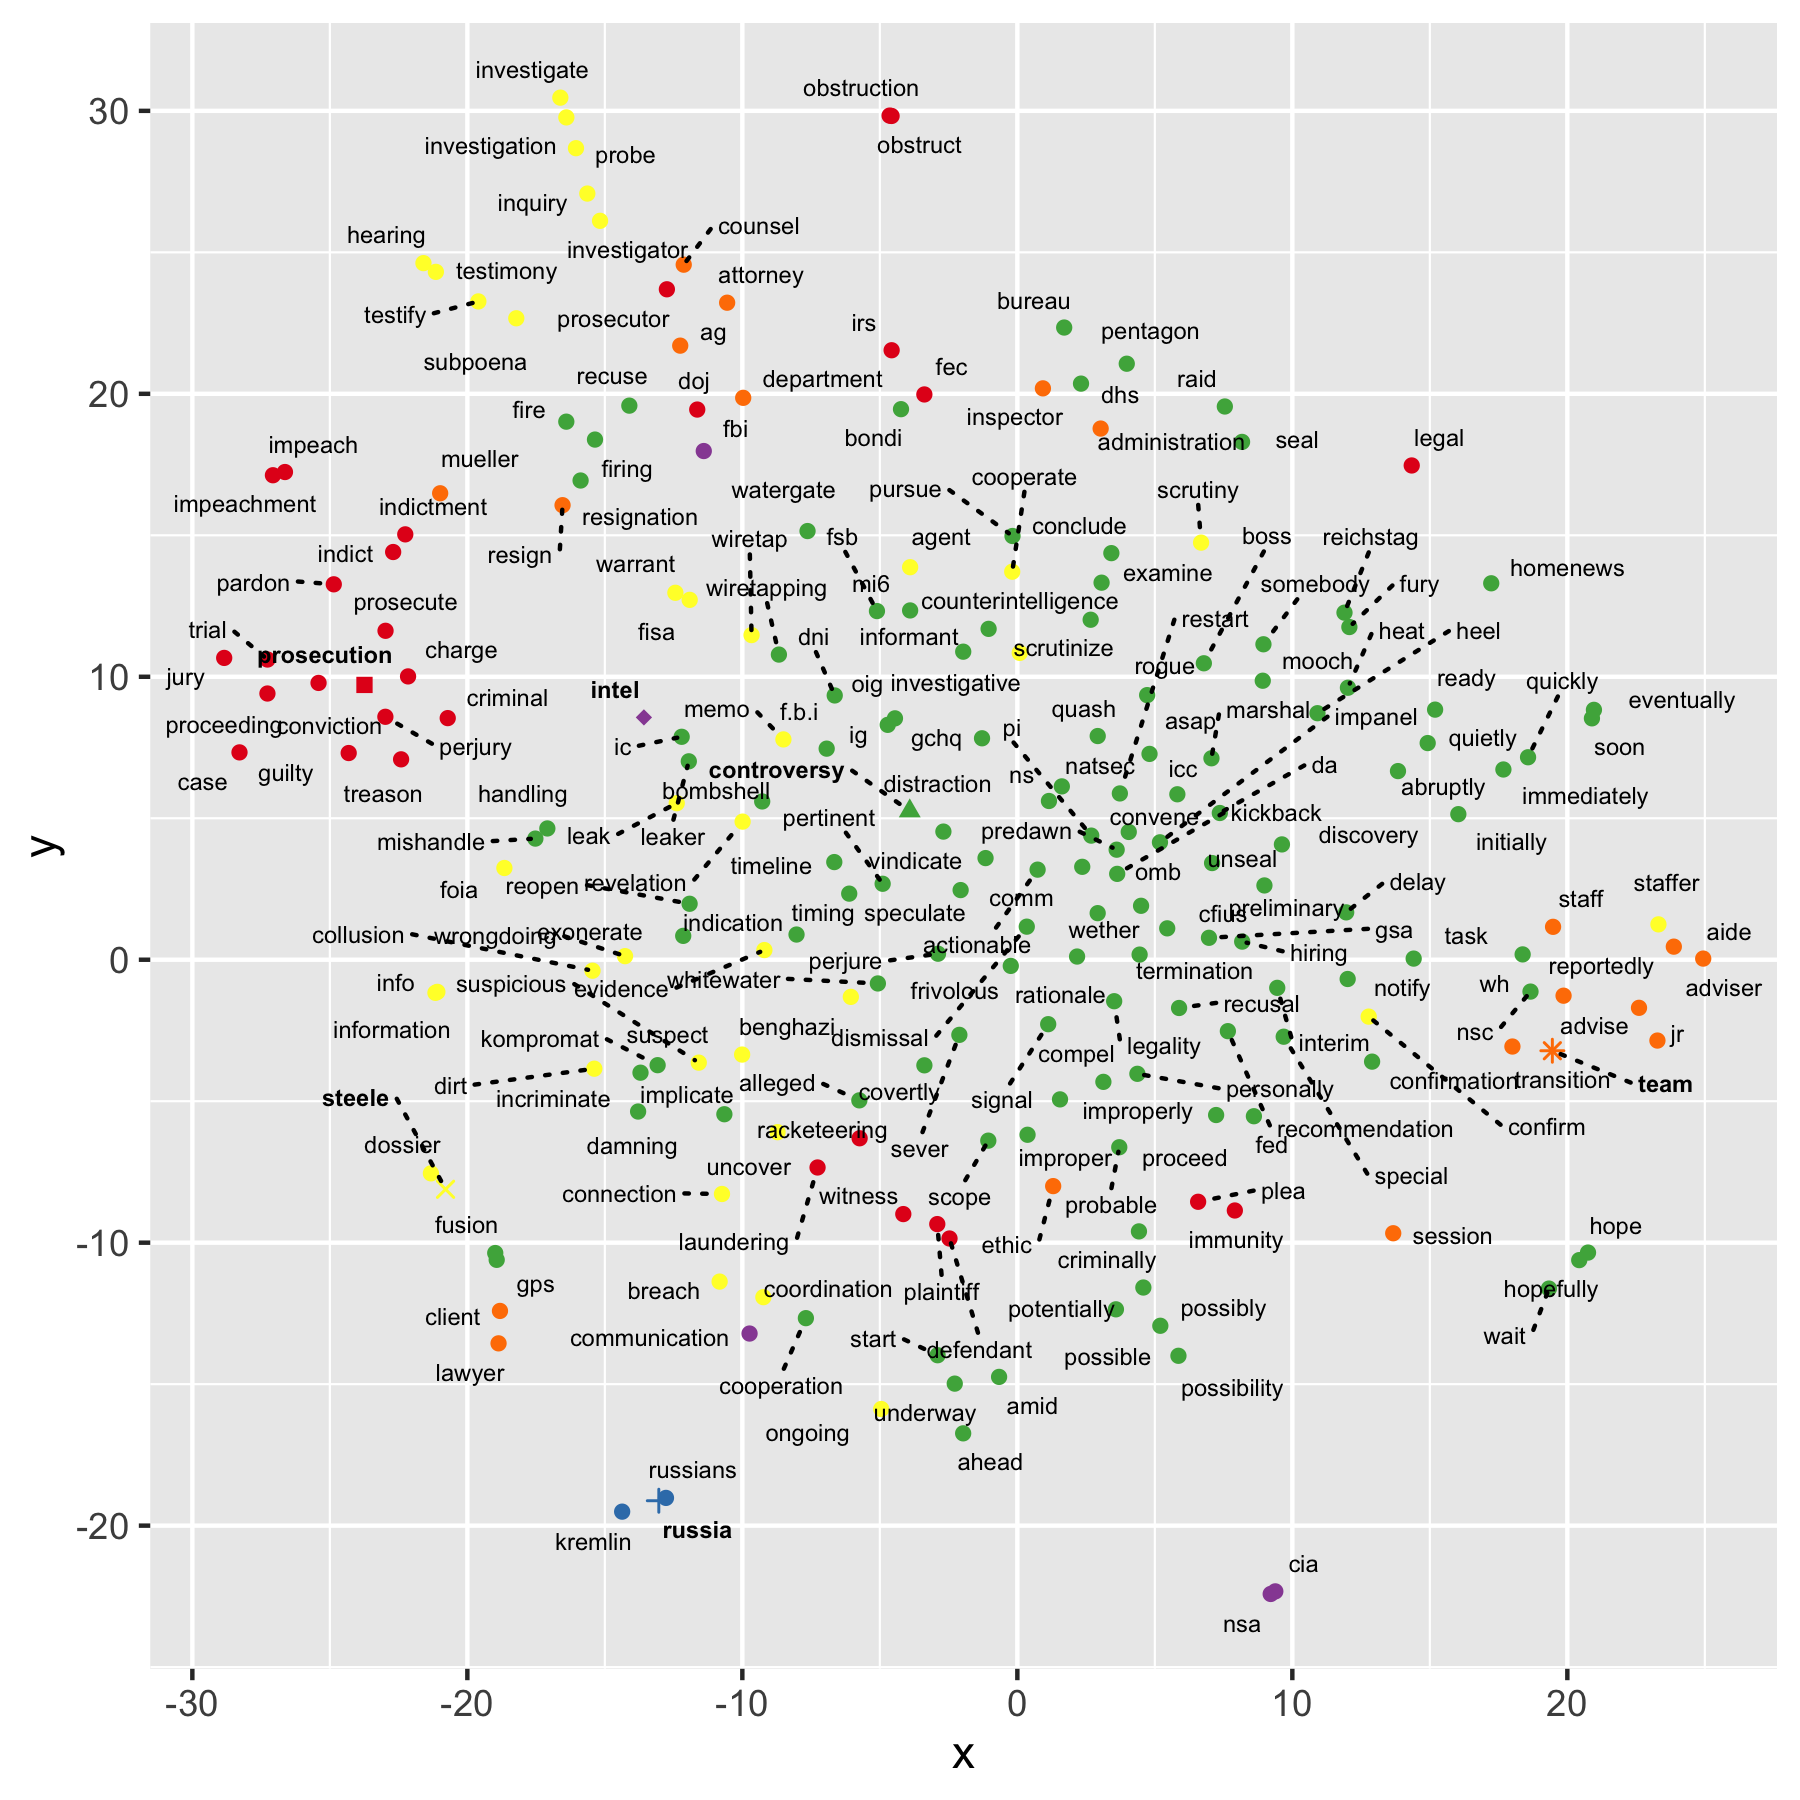
\includegraphics[width=\textwidth]{2016/prog_plus_mueller}
\caption{Most-similar to ``Mueller'' (progressive+)}
\label{fig:prog_plus_mueller}
\end{figure}

Russiagate is used so infrequently by progressives that it does not show up in the vocabulary of the trained progressive+ model.
Figure \ref{fig:prog_plus_mueller} displays the 227 most-similar terms to Mueller for the progressive+ group.
The much larger number of individuals removed is due to the many whistleblowers, news sources, and political actors involved.
We do not remove Mueller or Steele, session (Jeff Sessions, Trump's Attorney General), jr (Donald Trump, Jr.), or mooch (Anthony Scaramucci); the final three are ambiguous.

Smaller peripheral clusters include the ``Russia'' cluster at the bottom-left: \emph{kremlin, russia(ns)}, the Trump ``team'' cluster to the right: \emph{administration, advise(r), ag, aide, attorney, client, counsel, department, ethic, inspector, jr, lawyer, mueller, reportedly, resign, session, staff, team, transition}, and the ``intel'' cluster found towards the top-left and bottom-right: \emph{cia, communication, fbi, intel, nsa}.

The ``prosecution'' and ``Steele'' clusters on the left are similar with terms like prosecutor, prosecution, investigation but the former explicitly mentions the dossier and contains terms central to the end Mueller findings regarding coordination or collusion.
The first includes: \emph{case, charge, conviction, criminal, defendant, doj, fec, guilty, immunity, impeach(ment), indict(ment), irs, jury, laundering, legal, obstruct(ion), pardon, perjury, plaintiff, plea, proceeding, prosecute, prosecution, prosecutor, racketeering, treason, trial, witness}.
The Steele cluster contains: \emph{agent, benghazi, breach, collusion, confirm, connection, cooperate, coordination, dirt, dossier, evidence, fisa, foia, hearing, info(rmation), inquiry, investigate, investigation, investigative, investigator, leak, memo, ongoing, probe, revelation, scrutiny, staffer, steele, subpoena, suspect, suspicious, testify, testimony, uncover, warrant, wiretap, wrongdoing}.

Finally, the center cluster details much of the ``controversy'': \emph{actionable, alleged, bombshell, bondi, boss, bureau, compel, conclude, confirmation, controversy, cooperation, counterintelligence, covertly, criminally, da, damning, delay, dhs, discovery, dismissal, distraction, dni, examine, exonerate, f.b.i, fed, firing, frivolous, fsb, fury, fusion, gchq, gps, gsa, handling, heat, heel, hope, ic(c), ig, impanel, implicate, improper(ly), incriminate, informant, kickback, kompromat, leaker, legality, marshal, mi6, mishandle, mooch, natsec, ns(c), oig, omb, pentagon, perjure, pertinent, pi, possibility, potentially, preliminary, probable, pursue, quash, quietly, raid, rationale, recommendation, recusal, reichstag, resignation, rogue, scope, scrutinize, seal, sever, special, speculate, termination, timeline, timing, unseal, vindicate, watergate, wh, whitewater, wiretapping}.
This cluster and the graph as a whole do not appear especially biased or colored.
Without prior knowledge of the events, these terms are obviously discussing a serious ongoing political investigation.
The desire for findings of treason or impeachment could perhaps be read into it, but with terms like exonerate and frivolous, it is not clear this is expected.

\begin{figure}[!ht]
\centering
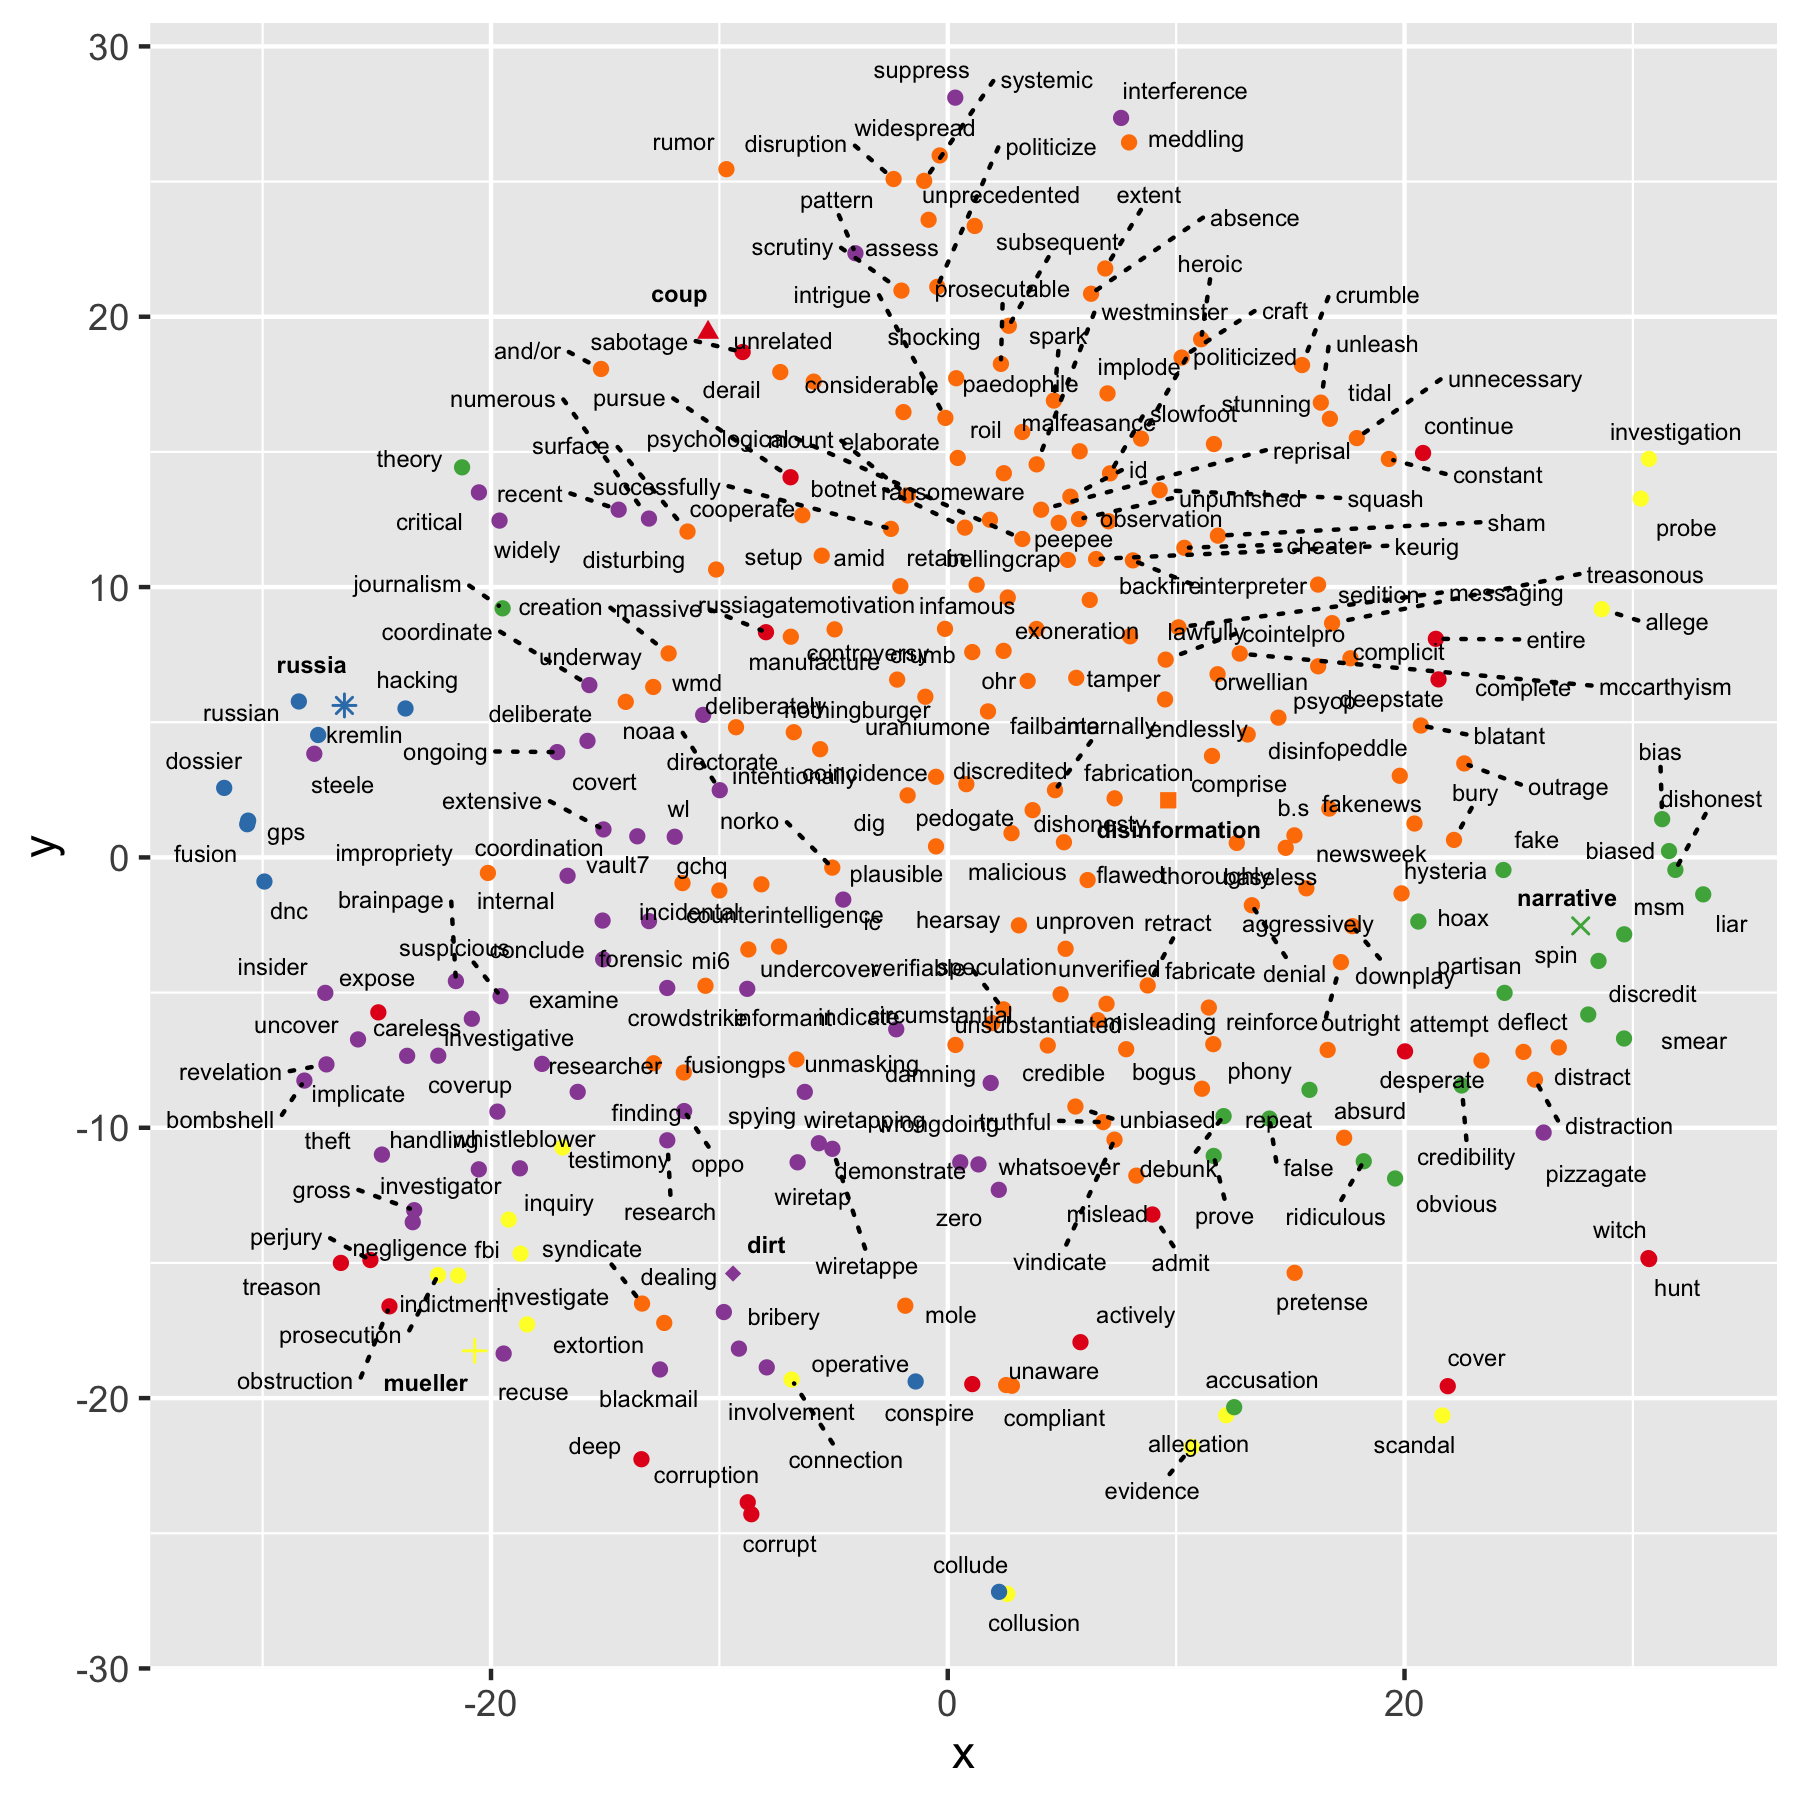
\includegraphics[width=\textwidth]{2016/cons_plus_russiagate}
\caption{Most-similar to ``Russiagate'' (conservative+)}
\label{fig:cons_plus_russiagate}
\end{figure}

Figure \ref{fig:cons_plus_russiagate} displays the 283 most-common terms to Russiagate for the conservative+ group with 9 individuals removed.
We begin with a familiar ``Russia'' cluster, found on the left side: \emph{collude, dnc, dossier, fusion, gps, hacking, kremlin, operative, russia(n)}.
This includes the hacking of the DNC in 2016, which is not emphasized in the progressive talking points; the entire conservative plot mentions Fusion GPS, the firm behind the Steele dossier, multiple times.

On the periphery are multiple clusters about the investigation, the progressive plot has a similar split.
In the bottom-left corner, the ``Mueller'' cluster is the most straightforward and factual: \emph{allegation, collusion, connection, evidence, fbi, indictment, investigate, investigation, investigator, mueller, probe, prosecution, scandal, testimony}.
Collusion and connection are part of the specific legal verbiage used in the 2018 report.
The ``coup'' cluster (top-left, edges of plot) has related terms like conspire, corrupt, and perjury, but the presence of coup and witch (hunt) flips the investigation onto the accusers: \emph{actively, admit, attempt, conspire, corrupt(ion), coup, cover,  deep, expose, hunt, massive, obstruction, perjury, pursue, sabotage, treason, witch}.
Claims of bias are reiterated in the ``narrative'' cluster to the right, skeptical of the narrative and media more generally: \emph{accusation, bias(ed), credibility, debunk, discredit, dishonest, fake, false, hoax, journalism, liar, msm, narrative, obvious, partisan, prove, repeat, ridiculous, smear, spin, theory}.

Finally, the  ``dirt'' (center-left) and ``disinformation'' (center) clusters contain a variety of relevant details along with unrelated conspiracies (Pizzagate), extreme claims (Orwellian, deepstate, McCarthyism), and dubiousness (nothingburger).
Some of the first cluster terms are: \emph{blackmail, bombshell, bribery, careless, conclude, coordination, covert, coverup, critical, crowdstrike, dirt, examine, extensive, finding, forensic, gross, handling, ic, implicate, indicate, informant, inquiry, insider, interference, internal, investigative, involvement, negligence, noaa, numerous, ongoing, oppo, pattern, pizzagate, recuse, research, revelation, spying, steele, suppress, suspicious, theft, uncover, whatsoever, whistleblower, widely, wiretap(pe), wiretapping, wl, wmd, wrongdoing, zero}.
The second and largest cluster includes: \emph{absence, absurd, aggressively, assess, b.s, backfire, baseless, bellingcrap, blatant, bogus, botnet, bury, cheater, circumstantial, coincidence, cointelpro, compliant, complicit, controversy, cooperate, counterintelligence, craft, creation, credible, crumb(le), damning, deepstate, deflect, deliberate(ly), denial, derail, desperate, dig, discredited, dishonesty, disinfo(rmation), disruption, distract(ion), disturbing, downplay, elaborate, endlessly, exoneration, extortion, fabrication, failbama, fakenews, flawed, fusiongps, hearsay, heroic, hysteria, implode, impropriety, incidental, infamous, intentionally, internally, intrigue, lawfully, malfeasance, malicious, manufacture, mccarthyism, meddling, messaging, mi6, mislead(ing), mole, motivation, mount, newsweek, norko, nothingburger, ohr, orwellian, outrage, outright, paedophile, peddle, pedogate, phony, plausible, politicize(d), pretense, prosecutable, psychological, psyop, ransomeware, reprisal, researcher, retract, roil, rumor, russiagate, scrutiny, sedition, setup, sham, shocking, slowfoot, spark, speculation, squash, stunning, surface, syndicate, systemic, tamper, treasonous, truthful, unaware, unbiased, undercover, unleash, unmasking, unprecedented, unproven, unpunished, unrelated, unsubstantiated, unverified, uraniumone, vault7, verifiable, vindicate, widespread}.
Unless the reader believes there was some form of deep state coup against the Trump administration, the findings of the Mueller report are far removed from this narrative.

The difference between this graph and the progressive+ Mueller is partially due to searching for word-similarity using Russiagate instead of Mueller; the latter does produce more similar but still skeptical results.
However, the associations Russiagate produces show the effectiveness of framing an issue by labeling it.
The label provides a target, an acknowledgement of the issue, but it makes the actual issue another step removed and the label becomes a blank canvas to fill, compared to the large numbers of specific individuals found and removed in the progressive+ plot.
Similarly, the conflation of the Steele dossier with the Mueller report shows the effectiveness of Russian active measures at poisoning the well before the most important evidence related to Trump's possible connections was available.

When taken as a whole, these different talking point graphs are generally relevant.
Even in the Russiagate graph, which shows much of the most-biased language (perhaps influenced by the loaded term), outlines and details are obvious.
We note the juxtaposition of terms, fascist and communist, atheist and religious.
This could be ``whataboutism'' oft-cited in the wiki links but it is also natural,
defining something by what it is not is effective.
Moreover, designators like political parties are often seen as simple heuristics that drive choice and voting patterns; these terms are used because they are easy to grasp.
It could be that mass political discussion, which the Internet offers in a unique, novel fashion, is drawn to these poles.

The emphasis on top-down negative media influences in the progressive+ ``conservative'' and conservative+ ``Russigate'' graphs is another aspect of this.
Talk radio and cable TV changed politics.
The relationship between Tip O'Neill, Democratic Speaker of the House, and Reagan and Republicans is sometimes referred to as an example of a different political climate when the parties could compromise on issues.
The natural way for new media and alternative outlets to position themselvesRussiagate was by attacking the existing mainstream media, by presenting themselves as willing to say or be what others would not, a strategy that never stopped.
Politics had already entered the soundbyte era where every issue had been reduced to 30-second clips, but in the Facebook and Twitter era that is further distilled.
Talk radio and cable TV have been supplanted and replaced by podcasts and YouTube pundits, and parties have become more associated with media that always needs to present an ``other'', beginning at least with the Gingrich Congress.

These Word2vec graphs capture that polarization and at least some awareness that the polarization is due to media.
Each group talks about brainwashing, or suggest the other side is wrong, but the upside is that this wrongness is not seen as inherent but rather an influence.
Unfortunately, the ability of new media to cast themselves as purveyors of unsaid truths has led to the very strong conspiracy tilt found in the Russiagate graph, to be discussed further next chapter.

\section{Discussion}

In this chapter we began by looking at the 2019 Mueller Report.
The report details how starting in 2014, Yuri Prigozhin and the Putin regime began a campaign of information warfare on US social media sites.
These active measures involved Russian specialists representing themselves as patriotic citizens who were then followed, retweeted, and managed to organize physical in-person rallies during the 2016 electoral season.
Combined with the hacking of the DNC and the cooperation of WikiLeaks, the report concludes that the 2016 presidential election saw ``sweeping and systematic'' interference.
Trump was not directly implicated in any coordination or collusion, but multiple members of his team including Paul Manafort, Michael Flynn, and Roger Stone were convicted of obstruction, fraud, or other offenses.

Next, we stepped back in history to analyze how the United States and Russia developed along different political lines despite having a familiar origin.
Russia, Belarus, and Ukraine eventually divided into their representative nations after a foundation by Scandinavian Varangians and Slavs.
These countries took cultural and religious influences from the Byzantine (Eastern Roman) Empire and church, with Russia eventually becoming the defacto protector of peoples from the Baltic to Balkans and ``Third Rome''
Perhaps due to a peripheral position in Europe and repeated devestation by the Mongols, Tatars, and other Eastern European powers, Russia conquered an empire from the Caucasus to the Pacific.
Domestically Russia remained a top-down society with power concentrated in the tsar and those around him, because of this, industrial and social progress moved at a slower pace than Western Europe: the serfs were not freed until 1861.

The United States, in contrast, took its cultural and political leanings from Western Europe.
It also benefitted from a designed Constitution and hindsight.
We covered the Federalist Papers, written by Hamilton, Madison, and Jay, which show a deep, obsessive concern with human motivation and behavior and with harnessing those potential issues to the benefit of the country.
Factions, with their ability to become blindly self-interested, are a focus of the Papers, primarily limited at the time by communication technology which made mass mobilization of opinion difficult.

Of couse, communication technology is always changing.
It took more than a millenia to create modern paper via a winding path of cultures across Eurasia.
Born on the cusp of the Industrial Revolution, the United States, while building its own intercontinental empire saw the effect of trains, daily newspapers, telegraphy and telephones, radio and TV, and finally today's Internet in a little over 200 years.
The combination of democratic practices with these technologies rapidly driving down the cost of communication while expanding its reach has especially changed political behavior.

Twitter's centrality to Trump's messaging is but one example of this.
In order to capture these dynamics during the 2016 presidential campaign, we analyze 2,715,684,936 items by 26,777,565 users across 806,736 subreddits on Reddit from January 2015 to December 2017.
We identify sets of popular progressive subreddits (r/politics, r/SandersForPresident, r/hillaryclinton, r/WayOfTheBern, r/democrat), and conservative subreddits (r/The Donald, r/Conservative, r/Republican).
Relevant topics are identified by matching submissions and comments with a variety of political terms related to the election and candidates.

Reddit as a whole follows familiar general patterns including increases in activity month by month and dips in the summer and winter.
While r/politics and r/The\_Donald have the most activity out of the political subreddits by far, these 8 subreddits have expected patterns across all items as well as for matches and their related items.
There is a minimal uptick in activity for the first primary debates, but this increases leading up the the conventions with a conspicuous ``U'' of posting during the primary season common.
We observe reduced activity for the losing candidates: the Sanders subreddits and general Republican subreddits see sharp declines in posting after the nominations of Clinton and Trump, while the Clinton subreddit sharply declines after Trump's victory.
r/politics and r/The\_Donald see peaks of activity in November 2016 and the inauguration in January 2017 shows interest across the political subreddits.

Users are categorized as progressive or conservative based on whether they post links to domains found in the groups of subreddits.
We select representative domains from each; users that post at least 25 cites from this progressive list are considered progressive and users that post at least 25 domains from the filtered conservative list are considered conservative.
Both the progressive and conservative subreddits are top heavy and post most often from a restricted set of popular domains: Reddit, YouTube, Twitter, and Wikipedia; they also both post links from popular news sources like The New York Times and Fox News, along with a variety of more partisan media.
Where the progressive and conservative subreddits (and filtered lists) differ the most is in the inclusion of high numbers of cites to relatively new and conspiratorial sources.
For example, InfoWars is the 14th most-cited domain by conservatives.
The 30th most-cited domain is Stop the Steal, a political campaign which only really picked up momentum in 2020 when Trump lost the election.

We also track Wikipedia articles across the groups.
Some topics are common (Bill Clinton) and both groups focus on a variety of issues that are only adjacent to the campaign.
Notably, conservative users use Wikipedia as a resource less often than the Russian users in Chapter 2 or progressive users.
Over the 3-year period, there are only 14,859 wiki articles in the conservative subreddits compared to 109,772 in the progressive.
This smaller set of conservative cites contain subjects more familiar to conspiracy theorists such as the Bohemian Grove and Operation Mockingbird.

Of the more than 2.5 million users in the matched data, only 4,375 progressive and 2,437 conservative meet the 25 cite threshold.
These users are further filtered into progressive+ and conservative+ containing users that post at least 100 more of one group compared to the other.
Despite these small numbers, when we run a k-core analysis, we find progressive and conservative users throughout the top levels and they have the most interactions with other users.
Progressive users dominate especially; in the top (94th) shell, 85\% of 2,308 users are categorized as such.

When we further analyze users by measures of betweenness centrality and out-degree and in-degree, users that favor conservative subreddits like r/The\_Donald are present, but most high-ranking users show a progressive tilt in cites and subreddits.
This is likely due to Reddit as a whole being younger and more progressive, but the dedicated users of r/The\_Donald show indicators that they interact with the wider community and are not entirely insular.
Incidentally, the user with double the number of connections with other users over anyone else, u/maxwellhill, has since become part of a conspiracy theory tying them to Jeffrey Epstein and by extension some of the most lurid claims of the election.

Finally, in order to study the content of discussion of the most partisan users, separate Word2vec models are trained for the progressive+ and conservative+ groups.
These models are then compared by mapping the 300 most-similar terms for ``conservative'' and ``Mueller'' for the progressive+ users and for ``progressive'' and ``Russiagate'' for the conservative+ users.
The progressive+ users use a higher percentage of apparently negative terms when describing conservatives as do the conservative+ users when discussing progressives.
Both groups use a variety of competing terms, like Marxism and fascism, probably while comparing ideologies.
The limitations of Word2vec make it difficult to disentangle whether progressive users might, as expected, speak more favorably of Marxism, or whether terms are being misapplied or used in an exaggerated manner.

Russiagate is a conservative descriptor and as such the associated terms may be more biased, but as a whole, both the progressive+ and conservative+ users cover much of the controversy including the Steele dossier and Mueller Report, and like prior plots include similar clusters of topics.
The biggest difference is found in the hyper skeptical language of the conservative+ group, describing the series of events as a ``coup''.
This skepticism is in part expressed in terms of a media ``narrative''; the progressive+ users show similar contempt for conservative media, mentioning outlets like Breitbart, InfoWars, and Sinclair.

The process of identifying relevant information in this dataset and summarizing it accurately is subject to the same forces that drive what content is posted and how it is discussed.
It is easy to take a plot of 300 terms and to come to wildly different conclusions due to ignorance or knowledge of relevant subject matter, or to bias the description of past events based on what is known today.
We note that despite sharing many of the same topics and words (already distilled to the 300 most-common), it takes a very small number of divergent terms to shift the perspective and focus of discussion.
Trump's 2016 campaign thrived on reframing the discussion or diverting it entirely.

In normative terms, this offers some hope for productive political behavior.
Despite being divided into polarized camps, these camps are still discussing the same things, they have similar concerns, and they show an awareness of the positions of the other side, though they might be caricatured.
The difference is only in degrees, especially compared to the Western and Russian divide with centuries behind it, and as the Mueller Report details, these domestic differences are exacerbated by outside forces.

Despite the exaggerated language, it is not obvious that either group is poorly informed, these hyperpartisans are possibly more informed than the average voter on a variety of issues.
Where this interest becomes most problematic is where it becomes obsessive, focusing on small inaccurate or irrelevant details, first derailing discussion, then becoming the assumed underlying cause of events.
Conspiracy theories are found in this dataset primarily in the links and words used by conservatives, an emphasis of Trump throughout his campaigns.
The next chapter discusses conspiracy theories in more detail and brings this research full circle by studying the Russian invasion of Ukraine in 2022.

\chapter{panprop: Putin's War (2022)}
\epigraph{Something has changed — as globalization has marched on, [political] debate is taking place in a completely new media environment. Opinions aren't formed the way they were 25 years ago...Today we have fake sites, bots, trolls - things that regenerate themselves, reinforcing opinions with certain algorithms and we have to learn to deal with them.}{Angela Merkel}
\section{Introduction}

In December 2019, an unidentified virus was detected in China.
The initial cases were in Wuhan, a metro area with more than 11 million people, home to the Hunan Seafood Wholesale Market and the Wuhan Institute of Virology. Both were claimed to be the origin of the virus, analyses suggest it jumped from bats to humans as early as November \cite{parker2022}.
The Chinese medical community recognized it as novel in December, the first public notices of a ``pneumonia'' on the 31st of that month brought the virus to the attention of Chinese news outlets and social media before it was reported on internationally \cite{sahin2020}.

In January 2020 the virus was designated ``2019-nCoV'' \cite{world2020}.
Especially dangerous to the elderly and those with comorbidities, the first reported death was a 61-year old customer of the seafood market on January 9 \cite{burki2020}.
Four days later, Thailand reported the first case outside of China, a resident of Wuhan that had traveled to Bangkok by plane \cite{hsu2020}.
By the 20th, the China National Health Commission had confirmed the coronavirus was human-to-human transmissible and the United States confirmed its first case \cite{tang2020} \cite{stokes2020}.
It was declared a public health emergency in the US on January 31, and The World Heath Organization declared it a pandemic on March 11, 2020 \cite{patel2020} \cite{whaibeh2020}.
Despite travel bans, lockdowns, safety procedures including enforced masking, and the development of an innovative mRNA vaccine, efforts have failed to prevent the spread of multiple waves of variants.
Statistics have been inexact for a variety of reasons, but as of March 2023 the ongoing pandemic had caused a reported 6.88 million deaths globally and more than 1.12 million deaths in the United States \cite{dong2020}.

The initial reports on social media were shocking, with stories of people dropping in the streets and being sealed into their homes.
In the context of an ongoing trade war between the US and China, the Trump administration's scandals, the economic hardships brought by the pandemic, and the challenges of global collaboration, Covid-19 was heavily politicized.
Unclear and inconsistent messaging by authorities not only reduced social trust, but also fueled a growing public acceptance of conspiracy theories.

\subsection{What is a Conspiracy (Theory)?}

Conspiracy theorists say conspiracies happen all the time, and in historical terms, they do.
Conspiracy theories are sometimes portrayed as particularly American but they are not.
Conspiracies and conspiracy theories are often conflated, the term ``conspiracy'' and qualifiers ``theory'' and ``theorist'' can be used to delegitimize, discredit, and deflect valid criticism \cite{coady2006}.
Some self-identify as ``conspiracy theorists'' while others try to distance themselves from the label \cite{douglas2019}. 
Therefore, it is crucial to clearly define and delineate the two.

Conspiracies are secret plans by two or more actors to influence events \cite[p. 5]{pidgen1995} \cite[p. 116]{keeley1999}.
The group of conspirators is powerful enough for the conspiracy to be a threat.
While conspiracies can technically happen at any scale, in this context a conspiracy is not a plot to rob the corner store or Santa Claus, but rather is an attempt to ``usurp political or economic power, violate established rights, hoard vital secrets, or unlawfully alter government institutions'' \cite[p. 4]{douglas2019} \cite[p. 206]{sunstein2009} \cite[p. 31]{uscinski2014}.
Even those conspiracies that fail to be executed are considered to have occurred \cite{levy2007}.
Though they may have positive results, in democracies they are presumed suspect \cite{pidgen1995}.

History provides us with an always growing set of examples.
Elizabeth I of England's reign was a ``catalog of conspiracies'' \cite{pidgen1995}.
Indeed, every coup, counter-coup, revolution, and many assassinations are the product of at least one conspiracy. 
Countries conspire against countries as Nazi Germany and the Soviet Union did dividing up Poland in 1939, they were not the first to do so.
The French diplomat Talleyrand betrayed every regime he served from the 1790s to 1830s, usually for the benefit of France, but always for his own.
Theodore Roosevelt's administration conspired with revolutionaries in Panama who declared independence from Colombia, giving the United States the preferred route to build a canal over an alternative in Nicaragua.
Caesar's death on the Ides of March is both history and mythology having been retold so many times.
In Dante's \emph{Inferno}, his placement of Brutus and a fellow conspirator with Judas in the final circle of Hell shows the low historical reputation of those whom would conspire \cite{dante}.

The term conspiracy theory has scientific basis in Popper's (1972) ``conspiracy theory of society'' in which an all-powerful force produces history by conspiracy \cite{popper2014}.
Conspiracy theories propose to explain social phenomena as results of those plots, though it may fit some ideas like the Illuminati, his definition is overly restrictive \cite[pp. 5-7]{pidgen1995}.
More broadly, they are the explanation of ultimate causes of important events through conspiracies \cite[p. 116]{keeley1999}.
These theories are more like accusations, suggestions, or presumptions of supposed conspiracy, Goertzel calls them conspiracy beliefs \cite[p. 731]{goertzel1994}.
``Conspiracy refers to a true causal chain of events, a conspiracy theory refers to an allegation of conspiracy that may or may not be true'' \cite[p. 4]{douglas2019}.

The assassination of John F. Kennedy on November 22, 1963 has been the center of conspiracy belief for decades.
The 1964 Warren Commission concluded that Oswald acted alone while the 1979 United States House Select Committee on Assassinations concluded that Kennedy was probably killed in a conspiracy (though not by an organization connected to governments or crime) \cite{warren1964} \cite{select1979}.
Oliver Stone's blockbuster, \emph{JFK}, a conspiracy-focused retelling of the event reflected a public interest in and distrust of the official account which only grew over time. 
In 1966, a Gallup poll found 36\% believed Oswald acted alone, a number which fell to 10\% in a 1992 New York Times national survey despite the slow build-up of evidence backing the lone assassin narrative \cite[pp. 731-732]{goertzel1994}.

The events of Kennedy's death are a perfect storm for conspiracy theories.
There were many parties that had motive: Johnson succeeded him, Castro and his regime remembered the Bay of Pigs, the USSR was a constant threat, Robert Kennedy had gone after the Italian mafia as Attorney General, and ultra conservative groups disliked the president for reasons not limited to his Catholicism.
Oswald was an ex-marine that defected to the Soviet Union, and was visible enough in this and his work for the pro-Castro Fair Play for Cuba Committee that he was under surveillance by the FBI and CIA, these agencies would conduct the investigation for the Warren Commission.
He denied being the assassin, claimed to be a ``patsy'' after his arrest, and was killed two days later by Jack Ruby, a nightclub owner with unclear ties to local mafia \cite{gagne2022}.

This group of actors was by rumors, claims, and associations then connected to other groups, events, and people to spawn an untold number of theories. 
Johnson was said to have made strange statements in the aftermath, Kennedy's secretary said that the president had informed her that Johnson would not be his running mate in 1964 \cite{gagne2022}.
George H. W. Bush, later Director of the CIA, was supposedly in Dallas the day before and nearby Tyler the day of the assassination \cite[p. 54]{baker2010}.
Former CIA agent and Watergate burglar E. Howard Hunt's recorded deathbed confession in 2007 claimed knowledge of a conspiracy, and over the decades multiple people involved in organized crime have claimed mafia involvement. 
Finally, there were a variety of claims about the event: the supposed figures on the Grassy Knoll, accounts of multiple shooters, sightings of Oswald at other places, and conspicuous figures like the ``Umbrella Man''.
The latter would come forward in 1979 to reveal himself innocent \cite{gagne2022}.
Charles Manson's prosecutor estimates 42 various groups and 82 assassins have been alleged at different times \cite{patterson2013}.
One of these given narratives might be accurate, but despite their apparent research and vetting, dozens are contradictory and wrong.

\subsection{Conspiracism and the Paranoid Style}

The tendency for the adoption of one conspiracy leading to the clustering of beliefs has been observed repeatedly, the strongest predictor for the adoption of one conspiracy is the prior belief in another \cite[p. 953]{oliver2014}.
This pattern has been called conspiracy thinking, a conspiracy mindset, conspiracist ideation, the growing social acceptance: conspiracism, and has crossover with Popper's conspiracy theory of society \cite[p. 5]{douglas2019} \cite[p. 953]{oliver2014}.
Certain pathologies and personalities including paranoid personality disorder, schizotypy, nonclinical delusional thinking, narcissism, and social narcissism are vulnerable to conspiracy ideation \cite{zonis1994} \cite{barron2014} \cite[p. 8]{douglas2019}.
However, this psychological basis is not preferred, it fails to explain widespread social acceptance by otherwise normal individuals and groups.  

Historian Richard Hofstadter's \emph{The Paranoid Style in American Politics}, first released as an essay in Harper's Weekly in 1964 is one of the most influential works on conspiracism.
The paranoid style relates to the exaggeration, suspicion, fantasy, and feeling of persecution of the advocate, rather than the the content or truth of their message. 
While the style is found internationally, the apparent tendency in American politics to it has roots in smaller political groups. 
In 1798, at the height of partisanship and the threat of war, a hysteria against the Illuminati, Jeffersonian democracy, and French Jacobism included a 4th of July speech by the president of Yale.
The anti-Masonry of the 1820s and 1830s found an enemy in Jackson and old infamous Masons like Burr, though unlike the Illuminati fear, was not restricted to New England and was populist. 
Similarly, the populists at the end of the 19th century focused their ire on Eastern banking interests, but they had many other targets.
Protestant fear of Catholicism coexisted with the others and would regularly be inflamed well into the 20th century \cite{hofstadter2012}.

Over time mass media made enemies more concrete and right-wing conspiracies shifted from protecting an existing order to the talk of loss, dispossession. 
Socialists and communists had provoked scares prior to the New Deal, but peaked with Joseph McCarthy in the early 1950s.
McCarthy imagined a government overrun with communist agents and a military dangerously weak due to reduction from its wartime zenith.
He would be disgraced within a few years, but his claim of former Secretary of State George Marshall being a communist operative would inspire others, not even Eisenhower escaped accusation \cite{hofstadter2012}.

Hofstadter has been criticized for oversimplifying his analysis.
In fact, one of the groups he uses as an example, the Populists, were not wrong that the free silver movement was being manipulated, but rather about who was doing it, their ally \cite[pp. 3-4]{decanio2011}.
This critique ignores that the paranoid style is explicitly about delivery and messaging, not content, and the many populist demagogues of the era, including Ben Tillman, Tom Watson, James Hogg, James Vardaman, and their disciples are remembered for their many hatreds and paranoias \cite[pp. 44-45]{luthin1951}.
Regardless, this style can have productive, unintended effects. 
The rise of the free silver movement after the Civil War removed Democratic opposition to government intervention, William Jennings Bryan used this new freedom in 1896, 1900, and 1908 to call for government aid to the poor, sparking the progressive movement \cite[pp. 22-23]{decanio2011}.
Demonstrating this connection and the complexities of history, Woodrow Wilson's victory over Taft and Roosevelt in 1912 brought progressivism to power and ensured Republican conservatism, but Wilson was racist in belief and policy.

Historically, the American distrust of political authorities led to conspiracism across demographics and political attitudes \cite[p. 952]{oliver2014} \cite{goertzel1994}.
55\% of Americans polled in 2011 were believers in a conspiracy theory \cite[p. 956]{oliver2014}.
The United States is not unique, theories are common across the world \cite[p. 824]{miller2016} \cite{byford2001} \cite{zonis1994}.
Muslim countries seem especially vulnerable: 78\% of respondents to a poll in seven Muslim countries did not believe Arabs were responsible for 9/11, there is a recognizable literature on conspiracy theories in the Middle East \cite{gentzkow2004} \cite{zonis1994} \cite{pipes1996}.

\subsection{Why Believe in Conspiracy Theories?}

Of course there are the ``conspiracy entrepreneurs'' cited throughout that have the most to gain, true believers or not \cite[p. 213]{sunstein2009}.
These include actors as small as the vendor of JFK memorabilia in Dealey Plaza, but scholars have begun to view them in terms of rational social strategies.
Conspiracism is perhaps just another form of public discourse which gives framing to events \cite{erikson2015}.
It also serves as a distinctive mode of foreign policy by disinformation as Russia has demonstrated \cite{sakwa2012} \cite{watanabe2018}.
If we think of conspiracy theories in terms of a ``populist theory of power'', ``the people'' versus ``the Other'', they can expose inequities in the system and reallocate power to social and economic ``losers'' \cite{fenster2008} \cite{smallpage2017}.

Conspiracy theories, consciously or not, seem to fit needs that are epistemic (of understanding and certainty), existential (of control and safety), and social (of self and group image) in nature \cite[p. 7]{douglas2019} \cite{swami2010}.
Conspiracy belief increases with uncertainty and is associated with anomie, or a feeling of lacking a place in society and politics \cite[p. 8]{douglas2019} \cite[p. 739]{goertzel1994}.
It is appealing because not only do theorists have ``runs on the board'', but the theories themselves are self-sealing \cite[p. 132]{clarke2002} \cite[p. 7]{douglas2019}.
Flaws in official narratives are pointed out while the challenging theory offers a self-correcting and unifying explanation \cite[pp. 119, 135]{keeley1999}.
Theorists often note success in singular predictions being correct while (as in the JFK example) the majority of claims are false.

With the exception of ideological beliefs like Birtherism and Trutherism, believers in conspiracies are no less informed about political facts \cite[pp. 219, 264]{oliver2014}. 
Occasionally conspiracy theories can be productive in a scientific sense, but generally they are ways of finding accuracy and meaning in environments where more rational means are limited \cite{abalakina1999} \cite[p. 740]{goertzel1994}
Given the history of conspiracies by the US government (Operation Northwood, MKULTRA), especially towards minority groups (the Tuskegee Syphilis Experiment), it is not irrational for disadvantaged groups to have similar fears \cite{thomas1991}.
Individuals are more likely to believe conspiracies about their group if they have personally been discriminated against and conspiracies about other groups if their group has been treated unfairly \cite{simmons2005}.
There was widespread belief in the early 1990s in the gay and black communities that AIDS was caused by the government \cite[p. 1499]{thomas1991} \cite{nattrass2012}.
This was from a specific Soviet disinformation campaign, but minority status has been more generally associated with adoption of a higher number of conspiracies, relating to anomie, trust level, and employment concerns \cite[p. 739]{goertzel1994}.

\subsection{Flawed Thinking}

Despite conspiracism being an effective strategy at times, it has fundamental flaws.
It thrives on errors like confirmation bias, the conjunction fallacy, and motivated reasoning, the latter an effect most seen in partisan contexts in the US \cite[p. 826]{miller2016}.
Belief can also be a form of projection: the believer would conspire, therefore they expect others to do the same \cite[p. 7]{douglas2019}.
More problematically, the pattern of a state of crisis leading to an ``Other'' to serve as an enemy leads to dehumanization \cite[pp. 247-249]{graumann1987}.

Our in-group, out-group, othering dynamic was a protective necessity in an era before norms, human rights, and international law.
However, at scale, it runs into the fundamental attribution error: humans systematically believe dispositional factors (``this person would act this way'') over situational factors \cite[p. 143]{clarke2002}.
Especially in unfamiliar contexts, we explain events in terms of the supposed psychology of the actors doing them \cite{nisbett1991}.
This not only deprives one-off events of their unique contexts, but the unifying nature of conspiracy theories make the dispositional explain more than those individual events \cite[p. 146]{clarke2002}.

Furthermore, we make systematic errors taking small samples we are exposed to as representative of larger populations \cite{kahneman1982}.
Overcoming this and the fundamental attribution error goes against our cognitive instincts.
These instincts may have been formed in tribal groups where we interacted with a small number of people.
By presupposing someone's hostile predisposition as accurate, you were at worst overly cautious both within your family group and when dealing with outsiders \cite[pp. 146-147]{clarke2002}.

The othering brings us back to Popper's original criticism of conspiracy theories: they underestimate unintended consequences and assume intent as the cause \cite{popper2014}.
We tend to look for intentional agency, to associate individuals with ideas, and personify events, seeking a responsible party.
We wonder who benefits (``Cui bono?'') from each action \cite{graumann2012}.
However, in the modern world's massive, uncountable set of interacting agents, including political, social, and fact-gathering institutions, the notion of any single party controlling all is unrealistic, more so should they need to be secretive \cite{clarke2002}.
Such a large network will naturally lead to random interactions which appear planned and concerted to human pattern matching, made worse because its scale and our awareness of it is only a recent possibility \cite{taleb2008}.

In terms of being a productive way of thinking, the unified story that conspiracy theories provide should give pause.
Because humans are fallible, because we cannot account for all available data, theories that claim to explain all are wrong.
Conspiracy thinking often gets around this by claiming that any flaws are result of the Other, actively manipulating the data.
This is in contrast to scientific exploration where Nature is an uninterested bystander and makes conspiracy theories non-falsifiable \cite[pp. 120-121]{keeley1999}.
Lakatos refers to these as ``degenerating research programmes'', instead of updating Kuhnian scientific paradigms with new predictions to protect from challenges, the supporting data are interpreted to fit the theory \cite{lakatos1976}.

Conspiracy theories offer the same ``hackneyed explanation'' for every issue, whether it be the Jews, the mainstream media, or the globalists \cite[p. 741]{goertzel1994}.
This form of over rationalization is irrational, it is a form of ``global philosophical skepticism'' that is both arrogant and naive.
The conspiracy theorist pretends to be aware of manipulation on a massive scale, yet is hyper skeptical of conflicting information because of that.
The theorist pretends to know the psychology and intentions of various actors and weighs in on multiple high-level topics with absolute confidence, but their defining characteristic is usually pedantry and style of presentation.
Such an approach is attractive when juxtaposed against a seemingly random, meaningless world where a malcontent like Oswald can kill the leader of a superpower \cite[p. 120]{keeley1999}.

\subsection{The Terrorism Connection and the Rise of Q}

Conspiracy theories, propaganda, and terrorism often feed off of each other, especially in the era of social media, and it is the topic of terrorism that we focus on now.
Scholars have used many ways of modeling terrorism, but one of the most intuitive is the temporal system of Rapoport (2001), who divides terrorism into roughly four waves.
While terrorism has spanned the length of human existence, his first wave begins in the 1890s with anarchist movements in Russia (covered in Chapter 2) which spread throughout the Western world and lasted until the 1920s.
This wave was a struggle and statement against repressive regimes and the societies that supported them.
While this wave does not have a great hold on modern imaginations, two of its acts had major consequences: the assassination of William McKinley in 1901 led to the rise of Theodore Roosevelt and the modern American presidency, and the assassination of Franz Ferdinand led to World War I and our modern international system.
The second wave lasted from 1920 to 1960 and encompassed uprisings against colonial and foreign powers, such as the native Algerian struggle against the French.
The defeat of the United States in Vietnam set off a third wave lasting from the 1960s to the 1980s which saw a renewal of the revolutionary fervor of the first with heavy influence by Marxism.
Finally, the fourth wave started in the 1980s and lives into today.
It is dominated by Islamic fundamentalism and perhaps its most well-known features are spectacular attacks with massive body counts recently demonstrated with the rise and fall of ISIS \cite{rapoport2001}.

The wave system has also been used in the context of location.
The first anarchist wave started on the periphery of world power in Russia and spread to the center of power in the West.
The second wave of anti-colonial resistance mostly resided in the 
periphery, while the third wave of leftist terrorism was centered in Europe. Today’s wave of religious terrorism echoes the first in that initial incidents were in the periphery but has since shifted to or targets the West \cite{lizardo2003}.

Rapoport's orignal model is now 20 years old.
During that time, the United States has seen the rise of the domestic terrorist.
This actor is usually inspired by religious rhetoric but includes elements of radical identity groups and is reactionary.
One of the more rigorous attempts at classification of this modern terrorist is that of Crenshaw \citeyear{crenshaw1981}, who divided them into revolutionaries, nationalists, minority separatists, reformists, anarchists or millenarians, and reactionaries.
She and other authors have heavily emphasized the religious terrorist, with obvious connections to Rapoport’s fourth wave \cite{crenshaw2000}.

To fully understand today's terrorism we have to step back into the 1990s.
The Cold War ended and the last vestiges of hate groups like the KKK were dying out, in their place came anti-government militants.
The Unabomber, Ted Kaczynski, was active during this time, killing 3 and injuring 23 others in a campaign of mail bombing, forcing the media to publish his anti-technology manifesto before being captured in 1995.
1992 and 1993 saw sieges at Ruby Ridge and Waco by government forces, the former ended in 3 deaths, the latter in 76 when the compound of the Branch Davidians, followers of Messiah-claimant David Koresh caught fire.
Two years to the day in response to these sieges, Timothy McVeigh and Terry Nichols, connected to the militia movement and inspired by literature like \emph{The Turner Diaries}, bombed a federal building in Oklahoma City, killing 168 \cite{ling2021}.

These events shifted government and scholarly attention to the danger of domestic terrorism, but Oklahoma City was an outlier in scale. 
Their biggest impact was the quiet influence they had on the nascent conspiracy theory community, which until then had been preoccupied with aliens and JFK.
Alex Jones was inspired by government overreach in these attacks, and began hosting public access television, then radio shows.
William Cooper, precursor to Jones and author of \emph{Behold a Pale Horse}, a best-selling mishmash of conspiracy theories, called into his show (Nichols, McVeigh, and Jones had all been listeners of Cooper's show) \cite{ling2021}. 

Jones spent the late 1990s obsessed with New World Order theories like the Bilderburg Group and Bohemian Grove, then began his rise into the mainstream with the September 11th attacks, which he labelled a false flag that same day, making him one of the first truthers \cite{ling2021}.
His false flag claims continued with Sandy Hook.
By the 2016 presidential election Roger Stone was a regular guest on his show, this culminated with the appearance of Donald Trump in December 2015, Trump would later cite Jones' InfoWars in tweets \cite{finnegan2016}.

Trump's presidency saw the rise of QAnon, which wrapped up a variety of earlier beliefs like Pizzagate and Satan worshipping cabals of politicians.
Q's first post, on October 28, 2017 on the mostly anonymous and infamous imageboard 4chan, claimed the arrest of Hillary Clinton was imminent.
Despite being a false prophet, Q (with a claimed Q-level security clearance) would continue to amass a following via his regular ``drops'' on 4chan and then the more obscure 8chan.
These drops consisted of a variety of vague claims and mottos like ``The Calm Before the Storm'' and ``Where we go one, we go all'' using a general strategy of cold reading which fit into the populist narratives harnessed by Trump and his team \cite{amarasingam2020}.

Q's drops soon spawned a cottage industry of small outlets like the YouTuber ``Praying Medic'' interpreting them.
Trump on multiple occasions acknowledged and supported Q, as have multiple Republican politicians.
General Michael Flynn, former National Security Advisor, implicated and charged due to the Mueller investigation, has recorded himself giving an oath using Q's language \cite{gilbert2021}.
Supporters and symbolism were involved in the January 2021 storming of the US Capitol and the movement is now a global phenomenon.
Various outlets have claimed that Jim Watkins, owner of 8chan (now 8kun) and his son Ron Watkins either are or know Q's identity, the latter ran for Congress in 2022 \cite{schager2021}.

Of note is 8chan's centrality to multiple mass shootings.
Brenton Tarrant posted his manifesto, \emph{Great Replacement}, on the site before live streaming on Facebook an attack on a mosque in Christchurch, New Zealand in March 2019 which killed 51 people (great replacement is itself a racist conspiracy theory).
John Earnest similarly posted his justification on 8chan, identifying it as a radicalizing influence, before killing one and injuring 3 on an attack on a synagogue in Poway, California a month after Tarrant.
Patrick Crusius posted his \emph{The Inconvenient Truth} on the site before killing 23 in a mass shooting at an El Paso Walmart later that summer \cite{baele2023}.
Most recently, Payton Gendron posted his manifesto on Google Docs before murdering 10 in a mass shooting in a Buffalo grocery store in 2022.
He cited great replacement theory, 4chan as a radicalizing influence, and streamed his attack on Twitch \cite{collins2022}.

These attacks speak to a wider issue of stochastic (or random) terrorism.
Terrorists no longer have to be trained by organized groups or work in covert cells, instead they become influenced and supported by extremists online.
The majority of these influencers are just that, influencers, with no intent to take action, but a small minority perceive their circumstances as grim enough to destroy their lives and others.
Reddit in particular has pockets of loathing and hate like incel subreddits which encourage young, disaffected men to see their situation as hopeless and various groups as responsible, an Other worthy of attack.
Furthermore, they achieve a kind of fame in the dissemination of their diatribes and videos, representing the same ``fatal cocktail'' which motivates Islamic suicide bombers: a lack of hope and the promise of a warped glory \cite{victor2003}.

Feeding this are widespread forms of millenarianism, a belief in a coming mass transformation of society.
In the past this was generally the domain of religious movements, messianic claims preceding the time of Christ.
Evangelical Christianity has a deep tradition of this, spawning a number of offshoots in the 1840s including Mormonism with Joseph Smith's prophecies of the destruction of the US government, and the Millerites, whom maintained followers despite repeated prophetic dates that came and went without fulfillment.
Trump and Q latched onto this sentiment with their claims of a coming storm, a Manichaean fight of good versus evil.

Belief of this type is not to restricted to Christianity, Shia Twelver Islam, the state religion of Iran, is a major geopolitical motivator.
Nuclear war, which hung over of generations during the Cold War has seen a return with threats by North Korea and more recently by Russia throughout the war in Ukraine.
Similarly, the fear of climate change has created a cynical ``doomerism'' apparent throughout Reddit, further exacerbated by claims of either widespread job loss due to artificial intelligence, or fears of its dominance of humanity by figures like Elon Musk.
It is this general social anxiety in all its forms in an era of mass social change which fuels random stochastic violence, especially when encouraged by outside actors.

We end this section with a note that while conspiracy theories are having more and more impact, they have been largely neglected by the academic community.
In reference to them, Strukov (2014) via Yablokov: ``with little academic analysis'' \cite{yablokov2015}.
Nearly thirty years earlier, Graumann \citeyear[p. 245]{graumann1987}: ``this topic of intrinsic psychological interest that has been left to history and to other social sciences''.  
Goertzel \citeyear{goertzel1994} states, ``It is puzzling that conspiratorial thinking has been overlooked in the extensive research on authoritarianism which has dominated quantitative work in political psychology since the 1950s''.
Finally, Douglas \citeyear{douglas2019}, in perhaps the most complete cross-discipline literature review, mentions the recency of much research, ``only developed in the last decade''.
Conspiracy theories may have been seen as fringe beliefs before the 1990s, but today they offer some of the most compelling and relevant social science research.


\section{Results}

\subsection{Dataset}

\begin{figure}[!ht]
\centering
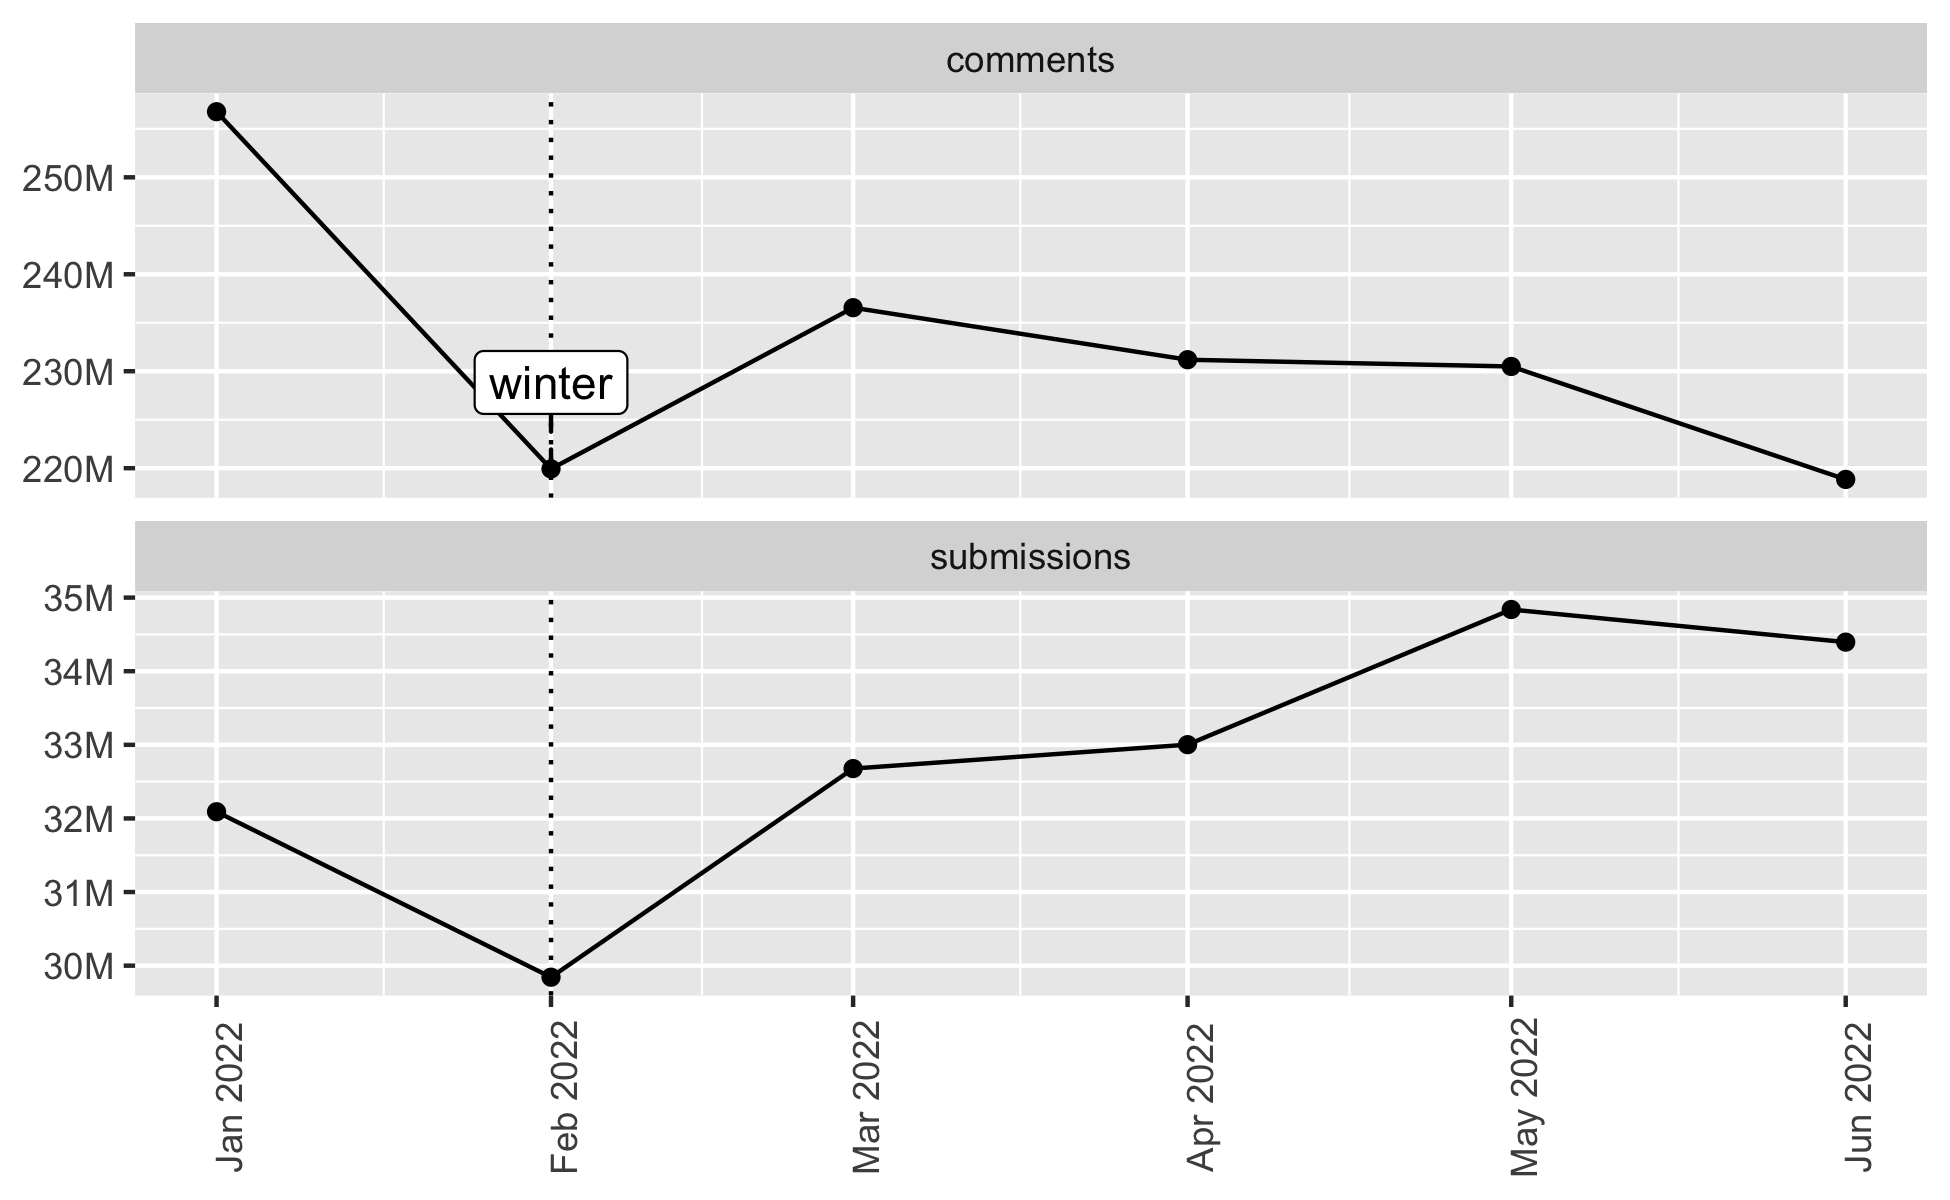
\includegraphics[width=\textwidth]{2022/count}
\caption{Comments and submissions}
\label{fig:count_2022}
\end{figure}

Figure \ref{fig:count_2022} displays comments and submissions by month.
The base dataset contains 1,590,619,\\748 items or 1,393,772,122 comments and 196,847,626 submissions by 31,323,324 unique users across 2,585,009 subreddits from January 2022 through June 2022.
The winter dip in activity is apparent as in previous chapters, however, unlike those chapters in which both comments and submissions remained level from March through June, there is a decrease in comments, this could be an outlier or Reddit reaching a ceiling.
We do not have a full three years of data to observe trends, we use the shorter six month scale to reduce processing time as the comments from January 2022 alone are over 333 GB uncompressed.
December 2017, the last month of data in Chapter 3, consists of 85,973,810 comments and 10,557,874 submissions compared to 256,766,675 comments and 32,091,070 submissions in January 2022, increases of 198.66\% and 203.95\%.
Similarly, from 2015 to 2017, there were just over 18.23 million unique users and 460,000 subreddits, Reddit saw continued massive growth through 2022.
Comments and submissions are again directly correlated, the ratio of submissions to comments is never lower than 12.5\% or higher than 15.72\%.

\begin{figure}[h]
\centering
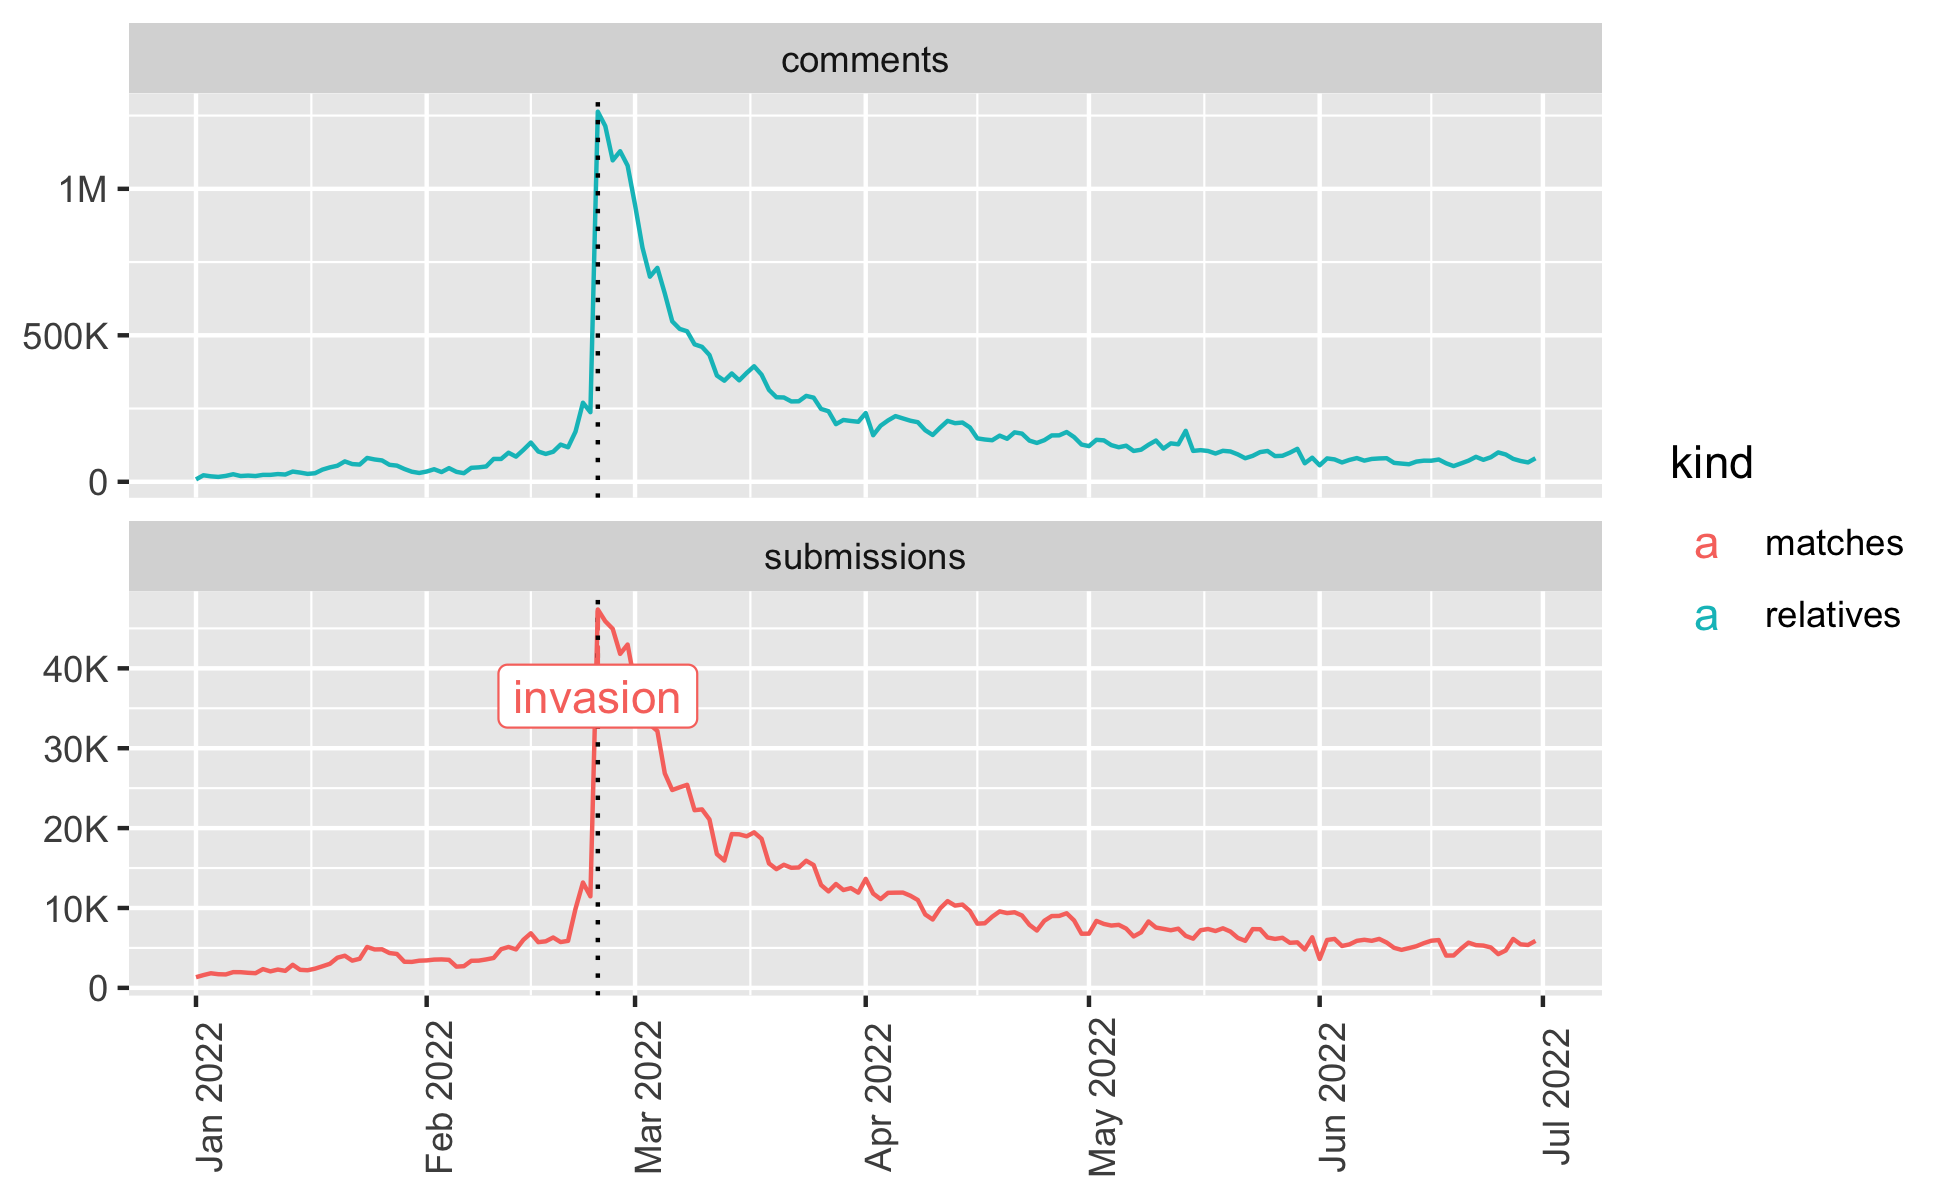
\includegraphics[width=\textwidth]{2022/match}
\caption{Matches and relatives}
\label{fig:matches_2022}
\end{figure}

Figure \ref{fig:matches_2022} displays matches and relatives by month.
Our selected six months of data are sufficient to capture the lead-up to the invasion of Ukraine which began on February 24 and the first few months of the conflict.
We want to reuse as much of Chapter 2 and 3 as possible, as such we use a slightly modified list of keywords from the Crimea data to filter out irrelevant items.
The item is considered a ``match'' (case-insensitive) if ``Euromaidan'', ``Donbas(s)'', ``Crimea'', ``Crimean(s)'', ``Putin'', ``Russia'', ``Russian(s)'', ``Ukraine'', ``Ukrainian(s)'', ``Zelensky(y)'', or ``Zelenskiy'' are found.
Once again, to reduce processing time, we only match against submissions and extract comments connected to them as relatives (there are no comment matches nor submission relatives).
On January 1, there are 1,334 submission matches and 8,065 comment relatives.
The peak is the day of the invasion with 47,365 submission matches and 1,263,243 comment relatives, activity then declines to 5,883 submissions and 80,249 comments on June 30.
In total there are 1,718,281 submission matches and 32,629,695 comment relatives across the six months.

\begin{table}[!ht]
\centering
\caption{Subreddits}
\begin{tabular}{lrrrrr}
\toprule
subreddit & \% & matches* & items & match \% & users \\
\midrule
worldnews             &   26.42 &   8643307 &    11747329 &    73.58 &   670840 \\
ukraine               &   10.39 &   3398449 &     4449535 &    76.38 &   226133 \\
UkrainianConflict     &    4.60 &   1504119 &     1765260 &    85.21 &   111672 \\
UkraineWarVideoReport &    3.46 &   1133154 &     1554034 &    72.92 &   125078 \\
CombatFootage         &    3.08 &   1007114 &     1543356 &    65.25 &   105349 \\
europe                &    2.22 &    725743 &     1857161 &    39.08 &    65027 \\
interestingasfuck     &    2.16 &    706541 &     4724053 &    14.96 &   218316 \\ß
news                  &    1.50 &    490912 &     5105814 &     9.61 &   102269 \\
politics              &    1.49 &    488251 &     6034055 &     8.09 &   111127 \\
AskARussian           &    1.46 &    476317 &      645065 &    73.84 &    25777 \\
conspiracy            &    1.40 &    458934 &     4302073 &    10.67 &    49986 \\
PublicFreakout        &    1.14 &    371466 &     5078293 &     7.31 &   106408 \\
neoliberal            &    1.09 &    355758 &     2846818 &    12.50 &    12885 \\
Damnthatsinteresting  &    1.06 &    348223 &     3066770 &    11.35 &   137484 \\
RussiaUkraineWar2022  &    0.82 &    269498 &      353670 &    76.20 &    35129 \\
ukpolitics            &    0.78 &    253829 &     1164034 &    21.81 &    10976 \\
NonCredibleDefense    &    0.69 &    226047 &      903671 &    25.01 &    21413 \\
nextfuckinglevel      &    0.65 &    211148 &     2937907 &     7.19 &    93475 \\
de                    &    0.62 &    201494 &     1500742 &    13.43 &    11344 \\
CryptoCurrency        &    0.55 &    181134 &     4980486 &     3.64 &    30981 \\
AskReddit             &    0.55 &    179205 &    39669986 &     0.45 &    56466 \\
ThatsInsane           &    0.51 &    168041 &     1069685 &    15.71 &    69375 \\
wallstreetbets        &    0.51 &    167041 &     7255226 &     2.30 &    46690 \\
Conservative          &    0.42 &    137499 &     1615715 &     8.51 &    19408 \\
CredibleDefense       &    0.34 &    112541 &      127050 &    88.58 &     6494 \\
russia                &    0.33 &    109417 &      171355 &    63.85 &    11906 \\
MapPorn               &    0.28 &     93019 &     1058404 &     8.79 &    32329 \\
canada                &    0.27 &     88474 &     1916732 &     4.62 &    16165 \\
CrazyFuckingVideos    &    0.26 &     85168 &     1691437 &     5.04 &    35943 \\
UkraineInvasionVideos &    0.26 &     84348 &      115132 &    73.26 &    13433 \\
summary (top 30)      &   69.32 &  22676191 &   121250848 &    32.64 &          \\
summary (all)         &  100.00 &  32713731 &  1456280549 &     0.49 &  2565090 \\
\bottomrule
\end{tabular}

\label{tab:subreddits_2022}
\end{table}

Table \ref{tab:subreddits_2022} displays the 30 subreddits with the most combined matches and relatives.
There are 32,713,731 matches and relatives by 2,565,090 unique users across 2,584,797 subreddits.
We exclude 212 subreddits, again mostly related to games, sports, language learning, or illicit material.
In comparison, there are around 1.56 million matches and relatives, 194,000 unique users, and 460,000 subreddits from 2013-2015 for Chapter 2 and 75.32 million items, 2.67 million users, and 70,000 subreddits from 2015-2017 for Chapter 3.
These 30 subreddits contain 69.32\% of all matches and relatives and these items are matched an average 32.64\% of the time, compared to the 0.49\% match rate average of all subreddits.
The top 5 subreddits include 47.95\% of all matches and relatives, have at least 1 million combined matches, more than 100,000 users, and match rates above 65\%.
The invasion is a popular topic across Reddit, but again, the top-heavy clustering of activity means that only  a limited number of subreddits would need to be targeted to reach a mass audience.
12 subreddits have a match rate above 25\%, 10 above 50\%, the subject dominating discussion there.
We note the 11th ranked subreddit r/conspiracy, found in the top 30 subreddits in every chapter.

\begin{table}[!ht]
\centering
\caption{Cites (matched and related items)}
\begin{tabular}{lrrrrrr}
\toprule
{} & \% & cites & users &  cites / & \% prog & \% cons \\
domain &  &  &  & users & users & users \\
\midrule
reddit.com*           &   21.94 &   2722645 &   630963 &         4.32 &         13.41 &          9.79 \\
youtube.com*          &    9.62 &   1193237 &   251651 &         4.74 &         16.49 &         17.00 \\
imgur.com             &    6.01 &    746031 &   200126 &         3.73 &         10.76 &          9.57 \\
wikipedia.org         &    3.70 &    459470 &   126526 &         3.63 &         19.83 &         11.21 \\
twitter.com*          &    3.45 &    428391 &    81020 &         5.29 &         23.65 &         22.73 \\
washingtonpost.com    &    2.03 &    252175 &    68845 &         3.66 &         40.00 &         19.00 \\
nytimes.com*          &    1.37 &    170305 &    54124 &         3.15 &         32.52 &         16.96 \\
cnn.com               &    1.13 &    139847 &    47536 &         2.94 &         36.94 &         22.44 \\
archive.org*          &    1.06 &    131008 &    20095 &         6.52 &         29.30 &         37.80 \\
google.com*           &    1.05 &    130314 &    48537 &         2.68 &         16.23 &          9.06 \\
politico.com          &    0.97 &    120307 &    37074 &         3.25 &         45.09 &         26.10 \\
thehill.com           &    0.90 &    111112 &    30702 &         3.62 &         43.44 &         28.39 \\
theguardian.com       &    0.84 &    103685 &    39020 &         2.66 &         41.09 &         17.61 \\
huffingtonpost.com*   &    0.72 &     89205 &    32861 &         2.71 &         44.03 &         18.67 \\
sli.mg                &    0.72 &     88865 &    15886 &         5.59 &         10.85 &         22.45 \\
independent.co.uk     &    0.62 &     77328 &    22716 &         3.40 &         44.67 &         13.21 \\
reuters.com           &    0.56 &     69324 &    23100 &         3.00 &         36.07 &         23.85 \\
wikileaks.org         &    0.52 &     64918 &    12213 &         5.32 &         19.71 &         23.63 \\
breitbart.com         &    0.50 &     62530 &    17220 &         3.63 &         25.17 &         52.35 \\
politifact.com        &    0.49 &     60982 &    26742 &         2.28 &         32.46 &         13.41 \\
foxnews.com           &    0.46 &     57092 &    23051 &         2.48 &         24.60 &         35.29 \\
bbc.com*              &    0.43 &     53800 &    24014 &         2.24 &         22.17 &         17.11 \\
businessinsider.com   &    0.41 &     51133 &    24106 &         2.12 &         34.92 &         21.58 \\
fivethirtyeight.com   &    0.38 &     47223 &    18570 &         2.54 &         39.89 &         11.51 \\
facebook.com*         &    0.37 &     46391 &    18790 &         2.47 &         18.70 &         10.88 \\
nbcnews.com           &    0.37 &     46260 &    19792 &         2.34 &         42.94 &         20.70 \\
realclearpolitics.com &    0.34 &     42197 &    15416 &         2.74 &         34.86 &         20.09 \\
theatlantic.com       &    0.34 &     41577 &    19370 &         2.15 &         44.51 &         17.66 \\
go.com                &    0.33 &     41301 &    17435 &         2.37 &         44.54 &         17.30 \\
npr.org               &    0.31 &     38915 &    18260 &         2.13 &         43.26 &         13.57 \\
summary (top 30)      &   61.96 &   7687568 &          &         3.32 &         31.07 &         20.03 \\
summary (all)         &  100.00 &  11761790 &  1174637 &         1.97 &         45.13 &         41.51 \\
\bottomrule
\end{tabular}

\label{tab:doms_2022}
\end{table}

\subsection{Classification}

To get a complete list of domains, we filter out 17 apparent bots, 9 domains, and combine link shorteners and domain aliases.
Table \ref{tab:doms_2022} displays the 30 most-cited domains within the matched and related items.
There are in total 3,853,869 cites by 494,105 unique users, these 30 domains are 69.02\% of these cites.
Yet again the same domains populate the top spots: reddit.com, youtube.com, imgur.com, wikipedia.org, and twitter.com are 57\% of cites (up from 44.72\% in the 2016 election), of the remaining sites only reuters.com, bbc.com, and theguardian.com are at least 1\%, this large set of domains is varied, widely-distributed, and mainstream.

Reddit domains are the most-cited: 1,303,651 times by 253,542 users, newsreadonline.com has the fewest users (44) out of the top 30 with 25,520 cites.
This supposedly Ukrainian source has a very inflated (580) cite per user ratio, suggesting bot activity.
It is the outlier in a list in which only twitter.com (7.4), www.gov.pl (10.07), medium.com (10.15), and webster.com (22.42) have cite to user ratios above 7.
Otherwise, this mix of domestic US, British, and Middle Eastern outlets represents a broad, organic view of the war, though we note the absence of Russian sources.

We reuse the domain lists established in the previous chapters to categorize users as Russian ($>$ 9 cites) and progressive and conservative users ($>$ 24 cites), which can overlap.
Notably, the Russian group is very small, with only archive.org over 10\% and 1.46\% of users overall in the top 30 domains.
Conservative users favor foxnews.com (64.03\% of cites), but Reddit's progressive tilt is apparent with 5 domains with greater than 20\% progressive users and 17 with more than 10\%.
None of the top 5 domains show group percentages higher than 5\%, and a number of domains, for example, t.me (Telegram) have low maximums (1.09\% progressive).
These user groups do not dominate as they did in previous chapters.

\begin{table}[!ht]
\centering
\caption{Wiki articles}
\begin{tabular}{lrrrr}
\toprule
{}                  & \% & cites & users & cites / \\
wikipedia.com/wiki/ &    &       &       & users   \\
\midrule
Azov\_Battalion                                     &    1.37 &    2675 &   1719 &         1.56 \\
Foundations\_Of\_Geopolitics                         &    0.95 &    1854 &    923 &         2.01 \\
Budapest\_Memorandum\_On\_Security\_Assurances         &    0.72 &    1409 &    978 &         1.44 \\
Holodomor                                          &    0.48 &     934 &    648 &         1.44 \\
List\_Of\_Foreign\_Aid\_To\_Ukraine\_During\_The\_Russo... &    0.47 &     923 &    489 &         1.89 \\
Russian\_Apartment\_Bombings                         &    0.41 &     795 &    527 &         1.51 \\
Whataboutism                                       &    0.38 &     746 &    493 &         1.51 \\
Kyivnotkiev                                        &    0.38 &     732 &    207 &         3.54 \\
2022\_Russian\_Invasion\_Of\_Ukraine                   &    0.30 &     582 &    375 &         1.55 \\
Wagner\_Group                                       &    0.29 &     563 &    385 &         1.46 \\
War\_In\_Donbas                                      &    0.23 &     457 &    336 &         1.36 \\
Dead\_Hand                                          &    0.21 &     418 &    298 &         1.40 \\
Stepan\_Bandera                                     &    0.20 &     383 &    247 &         1.55 \\
Russo-Ukrainian\_War                                &    0.19 &     364 &    284 &         1.28 \\
Winter\_War                                         &    0.19 &     363 &    292 &         1.24 \\
Dedovshchina                                       &    0.18 &     360 &    225 &         1.60 \\
Mutual\_Assured\_Destruction                         &    0.18 &     346 &    271 &         1.28 \\
Ukraine\%E2\%80\%93Nato\_Relations                     &    0.18 &     345 &    270 &         1.28 \\
Revolution\_Of\_Dignity                              &    0.17 &     330 &    243 &         1.36 \\
Battle\_Of\_Khasham                                  &    0.16 &     319 &    252 &         1.27 \\
Katyn\_Massacre                                     &    0.16 &     317 &    237 &         1.34 \\
Malaysia\_Airlines\_Flight\_17                        &    0.16 &     314 &    240 &         1.31 \\
United\_States\_Involvement\_In\_Regime\_Change         &    0.16 &     312 &    249 &         1.25 \\
Nato\_Bombing\_Of\_Yugoslavia                         &    0.16 &     310 &    224 &         1.38 \\
Stanislav\_Petrov                                   &    0.16 &     308 &    250 &         1.23 \\
Russian\_National\_Unity                             &    0.16 &     305 &    184 &         1.66 \\
Dmitry\_Utkin                                       &    0.15 &     302 &    187 &         1.61 \\
Annexation\_Of\_Crimea\_By\_The\_Russian\_Federation     &    0.15 &     296 &    243 &         1.22 \\
Russo-Georgian\_War                                 &    0.15 &     295 &    221 &         1.33 \\
Nuclear\_Weapons\_And\_Ukraine                        &    0.14 &     276 &    215 &         1.28 \\
summary (top 30)                                   &    9.19 &   17933 &        &         1.50 \\
summary (all)                                      &  100.00 &  195166 &  61887 &         1.16 \\
\bottomrule
\end{tabular}

\label{tab:wiki_2022}
\end{table}

Table \ref{tab:wiki_2022} displays the 30 most-cited Wikipedia articles, we do not include group percentages because none of the groups cite more than 2\% of these top articles.
There are 195,166 citations by 61,887 users, the top 30 are only 9.19\% of cites.
None of the articles has a cite per user ratio of higher than 3.54, indicating organic activity.
However, whataboutism and multiple articles from previous chapters return.
The Azov Battalion, Budapest, Holodomor, Stepan Bandera, annexation of Crimea, Russo-Georgian War, and nuclear weapons are among the 30 most-cited articles in Chapter 2 concerning Crimea.
The Revolution of Dignity in 2004 is a precursor to the revolution of 2014, the Katyn massacre echoes the massacre of Poles in Volhynia, both cited in Chapter 2, and while Flight 17 was not cited, it was a major topic.
Regime change by the United States is cited here, while in Chapter 2 covert regime change was highlighted, reflecting the secret and then overt actions of Russia in 2014 and 2022.

New articles include the Russian apartment bombings of 1999.
Over a span of 3 weeks, 5 bombings in Moscow and other cities killed more than 300 people, another three were prevented, local police arresting FSB agents for planting one set of explosives.
The attacks were blamed on Chechen extremists, Putin, prime minster at the time, was elected president and led the Second Chechen War that same year.
One conspiracy theory, with various individuals and organizations claiming evidence, suggests that Putin intentionally engineered these attacks to stay in and increase his power.
Alexander Litvinenko, former FSB agent, made this claim and was infamously assassinated by radioactive polonium in 2006.
The hardline Kadyrov family came into power as a result of the war in Chechnya, and the popularity of false flag claims in recent years may be a projection of these tactics.

The Wagner Group is a private paramilitary organization owned by ``Putin's chef'', Yevgeny Prigozhin.
Prigozhin was in Soviet prisons in the 1980s and began a catering and restaurant business in the 1990s during which time he came into Putin's orbit.
He founded the Internet Research Agency, featured in previous chapters and mentioned in the Mueller Report, a position that he admitted in February 2023, perhaps as part of a growing divide with the Kremlin.

Wagner has been involved in conflicts in Syria and Iraq, mercenaries coming into direct combat with US forces in 2018 in the Battle of Khasham, as well as Donbas and Africa.
The group is reportedly named after Hitler's favorite composer and run by Dmitry Utkin, a veteran of the wars in Chechnya with Nazi tattoos.
During the invasion of Ukraine, Wagner has been relied on heavily to limit conscription and public outrage, and began recruiting from Russian prisons.

Military culture is part of Russia's failure in the war, dedovshchina is the brutal hazing experienced by new recruits.
Putin has given multiple reasons for the invasion, including claims that Zelensky (Jewish) and his regime are nazis intent on destroying Russian culture (see Azov Battalion), but the primary motivating factor is probably NATO expansion into Eastern Europe.
Western involvement during the Balkan genocides of the late 1990s, particularly action against Serbia, Russia's old protectorate, is a point of contention.
Similarly, while the Bush administration and Putin courted each other before the invasion of Iraq in 2003, this conflict, a reminder of the Great Game between the British and Russian empires in the 19th century, in part motivated the Russian invasion of Georgia in 2008 and discussion of NATO membership for Ukraine, an apparent red line for Putin.

Finally, \emph{The Foundation of Geopolitics} was highly-cited by progressives in Chapter 3, during and following the 2016 presidential election.
The 1997 book, authored by ultranationalist Aleksandr Dugin, argues for a doctrine of Eurasianism which includes Russian annexation of Ukraine, expansion into Europe and the Middle East, and the forming of relationships with traditional enemies of the United States including Iran.
The book supposedly has had some influence within the Russian military and is at times described by westerners as a roadmap and guide to actions including Putin's invasion of Ukraine.
This in itself is a kind of conspiracy theory, Dugin's occult, neofascist influences are an attractive target, but many of his prescriptions are actions any leader seeking to restore Russia to Soviet or imperial power would naturally take.
Reddit's discussion of it at times sounds like that surrounding the likely fake Tanaka war memo preceding World War II, discussed in the introduction.
It is difficult to say to what extent it has influenced the thinking of Russian leadership.
Nevertheless, in August 2022, his daughter Darya Dugina, also a nationalist, was killed in a car bombing outside of Moscow.
Whether this was the work of Russians against the war, Ukrainian special forces, out lash by the regime for a lagging conflict, or a false flag intended to stir Russian nationalism is unclear. 

\begin{table}[h!]
\centering
\caption{User groups}
\begin{tabular}{lrrrrr}
\toprule
{}    & users & change & doms & comment   & submission \\
group &       &        &      & relatives & matches    \\
\midrule
   conservative &        98 &   -2339 &   116400 &              23021 &               98105 \\
   progressive &       141 &   -4234 &   254280 &              63434 &              111227 \\
    rus &        66 &    -271 &    48959 &              19607 &               37993 \\
 totals &  32193996 &        &  5311670 &           32629695 &             1718281 \\
\bottomrule
\end{tabular}

\label{tab:groups_2022}
\end{table}

Table \ref{tab:groups_2022} displays basic stats about the groups: the number of users within, how many domains they post, and the quantity of submission matches and comment relatives.
Compared to Chapter 2, there are 271 fewer users that post at least 10 rus domains and compared to Chapter 3, there are 2,399 fewer conservative and 4,234 fewer progressive users with at least 25 cites.
This results in a corresponding drop in posted material: there are 39.72\% rus, 5.60\% conservative, and 8.95\% progressive domains posted by each group compared to the previous chapters.
Rus users post 28.47\%, conservative users 1.1\%, and progressive users 1.55\% of comment relatives, and conservative users 12.42\% and progressive users 11.83\% of submission matches.
Curiously, rus users post 117.66\% of submission matches despite their smaller population numbers, suggesting bots.
What explains this reduced activity?
Reddit is likely monitoring and restricting artificial user behavior better than previously, especially with the revelations of the Mueller Report, and user activity itself has probably adapted.
We discuss this further in the chapter conclusion.

\subsection{Network Analysis}

\begin{figure}[!ht]
\centering
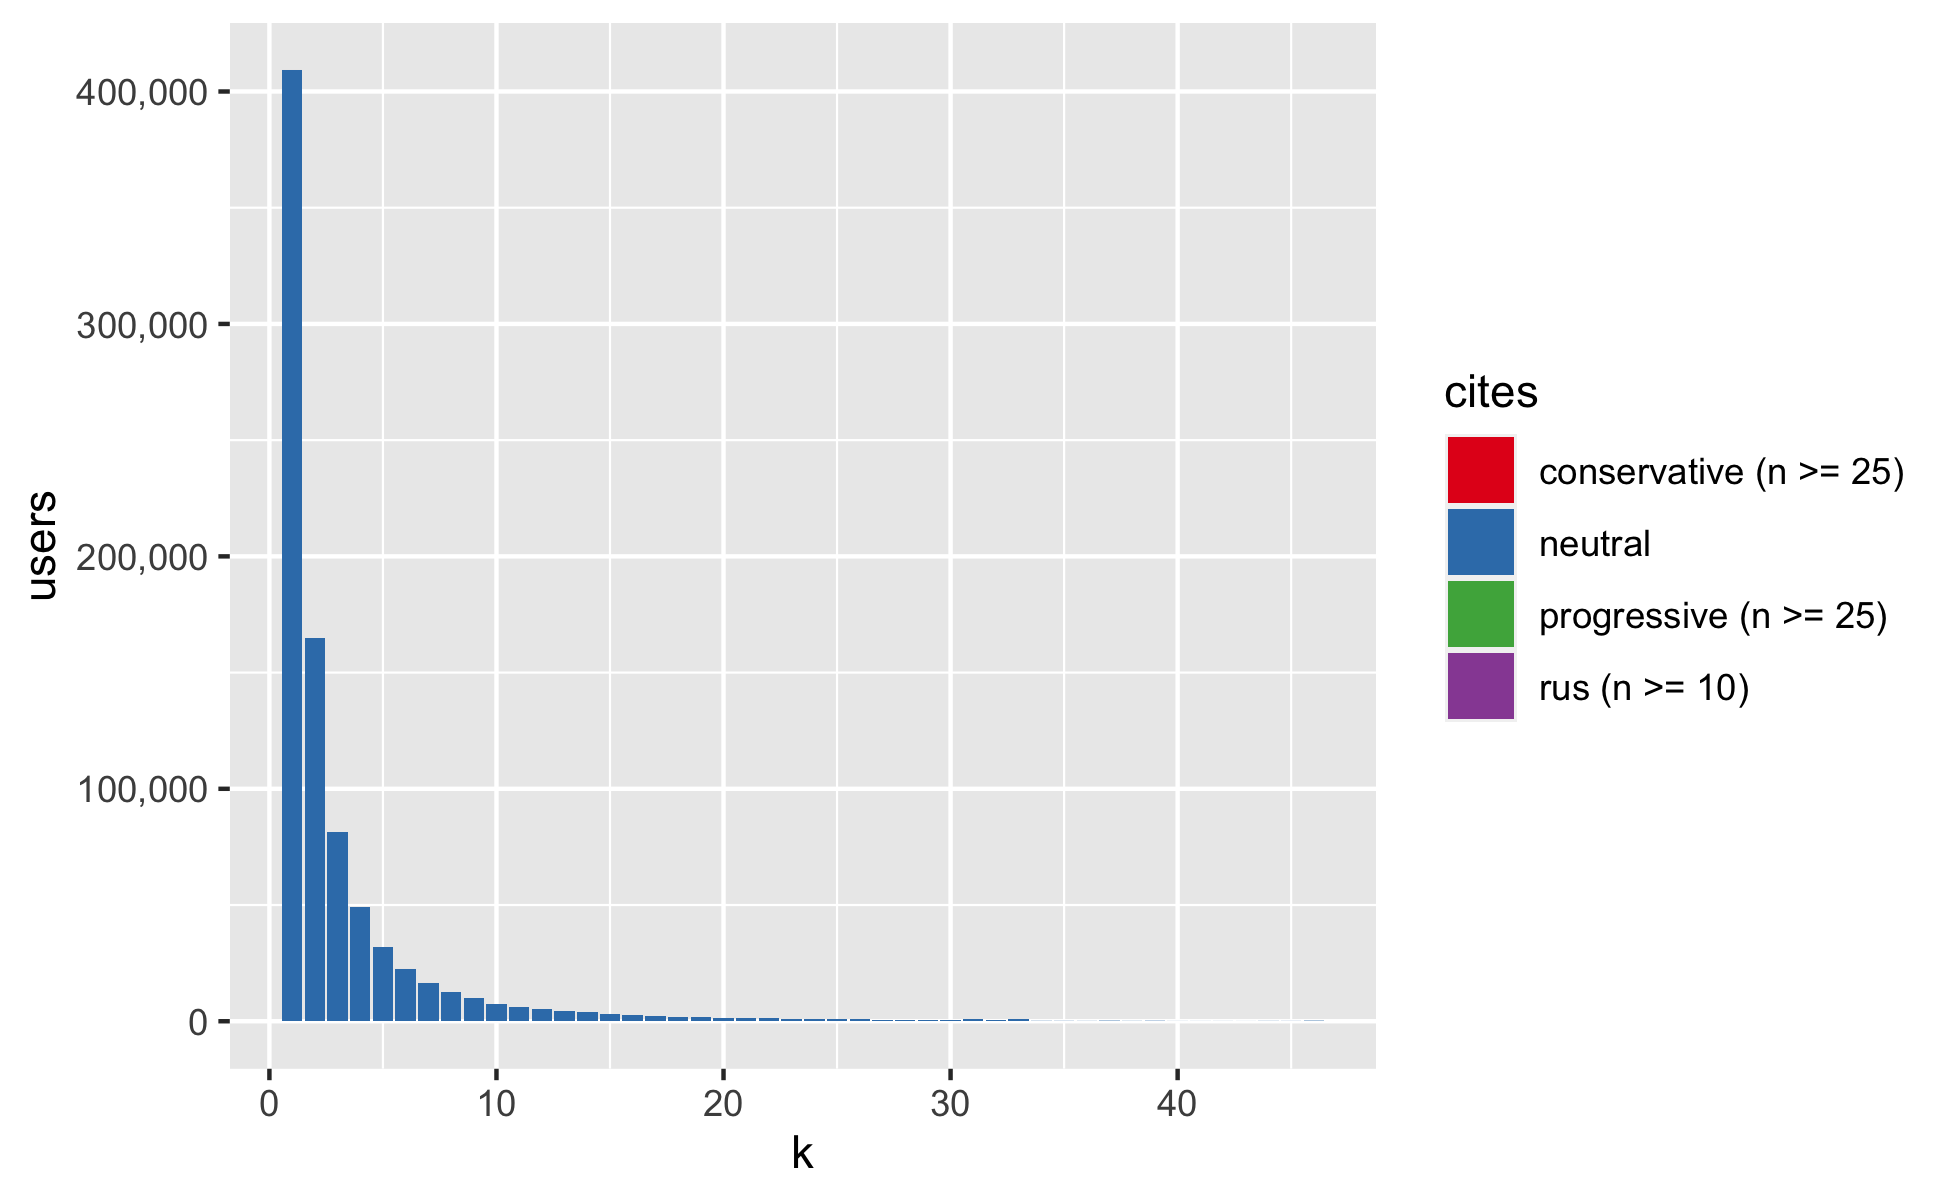
\includegraphics[width=\textwidth]{2022/kshells}
\caption{K-shells}
\label{fig:kshells_2022}
\end{figure}

Figure \ref{fig:kshells_2022} displays the k-core distribution.
The largest-connected component of the user network is composed of 850,529 users.
Neutral users have an extreme skew to the right with 805,437 (94.72\%) users located in the first 10 shells (on the periphery).
There are 46 shells compared to 31 in Chapter 2 and 94 in Chapter 3, which makes sense as k-cores are by number of connections, the more users, the more connections and shells.
Previously, we displayed this distribution by the percent of users from each group.
This is unnecessary here, while we still show user groups, none of the rus, conservative, or progressive groups have more than 6 users per shell.
Similarly, they do not cluster in the highest shells as seen earlier, they do not dominate discussion.

\begin{table}[!ht]
\footnotesize
\centering
\caption{Most ties in top k-shell}
\begin{tabular}{lrrrlrlr}
\toprule
{} & ties & prog & cons & subreddit & cites & dom & cites \\
user &    & cites & cites &         & in    &     & of    \\
\midrule
spsteve             &  1452 &           3 &           0 &    worldnews &       610 &      twitter.com &       466 \\
nohbody123          &  1236 &          11 &           1 &    worldnews &       701 &      twitter.com &       350 \\
catsinbananahats    &  1232 &           2 &           1 &  AskARussian &        23 &       reddit.com &        57 \\
BlatantConservative &  1098 &           4 &           0 &    worldnews &       296 &       reddit.com &       140 \\
Torifyme12          &   990 &           1 &           2 &    worldnews &       117 &      twitter.com &        33 \\
imyourforte         &   988 &           2 &           4 &    worldnews &       778 &    liveuamap.com &       298 \\
InnocentTailor      &   975 &           2 &           0 &    worldnews &       320 &    wikipedia.org &       106 \\
thrae\_awa           &   904 &           4 &           2 &    worldnews &       901 &      twitter.com &       515 \\
LaughingChimera1    &   881 &          10 &           3 &    worldnews &      1016 &      twitter.com &       464 \\
Recidiva            &   868 &           5 &           1 &    worldnews &        96 &    wikipedia.org &        12 \\
mewehesheflee       &   861 &          12 &           1 &    worldnews &       273 &    wikipedia.org &        62 \\
TintedApostle       &   821 &          27 &           8 &    worldnews &       330 &      youtube.com &        81 \\
Wolverinexo         &   821 &           0 &           0 &    worldnews &        26 &    wikipedia.org &        14 \\
haavarl             &   772 &           6 &           1 &    worldnews &       713 &      twitter.com &       382 \\
slothsan            &   757 &           1 &           0 &    worldnews &        88 &      twitter.com &        29 \\
dockneel            &   735 &          86 &           0 &    worldnews &       200 &  theatlantic.com &        86 \\
etzel1200           &   731 &           0 &           2 &    worldnews &       290 &      twitter.com &       180 \\
helm                &   729 &           2 &           0 &    worldnews &        56 &      twitter.com &        14 \\
rishcast            &   709 &          15 &          10 &    worldnews &      1131 &      twitter.com &      1399 \\
TLJDidNothingWrong  &   678 &           7 &           0 &    worldnews &       247 &      twitter.com &       123 \\
Papaofmonsters      &   677 &           0 &           0 &    worldnews &        27 &    wikipedia.org &        19 \\
acox199318          &   674 &           0 &           2 &    worldnews &         8 &      twitter.com &         5 \\
psychoCMYK          &   670 &           6 &           1 &    worldnews &      1025 &    wikipedia.org &       260 \\
oxpoleon            &   653 &           0 &           0 &    worldnews &        58 &    wikipedia.org &        22 \\
SefferWeffers       &   641 &           1 &           1 &    worldnews &        90 &      twitter.com &        22 \\
stirly80            &   641 &           7 &           3 &    worldnews &      2344 &      twitter.com &      1224 \\
yes\_its\_him         &   632 &          10 &           6 &    worldnews &       338 &    wikipedia.org &        60 \\
xmuskorx            &   629 &           2 &           1 &    worldnews &       176 &    wikipedia.org &        81 \\
mbattagl            &   616 &           0 &           0 &    worldnews &        18 &       reddit.com &         7 \\
dianaprd            &   615 &           9 &           0 &    worldnews &       414 &    pravda.com.ua &       151 \\
\bottomrule
\end{tabular}

\label{tab:topk_2022}
\end{table}

Table \ref{tab:topk_2022} displays stats about the 30 users with the most ties (responses) to other users in the top k-shell.
Rus cites are not displayed, none of these users have more than 2.
Two users are classified as progressive with at least 25 cites (u/TintedApostle and u/dockneel), all of the latter's progressive cites (86) are from theatlantic.com.
No users are classified as conservative, u/rishcast has the most (10), but has more progressive cites.
Only a single user does not post links most often in r/worldnews: 4 have more than 1,000 cites, 9 have more than 500, and 20 have more than 100 there.
14 users cite Twitter most often, 2 more than 1,000 times, 9 more than 100 times.
9 users cite Wikipedia most often, 3 Reddit, and 1 Ukraine's Pravda, the latter worth nothing because the country was part of the same propaganda system as Russia in the USSR.
That these prolific posters have the most ties is not surprising, but these numbers emphasize how much social media drives coverage and awareness of events.

\begin{table}[!ht]
\centering
\scriptsize
\caption{Users by betweenness centrality}
\begin{tabular}{lrrrrrll}
\toprule
{}   & bet    & in    & out   & prog  & cons  & dom & subreddit \\
user & cent z & deg z & deg z & cites & cites &      &          \\
\midrule
UkraineWithoutTheBot &      319.87 &    130.12 &       9.45 &           0 &           0 &    webster.com &  UkraineWarVideoReport \\
catsinbananahats     &      105.29 &     32.05 &      12.06 &           2 &           1 &     reddit.com &            AskARussian \\
crimeo               &       85.02 &     15.37 &       1.20 &           4 &           0 &  wikipedia.org &              worldnews \\
Cloaked42m           &       82.27 &     25.15 &       2.93 &           0 &           0 &  wikipedia.org &              worldnews \\
panzerfan            &       76.64 &     23.39 &      43.21 &          10 &           5 &    twitter.com &                ukraine \\
spsteve              &       75.12 &     50.25 &       8.82 &           3 &           0 &    twitter.com &              worldnews \\
Prunestand           &       72.85 &     16.62 &      83.09 &         116 &          12 &        bbc.com &      UkrainianConflict \\
AlwaysBlamesCanada   &       72.83 &      8.91 &       1.21 &           0 &           0 &     reddit.com &          CombatFootage \\
Jealous\_Tangerine\_93 &       71.06 &     35.50 &       3.21 &           0 &           2 &     reddit.com &     RussainCrimialActs \\
3BM15                &       69.95 &     27.85 &      17.91 &          10 &           1 &    twitter.com &           warinukraine \\
Geaux2020            &       64.79 &     20.02 &       3.73 &           0 &           1 &  wikipedia.org &              worldnews \\
InnocentTailor       &       64.58 &     49.07 &       5.76 &           2 &           0 &  wikipedia.org &              worldnews \\
DMBFFF               &       61.85 &     22.81 &       3.85 &          29 &           0 &  wikipedia.org &      UkrainianConflict \\
Greybatclone         &       61.66 &     25.36 &       2.79 &           1 &           0 &     reddit.com &      UkrainianConflict \\
Vegetaman916         &       60.40 &     14.22 &       3.92 &           8 &           1 &       youtu.be &               collapse \\
Haunting\_Pay\_2888    &       60.11 &     63.29 &       6.96 &           1 &           0 &       youtu.be &      UkrainianConflict \\
Ok\_Pomelo7511        &       60.05 &     24.84 &       5.19 &           0 &           0 &     reddit.com &            AskARussian \\
Easy-Smoke1467       &       58.33 &     36.72 &      10.57 &           2 &           0 &     reddit.com &  UkraineWarVideoReport \\
SiarX                &       56.48 &     18.44 &       2.38 &           0 &           0 &  wikipedia.org &              worldnews \\
BrainBlowX           &       55.96 &     22.15 &       2.12 &           0 &           0 &       youtu.be &      UkrainianConflict \\
Nutsband\_Handi       &       55.47 &     22.39 &       3.91 &           5 &           8 &    twitter.com &  UkraineWarVideoReport \\
PolecatXOXO          &       55.15 &     48.41 &       7.44 &           1 &           0 &  wikipedia.org &                ukraine \\
punkish138           &       54.55 &     12.35 &       1.15 &           0 &           0 &     reddit.com &              worldnews \\
Torifyme12           &       52.40 &     48.97 &       7.14 &           1 &           2 &    twitter.com &              worldnews \\
Elocai               &       52.02 &     34.59 &       2.24 &           0 &           0 &     reddit.com &              worldnews \\
Ridley\_Rohan         &       51.78 &      7.69 &       1.32 &           0 &           0 &    youtube.com &                chomsky \\
RedditIsAJoke69      &       51.15 &      8.87 &       1.55 &           0 &           0 &    youtube.com &             conspiracy \\
HostileRespite       &       51.06 &     15.32 &       2.21 &           0 &           0 &    youtube.com &                ukraine \\
Floofyboy            &       50.84 &     11.61 &       3.89 &           0 &           2 &    twitter.com &              worldnews \\
Disastrous\_Tip\_3347  &       50.78 &     14.14 &       2.46 &           0 &           0 &     reddit.com &                 europe \\
\bottomrule
\end{tabular}

\label{tab:bet_cent_2022}
\end{table}

Table \ref{tab:bet_cent_2022} displays the 30 users with the highest betweenness centrality in terms of z-score.
Betweenness centrality is a measure of how often a user is on the shortest path connecting other users, z-scores are the number of standard deviations from the mean, u/UkraineWithoutTheBot has a betweenness centrality 319.87 standard deviations from the mean.
These users are interacting with users that in turn are interacting with many others, their high in and out-degrees similarly show them responding and being responded to more than the average user.
None of the users is classified as rus with at least 10 cites, u/3BM15 has the most with 7.
There are two users classified as progressive (u/Prunestand and u/DMBFFF), the former also has the most conservative cites (12) and no users are classified as conservative.
There is a wider mix of domains, though Reddit (9), Wikipedia (7), Twitter (6), and YouTube (6) are still preferred by many users.
Subreddits too are more diverse with r/worldnews (10), r/UkrainianConflict (5), r/ukraine (4), and r/UkraineWarVideoReport (3) popular and r/conspiracy making another appearance.

\begin{table}[!ht]
\centering
\scriptsize
\caption{Users by total degree}
\begin{tabular}{lrrrrrll}
\toprule
{}   & tot   & in  & out & prog  & cons  & dom & subreddit \\
user & deg z & deg & deg & cites & cites &     &           \\
\midrule
WorldNewsMods     &     615.85 &       5 &   289135 &           0 &           0 &           reddit.com &             worldnews \\
manticor225       &     178.94 &     206 &    83847 &           0 &           0 &          reuters.com &             worldnews \\
progress18        &     111.48 &     101 &    52288 &           9 &           0 &          twitter.com &             worldnews \\
DoremusJessup     &     105.74 &      14 &    49680 &           2 &           0 &         france24.com &             worldnews \\
SmokeSinseLoud    &     100.33 &     481 &    46670 &           0 &           0 &              redd.it &  RussiaUkraineWar2022 \\
QuirkyQuarQ       &      98.34 &    1232 &    44989 &          18 &           4 &          twitter.com &             worldnews \\
dieyoufool3       &      97.00 &     231 &    45357 &           0 &           0 &           reddit.com &             worldnews \\
TheRealMykola     &      94.42 &    2465 &    41915 &           7 &           3 &           reddit.com &               ukraine \\
IneptProfessional &      93.83 &    1282 &    42822 &          12 &           7 &          twitter.com &     UkrainianConflict \\
Prunestand        &      82.05 &    1574 &    36998 &         116 &          12 &              bbc.com &     UkrainianConflict \\
samplestiltskin\_  &      77.75 &      42 &    36510 &           0 &           0 &  businessinsider.com &             worldnews \\
admirablegoma     &      77.18 &       6 &    36281 &           0 &           0 &          reuters.com &             worldnews \\
Paneraiguy1       &      73.47 &     187 &    34359 &           3 &           2 &  businessinsider.com &             worldnews \\
ukpolbot          &      73.36 &      62 &    34430 &           0 &           0 &           reddit.com &            ukpolitics \\
JihadMeAtHello    &      73.36 &      61 &    34430 &           3 &           2 &          reuters.com &             worldnews \\
valuingvulturefix &      73.24 &      11 &    34428 &           0 &           0 &           reddit.com &             worldnews \\
nOMnOMShanti      &      70.85 &     493 &    32824 &           5 &           0 &             youtu.be &               ukraine \\
Isentrope         &      68.99 &     249 &    32193 &           0 &           0 &          twitter.com &             worldnews \\
molokoplus359     &      63.20 &    1253 &    28473 &          12 &          12 &          twitter.com &                europe \\
PanEuropeanism    &      59.59 &     437 &    27594 &          18 &           5 &          twitter.com &                europe \\
rishcast          &      59.44 &    1495 &    26462 &          15 &          10 &          twitter.com &             worldnews \\
a1b0r             &      58.14 &     154 &    27194 &           1 &           4 &              redd.it &         ArtForUkraine \\
irishrugby2015    &      57.28 &    1075 &    25869 &           6 &           5 &          twitter.com &           ThatsInsane \\
RallyToTheColors  &      56.78 &     932 &    25780 &           3 &           0 &              redd.it &               ukraine \\
lonely\_fucker69   &      56.54 &      32 &    26566 &           0 &           0 &              redd.it &     interestingasfuck \\
vancouver\_reader  &      56.34 &      74 &    26429 &          64 &           7 &               cbc.ca &     UkrainianConflict \\
CapitalString     &      55.94 &    1046 &    25271 &           5 &           6 &           reddit.com &               ukraine \\
jesterboyd        &      55.55 &     922 &    25210 &           0 &           0 &           reddit.com &               ukraine \\
PeasKhichra       &      54.72 &      13 &    25730 &           0 &           0 &              redd.it &     interestingasfuck \\
one\_and\_equal     &      52.33 &     262 &    24362 &           5 &           4 &           censor.net &     UkrainianConflict \\
\bottomrule
\end{tabular}

\label{tab:tot_deg_2022}
\end{table}

Finally, Table \ref{tab:tot_deg_2022} displays the 30 users with the highest combined in and out-degrees.
Several users are found in the previous two tables, all of the users here have at least 24,000 outgoing connections to other users, which explains their high placement.
However, 8 users have at least 1,000 incoming connections which means they are not just spammers that are being ignored.
None of these users have more than 2 rus cites, two (u/Prunestand and u/vancouver\_reader) are classified as progressive, the former once again has the most conservative cites with 12.
While there are more conservative cites, none of these users meets the threshold to be grouped as such.
The same domains: Reddit (12), Twitter (8), subreddits: r/worldnews (13), r/UkrainianConflict (4), and r/ukraine (5) dominate, which reiterates importance of social media and the ability to target the majority of users using a few selected subreddits.
We also observe that the user with by far the highest total degree is an apparent moderator, u/WorldNewsMods, as in the previous chapter with u/maxwellhill, these users have untold anonymous power to direct discourse.

\subsection{Textual Analysis}

Next, we train a Word2vec model on submissions and comments and display it as graph of talking points.
Unlike the previous chapters, because we do not have substantial groups of users, we do not train separate models for each group.
We use t-SNE to convert the high-dimension vectors into two dimensions and k-means to identify clusters of terms.
There is no optimal way of presenting dimensionality-reduction nor clustering, we are only viewing a slice of the data, but the graphs do have face-validity.
Terms in the context of Word2vec are italicized going forward. 

\begin{figure}[!ht]
\centering
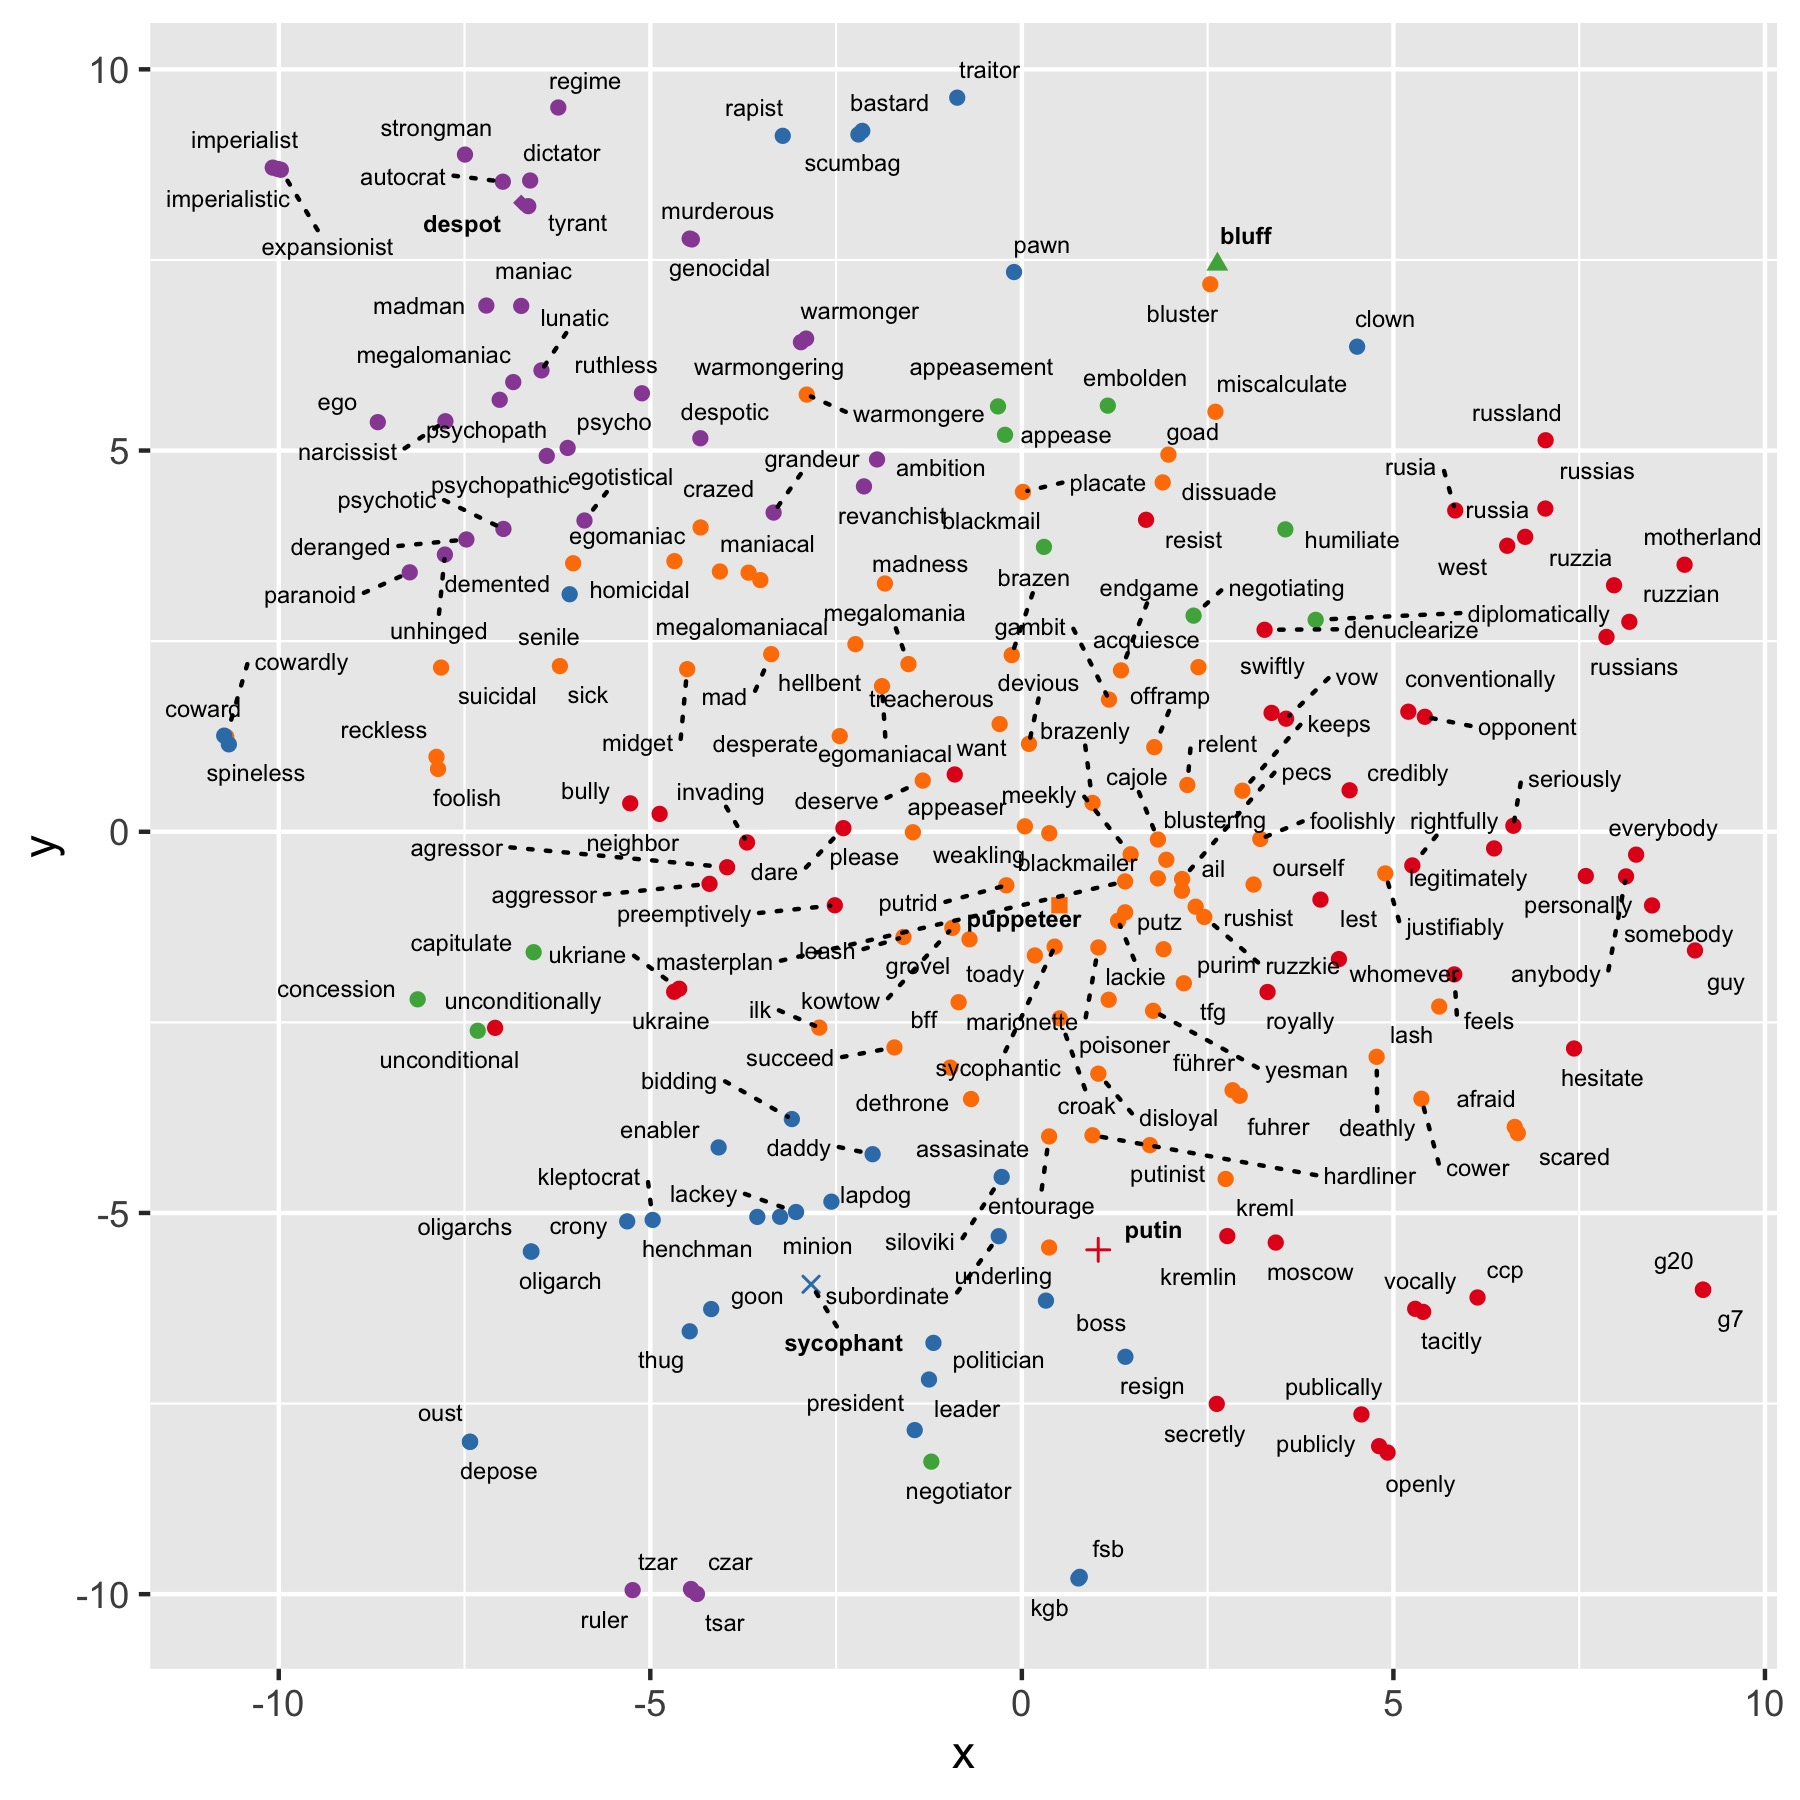
\includegraphics[width=\textwidth]{2022/putin}
\caption{Most-similar to ``putin''}
\label{fig:putin_2022}
\end{figure}

Figure \ref{fig:putin_2022} displays the 217 most-similar terms to ``putin'' with 183 excluded.
Individuals are removed in order to avoid cross-cutting clustering across people and things, several non-grammatical terms due to bad word splits have been filtered out as well, but the largest number of exclusions are derogatory monikers for Putin.
Compared to figures \ref{fig:superspreader_putin} and \ref{fig:neutral_putin} in Chapter 2, this figure is almost entirely negative.

We locate \emph{putin} at the bottom-center of the graph in a cluster of entities connected to and competing with him: \emph{kremlin, ruzzia(n), russia(s), west, motherland, moscow, opponent, ukraine, ukriane, ccp, russland, g7, rusia, neighbor, g20, russians}.
Nearby, in the bottom-left is the \emph{sycophant} cluster of individuals that work underneath him: \emph{crony, lackey, lapdog, henchman, depose, siloviki, sycophant, minion, kleptocrat, oust, daddy, coward, oligarch(s), clown, senile, thug, goon, enabler, bidding, scumbag, resign, politician, boss, bastard, pawn, spineless, fsb, kgb, traitor, subordinate}.

The \emph{puppeteer} cluster at the center of the graph includes a mix of terms related to both Putin and his followers: \emph{underling, entourage, grovel, appeaser, please, toady, cowardly, kreml, cower, hardliner, putrid, ruzzkie, foolishly, dethrone, yesman, kowtow, lackie, bff, weakling, afraid, rushist, ilk, leash, fuhrer, assasinate, lash, putz, poisoner, sycophantic, blackmailer, scared, führer, deathly, masterplan, putinist, meekly, croak, blustering, marionette, disloyal, ail}.
This blends into the \emph{bluff} cluster towards the top of the graph with a discussion of tactics: \emph{acquiesce, miscalculate, placate, relent, goad, offramp, brazen(ly), cajole, endgame, dissuade, gambit}, and the \emph{despot} cluster to the top-left with descriptions of Putin's pyschological makeup: \emph{egomaniac(al), maniacal, megalomania(cal), warmongere, desperate, demented, homicidal, crazed, hellbent, foolish, reckless, madness, suicidal, midget, sick, treacherous, devious}.

In the top-center of thee graph is the aforementioned \emph{bluff} cluster with reactions to him: \emph{embolden, humiliate, appease(ment), capitulate, diplomatically, blackmail, unconditional, negotiator, negotiating, concession}.
Finally, the \emph{despot} grouping at the top-left contains the most negative descriptors: \emph{dictator, autocrat, despotic, madman, maniac, tyrant, megalomaniac, strongman, warmonger(ing), murderous, regime, tzar, ego(tistical), psycho(path), lunatic, czar, expansionist, paranoid, imperialistic, psychopathic, genocidal, revanchist, ambition, tsar, ruthless, deranged, unhinged, psychotic, imperialist, narcissist, ruler, grandeur}.

\begin{figure}[!ht]
\centering
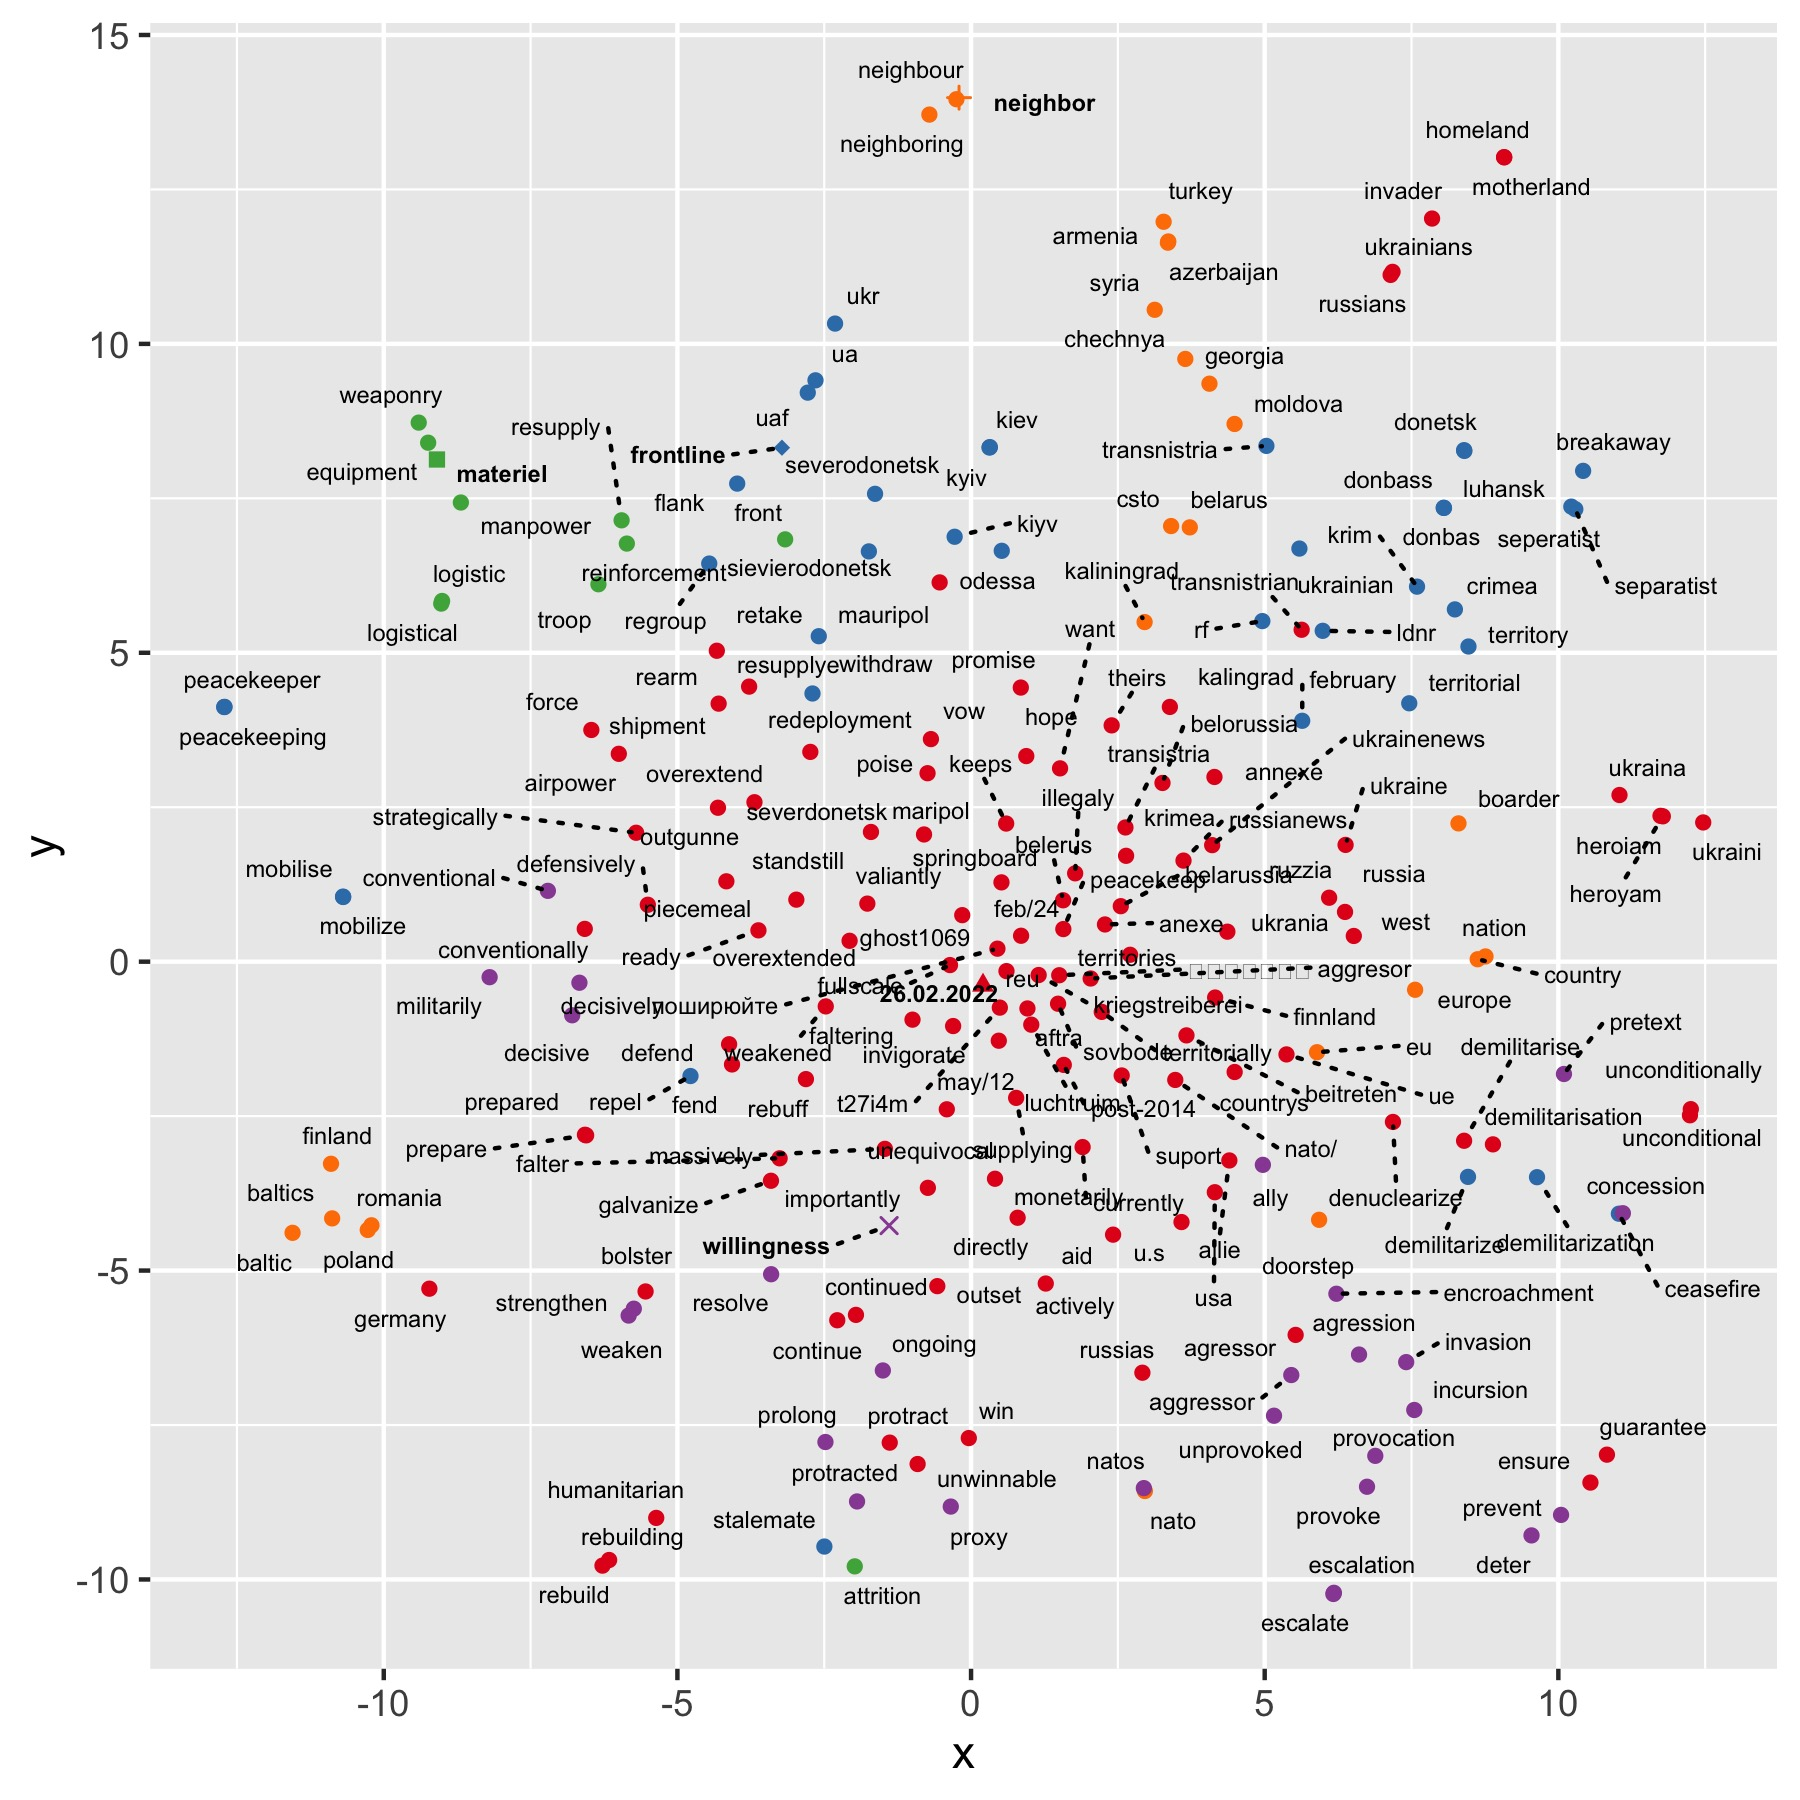
\includegraphics[width=\textwidth]{2022/ukraine}
\caption{Most-similar to ``ukraine''}
\label{fig:ukraine_2022}
\end{figure}

We plotted talking points for ``crimea'' in Chapter 2, now we adjust and compare to the larger topic.
Figure \ref{fig:ukraine_2022} displays the 222 most-similar terms to ``ukraine'' with 78 excluded.
Our graph is oriented around a central \emph{26.02.2022} cluster of terms related to the war.
Towards the top is the \emph{frontline} cluster with an emphasis on the conflict in the east: \emph{donbas(s), ua, crimea, ukr(ainian), transnistria, territory, kyiv, krim, uaf, separatist, regroup, kiev, demilitarize, stalemate, territorial, peacekeeper, ldnr, mobilise, seperatist, luhansk, odessa, mobilize, repel, ceasefire, flank, rf, demilitarization, sievierodonetsk, severodonetsk, peacekeeping, withdraw, breakaway, february, retake, kiyv, donetsk}.
We note the multiple spellings, suggesting a global audience as well as one less familiar with the topics under discussion.

The top-left includes the \emph{materiel} grouping concerned with logistics: \emph{reinforcement, materiel, troop, front, attrition, resupply, weaponry, manpower, logistic(al), equipment}.
This bleeds over into the central cluster: \emph{piecemeal, standstill, defensively, outgunne, shipment, rearm, resupplye, force, ready, overextend(ed), airpower, redeployment}.
Below \emph{materiel} and wrapping around the bottom of the graph is the \emph{willingness} group of more abstract needs and issues: \emph{aggressor, militarily, prolong, decisive(ly), weaken, ally, deter, proxy, pretext, natos, unprovoked, protracted, ongoing, conventional, escalate, invasion, prevent, encroachment, strengthen, resolve, provoke, provocation, concession, escalation, incursion, agression}.
Once again the central cluster contains similar terms: \emph{continue(d), agressor, conventionally, demilitarise, (de)fend, bolster, prepare(d), invader, rebuff, standstill, defensively, massively, unconditional(ly), aggresor, falter, demilitarisation, vow, suport, currently, win, unequivocal, unwinnable, supplying, guarantee, monetarily, weakened, humanitarian, faltering, rebuild(ing), defend, protract, galvanize, redeployment, valiantly, actively, importantly, ensure, strategically, invigorate, aid}.

Next, \emph{neighbor} cluster at the top, bottom-left, and right includes various surrounding countries and regions: \emph{belarus, europe, moldova, nato, country, poland, kaliningrad, nation, azerbaijan, finland, syria, georgia, eu, armenia, neighbour, baltics, romania, boarder, baltic, doorstep, neighboring, chechnya, csto, turkey}.
Related topics from the core cluster are: \emph{ukraine, russia(s), ukrainians, ukrania, ruzzia, west, ukraina, transistria, russians, kalingrad, belarussia, homeland, krimea, transnistrian, mauripol, maripol, ue, u.s, force, belerus, belorussia, motherland, usa, allie, ukraini, germany, countrys, finnland}.
We again note the variety of spellings.

Some of the topics from the middle group worth highlighting: \emph{kriegstreiberei, ghost1069, may/12, heroyam, beitreten, ukrainenews, heroiam, luchtruim, russianews, feb/24}.
Discussion occurred in a variety of languages, we only pick up traces of this.
\emph{ghost1069} might refer to a case of Ukrainian propaganda from the early days of the war, the ``Ghost of Kyiv'', an Ukrainian fighter pilot with multiple kills \cite{bubola2022}.

\begin{figure}[!ht]
\centering
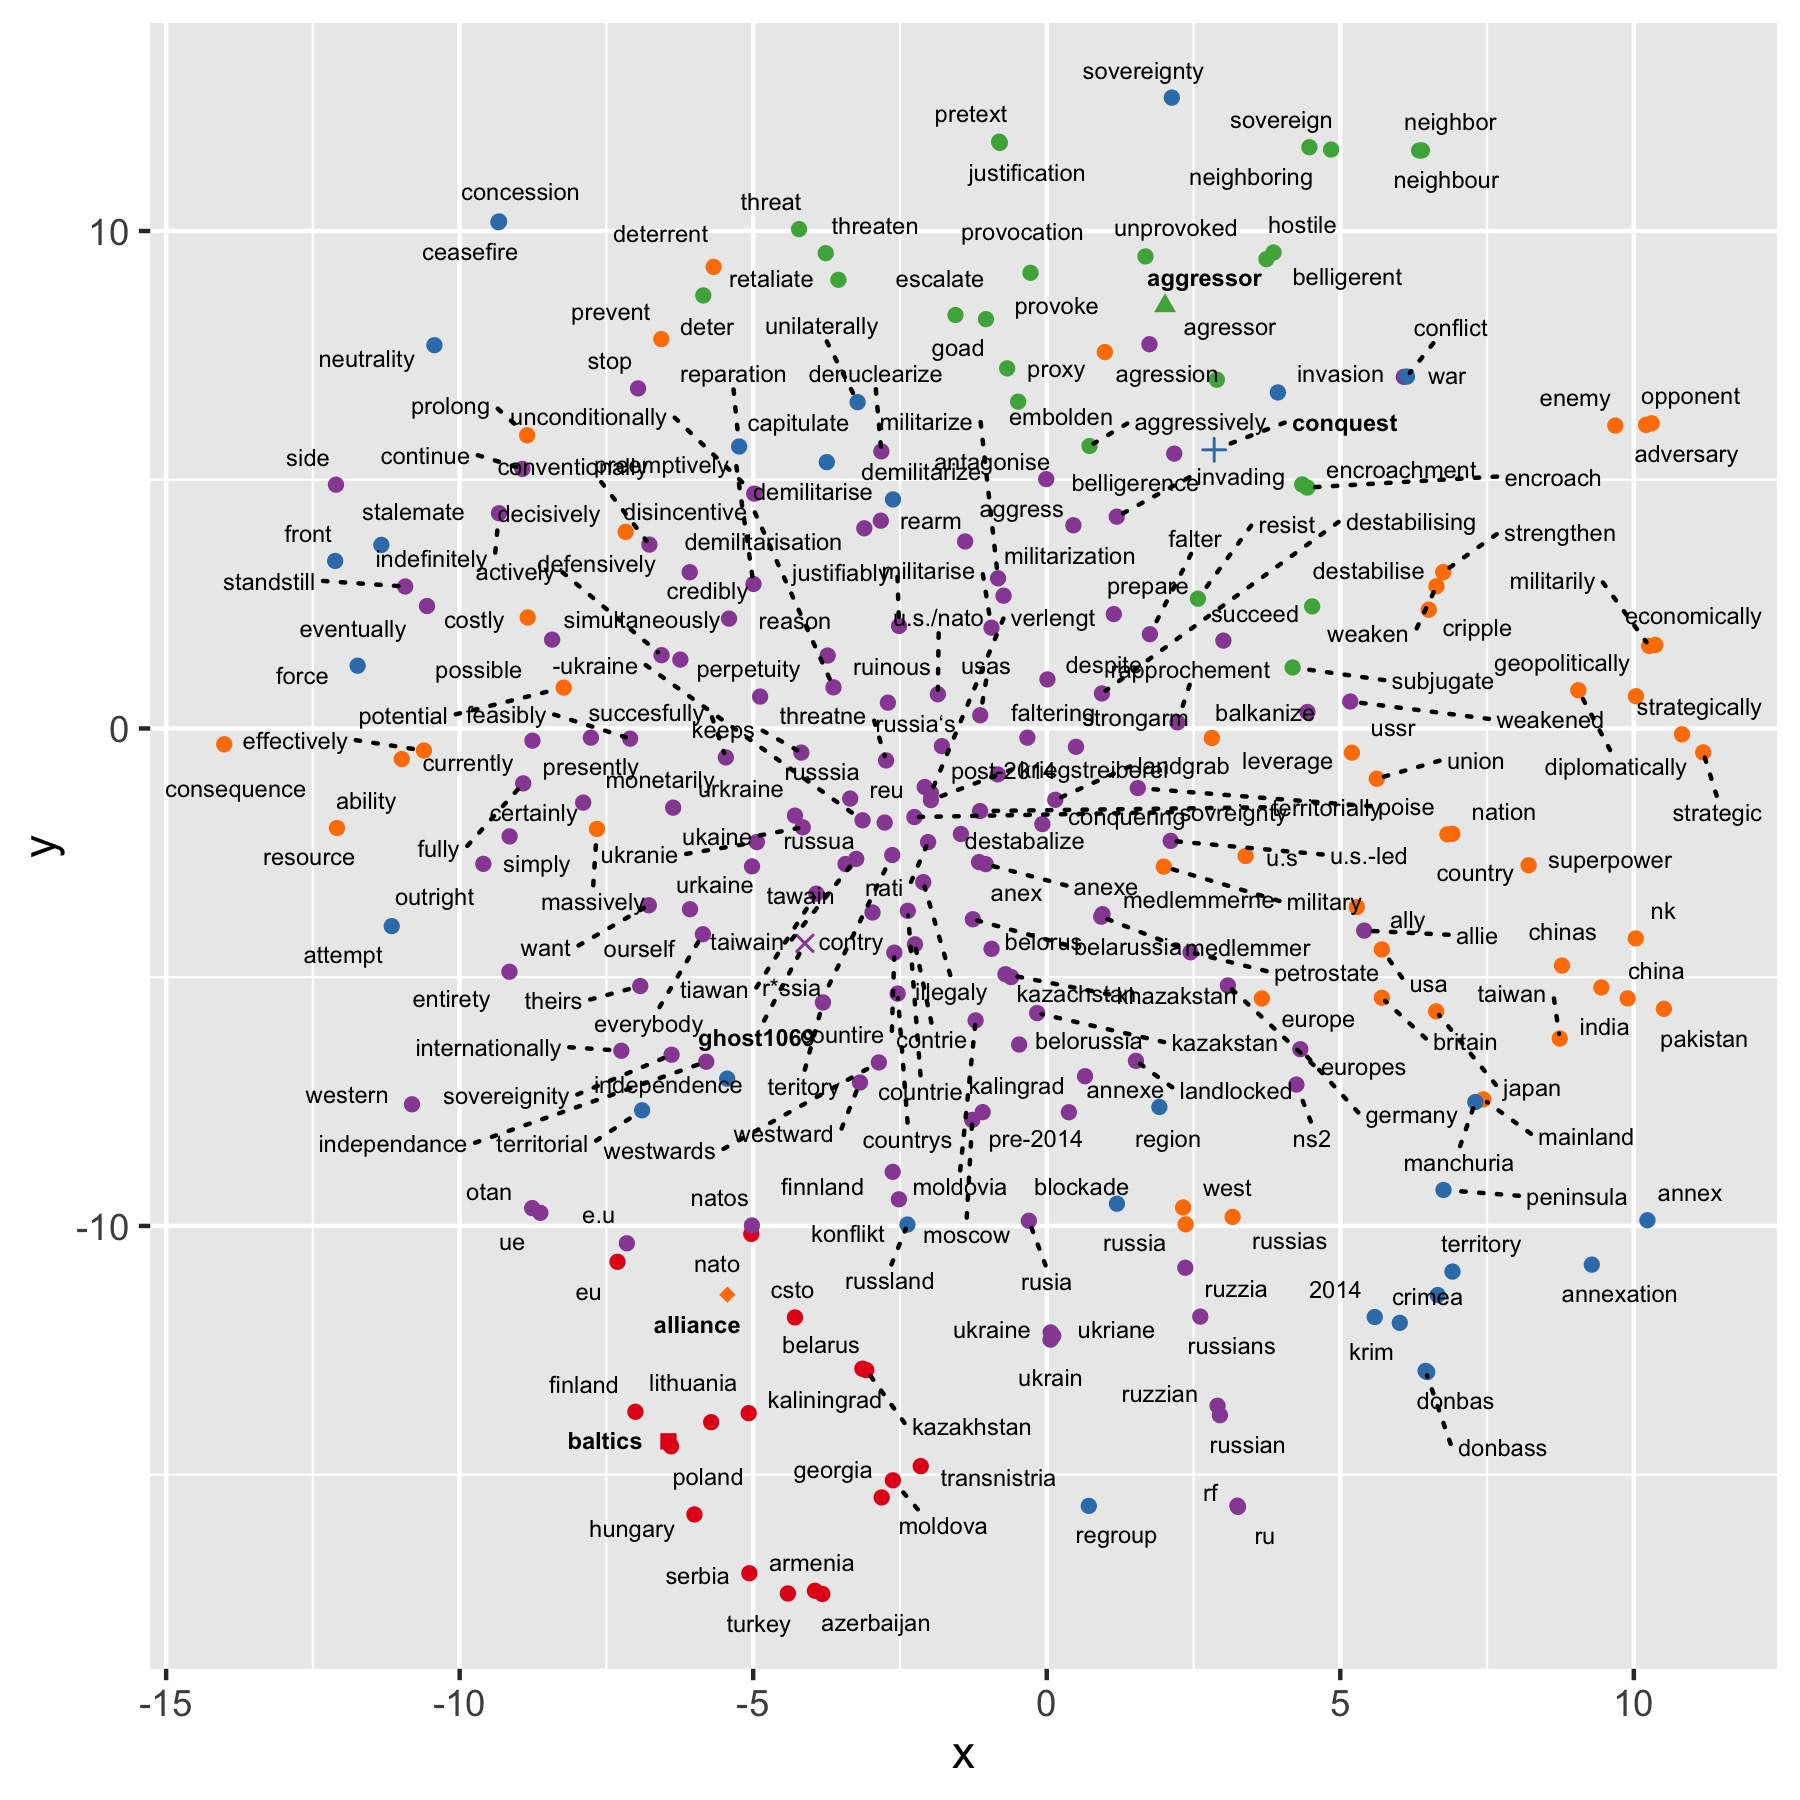
\includegraphics[width=\textwidth]{2022/russia}
\caption{Most-similar to ``russia''}
\label{fig:russia_2022}
\end{figure}

For completeness, Figure \ref{fig:russia_2022} displays the 258 most-similar terms to ``russia'' with 42 excluded.
Russia and Ukraine are often discussed in relation to one another so they present similar terms and clusters.
Towards the bottom of the graph is a \emph{baltics} cluster of nearby states and organizations: \emph{belarus, nato, lithuania, moldova, finland, azerbaijan, kazakhstan, georgia, turkey, poland, transnistria, serbia, kaliningrad, csto, armenia, hungary}.

Nearby, at the bottom-right is the \emph{conquest} cluster: \emph{territory, crimea, demilitarize, russland, donbas(s), 2014, unilaterally, blockade, concession, stalemate, sovereignty, force, reparation, conflict, front, peninsula, neutrality, annex(ation), ceasefire, manchuria, krim, attempt, regroup, independence, capitulate, region, territorial, invasion}.
This is bordered by the \emph{alliance} grouping to the right of the graph which includes countries Russia is competing and cooperating with: \emph{russia(s), west, country, militarily, china, taiwan, europe, nation, ally, usa, mainland, economically, weaken, decisively, india, ussr, prevent, diplomatically, adversary, superpower, pakistan, geopolitically, nk, massively, leverage, effectively, strengthen, proxy, alliance, japan, consequence, deterrent, strategic(ally), chinas, resource, britain, costly, cripple, enemy, u.s, opponent, potential, ability, prolong, military, union}.
Bordering this group, at the top of the graph is the \emph{aggressor} cluster which shares terms with but is more negative than anything in the Ukrainian graph: \emph{neighbor, neighbour, deter, unprovoked, provocation, resist, neighboring, pretext, sovereign, embolden, provoke, hostile, encroachment, retaliate, belligerent, goad, agression, justification, aggressively, escalate, destabilise, threat(en), encroach, subjugate}.

Finally, the \emph{ghost1069} cluster at the center contains a veriety of topics: \emph{ruzzia(n), agress(or), landgrab, pre-2014, petrostate, sovereignity, tiawan, illegaly, demilitarisation, militarize, countire, medlemmerne, taiwain, ruinous, u.s.-led, tawain, destabalize, anex(e), invading, conquering, belligerence, konflikt, destabilising, balkanize, kazakstan, post-2014, medlemmer, rapprochement, khazakstan, justifiably, moldovia, e.u, independance, antagonise, threatne, sovreignty, kriegstreiberei, verlengt, contry, strongarm, militarise, r*ssia, ns2, perpetuity}.
Ghost makes a return, as well as foreign language terms and various spellings.
This cluster tends towards negative notions like aggression but it also is forward-looking with its emphasis on Taiwan (and China's possible moves there) as well as other countries that Russia has shown an interest in like Moldova.
It evokes fear of ongoing conflict.

\section{Discussion}

In this chapter we analyzed conspiracy theories and their increasing use as an effective tool across social media.
Conspiracy theories rely on natural human faults like confirmation bias, tend to use ``the paranoid style'', and are a way for threatened groups to target an ``Other'' as a means of regaining power when faced with limited or confusing information.
These theories are especially adopted by those that have previously been discriminated against, they offer holistic, self-sealing stories that easily adapt to any flaws in existing narratives.
Soviet active measures have long used conspiracy theories as a strategy of increasing social distrust, popular narratives of the last 20 years have included 9/11 truthers, Birtherism, and claims of false flags around major events, including the shooting at Sandy Hook Elementary.
They were used throughout the 2016 US presidential campaign, the Covid-19 pandemic, and the invasion of Ukraine.

We studied discussion around the February 2022 invasion of Ukraine by processing Reddit's submissions and comments from January through June of that year.
There is a sharp spike in activity the day of the invasion (February 24) and then a gradual reduction to lower levels.
This includes discussion in a variety of expected subreddits as well as the citing of a wide-range of mainstream domains, mainly from the United States but also from foreign outlets in the United Kingdom and elsewhere.
Highly-cited Wikipedia articles contain Russian talking points like past foreign regime changes of the United States and claims of neofascism in Ukraine, but also include relevant topics such as the Wagner Group, a private paramilitary organization with direct ties to the Putin regime.

The most-active and connected users tend to favor social media like Twitter and a few specifc subreddits including r/worldnews, but unlike previous chapters do not post large numbers of partisan domains that we preselect into groups.
In the Word2vec analysis, topics of discussion related to Putin, Russia, and Ukraine are especially unfavorable towards Putin and Russia and may show evidence of the influence of Ukrainian propaganda in the so-called ``Ghost of Kyiv''.

What caused the reduction of rus, conservative, and progressive users apparent  throughout Chapter 4?
The rus group in particular, sourced from Chapter 2, is virtually non-existent, especially among the most-connected users, the exact opposite from 2013-2015, where they dominated the top k-shells.
Regarding the conservatives and progressives, many of the more partisan domains simply are not relevant or are not the best sources of information when we shift from a domestic to global context.

It is important to note that the methods used in this chapter are slightly different, because we do not directly match on comments, we only pick up domains that are submitted as stories, as such, it is possible that we are missing users that primarily attempt to influence discussion by commenting.
The analysis of these comments is an obvious choice for future research.
With the processed data, we have two main reasons for this change in behavior: tighter controls by Reddit and user adaptation.

Reddit has publicly stated that after 2016 they began banning Russian and other accounts connected to astroturfing campaigns, YouTube and other sites similarly have banned Russian state media \cite{browne2018}.
This is visible in the data, the user u/vigorous, very prolific in the invasion of Crimea and even found in the 2016 presidential data, as of 2023 has been banned.
It is likely that the most obvious Russian propaganda is identifiable and prevented by site administration.
When it is not, outlets like RT simply do not have the credibility they had as a counterweight to Western interests after the Russian invasion and revelations of incidents like the massacre in Bucha. 

However, just as likely is that Russian propaganda has changed form.
Social media was originally used because of its virality and the immediate metrics it provided, propagandists like other outlets were able to quickly figure out what attracted interest and what did not \cite[p. 28]{woolley2018}.
Prior to the fall of the Soviet Union, scholars observed the apparent ``sophisticated reaction'' of the militaries of the US and USSR adapting to each other through changes in expenditures \cite{williams1988}. 
This happened despite massive bureaucracies and dealt with physical, expensive armaments.
What is changing a social media campaign in comparison?
We should expect rapid iteration, both in the forms of propaganda used (perhaps outlets we have not identified) and in form.
Reddit was important in 2013 and is in 2023, but there are entire networks that did not exist then, like TikTok.
We should not expect the same behavior across a decade, as Reddit is no longer the largest captive audience, it may already be irrelevant, only a secondary arm of today's propaganda.

\chapter{Conclusion}
\epigraph{I remember that the white men were coming to fight us and take away our land, and I thought it was not right. We are humans, too, and God created us all alike, and I was going to do the best I could to defend my nation.  So I started on the warpath when I was 16 years old.}{Fire Thunder}

The preceding chapters analyzed computational propaganda on Reddit from 2013 through 2022.
In the introduction we defined computational propaganda - the use of Big Data, algorithms, bots, and astroturfing campaigns on the Internet and social media at a global, never before seen scale.
Propaganda is ancient but the 20th century saw its rapid development, in the United States through mass media and by figures such as Edward Bernays and in the Soviet Union through the use of active measures - misinformation and disinformation campaigns that target divisions and weaknesses in other countries.
Computational propaganda as practiced by Russia today is only the most recent iteration of this.

We also introduce the concept of framing, or the manner in which a topic is presented.
Disinformation and misinformation are both methods of framing by manipulating the context around a discussion.
Similarly, arguments have dimensionality, or layers, politicians and those involved in arguments can either use rhetoric to ``win'' the discussion over existing issues or they can introduce additional dimensions to reframe the topic and debate in their favor.
This is common on social media where individuals are constantly introducing new viewpoints to existing discussions, not always in good faith.

One final aspect of framing is the notion of selectorate theory.
This political science concept suggests that leaders have multiple audiences that they are responsive to, but their innermost circle, the selectorate,  drives much of their behavior.
It explains Putin's motivations and blindspots in invading Ukraine as well as the failures of Zuckerberg at Facebook and CEOs at other social media companies to notice the presence of computational propaganda on their platforms throughout the 2016 US presidential election.
It is a form of ``echo chamber'', a wider issue which seems to plague much modern media and conversation.

Our analysis of Reddit, and that of social scientists pursuing and communicating similar research must recognize this cultural aspect.
We distinguish between science and scientism and emphasize the importance of empathy and knowing our own biases and limitations.
We build a framework that we follow in each chapter using Python, R, simple heuristics, and applied statistics and algorithms that are modern but above all easy to understand.

First, we choose a timeframe that we download data for, then filter it using keywords and graph and observe temporal trends in the data.
Next, we identify and group users based on which subreddits they post in or which domains they post from using preselected lists of domains.
We are additionally able to study narratives using these extracted domains as well as posted Wikipedia articles which are telling collections of facts and events.
Third, we use various network analysis tools like k-shell composition, betweenness centrality, and in and out-degree to position users and groups of users within the wider network of interacting users in order to discern who most directs and affects discussion.
Finally, using the text from submissions and comments, we train separate high-dimensionality models using Word2vec in order to extract most-similar words for various terms.
We then use t-SNE to reduce these scores to two dimensions, plotting graphs of ``talking points'' clustered by topic using k-means, this gives a visual summary of discussion in under 300 words. 
The summarization in each of these steps is possible because human behavior follows power laws by which a small subset of data, whether users, links, or subreddits tend to represent the majority of activity.
 
Chapter 2 covers the build-up to and annexation of Crimea in February 2014 by Russia.
Putin and oligarchs came to power in the 1990s following the fall of the USSR.
Throughout this time, Russia's tech industry grew in an environment of political and economic openness.
Circa 2005, Russia began using tools like Russia Today to reorient and position itself as a pragmatic competitor to the United States.
By 2012 with the return of Putin to the presidency, this shifted to the restriction of freedoms and the use of computational propaganda at home and abroad as an extension of Soviet/Russian active measures.

In November 2013, Ukraine's Russian-favoring president refused to sign a negotiated agreement with the European Union which would have increased economic and political ties, this led to protests known as Euromaidan starting that month.
February 2014 brought his ouster and he fled the country, in response Russia annexed Crimea and began directly supporting rebels in the Donbas region in eastern Ukraine, a conflict which only nominally was halted with the Minsk agreements in February 2015.

Other researchers found evidence of Russian computational propaganda, trolls, bots, and falsehoods spread by state media across social media at this time.
We study these events on Reddit by filtering data from 2013 through 2015.
Peak activity overlaps, occurring in February 2014, July 2014 when MH17 was shot down over Donbas, and to a lesser extent in November 2013 and February 2015.
Pro-Russian ``superspreaders'' and users are identified based on their posting from a preselected list of Russian state websites and biased or extremist domains. 
These users favor niche, noncredible sources and legalistic arguments from Wikipedia based on whataboutism.
Using various measures of network centrality and connectivity, superspreaders like u/vigorous dominate the most influential positions of the network, and in an analysis of discussions using Word2vec, Russian talking points such as comparing Crimea's annexation to independence movements throughout the world are readily apparent. 

Chapter 3 covers the 2016 presidential election in the United States.
The Mueller Report, released in 2019, details coordinated astroturfing by Russian agents across social media.
This was combined with hacking and contact with Trump campaign officials, summarized as ``systematic and sweeping'' election interference.

We contrast and compare the political cultures of Russia and the United States.
Russia's thousand-year history includes heavy influence by the Eastern Roman (Byzantine) Empire, from which it adopted Orthodox Christianity, the role of the autocrat ruler, and its role as protector of the Slavic peoples.
The United States has a similar expansionist history, but took influence from the political ideas of Western Europe, these were distilled into a designed Constitution and form of government elaborated on at length in the Federalist Papers.
Both countries, but especially the capitalist, democratic US, experienced massive social and political change due to the Industrial Revolution and changing communication technology over the last few hundred years.
Innovations in technology like paper and the printing press had similar effects, but were the process of much more gradual discoveries across many different cultures.
It is this global, instant, mass communication against which the designed political institutions of the United States are not prepared.

Our analysis of Reddit uses filtered relevant data from 2015 through 2017.
User activity corresponds to usual seasonal and campaign cycles, peaking during the primary season, at election time, and during the inauguration, depending on the candidate (Sanders and Clinton supporters are less active after their defeats).
We identify groups of progressive and conservative subreddits by which users are categorized.
The subreddit r/The\_Donald is the most  active of our selected subreddits, but it is an outlier, otherwise progressive subreddits including r/politics and candidate subreddits have much more traffic than conservative.

Progressive and conservatives share common mainstream sources like the New York Times as well as popular social media cites including Twitter.
Each group posts from expected partisan sources, however, conservatives favor niche and conspiratorial sources like InfoWars and Stop the Steal, a pattern which continues in linked Wikipedia articles.

In terms of network analysis, progressives tend to dominate positions of influence, though conservative users are present, likely due to the general progressive tilt of Reddit as a whole.
While r/The\_Donald has fervent supporters, those supporters tend to cluster within that subreddit, not unlike real-life Trump voters.
Textual analysis using Word2vec shows the heavy presence of conspiracy theories like Pizzagate and Russiagate in reference to the Mueller Report, matching Trump's rhetoric of a Deep State coup against him.
Progressive descriptions use more neutral, factual language common to mainstream news articles.
Both groups use negative language to describe each other, but also show similar concerns, especially around popular media.
We note that this preference for alternative sources goes back to the rise of cable television and talk radio apparent by the Gingrich Congress.
Underdogs naturally seek to undermine existing larger players and today every YouTube channel, Twitter account, and Substack has incentive to spread distrust of mainstream media.
 
Finally, Chapter 4 covers the rise of conspiracy theories and their effect on the Russian invasion of Ukraine in 2022.
Conspiracy theories are presumptions of conspiracy, a populist form of power where information or rationality are limited, usually relying on ``the paranoid style''.
They are attractive because they offer unifying explanations of events and a  responsible ``Other''.
Though they feed on human flaws like confirmation bias, they are attractive in an ever-changing world, especially to individuals and groups that have previously faced discrimination.
Conspiracy theories have seen a rise in popularity since the 1990s with claims of false flags around major events.
Trump used them before, during, and after his presidency, and Russian active measures promoted them during the Covid-19 pandemic and the invasion of Ukraine.
 
Our analysis of Reddit uses relevant filtered data from January through June 2022. 
The most activity occurs the first day of the invasion, February 24th, then decreases to lower but still noticeable levels.
We only match on submissions, which may alter the results, but the most popular submitted domains are mainstream sources.
Wikipedia articles include Russian talking points as well as articles critical of Putin and Russia and covering topics such as Yevgeny Prigozhin's Wagner Group.

Social media sites like Twitter are popular among the most-connected users in the network analysis, but notably the majority these users do not belong in the rus, progressive, or conservative groups established in the previous chapters.
The rus group in particular is especially absent, further confirmed in the textual Word2vec analysis which is especially critical of Putin and Russia and shows apparent Ukrainian propaganda such as the ``Ghost of Kyiv''.
We attribute this to more awareness of computational propaganda by Reddit admins, the loss of credibility of Russian sources, as well as the likely shifting of Russian tactics since 2013 to be less obvious and targeting newer social media like TikTok. 

In the introduction we asked two questions.
First, does Reddit show evidence of being captured by ideologically extreme entities like special interest groups or nation-states?
Second, how is this capture affecting objective coverage of events?
Chapter 2 shows obvious capture with pro-Russian users and discourse dominating discussion.
Chapter 3 shows capture within limited groups, for example, conservative users mimic Trump's rhetoric.
In each instance, the discussion is biased towards these entities in an extreme manner, like the presentation of the Mueller investigation as a coup.
Furthermore, our analysis does not examine submissions and comments at an individual level, but a quick perusal of any political subreddit, progressive or conservative, includes heated, othering language.
Some subreddits are less biased and more objective, but the very design of the site encourages sorting into ideological groups.

This leads to open questions.
Russia's system of propaganda is a ``media factory'' of outlets like RT which create content and trolls and bots which distribute it, but which part of the factory are we observing?
Was u/vigorous a paid troll or just a nationalist Russian?
How much of the activity around 2013 or on a subreddit like r/conspiracy is the direct result of agents paid by the Russian state versus second-level users that are absorbing and sharing it?
In comparison to King, Pan, and Roberts (2017) we have no Rosetta Stone, no ground truth data by which to confirm the government connection of identified users \cite{king2017}. 
The organization that has the best data for this kind of analysis is Reddit with Internet (IP) addresses, this allows them to track user behavior and is probably the basis by which many of their bans of Russian users happens.
Sytematic research like this study using that data would be very revealing, but 
can only happen internally.

Domestic organizations present similar issues.
We know of the existence of Correct the Record, which supported Clinton during the 2016 election, but have no easy way of tracking its activity.
The domains shared and discussion generated are from sites and individuals within the United States which means there is less locational data or behavioral data to make this artificial astroturfing stand out from other partisan users.
There is likely the perception that this kind of activity is different than that of paid campaigns which organize people to go door to door, but to what extent?
Candidates, companies, and entities connected to the US government are greatly incentivized to run these campaigns which manipulate public opinion, they are effective precisely because they appear to be organic behavior.
Researchers need better open data from organizations like Reddit.

Researchers also need better tools and research design.
This study is only a demonstration of what is possible using available data, establishing ways of grouping topics and users, and emphasizing the importance of dimensionality.
These tools have rapidly improved just since the start of this dissertation.
Word2vec was created in 2008, but transformer models like BERT promise better mapping of the relationship between words in documents.
This allows us to, for example, disentangle the terms progressive and conservative in the same piece of text, commonly found together but used in comparison to each other.
Part of adopting new tools will not just involve using the latest and greatest, but determining what meets researcher needs while still being easy to use and  understand, only possible over multiple studies.

Finally, text is only the beginning.
Today's social media is already shifting to other mediums including audio and video and to these use of generative models like ChatGPT.
Future studies will need to track similar user networks and metadata as this analysis of Reddit, but they will want to examine the content of the video itself, tracking and detecting recognizable objects and accurately transcribing dialogue.
More challenging will be filtering mass amounts of artificially generated material.
We hope this study provides inspiration towards these future analyses.
For updates, including an extension to this conclusion, please visit \url{http://lebo.io/comprop}.

\begin{thesisbib}
\bibliography{references}
\end{thesisbib}

\begin{biosketch}
Aaron Lebo is from Dallas.
He began programming in 2005 and graduate studies at The University of Texas at Dallas in 2010.
He lives with this dog, Teddy Roosevelt, is interested in history and languages, and works on open source technologies.
\end{biosketch}

\begin{vita}
  \begin{center}
     {\LARGE\bfseries Aaron Lebo} \\[5pt]
     April 17, 2023
   \end{center}

   \bigskip

   {\large\bfseries Contact Information:\par}
   \medskip
   \noindent\vtop{\hsize=.49\hsize
     School of Economic, Political & Policy Sciences\par
     The University of Texas at Dallas\par
     800 W.~Campbell Rd.\par
     Richardson, TX 75080-3021, U.S.A.\par}
   \hfil\vtop{\hsize=.49\hsize
     Voice: (972) 883-2935\par
     Email: \texttt{aaron.lebo@utdallas.edu}\par}\par

   \bigskip

   {\large\bfseries Educational History:\par}
   \medskip
   AS, El Centro College, 2006\par
   BA, Interdisciplinary Studies, The University of Texas at Dallas, 2009\par
   MA, Political Science, The University of Texas at Dallas, 2011\par

   \bigskip

   {\large\bfseries Employment History:\par}
   \medskip
   Research Assistant, The University of Texas at Dallas,
     May 2017~-- March 2021\par
   Programmer, FXdirect, Inc.,
     February 2006~-- December 2017\par
  
\end{vita}

\end{document}

